
% ----------------------------------------------------------------
\vfuzz2pt % Don't report over-full v-boxes if over-edge is small
\hfuzz2pt % Don't report over-full h-boxes if over-edge is small
% THEOREMS -------------------------------------------------------



% MATH -----------------------------------------------------------


% ----------------------------------------------------------------------
%              Latex PhD template for the University of Deusto
% ----------------------------------------------------------------------


%: Style file for Latex
% Most style definitions are in the external file PhDthesisPSnPDF.
% In this template package, it can be found in ./Latex/Classes/
\documentclass[12pt,twoside]{Latex/Classes/PhDthesisPSnPDF}

\usepackage{graphicx}


\newtheorem{thm}{Teorema}[section]
\newtheorem{cor}[thm]{Corolario}
\newtheorem{lem}[thm]{Lema}
\newtheorem{prop}[thm]{Proposición}
\newtheorem{prob}[thm]{Problema}
\newtheorem{defn}[thm]{Definición}


\newtheorem{rem}[thm]{Comentario}

\newtheorem{ejem}[thm]{Ejemplo}

%: Macro file for Latex
% Macros help you summarise frequently repeated Latex commands.
% Here, they are placed in an external file /Latex/Macros/MacroFile1.tex
% An macro that you may use frequently is the figuremacro (see introduction.tex)
\include{Latex/Macros/Macros}


%: ----------------------------------------------------------------------
%:                  TITLE PAGE: name, degree,..
% ----------------------------------------------------------------------
% below is to generate the title page with crest and author name

% if output to PDF then put the following in PDF header
\ifpdf
    \pdfinfo { /Title  (P)
               /Creator (TeX)
               /Producer (pdfTeX)
               /Author (Santiago P\'erez)
               /CreationDate (D:YYYYMMDDhhmmss)  %format D:YYYYMMDDhhmmss
               /ModDate (D:YYYYMMDDhhmm)
               /Subject (xyz)
               /Keywords (keyword1, keyword2, keyword3) }
    \pdfcatalog { /PageMode (/UseOutlines)
                  /OpenAction (fitbh)  }
\fi


% Title of the dissertation
\title{Tesis}


% ----------------------------------------------------------------------
% This section below defines front covert (external and internal)
% Shield logo
\crest{
\includegraphics[width=4cm]{Deusto_Shield}}
% Full logo
%\crest{
\includegraphics[width=6cm]{UDeusto}}
%\university{UNIVERSIDAD NACIONAL AUT\'ONOMA DE M\'EXICO}
\university{\textbf{UNIVERSIDAD NACIONAL AUT\'ONOMA DE M\'EXICO} \ \ \ \ \\
PROGRAMA DE MAESTR\'IA Y DOCTORADO EN CIENCIAS MATEM\'ATICAS Y DE LA ESPECIALIZACI\'ON EN ESTAD\'ISTICA APLICADA}
\collegeordept{ }
\title{Caracterización de Nielsen de grupos discretos de PSL(2,$\mathbb{R}$)}

\degree{TESIS \\ QUE PARA OPTAR POR EL GRADO DE:\\
MAESTRO EN CIENCIAS   \\ } 

\author{  PRESENTA: \\ Santiago Manuel P\'erez P\'erez }

\textadvisor{  }
\advisor{DIRIGIDA POR: \\ Dr. Angel Cano Cordero  \\ Instituto de Matem\'aticas Cuernavaca, UNAM}
\advisortwo{ }
\textsignaturecandidate{}
\textsignatureadvisor{}
\cityofbirth{M\'exico D.F.} 
%\degreedate{Marzo de \ \the\year}
\degreedate{Marzo de \the\year}


% ----------------------------------------------------------------------

% turn of those nasty overfull and underfull hboxes
\hbadness=10000
\hfuzz=50pt


%: --------------------------------------------------------------
%:                  FRONT MATTER: dedications, abstract,..
% --------------------------------------------------------------


\begin{document}



\selectlanguage{spanish}

% sets line spacing
%\renewcommand\baselinestretch{3}
 %\baselineskip=18pt plus1pt

% Watermark
%\watermark{DRAFT	DRAFT	DRAFT	DRAFT	DRAFT	DRAFT	DRAFT	DRAFT	DRAFT}


%: ----------------------- generate cover page ------------------------

\maketitle  % command to print the title page with above variables

% Title back
%% Thesis Titleback ---------------------------------------------------

\thispagestyle{empty}

\hfill

\vfill

\medskip


\noindent
\textit{
Dissertation Title
}




Author: Name

Advisor: Name

Advisor: Name



\vfill

\vfill

\noindent
The following web-page address contains up to date information about this dissertation and related topics: \\
\url{http://paginaspersonales.deusto.es/Name/}


\noindent
Text printed in Bilbao

% TODO final date
\noindent
First edition, 
% Moth and year
\monthname \ \the\year

\vspace{1cm}
\hrule
\bigskip

% \cleardoublepage command ends the current page and causes all figures and tables that have so far appeared in the input to be printed. In a two-sided printing style, it also makes the next page a right-hand (odd-numbered) page, producing a blank page if necessary. 
\cleardoublepage

%%: ----------------------- cover page back side ------------------------
%% Your research institution may require reviewer names, etc.
%% This cover back side is required by Dresden Med Fac; uncomment if needed.
%
%\newpage
%\vspace{10mm}
%1. Reviewer: Name
%
%\vspace{10mm}
%2. Reviewer: 
%
%\vspace{20mm}
%Day of the defense:
%
%\vspace{20mm}
%\hspace{70mm}Signature from head of PhD committee:
%
%
%\cleardoublepage

% ----------------------------------------------------------------------





%: ----------------------- abstract ------------------------

% Your institution may have specific regulations if you need an abstract and where it is to be placed in the document. The default here is just after title.


% The original template provides and abstractseparate environment, if your institution requires them to be separate. I think it's easier to print the abstract from the complete thesis by restricting printing to the relevant page.
% \begin{abstractseparate}
%   
% Thesis Abstract -----------------------------------------------------


%\begin{abstractslong}    %uncommenting this line, gives a different abstract heading


%\begin{abstracts}        %this creates the heading for the abstract page
%\selectlanguage{british}
% Put your abstract or summary here.

%Cuando tenemos una ecuaci\'on diferencial de grado $n$, sabemos gracias a un teorema de Cauchy que posee $n$ soluciones linealmente independientes en un punto $b \in \mathbb{C}$, si tomamos una de estas soluciones y la continuamos anal\'iticamente por un lazo anclado en $b$ obtenemos una soluci\'on que depende de las $n$ soluciones linealmente independientes dadas, gracias a este hecho, podemos de igual manera asociar un grupo a la ecuaci\'on diferencial dada, este grupo visto en $GL(2,\mathbb{C})$ contiene las matrices, llamadas matrices de conexi\'on , que relacionan a la soluci\'on original y a la continuaci\'on anal\'itica de la soluci\'on. Dado un conjunto de soluciones alrededor de un punto  $b \in \mathbb{C} $ y a la continuaci\'on anal\'itica a travez de los lazos en el grupo fundamental $\Pi_{1} (b,\mathbb{C})$ el grupo de matrices de las que se habl\'o anteriormente es llamado el grupo de monodrom\'ia.

%\begin{figure}[h]
 % \centering
  % Requires \usepackage{graphicx}
  %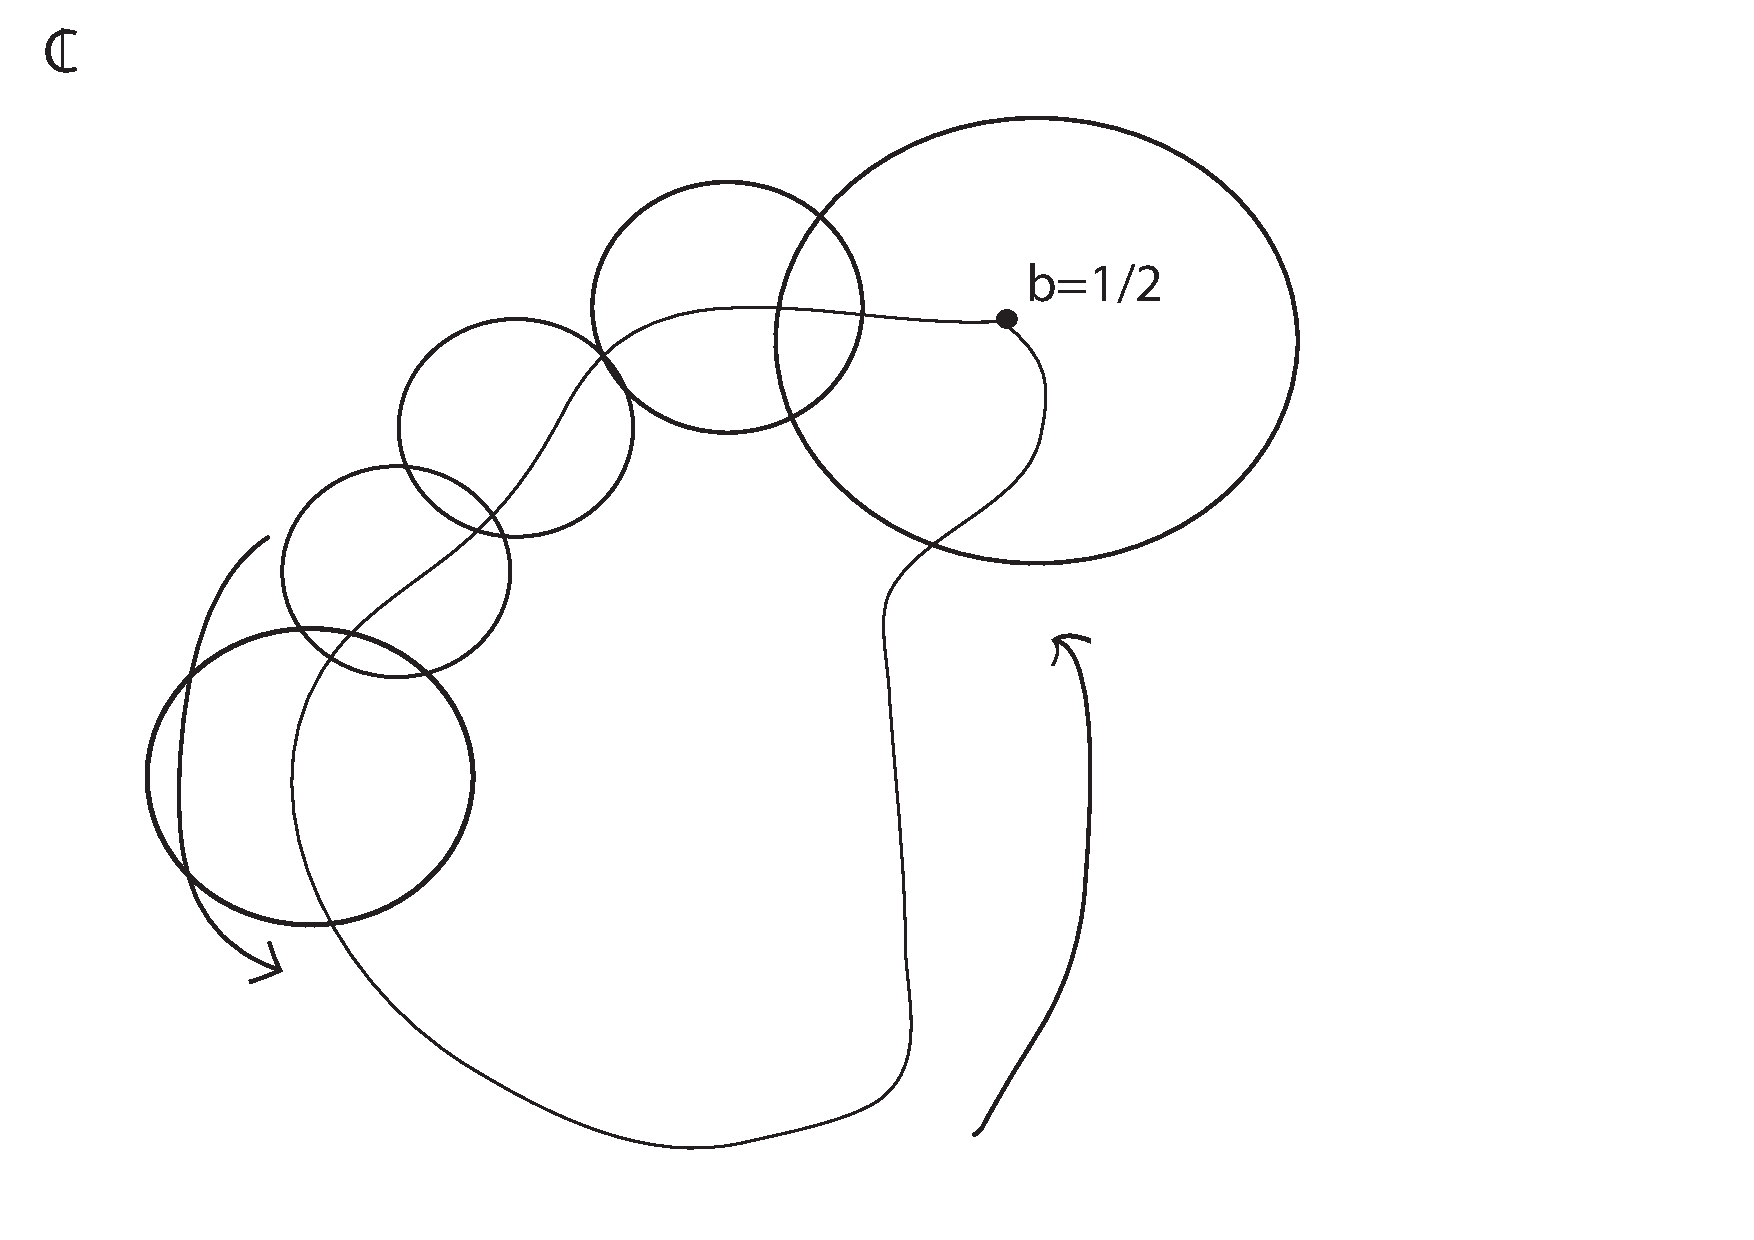
\includegraphics[width=10cm]{abstract-dibujo1}\\
  %\caption{Continuaci\'on anal\'itica}
%\end{figure}




%El grupo de monodrom\'ia nos da informaci\'on importante  de la ecuaci\'on diferencial. En general hallar la monodrom\'ia relativa a una ecuaci\'on diferencial no es una tarea sencilla . Dado este hecho, nos proponemos  hallar y dar de manera expl\'icita la monodrom\'ia y el grupo de monodrom\'ia de la ecuaci\'on diferencial hipergeom\'etrica

 %$$x(1-x)\frac{d^{2}u}{dx^{2}} +  \lbrace c- (a+b+1 )x \rbrace \frac{du}{dx} - abu=0 $$

 %Por medio de una combinaci\'on de t\'ecnicas recopiladas de numerosos textos (de manera particular en \cite{gausspainleve}), adem\'as de dar un conjunto de soluciones para esta ecuaci\'on en el punto $b=\frac{1}{2}$.\\



%El grupo de monodrom\'ia de la ecuaci\'on hipergeom\'etrica tiene una estructura de grupo de Schottky cuando tomamos los exponentes puramente imaginarios, los exponentes dados por

%$$1-c = i\theta_{0}, c-a-b = i\theta_{1},a-b=i\theta_{2} $$

%Con $\theta_{i} > 0$.

%Podemos describir la monodrom\'ia de la ecuaci\'on diferencial hipergeom\'etrica por medio de reflexiones respecto a c\'irculos $C(c,r)$ (donde $c$ es real)

%$$\psi (c,r):s \mapsto \frac{r^{2}}{\bar{s} -c} +c$$

%Y con estas reflexiones asociarle un grupo de Schottky, todo esto siguiendo los pasos de Takashi Ichikawa y Masaaki Yoshida  en una publicaci\'on titulada "ON SCHOTTKY GROUPS ARISING FROM THE HYPERGEOMETRIC EQUATION WITH IMAGINARY EXPONENTS" (\cite{Masaaki}).

%El grupo de Schottky $\Lambda_{\theta}$ asociado a la ecuaci\'on hipergeom\'etrica con exponentes imaginarios nos sirve de ejemplo en un teorema sobre grupos de isometrias del plano hiperb\'olico que act\'uan de manera discontinua en el cual se destaca su prueba casi completamente geom\'etrica propuesta en un art\'iculo de W. Fenchel y J. Nielsen llamado "ON DISCONTINOUS GROUPS OF ISOMETRIC TRANSFORMATIONS OF THE NON-EUCLIDIAN PLANE" publicado en el año de 1948 (\cite{Nielsen}), aunque dado que tenemos 3 parametros $\theta_{1},\theta_{2},\theta_{3}$, en realidad hemos dado muchos ejemplos que cumplen de igual manera este prop\'osito.


%Para obtener este resultado usamos la noci\'on de grupo \textit{elemental} que definimos enseguida.

%\begin{defn}
%\label{def:elemental}
%Un grupo es elemental si su conjunto l\'imite esta formado a lo m\'as por dos puntos
%\end{defn}

%La caracteristica que realmente es de \'interes para nosotros es que un grupo sea NO-elemental, dicho grupo es por lo tanto un grupo cuyo conjunto l\'imite esta formado por  mas de dos puntos.
%En \cite{Nielsen} tenemos la siguiente definici\'on;

%\begin{defn}
%\label{def:discontinuo2}
%Un grupo $G$ se dice discontinuo en un punto $x \in \mathbb{D}$ si $x$ no es un punto de acumulaci\'on de la clase $Gx$
%\end{defn}

%Nuestro objetivo es encontrar ejemplos de grupos que actuen de manera discontinua en $\mathbb{D}$ y verificar en ellos las condiciones del teorema de Nielsen. Los grupos de Schottky que hallamos son discretos y adem\'as son No-elementales estas caracteristicas implican que se cumple en $\mathbb{D}$ la siguiente definici\'on;



%\begin{defn}
%\label{def:discontinuo1}
%Sea $X$ un espacio topologico arbitrario y $G$ un grupo de homeomorfismos de $X$ en $X$. Se dice que $G$ act\'ua discontinuamente en $X$ si y solo si para cada subconjunto compacto $K$ de $X$ se tiene,

%$$g(K) \cap K = \emptyset $$

%Excepto para un n\'umero finito de $g$'s en $G$
%\end{defn}

%Los ejemplos que encontramos satisfacen lo que deseamos gracias a un teorema que podemos encontrar en  \cite{Beardon}, pero tambi\'en gracias a que \ref{def:discontinuo1} implica \ref{def:discontinuo2}, de esta manera sabemos de antemano que nuestros grupos act\'uan de manera discontinua pero tambi\'en nos interesa indagar las condiciones que el teorema de Nielsen requiere y deducir algunas propiedades ya que la demostraci\'on de este teorema en \cite{Nielsen} aclara el comportamiento geom\'etrico de los grupos de transformaciones hiperb\'olicas.




%\end{abstracts}

\begin{resumen}        %this creates the heading for the abstract page
\selectlanguage{spanish}

\renewcommand\baselinestretch{3}

Cuando tenemos una ecuaci\'on diferencial de grado $n$, sabemos gracias a un teorema de Cauchy que posee $n$ soluciones linealmente independientes en un punto $b \in \mathbb{C}$, si tomamos una de estas soluciones y la continuamos anal\'iticamente por un lazo anclado en $b$ obtenemos una soluci\'on que depende de las $n$ soluciones linealmente independientes dadas, gracias a este hecho, podemos de igual manera asociar un grupo a la ecuaci\'on diferencial dada, este grupo visto en $GL(2,\mathbb{C})$ contiene las matrices, llamadas matrices de conexi\'on , que relacionan a la soluci\'on original y a la continuaci\'on anal\'itica de la soluci\'on. Dado un conjunto de soluciones alrededor de un punto  $b \in \mathbb{C} $ y a la continuaci\'on anal\'itica a travez de los lazos en el grupo fundamental $\Pi_{1} (b,\mathbb{C})$ el grupo de matrices de las que se habl\'o anteriormente es llamado el grupo de monodrom\'ia.

\begin{figure}[h]
  \centering
  % Requires \usepackage{graphicx}
  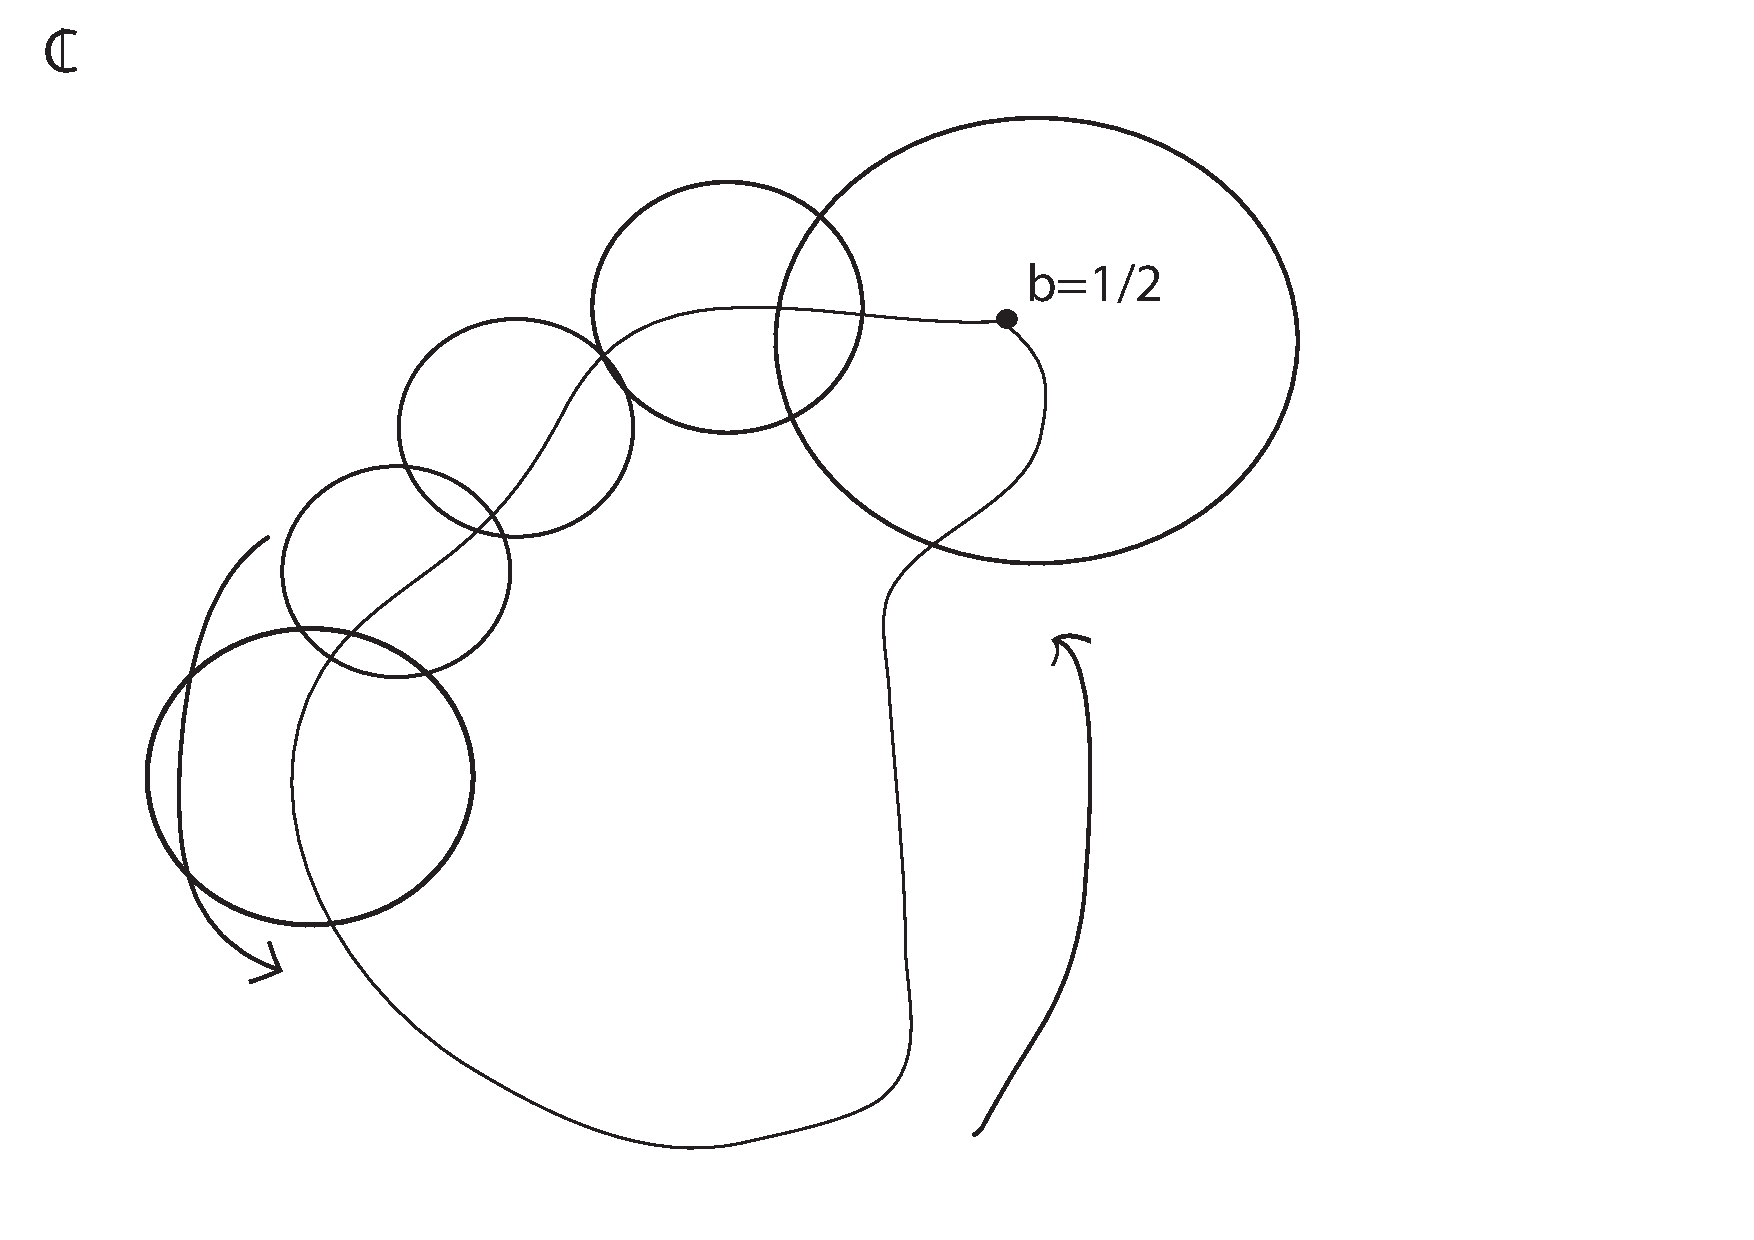
\includegraphics[width=10cm]{abstract-dibujo1.pdf}\\
  \caption{Continuaci\'on anal\'itica}
\end{figure}




El grupo de monodrom\'ia nos da informaci\'on importante  de la ecuaci\'on diferencial. En general hallar la monodrom\'ia relativa a una ecuaci\'on diferencial no es una tarea sencilla . %Dado este hecho,   
Nos proponemos  hallar y dar de manera expl\'icita %la monodrom\'ia y
el grupo de monodrom\'ia de la ecuaci\'on diferencial hipergeom\'etrica.

 $$x(1-x)\frac{d^{2}u}{dx^{2}} +  \lbrace c- (a+b+1 )x \rbrace \frac{du}{dx} - abu=0 $$

 Por medio de una combinaci\'on de t\'ecnicas recopiladas de numerosos textos (de manera particular en \cite{gausspainleve}), adem\'as de dar un conjunto de soluciones para esta ecuaci\'on en el punto $b=\frac{1}{2}$.\\



El grupo de monodrom\'ia de la ecuaci\'on hipergeom\'etrica tiene una estructura de grupo de Schottky cuando tomamos los exponentes puramente imaginarios, los exponentes dados por

$$1-c = i\theta_{0}, c-a-b = i\theta_{1},a-b=i\theta_{2} $$

Con $\theta_{i} > 0$.

Podemos describir la monodrom\'ia de la ecuaci\'on diferencial hipergeom\'etrica por medio de reflexiones respecto a c\'irculos $C(c,r)$ (donde $c$ es real)

$$\psi (c,r):s \mapsto \frac{r^{2}}{\bar{s} -c} +c$$

Y con estas reflexiones asociarle un grupo de Schottky, todo esto siguiendo los pasos de Takashi Ichikawa y Masaaki Yoshida  en una publicaci\'on titulada "ON SCHOTTKY GROUPS ARISING FROM THE HYPERGEOMETRIC EQUATION WITH IMAGINARY EXPONENTS" (\cite{Masaaki}).

El grupo de Schottky $\Lambda_{\theta}$ asociado a la ecuaci\'on hipergeom\'etrica con exponentes imaginarios nos sirve de ejemplo en un teorema sobre grupos de isometrias del plano hiperb\'olico que act\'uan de manera discontinua en el cual se destaca su prueba casi completamente geom\'etrica propuesta en un art\'iculo de W. Fenchel y J. Nielsen llamado "ON DISCONTINOUS GROUPS OF ISOMETRIC TRANSFORMATIONS OF THE NON-EUCLIDIAN PLANE" publicado en el año de 1948 (\cite{Nielsen}), aunque dado que tenemos 3 parametros $\theta_{1},\theta_{2},\theta_{3}$, en realidad hemos dado muchos ejemplos que cumplen de igual manera este prop\'osito.


Para obtener este resultado usamos la noci\'on de grupo \textit{elemental} que definimos enseguida.

\begin{defn}
\label{def:elemental}
Un grupo es elemental si su conjunto l\'imite esta formado a lo m\'as por dos puntos
\end{defn}

La caracteristica que realmente es de \'interes para nosotros es que un grupo sea NO-elemental, dicho grupo es por lo tanto un grupo cuyo conjunto l\'imite esta formado por  mas de dos puntos.
En \cite{Nielsen} tenemos la siguiente definici\'on;

\begin{defn}
\label{def:discontinuo2}
Un grupo $G$ se dice discontinuo en un punto $x \in \mathbb{D}$ si $x$ no es un punto de acumulaci\'on de la clase $Gx$
\end{defn}

Nuestro objetivo es encontrar ejemplos de grupos que actuen de manera discontinua en $\mathbb{D}$ y verificar en ellos las condiciones del teorema de Nielsen. Los grupos de Schottky que hallamos son discretos y adem\'as son No-elementales estas caracteristicas implican que se cumple en $\mathbb{D}$ la siguiente definici\'on;



\begin{defn}
\label{def:discontinuo1}
Sea $X$ un espacio topologico arbitrario y $G$ un grupo de homeomorfismos de $X$ en $X$. Se dice que $G$ act\'ua discontinuamente en $X$ si y solo si para cada subconjunto compacto $K$ de $X$ se tiene,

$$g(K) \cap K = \emptyset $$

Excepto para un n\'umero finito de $g$'s en $G$
\end{defn}

Los ejemplos que encontramos satisfacen lo que deseamos gracias a un teorema que podemos encontrar en  \cite{Beardon}, pero tambi\'en gracias a que \ref{def:discontinuo1} implica \ref{def:discontinuo2}, de esta manera sabemos de antemano que nuestros grupos act\'uan de manera discontinua pero tambi\'en nos interesa indagar las condiciones que el teorema de Nielsen requiere y deducir algunas propiedades ya que la demostraci\'on de este teorema en \cite{Nielsen} aclara el comportamiento geom\'etrico de los grupos de transformaciones hiperb\'olicas.

El cap\'itulo 1 y 2 nos dan las bases para el desarrollo de este trabajo. El cap\'itulo 1 esta basado en las definiciones necesarias como continuación anal\'itica , grupos Klenianos y de Schottky as\'i como una  introducción de la ecuación diferencial hipergeom\'etrica.

En el cap\'itulo 2 hablamos de la monodrom\'ia en general, el esquema de Riemann, calculamos la monodrom\'ia de la ecuaci\'on hipergemo\'etrica y hallamos el grupo de monodrom\'ia con las soluciones dadas por la serie hipergeom\'etrica.


En el cap\'itulo 3 construimos el grupo de schottky asociado al grupo de monodrom\'ia a trav\'es de los dominios fundamentales dados en (\cite{Masaaki})dicho grupo generado por reflexiones nos servira como ejemplo para el teorema principal.

En el cap\'itulo 4 probamos el teorema de Nielsen en 2 partes, la primera parte se prueba de manera sencilla bajo el supuesto de que en el grupo $G<PSL(2,\mathbb{R})$ existen elementos el\'ipticos, la segunda parte supone que no existen elementos el\'ipticos en el grupo y se utilizan 5 lemas para probar el teorema, estos lemas destacan mayormente por sus demostraciones puramente geom\'etricas asi como la demostraci\'on del teorema, al final probamos que el grupo de Schottky encontrado aplica en el teorema de Nielsen.      



\end{resumen}


%\begin{laburpena}        %this creates the heading for the abstract page
%\selectlanguage{basque}
% Jarri zure laburpena hemen.
%\end{laburpena}

%\end{abstractlongs}


% ----------------------------------------------------------------------

% \end{abstractseparate}


%: ----------------------- tie in front matter ------------------------

% The frontmatter text starts here
\frontmatter

%% Thesis Dedictation ---------------------------------------------------

\begin{dedication} %this creates the heading for the dedication page

\textit{Zuk nahi duzuna.}

\end{dedication}

% ----------------------------------------------------------------------


% Thesis Abstract -----------------------------------------------------


%\begin{abstractslong}    %uncommenting this line, gives a different abstract heading


%\begin{abstracts}        %this creates the heading for the abstract page
%\selectlanguage{british}
% Put your abstract or summary here.

%Cuando tenemos una ecuaci\'on diferencial de grado $n$, sabemos gracias a un teorema de Cauchy que posee $n$ soluciones linealmente independientes en un punto $b \in \mathbb{C}$, si tomamos una de estas soluciones y la continuamos anal\'iticamente por un lazo anclado en $b$ obtenemos una soluci\'on que depende de las $n$ soluciones linealmente independientes dadas, gracias a este hecho, podemos de igual manera asociar un grupo a la ecuaci\'on diferencial dada, este grupo visto en $GL(2,\mathbb{C})$ contiene las matrices, llamadas matrices de conexi\'on , que relacionan a la soluci\'on original y a la continuaci\'on anal\'itica de la soluci\'on. Dado un conjunto de soluciones alrededor de un punto  $b \in \mathbb{C} $ y a la continuaci\'on anal\'itica a travez de los lazos en el grupo fundamental $\Pi_{1} (b,\mathbb{C})$ el grupo de matrices de las que se habl\'o anteriormente es llamado el grupo de monodrom\'ia.

%\begin{figure}[h]
 % \centering
  % Requires \usepackage{graphicx}
  %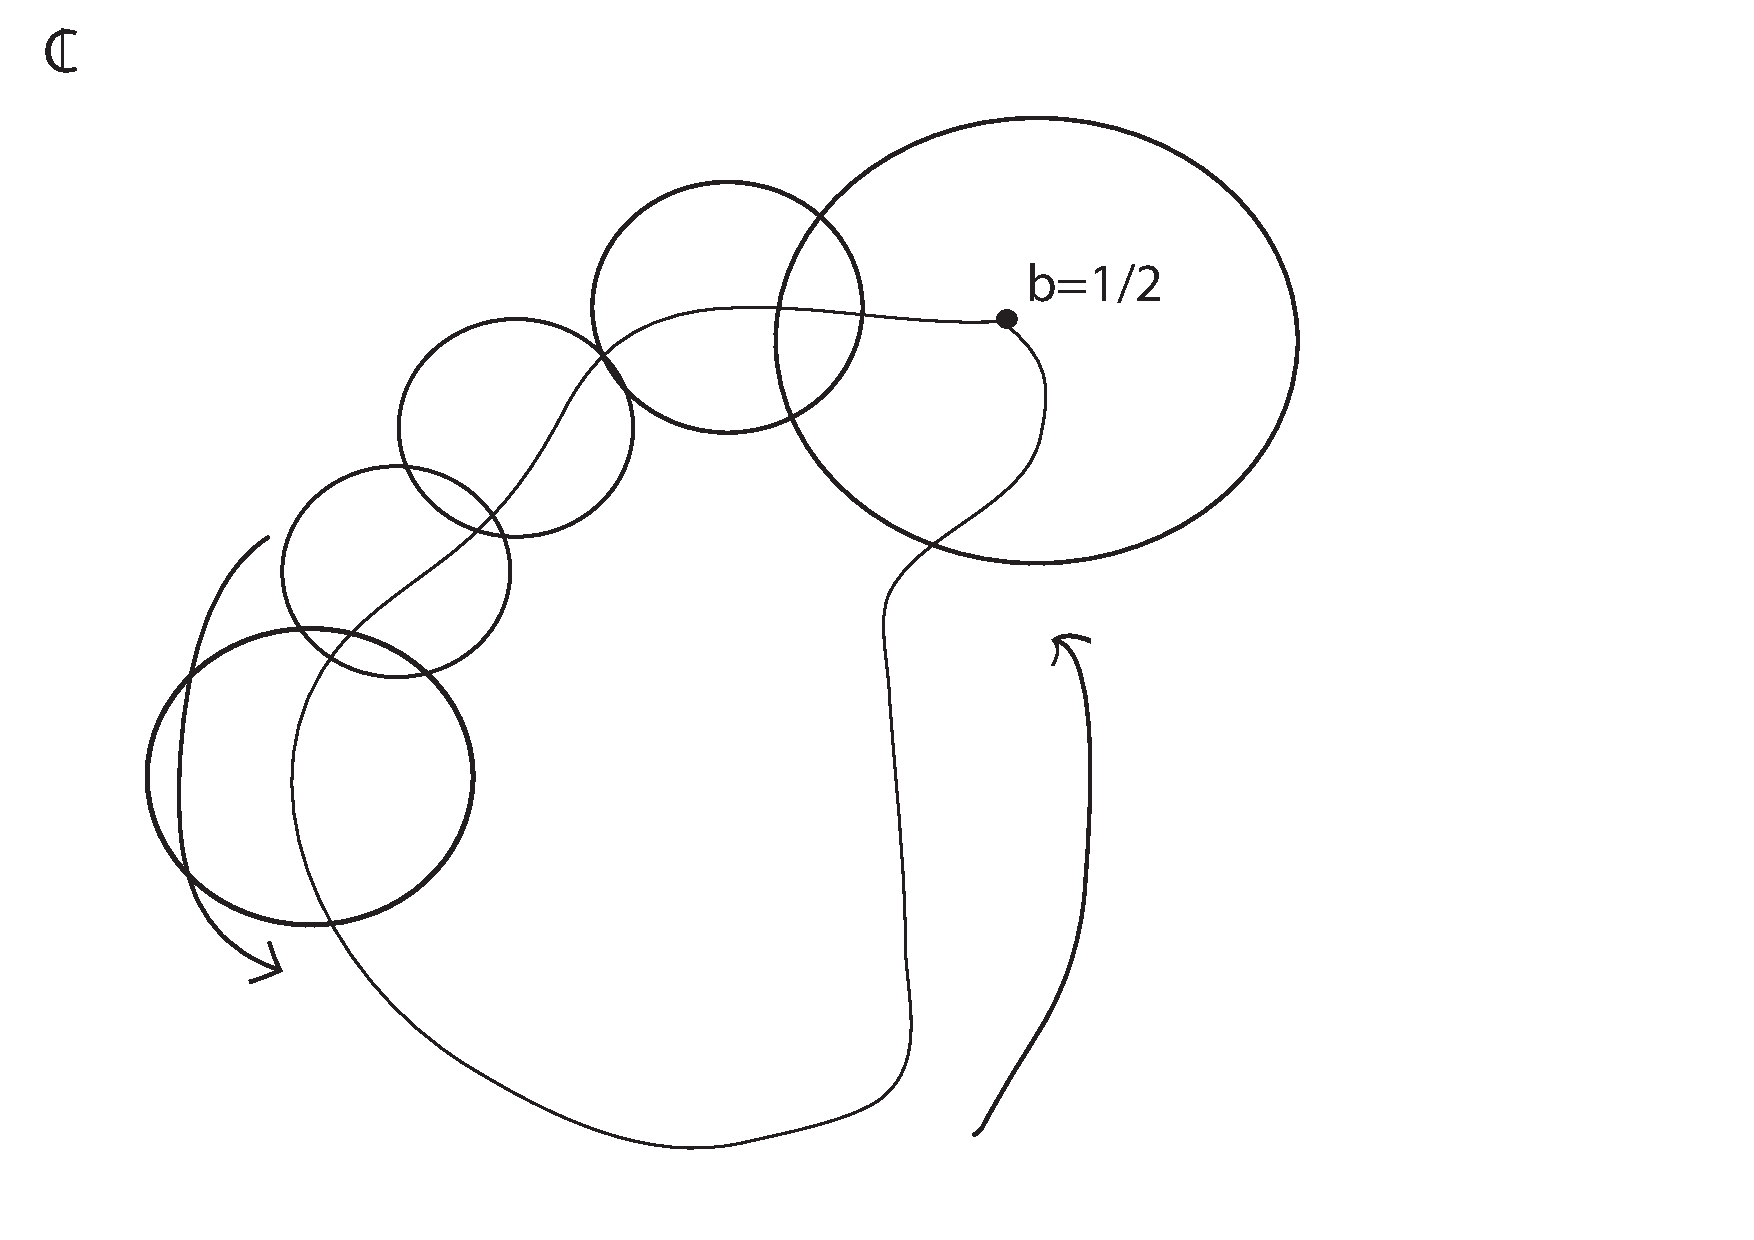
\includegraphics[width=10cm]{abstract-dibujo1}\\
  %\caption{Continuaci\'on anal\'itica}
%\end{figure}




%El grupo de monodrom\'ia nos da informaci\'on importante  de la ecuaci\'on diferencial. En general hallar la monodrom\'ia relativa a una ecuaci\'on diferencial no es una tarea sencilla . Dado este hecho, nos proponemos  hallar y dar de manera expl\'icita la monodrom\'ia y el grupo de monodrom\'ia de la ecuaci\'on diferencial hipergeom\'etrica

 %$$x(1-x)\frac{d^{2}u}{dx^{2}} +  \lbrace c- (a+b+1 )x \rbrace \frac{du}{dx} - abu=0 $$

 %Por medio de una combinaci\'on de t\'ecnicas recopiladas de numerosos textos (de manera particular en \cite{gausspainleve}), adem\'as de dar un conjunto de soluciones para esta ecuaci\'on en el punto $b=\frac{1}{2}$.\\



%El grupo de monodrom\'ia de la ecuaci\'on hipergeom\'etrica tiene una estructura de grupo de Schottky cuando tomamos los exponentes puramente imaginarios, los exponentes dados por

%$$1-c = i\theta_{0}, c-a-b = i\theta_{1},a-b=i\theta_{2} $$

%Con $\theta_{i} > 0$.

%Podemos describir la monodrom\'ia de la ecuaci\'on diferencial hipergeom\'etrica por medio de reflexiones respecto a c\'irculos $C(c,r)$ (donde $c$ es real)

%$$\psi (c,r):s \mapsto \frac{r^{2}}{\bar{s} -c} +c$$

%Y con estas reflexiones asociarle un grupo de Schottky, todo esto siguiendo los pasos de Takashi Ichikawa y Masaaki Yoshida  en una publicaci\'on titulada "ON SCHOTTKY GROUPS ARISING FROM THE HYPERGEOMETRIC EQUATION WITH IMAGINARY EXPONENTS" (\cite{Masaaki}).

%El grupo de Schottky $\Lambda_{\theta}$ asociado a la ecuaci\'on hipergeom\'etrica con exponentes imaginarios nos sirve de ejemplo en un teorema sobre grupos de isometrias del plano hiperb\'olico que act\'uan de manera discontinua en el cual se destaca su prueba casi completamente geom\'etrica propuesta en un art\'iculo de W. Fenchel y J. Nielsen llamado "ON DISCONTINOUS GROUPS OF ISOMETRIC TRANSFORMATIONS OF THE NON-EUCLIDIAN PLANE" publicado en el año de 1948 (\cite{Nielsen}), aunque dado que tenemos 3 parametros $\theta_{1},\theta_{2},\theta_{3}$, en realidad hemos dado muchos ejemplos que cumplen de igual manera este prop\'osito.


%Para obtener este resultado usamos la noci\'on de grupo \textit{elemental} que definimos enseguida.

%\begin{defn}
%\label{def:elemental}
%Un grupo es elemental si su conjunto l\'imite esta formado a lo m\'as por dos puntos
%\end{defn}

%La caracteristica que realmente es de \'interes para nosotros es que un grupo sea NO-elemental, dicho grupo es por lo tanto un grupo cuyo conjunto l\'imite esta formado por  mas de dos puntos.
%En \cite{Nielsen} tenemos la siguiente definici\'on;

%\begin{defn}
%\label{def:discontinuo2}
%Un grupo $G$ se dice discontinuo en un punto $x \in \mathbb{D}$ si $x$ no es un punto de acumulaci\'on de la clase $Gx$
%\end{defn}

%Nuestro objetivo es encontrar ejemplos de grupos que actuen de manera discontinua en $\mathbb{D}$ y verificar en ellos las condiciones del teorema de Nielsen. Los grupos de Schottky que hallamos son discretos y adem\'as son No-elementales estas caracteristicas implican que se cumple en $\mathbb{D}$ la siguiente definici\'on;



%\begin{defn}
%\label{def:discontinuo1}
%Sea $X$ un espacio topologico arbitrario y $G$ un grupo de homeomorfismos de $X$ en $X$. Se dice que $G$ act\'ua discontinuamente en $X$ si y solo si para cada subconjunto compacto $K$ de $X$ se tiene,

%$$g(K) \cap K = \emptyset $$

%Excepto para un n\'umero finito de $g$'s en $G$
%\end{defn}

%Los ejemplos que encontramos satisfacen lo que deseamos gracias a un teorema que podemos encontrar en  \cite{Beardon}, pero tambi\'en gracias a que \ref{def:discontinuo1} implica \ref{def:discontinuo2}, de esta manera sabemos de antemano que nuestros grupos act\'uan de manera discontinua pero tambi\'en nos interesa indagar las condiciones que el teorema de Nielsen requiere y deducir algunas propiedades ya que la demostraci\'on de este teorema en \cite{Nielsen} aclara el comportamiento geom\'etrico de los grupos de transformaciones hiperb\'olicas.




%\end{abstracts}

\begin{resumen}        %this creates the heading for the abstract page
\selectlanguage{spanish}

\renewcommand\baselinestretch{3}

Cuando tenemos una ecuaci\'on diferencial de grado $n$, sabemos gracias a un teorema de Cauchy que posee $n$ soluciones linealmente independientes en un punto $b \in \mathbb{C}$, si tomamos una de estas soluciones y la continuamos anal\'iticamente por un lazo anclado en $b$ obtenemos una soluci\'on que depende de las $n$ soluciones linealmente independientes dadas, gracias a este hecho, podemos de igual manera asociar un grupo a la ecuaci\'on diferencial dada, este grupo visto en $GL(2,\mathbb{C})$ contiene las matrices, llamadas matrices de conexi\'on , que relacionan a la soluci\'on original y a la continuaci\'on anal\'itica de la soluci\'on. Dado un conjunto de soluciones alrededor de un punto  $b \in \mathbb{C} $ y a la continuaci\'on anal\'itica a travez de los lazos en el grupo fundamental $\Pi_{1} (b,\mathbb{C})$ el grupo de matrices de las que se habl\'o anteriormente es llamado el grupo de monodrom\'ia.

\begin{figure}[h]
  \centering
  % Requires \usepackage{graphicx}
  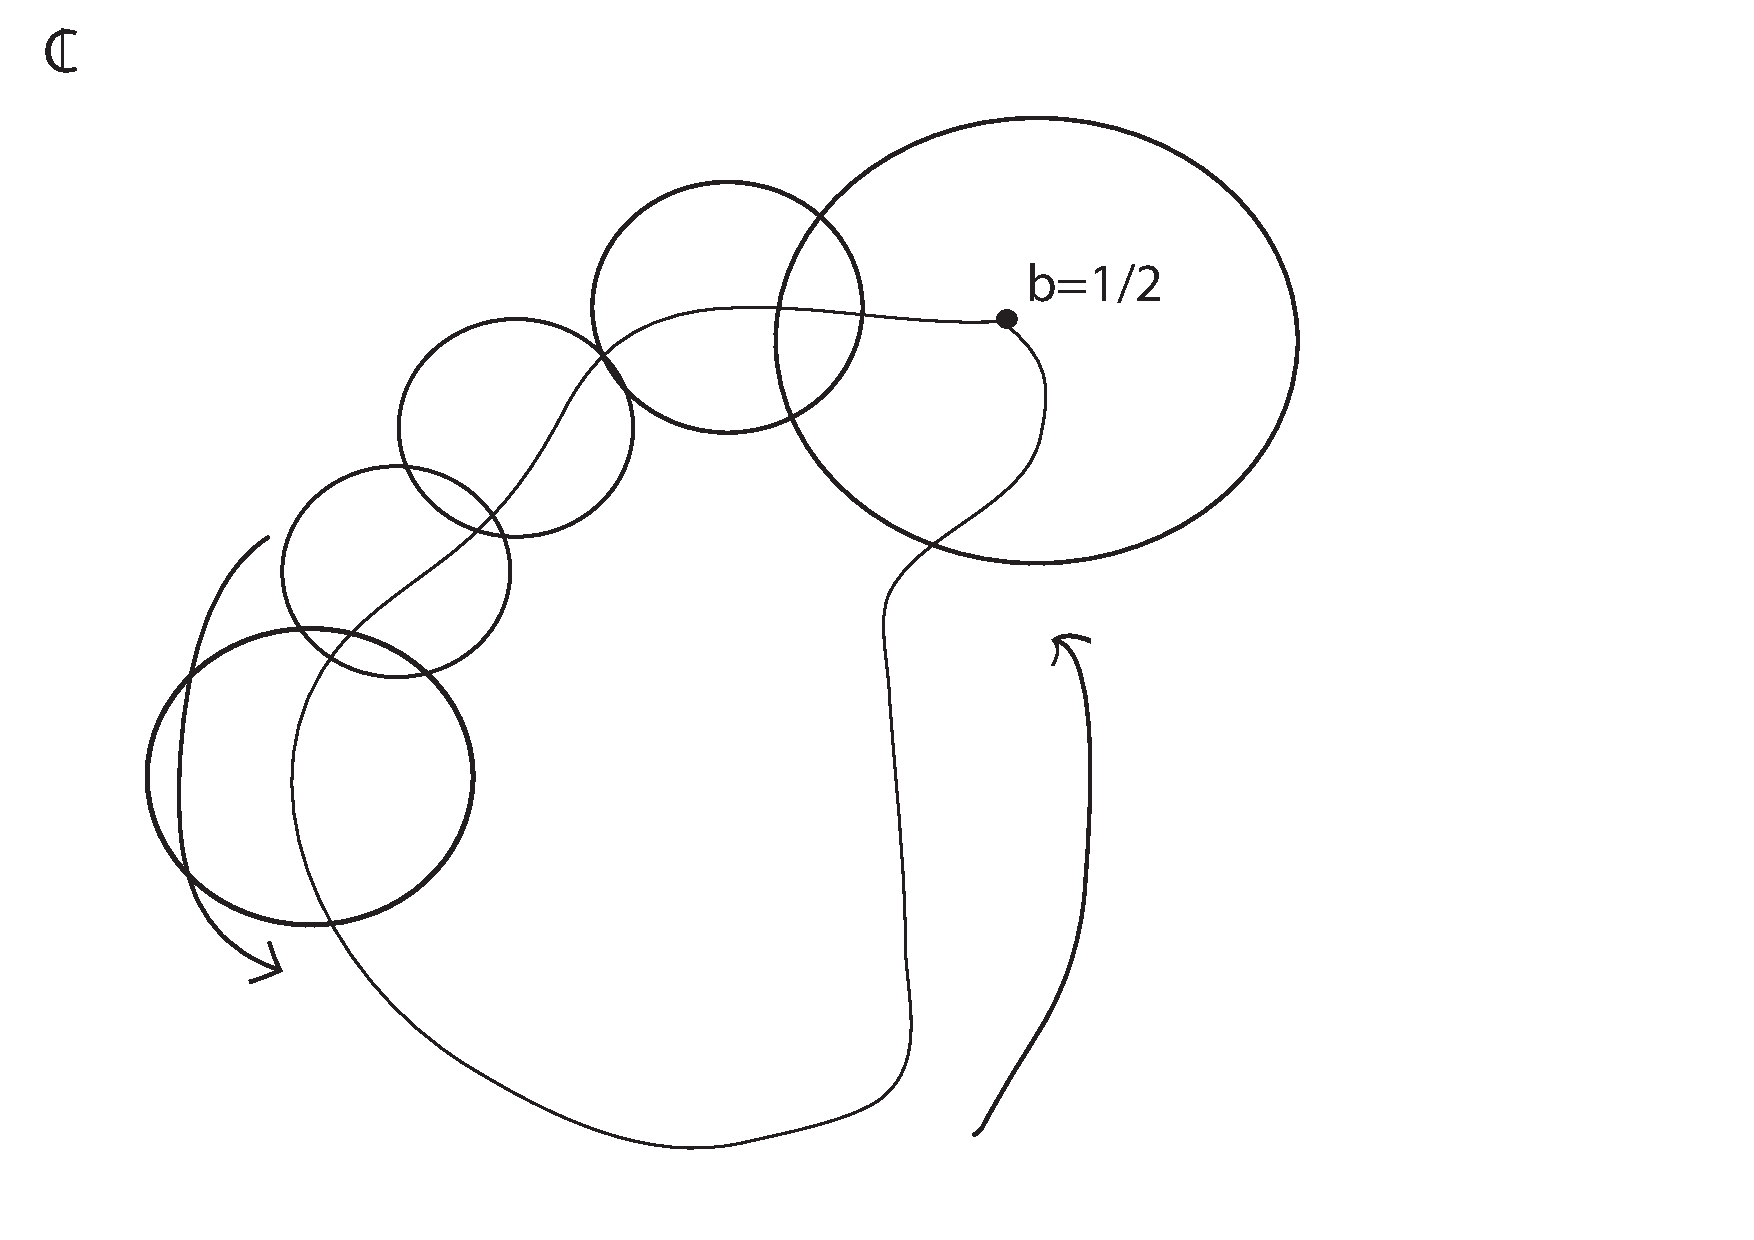
\includegraphics[width=10cm]{abstract-dibujo1.pdf}\\
  \caption{Continuaci\'on anal\'itica}
\end{figure}




El grupo de monodrom\'ia nos da informaci\'on importante  de la ecuaci\'on diferencial. En general hallar la monodrom\'ia relativa a una ecuaci\'on diferencial no es una tarea sencilla . %Dado este hecho,   
Nos proponemos  hallar y dar de manera expl\'icita %la monodrom\'ia y
el grupo de monodrom\'ia de la ecuaci\'on diferencial hipergeom\'etrica.

 $$x(1-x)\frac{d^{2}u}{dx^{2}} +  \lbrace c- (a+b+1 )x \rbrace \frac{du}{dx} - abu=0 $$

 Por medio de una combinaci\'on de t\'ecnicas recopiladas de numerosos textos (de manera particular en \cite{gausspainleve}), adem\'as de dar un conjunto de soluciones para esta ecuaci\'on en el punto $b=\frac{1}{2}$.\\



El grupo de monodrom\'ia de la ecuaci\'on hipergeom\'etrica tiene una estructura de grupo de Schottky cuando tomamos los exponentes puramente imaginarios, los exponentes dados por

$$1-c = i\theta_{0}, c-a-b = i\theta_{1},a-b=i\theta_{2} $$

Con $\theta_{i} > 0$.

Podemos describir la monodrom\'ia de la ecuaci\'on diferencial hipergeom\'etrica por medio de reflexiones respecto a c\'irculos $C(c,r)$ (donde $c$ es real)

$$\psi (c,r):s \mapsto \frac{r^{2}}{\bar{s} -c} +c$$

Y con estas reflexiones asociarle un grupo de Schottky, todo esto siguiendo los pasos de Takashi Ichikawa y Masaaki Yoshida  en una publicaci\'on titulada "ON SCHOTTKY GROUPS ARISING FROM THE HYPERGEOMETRIC EQUATION WITH IMAGINARY EXPONENTS" (\cite{Masaaki}).

El grupo de Schottky $\Lambda_{\theta}$ asociado a la ecuaci\'on hipergeom\'etrica con exponentes imaginarios nos sirve de ejemplo en un teorema sobre grupos de isometrias del plano hiperb\'olico que act\'uan de manera discontinua en el cual se destaca su prueba casi completamente geom\'etrica propuesta en un art\'iculo de W. Fenchel y J. Nielsen llamado "ON DISCONTINOUS GROUPS OF ISOMETRIC TRANSFORMATIONS OF THE NON-EUCLIDIAN PLANE" publicado en el año de 1948 (\cite{Nielsen}), aunque dado que tenemos 3 parametros $\theta_{1},\theta_{2},\theta_{3}$, en realidad hemos dado muchos ejemplos que cumplen de igual manera este prop\'osito.


Para obtener este resultado usamos la noci\'on de grupo \textit{elemental} que definimos enseguida.

\begin{defn}
\label{def:elemental}
Un grupo es elemental si su conjunto l\'imite esta formado a lo m\'as por dos puntos
\end{defn}

La caracteristica que realmente es de \'interes para nosotros es que un grupo sea NO-elemental, dicho grupo es por lo tanto un grupo cuyo conjunto l\'imite esta formado por  mas de dos puntos.
En \cite{Nielsen} tenemos la siguiente definici\'on;

\begin{defn}
\label{def:discontinuo2}
Un grupo $G$ se dice discontinuo en un punto $x \in \mathbb{D}$ si $x$ no es un punto de acumulaci\'on de la clase $Gx$
\end{defn}

Nuestro objetivo es encontrar ejemplos de grupos que actuen de manera discontinua en $\mathbb{D}$ y verificar en ellos las condiciones del teorema de Nielsen. Los grupos de Schottky que hallamos son discretos y adem\'as son No-elementales estas caracteristicas implican que se cumple en $\mathbb{D}$ la siguiente definici\'on;



\begin{defn}
\label{def:discontinuo1}
Sea $X$ un espacio topologico arbitrario y $G$ un grupo de homeomorfismos de $X$ en $X$. Se dice que $G$ act\'ua discontinuamente en $X$ si y solo si para cada subconjunto compacto $K$ de $X$ se tiene,

$$g(K) \cap K = \emptyset $$

Excepto para un n\'umero finito de $g$'s en $G$
\end{defn}

Los ejemplos que encontramos satisfacen lo que deseamos gracias a un teorema que podemos encontrar en  \cite{Beardon}, pero tambi\'en gracias a que \ref{def:discontinuo1} implica \ref{def:discontinuo2}, de esta manera sabemos de antemano que nuestros grupos act\'uan de manera discontinua pero tambi\'en nos interesa indagar las condiciones que el teorema de Nielsen requiere y deducir algunas propiedades ya que la demostraci\'on de este teorema en \cite{Nielsen} aclara el comportamiento geom\'etrico de los grupos de transformaciones hiperb\'olicas.

El cap\'itulo 1 y 2 nos dan las bases para el desarrollo de este trabajo. El cap\'itulo 1 esta basado en las definiciones necesarias como continuación anal\'itica , grupos Klenianos y de Schottky as\'i como una  introducción de la ecuación diferencial hipergeom\'etrica.

En el cap\'itulo 2 hablamos de la monodrom\'ia en general, el esquema de Riemann, calculamos la monodrom\'ia de la ecuaci\'on hipergemo\'etrica y hallamos el grupo de monodrom\'ia con las soluciones dadas por la serie hipergeom\'etrica.


En el cap\'itulo 3 construimos el grupo de schottky asociado al grupo de monodrom\'ia a trav\'es de los dominios fundamentales dados en (\cite{Masaaki})dicho grupo generado por reflexiones nos servira como ejemplo para el teorema principal.

En el cap\'itulo 4 probamos el teorema de Nielsen en 2 partes, la primera parte se prueba de manera sencilla bajo el supuesto de que en el grupo $G<PSL(2,\mathbb{R})$ existen elementos el\'ipticos, la segunda parte supone que no existen elementos el\'ipticos en el grupo y se utilizan 5 lemas para probar el teorema, estos lemas destacan mayormente por sus demostraciones puramente geom\'etricas asi como la demostraci\'on del teorema, al final probamos que el grupo de Schottky encontrado aplica en el teorema de Nielsen.      



\end{resumen}


%\begin{laburpena}        %this creates the heading for the abstract page
%\selectlanguage{basque}
% Jarri zure laburpena hemen.
%\end{laburpena}

%\end{abstractlongs}


% ----------------------------------------------------------------------


%% Thesis Acknowledgements ------------------------------------------------


% Opening of the acknowledgements

%Sort version
%this creates the heading for the acknowlegments
\begin{acknowledgements}      
%Long version
%uncommenting this line, gives a different acknowledgements heading
%\begin{acknowledgementslong} 

Lorem ipsum dolor sit amet, consectetur adipiscing elit. Ut ultrices egestas nunc, venenatis rhoncus elit fermentum non. Pellentesque gravida nulla vitae ipsum lobortis ullamcorper. Ut adipiscing, tellus in egestas mattis, enim metus pretium erat, ac tempor dolor neque placerat nulla. Nullam nec ligula eu ipsum pharetra semper a in magna. Integer ut tortor quis nisi fringilla euismod eu ac ipsum. Pellentesque sodales consectetur erat eget rutrum. Proin ornare dolor ut arcu aliquet vestibulum. Pellentesque laoreet tincidunt sem eget semper.

Integer interdum mattis magna ullamcorper tristique. Nullam commodo nulla eget ipsum vulputate tincidunt auctor leo aliquet. Fusce euismod sagittis ante, eu vulputate eros dictum at. Cras non euismod nunc. Nullam velit diam, consectetur sed eleifend vitae, blandit at arcu. Maecenas ut urna nec turpis lobortis commodo. Aliquam aliquet turpis id massa viverra id sollicitudin est cursus. Sed a tortor non mauris cursus imperdiet.

Integer fermentum rutrum urna at vestibulum. Vivamus ullamcorper erat in sapien dignissim pellentesque. Integer convallis fringilla dictum. In bibendum lectus eu nulla pretium volutpat. Morbi hendrerit fringilla tortor, sed gravida neque lacinia a. In risus magna, hendrerit vitae cursus ac, vehicula at eros. Aenean quis ipsum sit amet leo vestibulum cursus.

Cras placerat mattis dui quis vehicula. Nulla sit amet metus nibh, at auctor enim. Quisque congue ultricies sapien in suscipit. Fusce vitae placerat ante. Praesent aliquet urna ac elit consequat nec mattis augue faucibus. Nunc et sapien vel felis mollis sodales. Aenean molestie nulla vestibulum nisi fringilla vel euismod dolor tristique. Aenean fermentum, dolor eget tincidunt faucibus, risus lorem feugiat elit, sagittis malesuada eros ligula in odio. Pellentesque ac libero lobortis justo bibendum laoreet. Cras egestas lorem eget ligula dignissim sollicitudin. Vestibulum sit amet augue ultrices erat faucibus vestibulum. Aenean tincidunt faucibus leo, nec auctor diam bibendum a. Sed varius, mauris in pellentesque scelerisque, nisl ligula viverra erat, in eleifend tellus enim ac magna. Pellentesque quis est risus. Cras mollis feugiat auctor. Proin ac eros vitae nulla gravida varius.

Morbi at augue sapien. Duis tempus quam vitae velit interdum ultricies. Vivamus laoreet lacinia elit sit amet vehicula. Ut congue diam ac magna hendrerit sed fermentum justo lacinia. Curabitur vel odio neque, quis consequat mi. Proin lobortis justo quis enim fermentum accumsan sagittis ipsum imperdiet. Proin sem felis, laoreet placerat egestas id, fringilla id mauris. Pellentesque a nisi sit amet leo consectetur gravida nec et dui. Curabitur quis hendrerit augue. Etiam sed dui nec tortor convallis fringilla. Proin tempor mattis diam nec egestas. Quisque condimentum elementum lacus ac porta. Vivamus congue, odio eu ullamcorper elementum, leo turpis tempus sem, at condimentum dolor quam eu nunc. Pellentesque eget risus ac velit aliquam sollicitudin sed et ipsum.

Donec nulla enim, scelerisque quis dignissim ut, vehicula sit amet felis. Ut tristique pulvinar aliquet. Proin vitae odio nibh. Sed est dolor, malesuada et lobortis vitae, tempor quis tellus. Proin mollis lacus eget arcu tempor vitae bibendum nisi adipiscing. In sollicitudin pretium dapibus. Sed accumsan imperdiet diam quis pellentesque.

Sed in lacinia lectus. Nullam ac magna in erat blandit posuere nec nec ante. Pellentesque habitant morbi tristique senectus et netus et malesuada fames ac turpis egestas. Maecenas ipsum neque, fringilla sed sodales id, scelerisque et erat. Morbi placerat mauris vel elit ultricies sed molestie ipsum faucibus. Nunc vel sem orci, ac placerat justo. Nulla varius nisi mauris. Vivamus sed ligula felis, ac mattis purus. Vivamus felis nibh, bibendum et aliquam sed, feugiat a elit. Morbi imperdiet libero vitae lacus viverra tempus. Praesent ultricies fermentum urna eget varius. Nunc blandit, augue eget vehicula venenatis, ligula eros posuere tellus, non sollicitudin tortor velit quis augue. Nulla rhoncus fringilla dolor, vel cursus ligula varius id. Vestibulum et eros eros, ut euismod elit. Praesent placerat libero sed lorem mollis sed cursus erat laoreet.

Suspendisse in fermentum nulla. Donec blandit ultricies felis, non suscipit turpis sagittis eget. Donec eget enim in erat auctor lobortis eu sagittis mauris. Aliquam vitae nibh nisi. Integer nulla erat, feugiat quis vulputate vel, vulputate id erat. Morbi dolor dui, volutpat congue fermentum tempus, rutrum et quam. Vivamus aliquam, sapien in ultrices dictum, tortor tellus dictum justo, eu viverra velit tellus congue nibh. Suspendisse potenti. Nullam at massa id leo sollicitudin ultricies ut et nibh. Vivamus fermentum pellentesque ante et lobortis. Etiam eros justo, rutrum at varius et, porttitor ac lorem. Aenean viverra, mauris eget imperdiet aliquet, risus quam tincidunt risus, quis elementum enim diam a ipsum. Ut et arcu nunc, a viverra mi. Nullam egestas lectus vel ipsum sodales eget consectetur metus facilisis. Proin egestas magna sed felis mattis ultrices.

Morbi a lectus vitae lacus malesuada tincidunt. Vestibulum eu quam justo. Integer hendrerit posuere augue, in fringilla nulla feugiat ut. Fusce vel libero sed tellus posuere molestie in sed justo. Nunc orci magna, aliquam id dictum sit amet, bibendum vestibulum augue. Maecenas luctus ultricies elit, et aliquet justo rutrum sed. Proin mauris dui, cursus quis tempus non, rhoncus nec ante. Lorem ipsum dolor sit amet, consectetur adipiscing elit.

Fusce ac nunc non felis fermentum ultrices. Curabitur nibh felis, convallis id consequat rhoncus, elementum sodales ipsum. In hac habitasse platea dictumst. In quis nulla eu sapien mattis cursus nec semper leo. Maecenas sagittis viverra quam, vel sodales elit placerat et. Sed condimentum ultricies mattis. Pellentesque scelerisque convallis lobortis. In tempus lorem nec lorem blandit sodales. 


\begin{flushright}
\textit{Eskerrik asko,}

Your name

% Moth and year
\monthname \ \the\year



% Signature figure

%\begin{figure}[htbp!]
%\end{figure}
%\includegraphics{signature}%



\end{flushright}



%Closing of the acknowledgements
%Sort version
\end{acknowledgements}
% Long version
%\end{acknowledgementslong}

% ------------------------------------------------------------------------




% As abstract contains various languages we set the main language again
\selectlanguage{spanish}


%: ----------------------- contents ------------------------

\setcounter{secnumdepth}{5} % organisational level that receives a numbers
\setcounter{tocdepth}{5}    % print table of contents for level 3


%%You can also add extra lines to the ToC or to force extra unnumbered section headings to be included. For example, if you wanted to add an entry called Preface, and you didn't want the Preface to be numbered, you'd use these commands:
%\ subsection*{Preface}
%\addcontentsline{toc}{subsection}{Preface}

\tableofcontents            % print the table of contents
% levels are: 0 - chapter, 1 - section, 2 - subsection, 3 - subsection

%: ----------------------- list of figures/tables ------------------------

\listoffigures	% print list of figures
%\listoftables  % print list of tables


%: ----------------------- glossary ------------------------

% Tie in external source file for definitions: /0_frontmatter/glossary.tex
% Glossary entries can also be defined in the main text. See glossary.tex
%% this file is called up by thesis.tex
% content in this file will be fed into the main document

% Glossary entries are defined with the command \nomenclature{1}{2}
% 1 = Entry name, e.g. abbreviation; 2 = Explanation
% You can place all explanations in this separate file or declare them in the middle of the text. Either way they will be collected in the glossary.

% required to print nomenclature name to page header
\markboth{\MakeUppercase{\nomname}}{\MakeUppercase{\nomname}}

% ----------------------- contents from here ------------------------
%

%
%
%% acronyms


\nomenclature{IP}{Internet Protocol}







%\begin{multicols}{2} % \begin{multicols}{#columns}[header text][space]
%\begin{footnotesize} % scriptsize(7) < footnotesize(8) < small (9) < normal (10)

%\printnomenclature[1.5cm] % [] = distance between entry and description

\printnomenclature % [] = distance between entry and description

\label{sec:glossary} % target name for links to glossary

%\end{footnotesize}
%\end{multicols}




%: --------------------------------------------------------------
%:                  MAIN DOCUMENT SECTION
% --------------------------------------------------------------

% the main text starts here with the introduction, 1st chapter,...
\mainmatter

%\renewcommand{\chaptername}{A} % uncomment to print only "1" not "Chapter 1"
\pagestyle{fancy}

%: ----------------------- subdocuments ------------------------

% Parts of the thesis are included below. Rename the files as required.
% But take care that the paths match. You can also change the order of appearance by moving the include commands.

%: ----------------------- introduction ------------------------
% introduction

% this file is called up by thesis.tex
% content in this file will be fed into the main document

%: ----------------------- introduction file header -----------------------


%\begin{savequote}[50mm]
%The beginning is the most important part of the work.
%\qauthor{Plato}
%\end{savequote}




\chapter{Preliminares}
\label{cha:Introduction}

% the code below specifies where the figures are stored
%\ifpdf
   % \graphicspath{{1_introduction/figures/PNG/}{1_introduction/figures/PDF/}{1_introduction/figures/}}
%\else
 %   \graphicspath{{1_introduction/figures/EPS/}{1_introduction/figures/}}
%\fi


%-------------------------------------------------------------------------

%\cite{turing1950computing}




% ----------------------------------------------------------------------

\section{La ecuaci\'on diferencial hipergeom\'etrica y sus soluciones  } \label{sec:sol_ec_hip}

Consideremos la siguiente serie :

$$F(a,b,c;x)= \sum_{n=0}^{\infty } \frac{(a)_{n} (b)_{n}}{(c)_{n}(1)_{n}} x^{n}$$

En donde $x$ es una variable compleja , $(\alpha)_{n} = \alpha (\alpha +1)(\alpha +2)\cdots (\alpha +n-1)$, %cuando n= 0? %

y $c \neq 0, -1, -2,...$. Esta serie es la llamada serie hipergeométrica.  El coeficiente $n$-\'esimo de esta serie al que llamaremos $A_{n}$ esta dado por $$A_{n}=\frac{a(a+1)\cdots (a+n-1) \cdot b(b+1)\cdots(b +n -1) }{c(c+1)\cdots (c+n-1) \cdot 1 (1+1) \cdots (n)}$$ De esta igualdad obtenemos:

\begin{equation}
\frac{A_{n+1}}{A_{n}}= \frac{(a+n)(b+n)}{(c+n)(1+n)}
\end{equation}

Usando el criterio del cociente podemos notar que el radio de convergencia de esta serie es 1, cuando $a$ o $b$ son negativos  la serie es finita. De cualquier modo tenemos que dicha serie define una funci\'on holomorfa en $x$ en al menos el disco de radio 1 centrado en 0 y tambi\'en es holomorfa en $(a,b,c)$ si $c \neq 0, -1, -2,...$ \\

Nuestro inter\'es por la serie definida anteriormente viene del hecho que dicha serie es una soluci\'on de la ecuaci\'on diferencial hipergeom\'etrica

$$ x(1-x)\frac{d^{2}u}{dx^{2}} + \lbrace c- (a+b+1)x \rbrace \frac{du}{dx} -abu=0 $$

 A la cual denotamos $E(a,b,c;x)$ y la referimos como la serie hipergeom\'etrica con par\'ametros $(a,b,c)$. Para ver que $F(a,b,c;x)$ es una soluci\'on de $E(a,b,c)$ procedemos como Euler e introducimos el operador $ D = x \frac{d}{dx}$, a continuaci\'on  enunciamos algunas  propiedades que son \'utiles:


\begin{enumerate}
\item $Dx^{n}= nx^{n}$
\item $f(D)x^{n}=f(n)x^{n}$ donde $f$ es un polinomio de coeficientes constantes
\end{enumerate}

La propiedad n\'umero 1 es clara de la definici\'on, para la propiedad n\'umero 2 debemos dejar en claro como funciona el operador $D^{n}$ al aplicarlo a $x^{n}$. Cuando $n=2$ tenemos que $D^{2} x^{n} = x\frac{d}{dx} (x\frac{d}{dx} (x^{n}) )= x\frac{d}{dx}(x \cdot nx^{n-1})=x\frac{d}{dx} (nx^{n} ) = x\cdot n^{2}x^{n-1}=n^{2}x^{n}$, en general se tiene por un proceso an\'alogo al anterior que $D^{m}x^{n}=n^{m}x^{n}$.Sea

$$ f(x)= \sum_{i=0}^{n} a_{i}x^{i} $$

Donde $a_{n} \neq 0$, un polinomio de grado n y por $f(D)$ entendemos el operador $$f(D) = \sum_{i=0}^{n} a_{i}D^{i}$$

Entendiendo $D^{i}$ como la composici\'on del operador $D$ $i$-veces consigo mismo. Aplicamos este operador a $x^{n}$ y obtenemos

$$f(D)x^{n}=(\sum_{i=0}^{n}a_{i}D^{i}) x^{n} = \sum_{i=0}^{n}a_{i} D^{i}( x^{n}) = \sum_{i=0}^{n}a_{i}n^{i}x^{n} = f(n)x^{n}   $$


Gracias a este operador $D$ podemos escribir la ecuaci\'on diferencial hipergeom\'etrica en t\'erminos de dicho operador para obtener;

$$E(a,b,c): [(a+D)(b+D)- (c+D)(1+D)\frac{1}{x}]u=0$$

Con esta nueva presentaci\'on verificamos que la serie $F(a,b,c;x)$ es una soluci\'on de dicha ecuaci\'on. \\

Podemos escribir

$$F(a,b,c;x)= \sum_{n=0}^{\infty } \frac{(a)_{n} (b)_{n}}{(c)_{n}(1)_{n}} x^{n} = \sum A_{n} x^{n}$$

Y evaluamos

$$[(a+D)(b+D)- (c+D)(1+D)\frac{1}{x}] \sum A_{n}x^{n}$$
$$= \sum [(a+D)(b+D)A_{n}x^{n}- (c+D)(1+D)A_{n}x^{n-1}]$$
$$= \sum [(a+n)(b+n)A_{n}x^{n}- (c+n-1)(1+n-1)A_{n}x^{n-1}]$$
$$= \sum [(a+n)(b+n)A_{n}x^{n}- (c+n)(1+n)A_{n}x^{n}]=0$$


La \'ultima igualdad se da gracias a que obtenemos una serie telesc\'opica. Esta serie tiene singularidades en $0,1$ e $\infty$, nuestro objetivo ahora es encontrar soluciones en los puntos singulares como hicimos anteriormente con $x=0$. Denotaremos  a la soluci\'on  $F(a,b,c;x)$ como $f_{0}(x;0)$. \\

Queremos hallar otra soluci\'on en $x=0$ pero para esto necesitamos calcular la aplicaci\'on del operador $D$ al t\'ermino $x^{s} u$;

$$D(x^{s}u)= sx^{s}u + x^{s}Du = x^{s}(s +D)u$$

esto es $Dx^{s}= x^{s} (s + D)$, con este c\'alculo podemos obtener una expresi\'on equivalente para

$$[(a+D)(b+D) - (c+d)(1+d) \frac{1}{x}] x^{1-c} $$

La expresi\'on anterior es equivalente a

$$x^{1-c}[(a+1-c+D)(b+1-c+D)-(1+D)(2-c+D)\frac{1}{x}]$$

y esto nos dice que

$$x^{1-c} F(a+1-c,b+1-c,2-c:x) $$

Es tambi\'en una soluci\'on de $E(a,b,c)$. Aunque la serie anterior esta definida solamente cuando $2-c$ no es un entero negativo o cero (cuando es $c=1$ la serie  coincide con $F(a,b,c;x)$) esto no afecta nuestra soluci\'on ya que tomamos $1-c \in i\mathbb{R}$ en cuyo caso siempre esta definida. A esta ultima soluci\'on la denotamos por $f_{0}(x;1-c)$.

Queremos hallar tambi\'en soluciones alrededor del punto singular $x=1$, llevamos a cabo una transformaci\'on de la variable $x$ en $1-x$ abusando de la notaci\'on, y verificamos como luce ahora

$$E(a,b,c)=x(1-x) \frac{d^{2}u}{dx^{2}} + \lbrace c- (a+b+1)x \rbrace \frac{du}{dx} -abu$$

 Bajo esta transformaci\'on el primero y el tercer t\'ermino no cambian, pero el segundo t\'ermino ahora es

$$-\lbrace  c- (a+b+1)(1-x)\rbrace = a+b+1-c-(a+b+1)x $$

Entonces podemos notar que la ecuaci\'on transformada es de nuevo la ecuaci\'on hipergeom\'etrica con par\'ametros $ (a,b,a+b+1-c)$ y a menos que $c-a-b$ sea entero obtenemos como antes dos soluciones pero ahora alrededor de $x=1$

$$F(a,b,a+b+1-c;1-x), \ \ (1-x)^{c-a-b}F(c-a,c-b,c+1-a-b;1-x)$$

En nuestro caso tomamos $c-a-b \in i\mathbb{R} $ por lo que las soluciones anteriores siempre estan definidas en su radio de convergencia. A las soluciones anteriores las denotamos $f_{1}(x;0) $ y $f_{1}(x;c-a-b)$ respectivamente.

\section{Continuaci\'on anal\'itica}

La continuaci\'on anal\'itica nos da una forma de extender el dominio sobre el cual una funci\'on anal\'itica esta definida, si tomamos la serie de potencias,

\begin{equation} \label{serie de potencias}
 f(z) = \sum_{k=0}^{\infty} a_{k} (z-z_{0})^{k}
\end{equation}


Esta serie de potencias generalmente es v\'alida en un radio de convergencia dado, en ciertos casos $f$ tiene una serie de potencias que es v\'alida mas all\'a del radio de convergencia esperado, y esta serie de potencias puede servir para definir la funci\'on $f$ fuera de su dominio de definici\'on original.

Sean $f_{1},f_{2}$ funciones anal\'iticas en dominios $\Lambda_{1},\Lambda_{2}$ respectivamente, supongamos adem\'as que la intersecci\'on $\Lambda_{1} \cap \Lambda_{2}$ es no vac\'ia y $f_{1}=f_{2}$ en $\Lambda_{1} \cap \Lambda_{2}$, en este caso llamamos a $f_{2}$ la continuaci\'on anal\'itica de $f_{1}$ a $\Lambda_{2}$ y viceversa, A\'un m\'as si dicha extensi\'on existe es \'unica.

Para dar una definici\'on formal supongamos que $f$ es anal\'itica en una vecindad $U_{z_{0}}$ de $z_{0}$ y $\gamma: [a,b] \rightarrow D $ un camino en $D$ basado en $z_{0}$.


\begin{defn}
Sea $f^{*}:[a,b] \rightarrow \mathbb{C}$  una funci\'on continua con las siguientes propiedades:
\begin{enumerate}
\item $f^{*}(t) =f (\gamma (t))$  para $t$ cercano a $a$ (en $[a,b]$).
\item Para cada $t' \in [a,b]$, hay una funci\'on $h_{t'}(z)$ anal\'itica en un disco $D_{t'}$ sobre $\gamma (t')$ con $h_{t'}(\gamma (t)) = f^{*}(t)$ para $t$ cercano a $t'$ en $[a,b]$
\end{enumerate}
Si tal $f^{*}$ existe esto nos define $h_{t'}(z)$. Esta es la continuaci\'on anal\'itica de $f$ a $t'$. Es una funci\'on anal\'itica en alguna vecindad de $\gamma (t')$. Nos interesa realmente la funci\'on $h_{b}(z)$ anal\'itica en una vecindad de $\gamma (b)$. Le llamamos $f_{\gamma} (z) = f_{\gamma}$, la continuaci\'on anal\'itica de $f$ (a lo largo de $\gamma$).
\end{defn}

Nuestro inter\'es en la continuaci\'on anal\'itica radica en la manera de hallar el grupo de monodrom\'ia, si tenemos un punto $a \in \mathbb{C}$ y una vecindad $U_{a}$ en la cual tenemos un conjunto de soluciones linealmente independientes, la monodrom\'ia que mas adelante analizamos con m\'as detalle tiene relaci\'on con la continuaci\'on anal\'itica de las soluciones de una ecuaci\'on diferencial a traves de lazos anclados en $a$ y sus clases (es decir el grupo fundamental) y las matrices que relacionan a estas soluciones.

Cuando tratamos con la ecuaci\'on hipergeom\'etrica, el teorema fundamental de Cauchy nos dice que para cada punto $x_{0} \neq 0,1$ existen dos soluciones holomorfas linealmente independientes alrededor de $x_{0}$, en otras palabras, el conjunto de estas soluciones forman un espacio lineal bidimensional sobre $\mathbb{C}$. Cualquiera de estas soluciones se puede continuar anal\'iticamente a lo largo de cualquier lazo en $\mathbb{C} - \lbrace0,1 \rbrace$. Las soluciones en general no son univaluadas. Si $\gamma$ es un lazo anclado en $x_{0}$ y $u_{1}$ una soluci\'on no cero, y $u_{2}$ otra soluci\'on que no es m\'ultiplo constante de $u_{1}$ y sean $\gamma^{*} u_{1}$ y $\gamma^{*} u_{2}$ las continuaciones anal\'iticas a trav\'es de $\gamma$, como $\gamma^{*} u_{1},\gamma^{*} u_{2}$ siguen siendo soluciones linealmente independientes se tiene que existe una matriz $M(\gamma) \in GL(2,\mathbb{C})$ que relaciona a estas soluciones, esta matriz se llama la matriz de conexi\'on de $(u_{1},u_{2})$ a lo largo de $\gamma$.

\begin{figure}[h]
  \centering
  % Requires \usepackage{graphicx}
  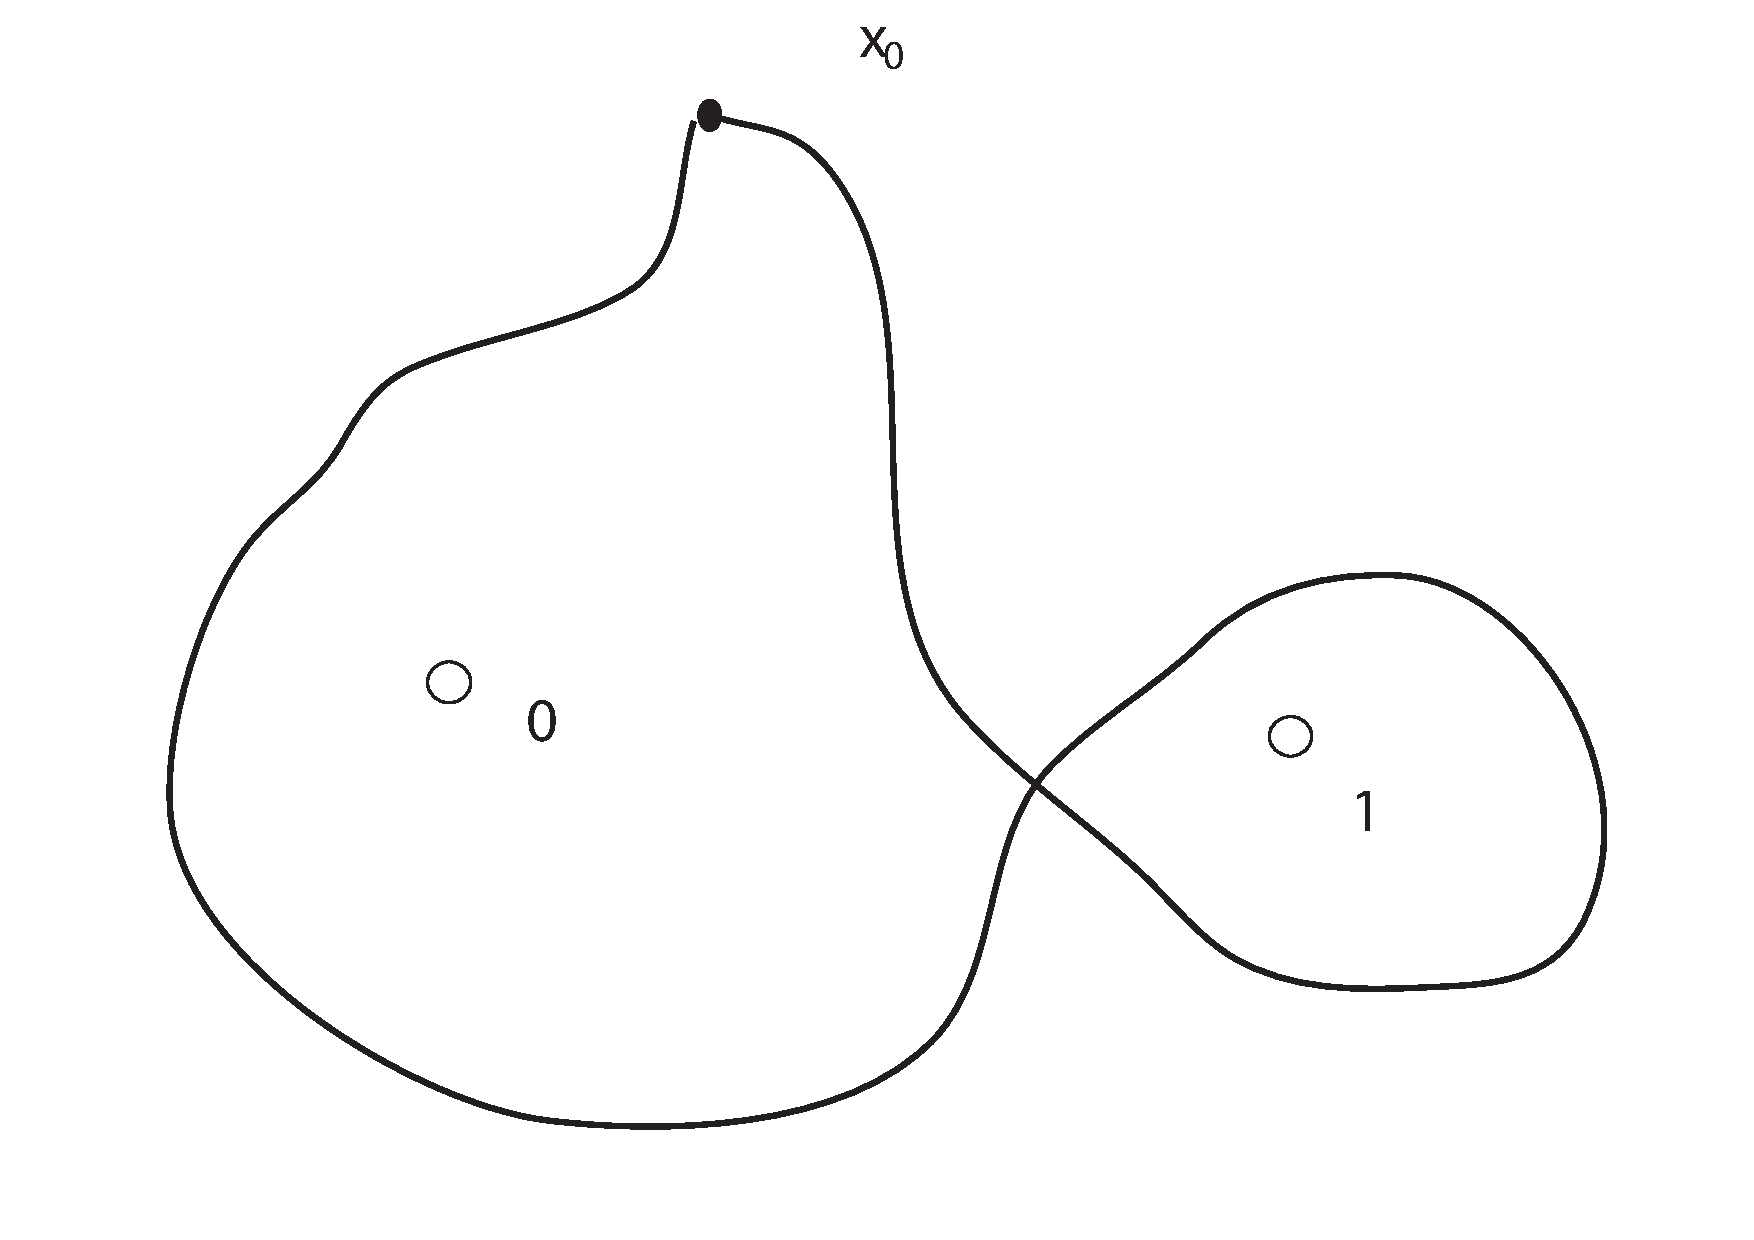
\includegraphics[width=8cm]{continuacion-analitica.pdf}\\
  \caption{Lazo anclado en un punto en $\mathbb{C}- \lbrace 0,1 \rbrace$ }\label{continuacion-analitica}
\end{figure}


Las matrices de conexi\'on juegan un papel fundamental en nuestra b\'usqueda del grupo de monodrom\'ia.

\section{Grupos Klenianos y grupos de Schotkky}

De entre los ejemplos de subgrupos discretos de isometr\'ias hiperb\'olicas conocidos, los grupos de Schotkky son ejemplos cl\'asicos de estos, al ser nuestro objetivo dar un ejemplo de un grupo de Schotkky tenemos la obligaci\'on de dar una definici\'on e introducir brevemente algunos resultados interesantes.

\begin{defn}
Un grupo de Schotkky  es un grupo generado por transformaciones de Möbius $g_{1},..g_{k},k \geq 1$ junto con una colecci\'on de pares de regiones disjuntas en $\widehat{\mathbb{C}}$, digamos $C_{1},B_{1},..,C_{k},B_{k}$, acotadas por curvas de jordan,tal que $g_{i} (C_{i}) = \widehat{\mathbb{C}} - \bar{B_{i}}$ para toda $i=1,..k.$, el conjunto $g_{1},..,g_{k}$ es llamado un conjunto de generadores Schotkky, los dominios $C_{i},B_{i}$ un conjunto fundamental de dominios y el entero $k$ el g\'enero del grupo de Schottky.
\end{defn}

Todos los grupos de Schottky son grupos finitamente generados tal que todos sus elementos no triviales son loxodr\'omicos, cuando decimos elementos no triviales nos referimos a todos excepto la identidad.

Un grupo de Schottky es cl\'asico si las curvas de jordan correspondientes a alg\'un conjunto de generadores se pueden escoger como c\'irculos.

Un grupo de Schottky tambi\'en puede ser caracterizado de la siguiente manera

\begin{thm}
Un grupo $G < PSL(2,\mathbb{C})$ es un grupo de Schottky si y solo si $G$ es finitamente generado, y un grupo Kleniano puramente loxodr\'omico que es isomorfo a un grupo libre.
\end{thm}

En nuestro caso la noci\'on de grupo de Schottky que usamos es la siguiente: Consideremos una familia de pares de 2-discos disjuntos $D_{1},..,D_{s}$ en la 2-esfera cuyas fronteras son los c\'irculos $C_{1},..,C_{s}$ y sean $\gamma_{1},..,\gamma_{s}$ inversiones en estos $s$ c\'irculos y sea $G$ el grupo generado por estas inversiones. Le llamamos a $G$ un grupo de Schottky. El subgrupo de \'indice 2 de longitud par es un grupo de Schottky cl\'asico.

El t\'ermino grupo Kleniano se utiliza para referirse a cualquier subgrupo discreto de isometr\'ias hyperb\'olicas siendo cierto o no que su regi\'on de discontinuidad sea vac\'ia.

Si el lector desea conocer todos estos conceptos en profundidad se sugiere revisar la bibliografia, especialmente \cite{Kleniangroups}, para nuestros prop\'ositos lo visto anteriormente es suficiente.


\section{Monodrom\'ia de la ecuaci\'on hipergeom\'etrica}
\label{cha:State of the Art}

% the code below specifies where the figures are stored
%\ifpdf
 %   \graphicspath{{2_state_of_the_art/figures/PNG/}{2_state_of_the_art/figures/PDF/}{2_state_of_the_art/figures/}}
%\else
 %   \graphicspath{{2_state_of_the_art/figures/EPS/}{2_state_of_the_art/figures/}}
%\fi


%-------------------------------------------------------------------------

%\cite{turing1950computing}

En este cap\'itulo presentamos conceptos b\'asicos de la teor\'ia de ecuaciones diferenciales as\'i como definiciones y teoremas que son \'utiles para calcular la monodrom\'ia de la ecuaci\'on hipergeom\'etrica, enunciamos los teoremas sin demostraci\'on. Para las demostraciones podemos dirigirnos a \cite{gausspainleve}. \\

 En el caso m\'as general podemos considerar un sistema de ecuaciones diferenciales ordinarias de primer orden.

\begin{equation} \label{sistema ecuaciones diferenciales}
\frac{du_{j}}{dz} = f_{i}(z,u) \ \ \  (j=1,..,r)
\end{equation}

Con la variable independiente $z$ y el vector de inc\'ognitas $u=(u_{1},u_{2},..,u_{r})$, donde el vector $f=(f_{1},..,f_{r})$ es holomorfo en un dominio $D \subset \mathbb{C} \times \mathbb{C}^{r}$

\begin{thm} Para cada $(a,b) \in D $ hay una soluci\'on \'unica $u$ de \ref{sistema ecuaciones diferenciales} holomorfa en una variedad de $a$, tal que
\begin{equation} \label{u(a)=b}
 u(a)=b
\end{equation}
\end{thm}

\begin{thm} Si el sistema \ref{sistema ecuaciones diferenciales} y el valor inicial \ref{u(a)=b} depende de manera holomorfa de un sistema de par\'ametros $s=(s_{1},..,s_{r})$, entonces la soluci\'on es holomorfa en $x$ y en $s$
\end{thm}

El motivo de definir un sistema de este tipo es que todo sistema de ecuaciones diferenciales ordinarias de cualquier orden, se puede reducir a un sistema del tipo \ref{sistema ecuaciones diferenciales}.


\section{Ecuaciones lineales }

Consideremos la siguiente ecuaci\'on diferencial ordinaria;

\begin{equation}
\label{eqn:sistema_ecuaciones_ordinarias}
\frac{d^{r}u}{dz^{r}} + a_{1}(z) \frac{d^{r-1}u}{dz^{r-1}} + \cdots + a_{r}(z)u=0
\end{equation}

Donde las $a_{j}'s$ son holomorfas en un dominio $D \subset \mathbb{C}$, introducimos nuevas variables;

$$u_{0}=u \ \ \, u_{i} = \frac{d^{i}u}{dz^{i}} \ \ \ (i=1,..,r-1)$$

La ecuaci\'on \ref{eqn:sistema_ecuaciones_ordinarias} se puede reescribir de la forma :

\begin{equation}
\frac{du_{i}}{dz} = \sum_{j=0}^{r-1} a_{i}^{j}(z)u_{j} \ \ \ (i=0,...,r-1)
\end{equation}


\begin{thm}Para cada punto $a \in D$ y cualesquiera complejos $b_{0},..,b_{r-1}$ hay una \'unica soluci\'on holomorfa de \ref{eqn:sistema_ecuaciones_ordinarias} tal que

$$\frac{d^{i}u}{dz^{i}}(a) = b_{i} \ \ \ \ \ i=0,..,r-1$$

Dicha soluci\'on tiene una continuaci\'on anal\'itica a lo largo de cualquier curva en $D$.
\end{thm}

Si los coeficientes de la ecuaci\'on \ref{eqn:sistema_ecuaciones_ordinarias} son holomorfos en $\lbrace z \mid 0 < |z-a|< \epsilon  \rbrace $ para alg\'un $\epsilon > 0 $ y al menos una es meromorfa y no holomorfa en $\lbrace z \mid |z-a| < \epsilon \rbrace$, entonces el punto $a$ es un punto singular de \ref{eqn:sistema_ecuaciones_ordinarias}. \\

\begin{defn} Un punto singular $a$ de \ref{eqn:sistema_ecuaciones_ordinarias} es regular si

$$(z-a)^{k}a_{k}(z), \ \ \ \ (k=1,..,r)$$

Son holomorfas en $a$.
\end{defn}

\section{Comportamiento alrededor de puntos singulares regulares}

Consideremos $z=0$ un punto singular regular de la ecuaci\'on  \ref{eqn:sistema_ecuaciones_ordinarias} (en el caso de la ecuaci\'on hipergeom\'etrica $z=0$ es un punto singular regular). Como en \ref{sec:sol_ec_hip} introducimos el operador;

$$D= z\frac{d}{dz} $$

Este operador se relaciona con $\frac{d}{dz}$ de la siguiente manera,

\begin{equation}  \label{relacion-operadores-com-alr-pun-sing}  \ z^{k}\frac{d^{k}}{dz^{k}}= D(D-1) \cdots (D-k+1) \end{equation}

Para $k \geq 1 $ se tiene

$$ z^{r} \lbrace \frac{d^{r}}{dz^{r}} + a_{1}(z) \frac{d^{r-1}}{dz^{r-1}} + \cdots a_{r}(z) \rbrace \
= \sum_{k=0}^{r} z^{r-k}a_{r-k}(z)D(D-1) \cdots (D-k+1) \ $$
$$=D^{r} + \lbrace za_{1}(z) - \frac{(r-1)(r)}{2} \rbrace D^{r-1} + \cdots $$

Donde $a_{0}=1$.
La ecuaci\'on \ref{eqn:sistema_ecuaciones_ordinarias} se puede reescribir en la forma

$$ Lu=0 $$

Donde $L$ es un operador de la forma;

$$ L= \sum_{i=0}^{r} b_{i}(z) D^{r-i}$$

Donde $b_{0}(z) = 1$, y $b_{1}(z),..,b_{r}(z) $ estan dados por series convergentes. Escribimos;

\begin{equation}
  b_{i}(z)=\sum_{j=0}^{\infty} b_{ij}z^{j}, \ \  0 \leq i \leq r
\end{equation}

En particular, $b_{00}= 1, b_{0j}=0, \ \ \ (j \geq 1)$, escribiendo ;

$$ u= z^{s} \sum_{k=0}^{\infty} c_{k} z^{k}, \ \ c_{o}=1$$

Calculamos $Lz$:

$$Lz = \sum_{i=0}^{r} \sum_{j=0}^{\infty} b_{ij} z^{j} D^{r-i} \sum_{k=0}^{\infty} c_{k} z ^{s+k}$$
$$= \sum_{k=0}^{\infty} \sum_{j=0}^{\infty} \sum_{i=0}^{r} b_{ij} (s+k)^{r-i}c_{k}z^{s+k+j}$$
$$= z^{s} \sum_{n=0}^{\infty} \lbrace \sum_{k=0}^{n} \sum_{i=0}^{r}  b_{i,n-k}(s+k)^{r-i}c_{k} \rbrace z^{n} $$

Y teniendo en cuenta $Dz^{\alpha} = \alpha z^{\alpha}$, escribimos;

$$f(s) = \sum_{i=0}^{r} b_{i,0}s^{r-i} = \sum_{i=0}^{r} b_{i}(0) s^{r-i}$$

\begin{defn} La ecuaci\'on algebraica

 \begin{equation} \label{eqn:ecncarac} f(s)=0 \end{equation}

Se llama la ecuaci\'on caracter\'istica en el punto singular regular $z=0$. Las ra\'ices de \ref{eqn:ecncarac}  son llamados los exponentes caracter\'isticos.
\end{defn}

\section{ Ecuaciones Fuchsianas }

\begin{lem} Una ecuaci\'on diferencial
$$ \lbrace D^{r} + b_{1}(z)D^{r-1} + \cdots + b_{r}(z)  \rbrace u =0$$

Es regular singular en $z=0$ si y solo si $b_{j}, (1 \leq j \leq r)$ son holomorfas en $z=0$
\end{lem}

La ecuaci\'on \ref{eqn:sistema_ecuaciones_ordinarias} con coeficientes racionales es $Fuchsiana$ si cada punto singular en ${\mathbb{C}}$ es regular, y si despu\'es de un cambio de variable $z$ en $t=\frac{1}{z}$, la ecuaci\'on transformada tiene un punto singular regular en $t=0$. Los exponentes de $t=0$ son llamados los exponentes de \ref{eqn:sistema_ecuaciones_ordinarias} en el infinito.

\begin{prop}[Una caracterizaci\'on de las ecuaciones $Fuchsianas$ ]
La ecuaci\'on \ref{eqn:sistema_ecuaciones_ordinarias} es $Fuchsiana$ con singularidades regulares en $z_{1},...,z_{m},z_{m+1} = \infty $ si y solo si los coeficientes tienen la siguiente forma:

$$ a_{k}(z) = \frac{p_{k}(z)}{\prod^{m}_{i=1}  (z-z_{i})^{k}}, \ \ \ \ (k=1,..,r)$$

Donde cada $p_{k}(z)$ es un polinomio de grado a lo m\'as $k(m-1)$.
\end{prop}

\begin{defn} Un esquema de $Riemann$ es una tabla donde se representan los puntos singulares $z_{1},..,z_{m+1}$ y los exponentes en $s_{i}^{1},..,s_{i}^{r}$ en $z_{i}$, el esquema de $Riemann$ de \ref{eqn:sistema_ecuaciones_ordinarias} se expresa como



\[ \left( \begin{array}{ccc}
z_{1} & ... & z_{m+1} \\
s_{1}^{1} & ... & s_{m+1}^{1} \\
... & ... & ... \\
s_{1}^{r} & ... & s_{m+1}^{r} \end{array} \right)\]

\end{defn}

\section{Esquema de Riemann de la ecuaci\'on hipergeom\'etrica}

Para nuestra ecuaci\'on hipergeom\'etrica

\begin{equation}
\label{ecuacion_hipergeometrica}
 (1-z )z \frac{d^{2}u}{dz^{2}} + \lbrace  c -(a+b+1)z \rbrace \frac{du}{dz} -abu =0
\end{equation}

Deseamos hallar el esquema de Riemann  correspondiente, esto nos sirve para hallar la monodrom\'ia mas adelante por medio de las identidades de $Gauss-Kummer$ (\cite{gausspainleve}).

Los puntos singulares de nuestra ecuaci\'on son $1,0,\infty$, y esto lo podemos ver transformando la ecuaci\'on \ref{ecuacion_hipergeometrica} a la forma est\'andar;

$$ \frac{d^{2}u}{dz} + \frac{\lbrace c-(a+b+1)z \rbrace}{z(z-1)}\frac{du}{dz} - \frac{ab}{z(z-1)}u=0$$

Y obtenemos $a_{1}(z) = \frac{c- (a+b+1)z}{z(z-1)}$ y $a_{2}(z)=\frac{-ab}{z(z-1)}$, podemos ver que los puntos singulares son $0,1$ e $\infty$ (mostramos despu\'es que $\infty$ tambi\'en es un punto singular pero consideremos por ahora que esto es cierto). Estos puntos tambi\'en son regulares como podemos verificar;

Para $z=0$
$$za_{1}(z) = z (\frac{c-(a+b+1)z}{z(1-z)})= \frac{c-(a+b+1)z}{1-z}$$

Y

$$z^{2}a_{2}(z)=z^{2} (\frac{-ab}{z(1-z)})= \frac{-abz}{1-z}$$

Y ambas son holomorfas en $z=0$, an\'alogamente verificamos que $z=1$ es un punto singular regular (El caso $z= \infty $ se deja al final). Tenemos entonces 3 puntos singulares regulares para la ecuaci\'on \ref{ecuacion_hipergeometrica}, lo que deseamos ahora es hallar los exponentes en cada punto.\\

Para $z=0$ recordemos que los exponentes son las ra\'ices de la ecuaci\'on \ref{eqn:ecncarac}, la cual esta dada en este caso por
$$f(s) = \sum_{i=0}^{2} b_{i}(0) s^{r-i} $$

Y en este caso $b_{1}(z) = za_{1}(z) -1$ y $ b_{2}(z)= z^{2}a_{2}(z)$, es decir $b_{1}(z) = \frac{c-(a+b+1)z}{1-z} -1$ y $b_{2}(z) = \frac{-ab}{1-z}$ y por tanto;

$$f(s)= s^{2} +b_{1}(0)s + b_{2}(0) = s^{2} + (c-1)s +0 $$

Cuyas ra\'ices son 0 y $c-1$. Para encontrar los exponentes en $z=1$ hacemos un proceso similar y escribimos;

$$D_{1} = (z-1)\frac{d}{dz}$$

Y se cumple la misma relaci\'on de antes entre $D_{1}$ y $\frac{d}{dz}$, luego;

$$(z-1) \lbrace \frac{d^{r}}{dz^{r}} + a_{1}(z)\frac{d^{r-1}}{dz^{r-1}}+ \cdots + a_{r}(z) \rbrace = D_{1}^{r} + \lbrace (z-1)a_{1}(z) - \frac{(r-1)(r)}{2} \rbrace D_{1}^{r-1} + \cdots $$

Si llamamos $f_{1}$ a la ecuaci\'on caracter\'istica de \ref{eqn:sistema_ecuaciones_ordinarias} en $z=1$, tenemos en este caso $b_{1}(z)= (z-1)a_{1}(z) -1$ y $ b_{2}(z) = (z-1)^{2}a_{2}(z)$ entonces;

$$ f_{1}(s) = s^{2} + b_{1}s + b_{2}(1)= s^{2} + \lbrace c-(a+b+1) +1 \rbrace s = s^{2} - (c-a-b)s $$

Cuyas ra\'ices son $0$ y $c-a-b$. Basta hallar los exponentes para $z= \infty$, hacemos una transformaci\'on $t=\frac{1}{z}$ y definimos $\theta \frac{t}{dt}$ y notamos que $D=- \theta$, obtenemos entonces;

$$z^{r} \lbrace \frac{d^{r}}{dz^{r}} + a_{1}(z) \frac{d^{r-1}}{dz^{r-1}} + \cdots +a_{r}(z) \rbrace = \sum_{k=0}^{\infty} t^{-(r-k)}a_{r-k} (\frac{1}{t})(-1)^{k} \theta (\theta +1) \cdots (\theta + k-1)$$

En nuestro caso, para $r=2$ la ecuaci\'on es

$$\theta^{2} + (1-t^{-1}a_{1}(\frac{1}{t}))\theta + t^{-2}a_{2}(\frac{1}{t}) $$

Donde $-t^{-1}a_{1}(\frac{1}{t}) = \frac{a+b+1-ct}{t-1}$ y $t^{-2}a_{2}(\frac{1}{t})= \frac{-ab}{t-1}$ de aqui vemos dado que ambas son holomorfas en $0$ que $z= \infty$ es un punto regular singular. Entonces si $f_{\infty}$ denota la ecuaci\'on caracter\'istica de \ref{ecuacion_hipergeometrica} con el cambio de variable en $t=0$, tenemos;

$$ f_{\infty}(s) = s^{2} + (-a-b)s +ab$$

Cuyas ra\'ices son $a$ y $b$, por tanto los exponentes en $z=\infty $ de \ref{ecuacion_hipergeometrica}  son $a$ y $b$. Concluimos con el esquema de $Riemann$ de la ecuaci\'on hipergeom\'etrica  esta dado por

\[ \left( \begin{array}{ccc}
0 & 1 & \infty \\
0 & 0 & a \\
1-c &c-a-b & b  \end{array} \right)\].

\section{Monodrom\'ia}

Si consideramos de nuevo la ecuaci\'on \ref{eqn:sistema_ecuaciones_ordinarias}, es posible asociarle una clase de conjugaci\'on en $GL(2,\mathbb{C})$ a la cual llamamos la monodrom\'ia de \ref{eqn:sistema_ecuaciones_ordinarias}. Consideremos el grupo fundamental $\Pi_{1} (D,b)$ donde $D$ es una vecindad en la cual los coeficientes de \ref{eqn:sistema_ecuaciones_ordinarias} son holomorfas y $b \in D$.\\

Sea $U$ una vecindad simplemente conexa de $b \in D $ y sea $\mathfrak{F}= (u_{1},..,u_{n})$ un sistema fundamental de soluciones en $U$. Si $\alpha \in \Pi_{1}(D,b)$ sea $\gamma$ un representante y $\gamma_{*} \mathfrak(F)$ la continuaci\'on anal\'itica de $\mathfrak{F} $ a lo largo de $\gamma$. El teorema de monodrom\'ia para la continuaci\'on anal\'itica (\cite{gausspainleve}) implica que $\gamma_{*} \mathfrak{F}$ depende en la clase de homotopia $\alpha$, podemos escribir entonces $\alpha_{*} \mathfrak{F}$ en lugar de $\gamma_{*} \mathfrak{F}$. Ya que \ref{eqn:sistema_ecuaciones_ordinarias} es lineal, $\alpha_{*} \mathfrak{F}$ es tambi\'en un sistema fundamental de soluciones de \ref{eqn:sistema_ecuaciones_ordinarias} en $U$ y hay una \'unica matriz invertible $M(\alpha; \mathfrak{F}) \in GL(n,\mathbb{C})$ tal que

\begin{equation} \label{relacionmatrizsisfun}
\alpha_{*} \mathfrak{F} = \mathfrak{F} M(\alpha;\mathfrak{F})
\end{equation}

Ya que $e_{*} \mathfrak{F} = \mathfrak{F}$ y $(\alpha \beta)_{*} \mathfrak{F} = \alpha_{*} (\beta_{*} \mathfrak) $ para $\alpha ,\beta \in \Pi_{1} (D,b) $ tenemos

$$M(e,\mathfrak{F}) = I , M(\alpha \beta ;\mathfrak{F}) = M(\alpha ;\mathfrak{F})M(\beta ;\mathfrak{F}) $$

Esto implica que el mapeo

$$\rho_{\mathfrak{F}}: \Pi_{1} (D,b) \rightarrow GL(n,\mathbb{C}), \alpha \mapsto M(\alpha ; \mathfrak{F}) $$

Es un homomorfismo. Llamamos a $\rho_{\mathfrak{F}}$ la representaci\'on de monodrom\'ia y a $\rho_{\mathfrak{F}}(\Pi_{1} (D,b)) \subset GL(n, \mathbb{C})$ el grupo de monodrom\'ia de \ref{eqn:sistema_ecuaciones_ordinarias} respecto al sistema fundamental de soluciones $\mathfrak{F}$. Si $\mathfrak{G}$ es otro sistema de soluciones en otro punto $a$ y denotamos tambi\'en por $\mathfrak{G}$ la continuaci\'on anal\'itica de este a lo largo de una curva que une $a$ y $b$, existe una matriz $C \in GL(n,\mathbb{C})$ tal que $\mathfrak{G} = \mathfrak{F} C$ y tenemos

$$\mathfrak{G} M(\alpha ; \mathfrak{G})=\alpha_{*} \mathfrak{G} = (\alpha_{*} \mathfrak{F}) C  = \mathfrak{F} M(\alpha ; \mathfrak{F}) C = \mathfrak{G} C^{-1 } M(\alpha ; \mathfrak{F}) C $$

Es decir

$$M(\alpha ; \mathfrak{F}) = C^{-1} M(\alpha ; \mathfrak{F} )C$$

En otras palabras

\begin{equation} \label{4.1.3relacion}
\rho_{\mathfrak{G}}(\alpha)=C^{-1} \rho_{\mathfrak{F}}(\alpha) C, para \ \alpha \in \Pi_{1} (D,b)
\end{equation}

la representaci\'on de monodrom\'ia no solo depende de la ecuaci\'on diferencial \ref{eqn:sistema_ecuaciones_ordinarias}, depende de igual manera del sistema fundamental de soluciones. Notemos que de cualquier manera que \ref{4.1.3relacion} implica que cada par de representaciones de monodrom\'ia de \ref{eqn:sistema_ecuaciones_ordinarias} son conjugadas, tal que la clase de conjugaci\'on de la representaci\'on de monodrom\'ia se determina \'unicamente por la ecuaci\'on diferencial \ref{eqn:sistema_ecuaciones_ordinarias}. A esta clase de conjugaci\'on la llamamos $La \ Monodromia$ de \ref{eqn:sistema_ecuaciones_ordinarias}. entonces el grupo de monodrom\'ia $\rho_{\mathfrak{F}} (\Pi_{1} (D,b))$ de \ref{eqn:sistema_ecuaciones_ordinarias} respecto de cualquier $\mathfrak{F} $ pertenece a la misma clase de conjugaci\'on, que tambie\'n llamamos $La \ Monodromia$ de \ref{eqn:sistema_ecuaciones_ordinarias}.


Cuando \ref{eqn:sistema_ecuaciones_ordinarias} es una ecuaci\'on diferencial fuchsiana en la esfera de Riemann con puntos singulares regulares en $p_{1},..,p_{m},p_{m+1} = \infty$, se toma $D= \mathbb{C} \backslash \lbrace p_{1},..,p_{m} \rbrace$. Para cada $j=1,..,m$, sea $U_{j}$ un disco abierto en $D \cup \lbrace p_{j}\rbrace$ centrado en $p_{j}$, y sea $\textit{l} _{j}$ un lazo en $U_{j} \backslash \lbrace p_{j} \rbrace$ con punto base $q_{j} \in U_{j} \backslash \lbrace p_{j} \rbrace$ que encierra $p_{j} $ una vez en sentido antihorario, y sea $\mathfrak{F}_{j}$ un sistema fundamental de soluciones de \ref{eqn:sistema_ecuaciones_ordinarias}  en una vecindad simplemente conexa de $b$ y $\gamma_{j}, (j=1,..,m)$  arcos con punto inicial $b$ y punto final $q_{j}$. Las matrices de conexi\'on $C_{j} \in  GL(n, \mathbb{C}), \ (j=1,..,m)$ se definen por

\begin{equation}\label{eqn:matcon1}
  \gamma_{j_{*}} \mathfrak{F} = \mathfrak{F}_{j} C_{j}
\end{equation}

\begin{prob}{Problema de matrices de conexi\'on} Para una ecuaci\'on diferencial lineal dada, sean $\mathfrak{F}, \mathfrak{F}_{j}$ y $C_{j}$ como antes. Encontrar una expresi\'on explicita de las $C_{j}$.

Las matrices de circuito $M_{j}$ alrededor de $p_{j}$ se pueden definir por

\begin{equation}\label{eqn:matcon2}
 \textit{l} _{j_{*}} \mathfrak{F}_{j} = \mathfrak{F}_{j} M_{j}
\end{equation}

\end{prob}

Ya que los generadores del grupo de monodrom\'ia respecto a $\mathfrak{F}$ estan dados por

$$C_{j}^{-1} M_{j} C_{j} ,$$

Notamos que el problema de monodrom\'ia es parte del problema de conexi\'on.



\begin{figure}[h] \label{lazos3}
  \centering
  % Requires \usepackage{graphicx}
  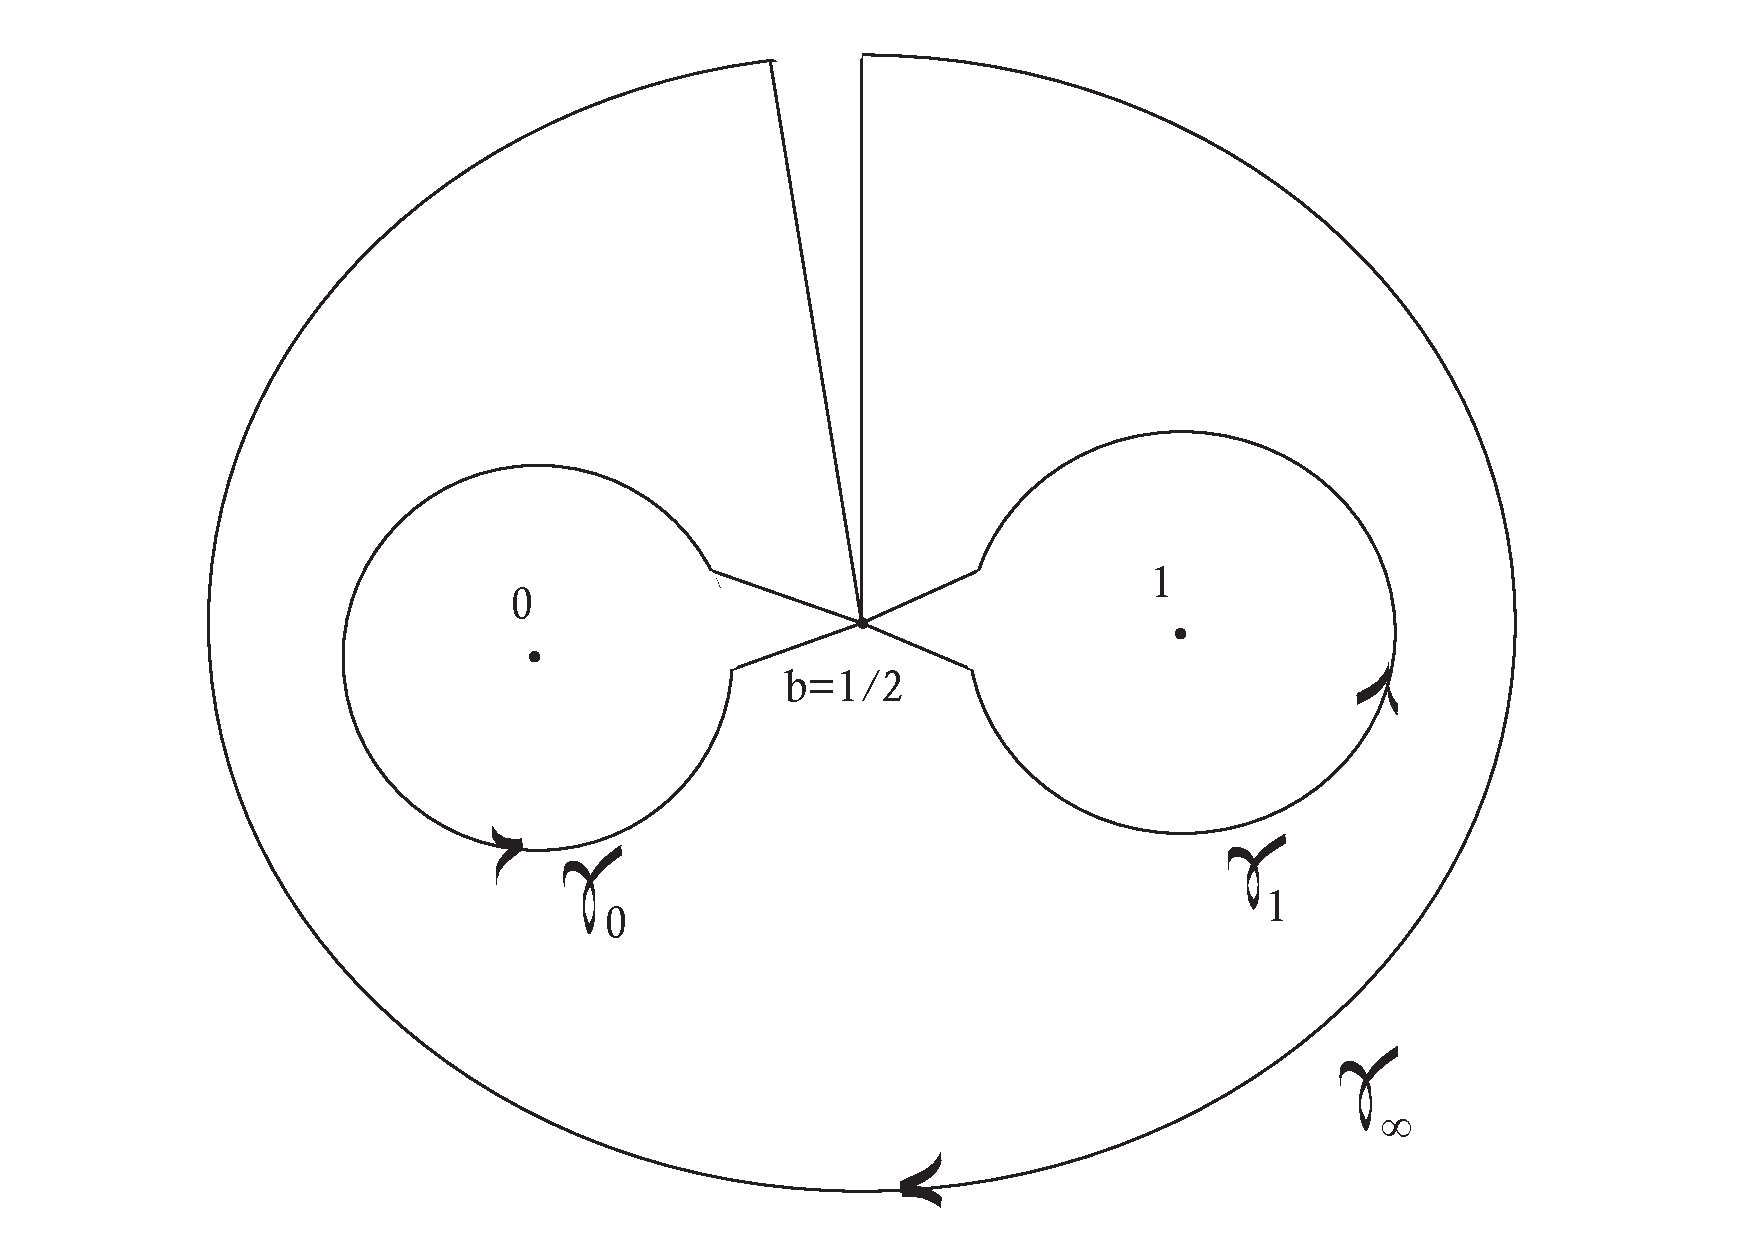
\includegraphics[width=10cm]{lazos3.pdf}
  \caption{Lazos anclados en $b=\frac{1}{2}$} \label{lazos3}
\end{figure}


El problema de hallar la monodrom\'ia respectiva a una ecuaci\'on diferencial es un problema complicado, afortunadamente existen m\'etodos que nos permiten hallar (en ciertos casos) la monodrom\'ia de la ecuaci\'on hipergeom\'etrica y tambi\'en el grupo de monodrom\'ia para soluciones particulares. En los siguientes cap\'itulos hallamos la monodrom\'ia de la ecuaci\'on hipergeom\'etrica y uno de los grupos de monodom\'ia respecto de las soluciones dadas en \ref{sec:sol_ec_hip}.


\section{Monodrom\'ia de la ecuaci\'on hipergeom\'etrica}

En esta secci\'on encontramos la monodrom\'ia de la ecuaci\'on hipergeom\'etrica a traves de su esquema de Riemann por medio de propiedades locales y la relaci\'on de Fuchs, utilizando fuertemente que la ecuaci\'on hipergeom\'etrica resulta ser irreducible.

Sea $G=\pi_{1} (D,b) $ y $\gamma_{j} \in G, (j=0,1,\infty )$, lazos en $b$. Sea $\rho: G \rightarrow GL(2,\mathbb{C}) $ una representaci\'on de monodrom\'ia del esquema de Riemann

\[ \left( \begin{array}{ccc}
0 & 1 & \infty \\
\rho_{1} & \sigma_{1} & \tau_{1} \\
\rho_{2} &\sigma_{2} & \tau_{2}  \end{array} \right)\]


Dado que 
\begin{equation}
\rho (\gamma_{1} \cdot \gamma_{0}) = \rho(\gamma_{\infty})^{-1}
\end{equation}

 ya que 
 \begin{equation}
 \gamma_{\infty}^{-1}=\gamma_{1} \gamma_{0}  y \gamma_{0}\gamma_{1}        
 \end{equation}
 
 
 es conjugado a $\gamma_{1} \gamma_{0}$, tenemos;

\begin{eqnarray} %equation
 \label{eqnarray:ecuacion1} \lbrace \varepsilon (\rho_{1}), \varepsilon (\rho_{2}) \rbrace \ conjunto \ de \ eigenvalores \ de \ \rho (\gamma_{0}) \\
 \lbrace \varepsilon (\sigma_{1}), \varepsilon (\sigma_{2}) \rbrace \  conjunto \ de \ eigenvalores \ de \ \rho (\sigma_{1}) \\
\lbrace \varepsilon(-\tau_{1}), \varepsilon (-\tau_{2}) \rbrace \  conjunto \ de \ eigenvalores \ de \ \rho (\sigma_{0} \sigma_{1})
\end{eqnarray}

Donde $\varepsilon (\cdot) = exp(2 \pi i \cdot)$. La clase de conjugaci\'on de $\rho$, es decir la monodrom\'ia de $RE(\rho,\sigma,\tau)$ esta casi determinada por los eigenvalores, y esta completamente determinada si la monodrom\'ia es irreducible.

\begin{defn}La ecuaci\'on de Riemann $RE(\rho,\sigma,\tau)$ se dice irreducible s\'i la monodrom\'ia es irreducible
\end{defn}

\begin{thm} \label{riemann-irreducible}

La ecuaci\'on de Riemann es irreducible si y solo si

$$\rho_{i} + \sigma_{j} + \tau_{k} \notin \mathbb{Z}, (i,j,k=1,2)  $$
Bajo esta condici\'on la representaci\'on $\rho $ se expresa hasta conjugaci\'on por las siguientes matrices:

$$ \rho (\gamma_{0}) \leftrightarrow  \begin{pmatrix}
 \varepsilon(\rho_{1})& 1\\
 0& \varepsilon(\rho_{2})
 \end{pmatrix}  ,\ \ \
\rho (\gamma_{1}) \leftrightarrow \begin{pmatrix}
 \varepsilon(\sigma_{1})& 0\\
 b& \varepsilon(\sigma_{2})
 \end{pmatrix}
$$

 Y el n\'umero $b$ esta dado por $b= \varepsilon(-\tau_{1}) + \varepsilon(-\tau_{2}) - \varepsilon(\rho_{1} + \sigma_{1}) - \varepsilon(\rho_{2} + \sigma_{2})$, y $\varepsilon(\cdot) =exp(2 \pi i \cdot)$. Todas las representaciones  obtenidas al intercambiar $\rho_{1},\rho_{2}$ y/o $\sigma_{1},\sigma_{2}$ son mutuamente conjugadas.

\end{thm}

En nuestro caso tenemos el esquema de Riemann;

\[ \left( \begin{array}{ccc}
0 & 1 & \infty \\
0 & 0 & a \\
1-c &c-a-b & b  \end{array} \right)\]

Y verificamos si satisface las condiciones del teorema, tenemos los siguientes casos:


\begin{enumerate}
\item 0+0+ a = a
\item 0 + c-a-b + b = c-a
\item 0 + c-a-b + a = c-b
\item 1-c + 0 + a= 1-c +a
\item 1-c + 0 + b=1-c+b
\item 1-c + c-a-b + b = 1-a
\item 0 + 0 + b = b
\item 1-c + c- a- b + a = 1-b
\end{enumerate}


 Queremos calcular $a,c-a,c-b,1-c+a,1-c+b,1-a,b,1-b$, y estamos considerando que los exponentes $ 1-c,c-a-b,a-b$ son imaginarios puros, por lo que basta probar que ninguno de los anteriores estan en $\mathbb{Z}$.

No es dif\'icil verificar que $b = \frac{1-i(\theta_{0} + \theta_{1} +\theta_{2})}{2} \notin \mathbb{R}$. Para $a$ tenemos;

$$a= \frac{1-i(\theta_{0} + \theta_{1} - \theta_{2})}{2}$$

Y podemos ver que $a \notin \mathbb{R}$ o $ a = \frac{1}{2}$  de cualquier modo $a \notin \mathbb{Z}$. Para $c-a$ se tiene;

$$c-a = \frac{1 + i (-\theta_{0} + \theta_{1} - \theta_{2})}{2}$$

Por lo que de nuevo $c-a \notin \mathbb{R}$ o $c-a = \frac{1}{2}$, y de cualquier modo $c-a \notin \mathbb{Z}$. Para $c-b$ se tiene;

$$c-b =\frac{1+i(\theta_{2} + \theta_{1} - \theta_{0})}{2} $$

Entonces $c-b \notin \mathbb{R}$ o $c-b =\frac{1}{2}$ y en cualquier caso $c-b \notin \mathbb{Z}$. Para $1-c+a$ notamos que $1-c+a= - (c-a-1 )$ y $c-a-1 = -\frac{1}{2}$ o $c-a-1 \notin \mathbb{R}$. En los casos restantes un proceso an\'alogo nos enseña que ninguno de los n\'umeros considerados esta en $\mathbb{Z}$.

Invocamos el teorema \ref{riemann-irreducible} al esquema de Riemann que hallamos para nuestra ecuaci\'on, y obtenemos que las matrices que generan la monodromia de la ecuaci\'on hipergeom\'etrica con exponentes imaginarios puros son:

$$ \rho (\gamma_{0}) \leftrightarrow  \begin{pmatrix}
 1& 1\\
 0& e^{2 \pi i (1-c)}
 \end{pmatrix}  ,\ \ \
\rho (\gamma_{1}) \leftrightarrow \begin{pmatrix}
 1& 0\\
 b& e^{2 \pi i (c-a-b)}
 \end{pmatrix}
$$

Con $b = e^{-2 \pi i a} + e^{-2 \pi i b} -1 -e^{2 \pi i (1-a-b)}$, y la monodrom\'ia de la ecuaci\'on hipergeom\'etrica es generada por $\rho (\gamma_{0}), \rho (\gamma_{1})$ en $GL(2, \mathbb{C})$.


\section{Grupo de monodrom\'ia con las soluciones dadas por la serie hipergeom\'etrica}

 En este cap\'itulo pretendemos dar a conocer el grupo de monodrom\'ia con el par de sistemas fundamentales de soluciones hallados en \ref{sec:sol_ec_hip}, utilizando las identidades de $Gauss-Kummer$. El enfoque principal en este cap\'itulo es exponer las herramientas necesarias para ese prop\'osito y los resultados principales que llevan a una expresi\'on del grupo de monodrom\'ia con los sistemas fundamentales de soluciones dadas. Los teoremas y resultados de este cap\'itulo pueden encontrarse en \cite{gausspainleve} as\'i como sus demostraciones, y se remite al lector a dicha bibliograf\'ia para un desarrollo m\'as profundo de lo expresado aqu\'i. \\


 Queremos resolver el problema de conexi\'on utilizando las identidades de $Gauss-Kummer$ y encontrar generadores para el grupo de monodrom\'ia de la ecuaci\'on diferencial hipergeom\'etrica con las soluciones dadas en \ref{sec:sol_ec_hip}. Los sitemas fundamentales de soluciones son $(f_{0}(x;0),f_{0}(x;1-c))$ y $(f_{1}(x;0),f_{1}(x;c-a-b))$ , queremos encontrar una relaci\'on entre estos sistemas.

 \begin{thm} Si ninguno de los exponentes $c$ o $c-a-b$ es un entero entonces

 $$ \label{relacion_sistemas_soluciones} (f_{0}(x;0),f_{0}(x;1-c))=(f_{1}(x;0),f_{1}(x;c-a-b))P$$

 Donde $P$ es la matriz definida por

$$ \label{matriz_conexion} P =  \begin{pmatrix}
 \frac{\Gamma(c) \Gamma (c-a-b)}{\Gamma(c-a) \Gamma(c-b)} & \frac{\Gamma(2-c) \Gamma (c-a-b)}{\Gamma(1-a) \Gamma(1-b)}\\
 \frac{\Gamma(c) \Gamma (c-a-b)}{\Gamma(a) \Gamma(b)} & \frac{\Gamma(2-c) \Gamma (c-a-b)}{\Gamma(a-c+1) \Gamma(b-c+1)}
 \end{pmatrix}
$$

Y $\Gamma$ es la funci\'on Gamma.
 \end{thm}

 En nuestro caso los exponentes $1-c$ y $c-a-b$ estan en $i\mathbb{R}$ por lo que $c$ y $c-a-b$ cumplen las condiciones del teorema. \\

 Los lazos en la fig. \ref{lazos3} nos sirven para hacer la continuaci\'on anal\'itica del sistema fundamental de soluciones $(f_{0}(x;0),f_{0}(x;1-c))$ y gracias al teorema anterior sabemos que tendremos una matriz conjugada bajo $P$ que ser\'a generador de nuestro grupo de monodrom\'ia.

 \begin{thm}
 Sea $\gamma_{v}, (v=0,1) $ lazos con punto inicial y final $b=\frac{1}{2}$ definidos en \ref{lazos3}, supongamos que ni $c$ ni $c-a-b$ son enteros. La continuaci\'on anal\'itica del sistema fundamental de soluciones $\mathfrak{F}=(f_{0}(x;0),f_{0}(x;1-c))$ a lo largo de $\gamma_{v}$ esta dada por

 $$\label{sistema_soluciones_continuacion_analitica} \gamma_{v_{*}} \mathfrak{F} = \mathfrak{F} A_{v} , (v=0,1)$$

 Donde $A_{v} $ son matrices definidas por

 $$ \label{Matrices_teorema_monodromia_grupo}  A_{0} =  \begin{pmatrix}
 1& 0\\
 0& \varepsilon (-c)
 \end{pmatrix}  ,\ \ \
A_{1} = P ^{-1}\begin{pmatrix}
 1& 0\\
 0& \varepsilon (c-a-b)
 \end{pmatrix} P
$$

Donde $P$ esta dada por \ref{matriz_conexion} y $\varepsilon(\cdot) = exp(2 \pi i \cdot )$. El grupo de monodrom\'ia respecto al sistema fundamental de soluciones $\mathfrak{F} $ esta generado por $A_{0}$ y $A_{1}$.
 \end{thm}

	
%
% this file is called up by thesis.tex
% content in this file will be fed into the main document

%-------------------------------------------------------------------------

\section{Motivation}
\label{sec:Motivation}

%
%\InsertFig{computing_machinery_and_intelligence}{fig:Computing machinery and intelligence}{Computing machinery and intelligence.}{See Macro.tex for a detailed explanation of the InsertFig function}{1}{}
%





Lorem ipsum dolor sit amet, consectetur adipiscing elit. Ut ultrices egestas nunc, venenatis rhoncus elit fermentum non. Pellentesque gravida nulla vitae ipsum lobortis ullamcorper. Ut adipiscing, tellus in egestas mattis, enim metus pretium erat, ac tempor dolor neque placerat nulla. Nullam nec ligula eu ipsum pharetra semper a in magna. Integer ut tortor quis nisi fringilla euismod eu ac ipsum. Pellentesque sodales consectetur erat eget rutrum. Proin ornare dolor ut arcu aliquet vestibulum. Pellentesque laoreet tincidunt sem eget semper.

Integer interdum mattis magna ullamcorper tristique. Nullam commodo nulla eget ipsum vulputate tincidunt auctor leo aliquet. Fusce euismod sagittis ante, eu vulputate eros dictum at. Cras non euismod nunc. Nullam velit diam, consectetur sed eleifend vitae, blandit at arcu. Maecenas ut urna nec turpis lobortis commodo. Aliquam aliquet turpis id massa viverra id sollicitudin est cursus. Sed a tortor non mauris cursus imperdiet.

Integer fermentum rutrum urna at vestibulum. Vivamus ullamcorper erat in sapien dignissim pellentesque. Integer convallis fringilla dictum. In bibendum lectus eu nulla pretium volutpat. Morbi hendrerit fringilla tortor, sed gravida neque lacinia a. In risus magna, hendrerit vitae cursus ac, vehicula at eros. Aenean quis ipsum sit amet leo vestibulum cursus.


% ----------------------------------------------------------------------


	

%: ----------------------- related work ------------------------
% introduction
%

% this file is called up by thesis.tex
% content in this file will be fed into the main document

%: ----------------------- introduction file header -----------------------
%\begin{savequote}[50mm]
%Personally, I think it does help, that it makes a beneficial difference, but the scientific literature on the subject is very messy.
%\qauthor{Jeanne Petrek}
%“And upon the top of the pillars was lily work: so was the work of the pillars finished.”
%
% Bible quotes
%\end{savequote}


\chapter{Monodrom\'ia de la ecuaci\'on hipergeom\'etrica}
\label{cha:State of the Art}

% the code below specifies where the figures are stored
%\ifpdf
 %   \graphicspath{{2_state_of_the_art/figures/PNG/}{2_state_of_the_art/figures/PDF/}{2_state_of_the_art/figures/}}
%\else
 %   \graphicspath{{2_state_of_the_art/figures/EPS/}{2_state_of_the_art/figures/}}
%\fi


%-------------------------------------------------------------------------

%\cite{turing1950computing}

En este cap\'itulo presentamos conceptos b\'asicos de la teor\'ia de ecuaciones diferenciales as\'i como definiciones y teoremas que son \'utiles para calcular la monodrom\'ia de la ecuaci\'on hipergeom\'etrica, enunciamos los teoremas sin demostraci\'on. Para las demostraciones podemos dirigirnos a \cite{gausspainleve}. \\

 En el caso m\'as general podemos considerar un sistema de ecuaciones diferenciales ordinarias de primer orden.

\begin{equation} \label{sistema ecuaciones diferenciales}
\frac{du_{j}}{dz} = f_{i}(z,u) \ \ \  (j=1,..,r)
\end{equation}

Con la variable independiente $z$ y el vector de inc\'ognitas $u=(u_{1},u_{2},..,u_{r})$, donde el vector $f=(f_{1},..,f_{r})$ es holomorfo en un dominio $D \subset \mathbb{C} \times \mathbb{C}^{r}$

\begin{thm} Para cada $(a,b) \in D $ hay una soluci\'on \'unica $u$ de \ref{sistema ecuaciones diferenciales} holomorfa en una variedad de $a$, tal que
\begin{equation} \label{u(a)=b}
 u(a)=b
\end{equation}
\end{thm}

\begin{thm} Si el sistema \ref{sistema ecuaciones diferenciales} y el valor inicial \ref{u(a)=b} depende de manera holomorfa de un sistema de par\'ametros $s=(s_{1},..,s_{r})$, entonces la soluci\'on es holomorfa en $x$ y en $s$
\end{thm}

El motivo de definir un sistema de este tipo es que todo sistema de ecuaciones diferenciales ordinarias de cualquier orden, se puede reducir a un sistema del tipo \ref{sistema ecuaciones diferenciales}.


\section{Ecuaciones lineales }

Consideremos la siguiente ecuaci\'on diferencial ordinaria;

\begin{equation}
\label{eqn:sistema_ecuaciones_ordinarias}
\frac{d^{r}u}{dz^{r}} + a_{1}(z) \frac{d^{r-1}u}{dz^{r-1}} + \cdots + a_{r}(z)u=0
\end{equation}

Donde las $a_{j}'s$ son holomorfas en un dominio $D \subset \mathbb{C}$, introducimos nuevas variables;

$$u_{0}=u \ \ \, u_{i} = \frac{d^{i}u}{dz^{i}} \ \ \ (i=1,..,r-1)$$

La ecuaci\'on \ref{eqn:sistema_ecuaciones_ordinarias} se puede reescribir de la forma :

\begin{equation}
\frac{du_{i}}{dz} = \sum_{j=0}^{r-1} a_{i}^{j}(z)u_{j} \ \ \ (i=0,...,r-1)
\end{equation}


\begin{thm}Para cada punto $a \in D$ y cualesquiera complejos $b_{0},..,b_{r-1}$ hay una \'unica soluci\'on holomorfa de \ref{eqn:sistema_ecuaciones_ordinarias} tal que

$$\frac{d^{i}u}{dz^{i}}(a) = b_{i} \ \ \ \ \ i=0,..,r-1$$

Dicha soluci\'on tiene una continuaci\'on anal\'itica a lo largo de cualquier curva en $D$.
\end{thm}

Si los coeficientes de la ecuaci\'on \ref{eqn:sistema_ecuaciones_ordinarias} son holomorfos en $\lbrace z \mid 0 < |z-a|< \epsilon  \rbrace $ para alg\'un $\epsilon > 0 $ y al menos una es meromorfa y no holomorfa en $\lbrace z \mid |z-a| < \epsilon \rbrace$, entonces el punto $a$ es un punto singular de \ref{eqn:sistema_ecuaciones_ordinarias}. \\

\begin{defn} Un punto singular $a$ de \ref{eqn:sistema_ecuaciones_ordinarias} es regular si

$$(z-a)^{k}a_{k}(z), \ \ \ \ (k=1,..,r)$$

Son holomorfas en $a$.
\end{defn}

\section{Comportamiento alrededor de puntos singulares regulares}

Consideremos $z=0$ un punto singular regular de la ecuaci\'on  \ref{eqn:sistema_ecuaciones_ordinarias} (en el caso de la ecuaci\'on hipergeom\'etrica $z=0$ es un punto singular regular). Como en \ref{sec:sol_ec_hip} introducimos el operador;

$$D= z\frac{d}{dz} $$

Este operador se relaciona con $\frac{d}{dz}$ de la siguiente manera,

\begin{equation}  \label{relacion-operadores-com-alr-pun-sing}  \ z^{k}\frac{d^{k}}{dz^{k}}= D(D-1) \cdots (D-k+1) \end{equation}

Para $k \geq 1 $ se tiene

$$ z^{r} \lbrace \frac{d^{r}}{dz^{r}} + a_{1}(z) \frac{d^{r-1}}{dz^{r-1}} + \cdots a_{r}(z) \rbrace \
= \sum_{k=0}^{r} z^{r-k}a_{r-k}(z)D(D-1) \cdots (D-k+1) \ $$
$$=D^{r} + \lbrace za_{1}(z) - \frac{(r-1)(r)}{2} \rbrace D^{r-1} + \cdots $$

Donde $a_{0}=1$.
La ecuaci\'on \ref{eqn:sistema_ecuaciones_ordinarias} se puede reescribir en la forma

$$ Lu=0 $$

Donde $L$ es un operador de la forma;

$$ L= \sum_{i=0}^{r} b_{i}(z) D^{r-i}$$

Donde $b_{0}(z) = 1$, y $b_{1}(z),..,b_{r}(z) $ estan dados por series convergentes. Escribimos;

\begin{equation}
  b_{i}(z)=\sum_{j=0}^{\infty} b_{ij}z^{j}, \ \  0 \leq i \leq r
\end{equation}

En particular, $b_{00}= 1, b_{0j}=0, \ \ \ (j \geq 1)$, escribiendo ;

$$ u= z^{s} \sum_{k=0}^{\infty} c_{k} z^{k}, \ \ c_{o}=1$$

Calculamos $Lz$:

$$Lz = \sum_{i=0}^{r} \sum_{j=0}^{\infty} b_{ij} z^{j} D^{r-i} \sum_{k=0}^{\infty} c_{k} z ^{s+k}$$
$$= \sum_{k=0}^{\infty} \sum_{j=0}^{\infty} \sum_{i=0}^{r} b_{ij} (s+k)^{r-i}c_{k}z^{s+k+j}$$
$$= z^{s} \sum_{n=0}^{\infty} \lbrace \sum_{k=0}^{n} \sum_{i=0}^{r}  b_{i,n-k}(s+k)^{r-i}c_{k} \rbrace z^{n} $$

Y teniendo en cuenta $Dz^{\alpha} = \alpha z^{\alpha}$, escribimos;

$$f(s) = \sum_{i=0}^{r} b_{i,0}s^{r-i} = \sum_{i=0}^{r} b_{i}(0) s^{r-i}$$

\begin{defn} La ecuaci\'on algebraica

 \begin{equation} \label{eqn:ecncarac} f(s)=0 \end{equation}

Se llama la ecuaci\'on caracter\'istica en el punto singular regular $z=0$. Las ra\'ices de \ref{eqn:ecncarac}  son llamados los exponentes caracter\'isticos.
\end{defn}

\section{ Ecuaciones Fuchsianas }

\begin{lem} Una ecuaci\'on diferencial
$$ \lbrace D^{r} + b_{1}(z)D^{r-1} + \cdots + b_{r}(z)  \rbrace u =0$$

Es regular singular en $z=0$ si y solo si $b_{j}, (1 \leq j \leq r)$ son holomorfas en $z=0$
\end{lem}

La ecuaci\'on \ref{eqn:sistema_ecuaciones_ordinarias} con coeficientes racionales es $Fuchsiana$ si cada punto singular en ${\mathbb{C}}$ es regular, y si despu\'es de un cambio de variable $z$ en $t=\frac{1}{z}$, la ecuaci\'on transformada tiene un punto singular regular en $t=0$. Los exponentes de $t=0$ son llamados los exponentes de \ref{eqn:sistema_ecuaciones_ordinarias} en el infinito.

\begin{prop}[Una caracterizaci\'on de las ecuaciones $Fuchsianas$ ]
La ecuaci\'on \ref{eqn:sistema_ecuaciones_ordinarias} es $Fuchsiana$ con singularidades regulares en $z_{1},...,z_{m},z_{m+1} = \infty $ si y solo si los coeficientes tienen la siguiente forma:

$$ a_{k}(z) = \frac{p_{k}(z)}{\prod^{m}_{i=1}  (z-z_{i})^{k}}, \ \ \ \ (k=1,..,r)$$

Donde cada $p_{k}(z)$ es un polinomio de grado a lo m\'as $k(m-1)$.
\end{prop}

\begin{defn} Un esquema de $Riemann$ es una tabla donde se representan los puntos singulares $z_{1},..,z_{m+1}$ y los exponentes en $s_{i}^{1},..,s_{i}^{r}$ en $z_{i}$, el esquema de $Riemann$ de \ref{eqn:sistema_ecuaciones_ordinarias} se expresa como



\[ \left( \begin{array}{ccc}
z_{1} & ... & z_{m+1} \\
s_{1}^{1} & ... & s_{m+1}^{1} \\
... & ... & ... \\
s_{1}^{r} & ... & s_{m+1}^{r} \end{array} \right)\]

\end{defn}

\section{Esquema de Riemann de la ecuaci\'on hipergeom\'etrica}

Para nuestra ecuaci\'on hipergeom\'etrica

\begin{equation}
\label{ecuacion_hipergeometrica}
 (1-z )z \frac{d^{2}u}{dz^{2}} + \lbrace  c -(a+b+1)z \rbrace \frac{du}{dz} -abu =0
\end{equation}

Deseamos hallar el esquema de Riemann  correspondiente, esto nos sirve para hallar la monodrom\'ia mas adelante por medio de las identidades de $Gauss-Kummer$ (\cite{gausspainleve}).

Los puntos singulares de nuestra ecuaci\'on son $1,0,\infty$, y esto lo podemos ver transformando la ecuaci\'on \ref{ecuacion_hipergeometrica} a la forma est\'andar;

$$ \frac{d^{2}u}{dz} + \frac{\lbrace c-(a+b+1)z \rbrace}{z(z-1)}\frac{du}{dz} - \frac{ab}{z(z-1)}u=0$$

Y obtenemos $a_{1}(z) = \frac{c- (a+b+1)z}{z(z-1)}$ y $a_{2}(z)=\frac{-ab}{z(z-1)}$, podemos ver que los puntos singulares son $0,1$ e $\infty$ (mostramos despu\'es que $\infty$ tambi\'en es un punto singular pero consideremos por ahora que esto es cierto). Estos puntos tambi\'en son regulares como podemos verificar;

Para $z=0$
$$za_{1}(z) = z (\frac{c-(a+b+1)z}{z(1-z)})= \frac{c-(a+b+1)z}{1-z}$$

Y

$$z^{2}a_{2}(z)=z^{2} (\frac{-ab}{z(1-z)})= \frac{-abz}{1-z}$$

Y ambas son holomorfas en $z=0$, an\'alogamente verificamos que $z=1$ es un punto singular regular (El caso $z= \infty $ se deja al final). Tenemos entonces 3 puntos singulares regulares para la ecuaci\'on \ref{ecuacion_hipergeometrica}, lo que deseamos ahora es hallar los exponentes en cada punto.\\

Para $z=0$ recordemos que los exponentes son las ra\'ices de la ecuaci\'on \ref{eqn:ecncarac}, la cual esta dada en este caso por
$$f(s) = \sum_{i=0}^{2} b_{i}(0) s^{r-i} $$

Y en este caso $b_{1}(z) = za_{1}(z) -1$ y $ b_{2}(z)= z^{2}a_{2}(z)$, es decir $b_{1}(z) = \frac{c-(a+b+1)z}{1-z} -1$ y $b_{2}(z) = \frac{-ab}{1-z}$ y por tanto;

$$f(s)= s^{2} +b_{1}(0)s + b_{2}(0) = s^{2} + (c-1)s +0 $$

Cuyas ra\'ices son 0 y $c-1$. Para encontrar los exponentes en $z=1$ hacemos un proceso similar y escribimos;

$$D_{1} = (z-1)\frac{d}{dz}$$

Y se cumple la misma relaci\'on de antes entre $D_{1}$ y $\frac{d}{dz}$, luego;

$$(z-1) \lbrace \frac{d^{r}}{dz^{r}} + a_{1}(z)\frac{d^{r-1}}{dz^{r-1}}+ \cdots + a_{r}(z) \rbrace = D_{1}^{r} + \lbrace (z-1)a_{1}(z) - \frac{(r-1)(r)}{2} \rbrace D_{1}^{r-1} + \cdots $$

Si llamamos $f_{1}$ a la ecuaci\'on caracter\'istica de \ref{eqn:sistema_ecuaciones_ordinarias} en $z=1$, tenemos en este caso $b_{1}(z)= (z-1)a_{1}(z) -1$ y $ b_{2}(z) = (z-1)^{2}a_{2}(z)$ entonces;

$$ f_{1}(s) = s^{2} + b_{1}s + b_{2}(1)= s^{2} + \lbrace c-(a+b+1) +1 \rbrace s = s^{2} - (c-a-b)s $$

Cuyas ra\'ices son $0$ y $c-a-b$. Basta hallar los exponentes para $z= \infty$, hacemos una transformaci\'on $t=\frac{1}{z}$ y definimos $\theta \frac{t}{dt}$ y notamos que $D=- \theta$, obtenemos entonces;

$$z^{r} \lbrace \frac{d^{r}}{dz^{r}} + a_{1}(z) \frac{d^{r-1}}{dz^{r-1}} + \cdots +a_{r}(z) \rbrace = \sum_{k=0}^{\infty} t^{-(r-k)}a_{r-k} (\frac{1}{t})(-1)^{k} \theta (\theta +1) \cdots (\theta + k-1)$$

En nuestro caso, para $r=2$ la ecuaci\'on es

$$\theta^{2} + (1-t^{-1}a_{1}(\frac{1}{t}))\theta + t^{-2}a_{2}(\frac{1}{t}) $$

Donde $-t^{-1}a_{1}(\frac{1}{t}) = \frac{a+b+1-ct}{t-1}$ y $t^{-2}a_{2}(\frac{1}{t})= \frac{-ab}{t-1}$ de aqui vemos dado que ambas son holomorfas en $0$ que $z= \infty$ es un punto regular singular. Entonces si $f_{\infty}$ denota la ecuaci\'on caracter\'istica de \ref{ecuacion_hipergeometrica} con el cambio de variable en $t=0$, tenemos;

$$ f_{\infty}(s) = s^{2} + (-a-b)s +ab$$

Cuyas ra\'ices son $a$ y $b$, por tanto los exponentes en $z=\infty $ de \ref{ecuacion_hipergeometrica}  son $a$ y $b$. Concluimos con el esquema de $Riemann$ de la ecuaci\'on hipergeom\'etrica  esta dado por

\[ \left( \begin{array}{ccc}
0 & 1 & \infty \\
0 & 0 & a \\
1-c &c-a-b & b  \end{array} \right)\].

\section{Monodrom\'ia}

Si consideramos de nuevo la ecuaci\'on \ref{eqn:sistema_ecuaciones_ordinarias}, es posible asociarle una clase de conjugaci\'on en $GL(2,\mathbb{C})$ a la cual llamamos la monodrom\'ia de \ref{eqn:sistema_ecuaciones_ordinarias}. Consideremos el grupo fundamental $\Pi_{1} (D,b)$ donde $D$ es una vecindad en la cual los coeficientes de \ref{eqn:sistema_ecuaciones_ordinarias} son holomorfas y $b \in D$.\\

Sea $U$ una vecindad simplemente conexa de $b \in D $ y sea $\mathfrak{F}= (u_{1},..,u_{n})$ un sistema fundamental de soluciones en $U$. Si $\alpha \in \Pi_{1}(D,b)$ sea $\gamma$ un representante y $\gamma_{*} \mathfrak(F)$ la continuaci\'on anal\'itica de $\mathfrak{F} $ a lo largo de $\gamma$. El teorema de monodrom\'ia para la continuaci\'on anal\'itica (\cite{gausspainleve}) implica que $\gamma_{*} \mathfrak{F}$ depende en la clase de homotopia $\alpha$, podemos escribir entonces $\alpha_{*} \mathfrak{F}$ en lugar de $\gamma_{*} \mathfrak{F}$. Ya que \ref{eqn:sistema_ecuaciones_ordinarias} es lineal, $\alpha_{*} \mathfrak{F}$ es tambi\'en un sistema fundamental de soluciones de \ref{eqn:sistema_ecuaciones_ordinarias} en $U$ y hay una \'unica matriz invertible $M(\alpha; \mathfrak{F}) \in GL(n,\mathbb{C})$ tal que

\begin{equation} \label{relacionmatrizsisfun}
\alpha_{*} \mathfrak{F} = \mathfrak{F} M(\alpha;\mathfrak{F})
\end{equation}

Ya que $e_{*} \mathfrak{F} = \mathfrak{F}$ y $(\alpha \beta)_{*} \mathfrak{F} = \alpha_{*} (\beta_{*} \mathfrak) $ para $\alpha ,\beta \in \Pi_{1} (D,b) $ tenemos

$$M(e,\mathfrak{F}) = I , M(\alpha \beta ;\mathfrak{F}) = M(\alpha ;\mathfrak{F})M(\beta ;\mathfrak{F}) $$

Esto implica que el mapeo

$$\rho_{\mathfrak{F}}: \Pi_{1} (D,b) \rightarrow GL(n,\mathbb{C}), \alpha \mapsto M(\alpha ; \mathfrak{F}) $$

Es un homomorfismo. Llamamos a $\rho_{\mathfrak{F}}$ la representaci\'on de monodrom\'ia y a $\rho_{\mathfrak{F}}(\Pi_{1} (D,b)) \subset GL(n, \mathbb{C})$ el grupo de monodrom\'ia de \ref{eqn:sistema_ecuaciones_ordinarias} respecto al sistema fundamental de soluciones $\mathfrak{F}$. Si $\mathfrak{G}$ es otro sistema de soluciones en otro punto $a$ y denotamos tambi\'en por $\mathfrak{G}$ la continuaci\'on anal\'itica de este a lo largo de una curva que une $a$ y $b$, existe una matriz $C \in GL(n,\mathbb{C})$ tal que $\mathfrak{G} = \mathfrak{F} C$ y tenemos

$$\mathfrak{G} M(\alpha ; \mathfrak{G})=\alpha_{*} \mathfrak{G} = (\alpha_{*} \mathfrak{F}) C  = \mathfrak{F} M(\alpha ; \mathfrak{F}) C = \mathfrak{G} C^{-1 } M(\alpha ; \mathfrak{F}) C $$

Es decir

$$M(\alpha ; \mathfrak{F}) = C^{-1} M(\alpha ; \mathfrak{F} )C$$

En otras palabras

\begin{equation} \label{4.1.3relacion}
\rho_{\mathfrak{G}}(\alpha)=C^{-1} \rho_{\mathfrak{F}}(\alpha) C, para \ \alpha \in \Pi_{1} (D,b)
\end{equation}

la representaci\'on de monodrom\'ia no solo depende de la ecuaci\'on diferencial \ref{eqn:sistema_ecuaciones_ordinarias}, depende de igual manera del sistema fundamental de soluciones. Notemos que de cualquier manera que \ref{4.1.3relacion} implica que cada par de representaciones de monodrom\'ia de \ref{eqn:sistema_ecuaciones_ordinarias} son conjugadas, tal que la clase de conjugaci\'on de la representaci\'on de monodrom\'ia se determina \'unicamente por la ecuaci\'on diferencial \ref{eqn:sistema_ecuaciones_ordinarias}. A esta clase de conjugaci\'on la llamamos $La \ Monodromia$ de \ref{eqn:sistema_ecuaciones_ordinarias}. entonces el grupo de monodrom\'ia $\rho_{\mathfrak{F}} (\Pi_{1} (D,b))$ de \ref{eqn:sistema_ecuaciones_ordinarias} respecto de cualquier $\mathfrak{F} $ pertenece a la misma clase de conjugaci\'on, que tambie\'n llamamos $La \ Monodromia$ de \ref{eqn:sistema_ecuaciones_ordinarias}.


Cuando \ref{eqn:sistema_ecuaciones_ordinarias} es una ecuaci\'on diferencial fuchsiana en la esfera de Riemann con puntos singulares regulares en $p_{1},..,p_{m},p_{m+1} = \infty$, se toma $D= \mathbb{C} \backslash \lbrace p_{1},..,p_{m} \rbrace$. Para cada $j=1,..,m$, sea $U_{j}$ un disco abierto en $D \cup \lbrace p_{j}\rbrace$ centrado en $p_{j}$, y sea $\textit{l} _{j}$ un lazo en $U_{j} \backslash \lbrace p_{j} \rbrace$ con punto base $q_{j} \in U_{j} \backslash \lbrace p_{j} \rbrace$ que encierra $p_{j} $ una vez en sentido antihorario, y sea $\mathfrak{F}_{j}$ un sistema fundamental de soluciones de \ref{eqn:sistema_ecuaciones_ordinarias}  en una vecindad simplemente conexa de $b$ y $\gamma_{j}, (j=1,..,m)$  arcos con punto inicial $b$ y punto final $q_{j}$. Las matrices de conexi\'on $C_{j} \in  GL(n, \mathbb{C}), \ (j=1,..,m)$ se definen por

\begin{equation}\label{eqn:matcon1}
  \gamma_{j_{*}} \mathfrak{F} = \mathfrak{F}_{j} C_{j}
\end{equation}

\begin{prob}{Problema de matrices de conexi\'on} Para una ecuaci\'on diferencial lineal dada, sean $\mathfrak{F}, \mathfrak{F}_{j}$ y $C_{j}$ como antes. Encontrar una expresi\'on explicita de las $C_{j}$.

Las matrices de circuito $M_{j}$ alrededor de $p_{j}$ se pueden definir por

\begin{equation}\label{eqn:matcon2}
 \textit{l} _{j_{*}} \mathfrak{F}_{j} = \mathfrak{F}_{j} M_{j}
\end{equation}

\end{prob}

Ya que los generadores del grupo de monodrom\'ia respecto a $\mathfrak{F}$ estan dados por

$$C_{j}^{-1} M_{j} C_{j} ,$$

Notamos que el problema de monodrom\'ia es parte del problema de conexi\'on.



\begin{figure}[h] \label{lazos3}
  \centering
  % Requires \usepackage{graphicx}
  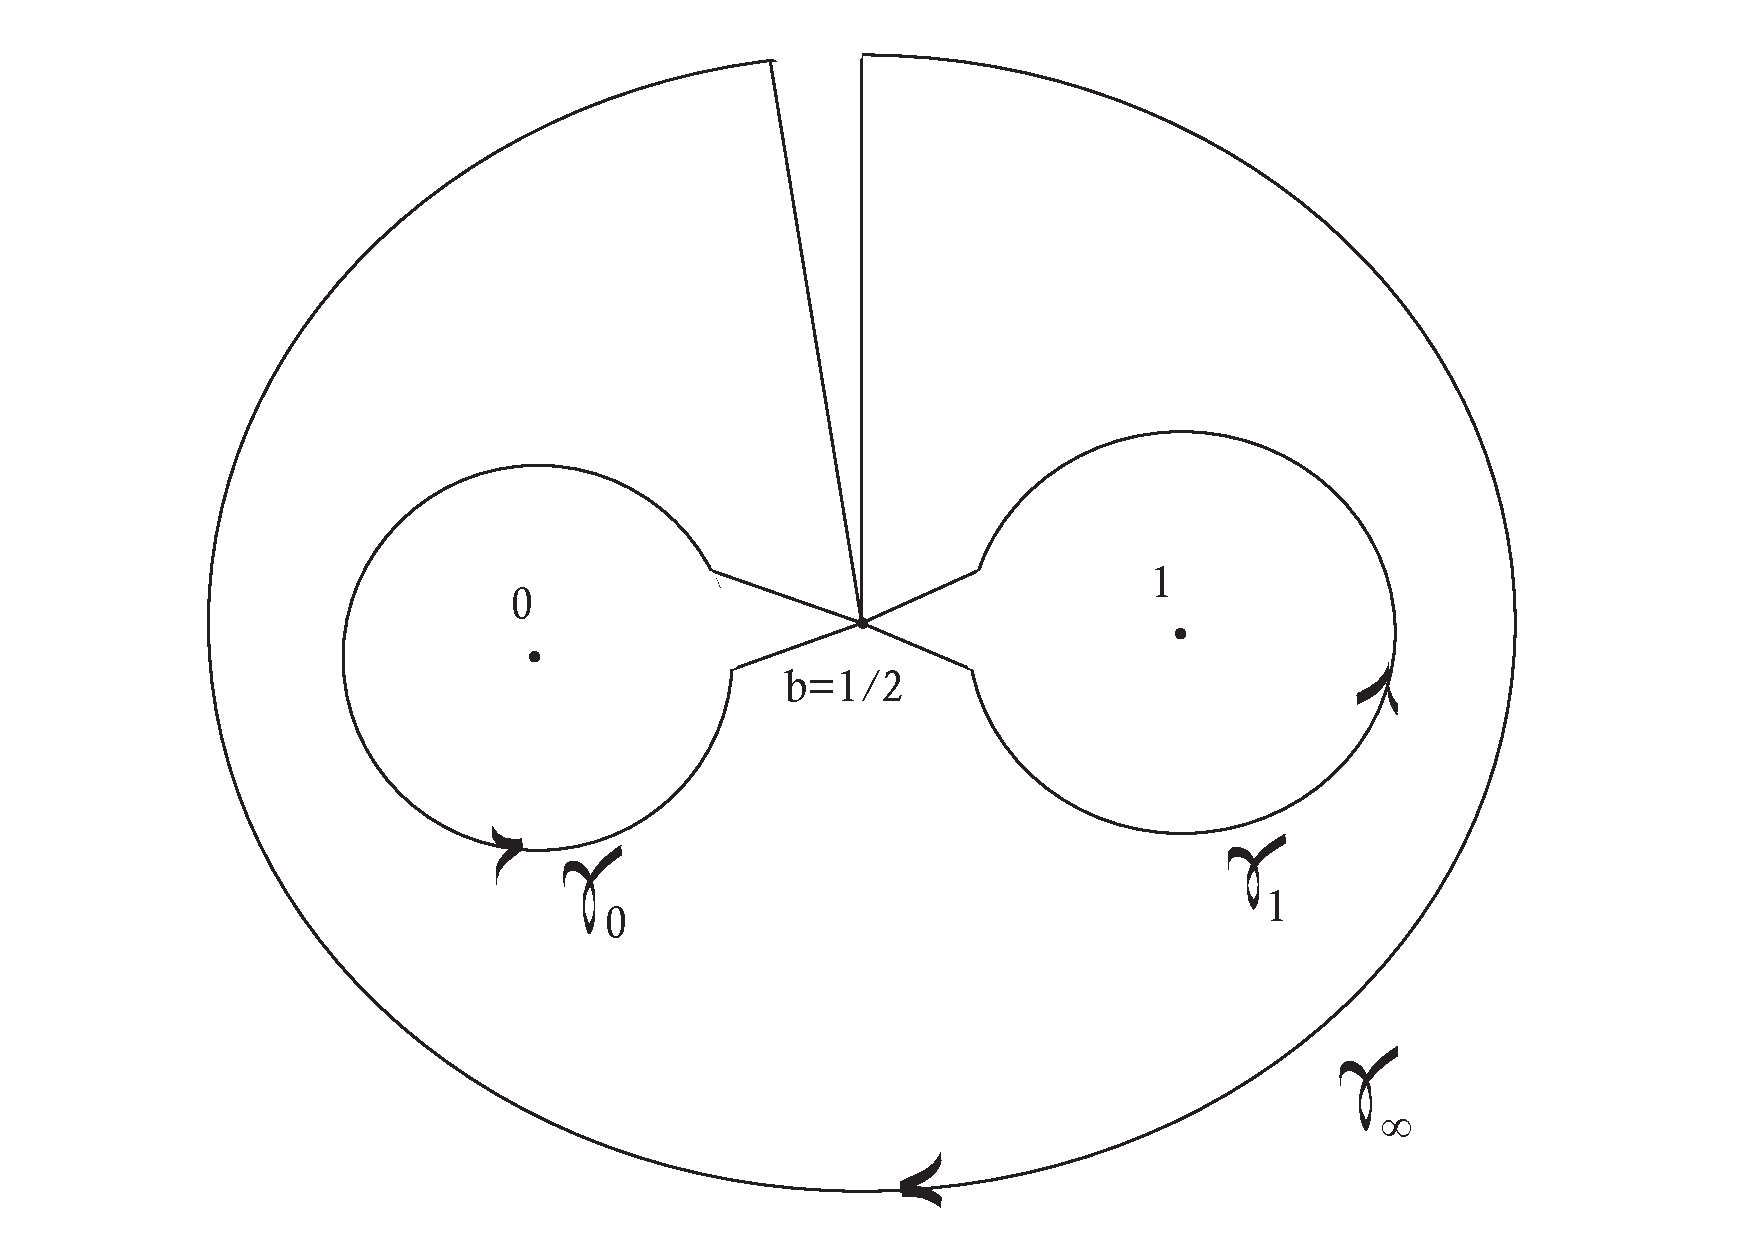
\includegraphics[width=10cm]{lazos3.pdf}
  \caption{Lazos anclados en $b=\frac{1}{2}$} \label{lazos3}
\end{figure}


El problema de hallar la monodrom\'ia respectiva a una ecuaci\'on diferencial es un problema complicado, afortunadamente existen m\'etodos que nos permiten hallar (en ciertos casos) la monodrom\'ia de la ecuaci\'on hipergeom\'etrica y tambi\'en el grupo de monodrom\'ia para soluciones particulares. En los siguientes cap\'itulos hallamos la monodrom\'ia de la ecuaci\'on hipergeom\'etrica y uno de los grupos de monodom\'ia respecto de las soluciones dadas en \ref{sec:sol_ec_hip}.


\section{Monodrom\'ia de la ecuaci\'on hipergeom\'etrica}

En esta secci\'on encontramos la monodrom\'ia de la ecuaci\'on hipergeom\'etrica a traves de su esquema de Riemann por medio de propiedades locales y la relaci\'on de Fuchs, utilizando fuertemente que la ecuaci\'on hipergeom\'etrica resulta ser irreducible.

Sea $G=\pi_{1} (D,b) $ y $\gamma_{j} \in G, (j=0,1,\infty )$, lazos en $b$. Sea $\rho: G \rightarrow GL(2,\mathbb{C}) $ una representaci\'on de monodrom\'ia del esquema de Riemann

\[ \left( \begin{array}{ccc}
0 & 1 & \infty \\
\rho_{1} & \sigma_{1} & \tau_{1} \\
\rho_{2} &\sigma_{2} & \tau_{2}  \end{array} \right)\]


Dado que 
\begin{equation}
\rho (\gamma_{1} \cdot \gamma_{0}) = \rho(\gamma_{\infty})^{-1}
\end{equation}

 ya que 
 \begin{equation}
 \gamma_{\infty}^{-1}=\gamma_{1} \gamma_{0}  y \gamma_{0}\gamma_{1}        
 \end{equation}
 
 
 es conjugado a $\gamma_{1} \gamma_{0}$, tenemos;

\begin{eqnarray} %equation
 \label{eqnarray:ecuacion1} \lbrace \varepsilon (\rho_{1}), \varepsilon (\rho_{2}) \rbrace \ conjunto \ de \ eigenvalores \ de \ \rho (\gamma_{0}) \\
 \lbrace \varepsilon (\sigma_{1}), \varepsilon (\sigma_{2}) \rbrace \  conjunto \ de \ eigenvalores \ de \ \rho (\sigma_{1}) \\
\lbrace \varepsilon(-\tau_{1}), \varepsilon (-\tau_{2}) \rbrace \  conjunto \ de \ eigenvalores \ de \ \rho (\sigma_{0} \sigma_{1})
\end{eqnarray}

Donde $\varepsilon (\cdot) = exp(2 \pi i \cdot)$. La clase de conjugaci\'on de $\rho$, es decir la monodrom\'ia de $RE(\rho,\sigma,\tau)$ esta casi determinada por los eigenvalores, y esta completamente determinada si la monodrom\'ia es irreducible.

\begin{defn}La ecuaci\'on de Riemann $RE(\rho,\sigma,\tau)$ se dice irreducible s\'i la monodrom\'ia es irreducible
\end{defn}

\begin{thm} \label{riemann-irreducible}

La ecuaci\'on de Riemann es irreducible si y solo si

$$\rho_{i} + \sigma_{j} + \tau_{k} \notin \mathbb{Z}, (i,j,k=1,2)  $$
Bajo esta condici\'on la representaci\'on $\rho $ se expresa hasta conjugaci\'on por las siguientes matrices:

$$ \rho (\gamma_{0}) \leftrightarrow  \begin{pmatrix}
 \varepsilon(\rho_{1})& 1\\
 0& \varepsilon(\rho_{2})
 \end{pmatrix}  ,\ \ \
\rho (\gamma_{1}) \leftrightarrow \begin{pmatrix}
 \varepsilon(\sigma_{1})& 0\\
 b& \varepsilon(\sigma_{2})
 \end{pmatrix}
$$

 Y el n\'umero $b$ esta dado por $b= \varepsilon(-\tau_{1}) + \varepsilon(-\tau_{2}) - \varepsilon(\rho_{1} + \sigma_{1}) - \varepsilon(\rho_{2} + \sigma_{2})$, y $\varepsilon(\cdot) =exp(2 \pi i \cdot)$. Todas las representaciones  obtenidas al intercambiar $\rho_{1},\rho_{2}$ y/o $\sigma_{1},\sigma_{2}$ son mutuamente conjugadas.

\end{thm}

En nuestro caso tenemos el esquema de Riemann;

\[ \left( \begin{array}{ccc}
0 & 1 & \infty \\
0 & 0 & a \\
1-c &c-a-b & b  \end{array} \right)\]

Y verificamos si satisface las condiciones del teorema, tenemos los siguientes casos:


\begin{enumerate}
\item 0+0+ a = a
\item 0 + c-a-b + b = c-a
\item 0 + c-a-b + a = c-b
\item 1-c + 0 + a= 1-c +a
\item 1-c + 0 + b=1-c+b
\item 1-c + c-a-b + b = 1-a
\item 0 + 0 + b = b
\item 1-c + c- a- b + a = 1-b
\end{enumerate}


 Queremos calcular $a,c-a,c-b,1-c+a,1-c+b,1-a,b,1-b$, y estamos considerando que los exponentes $ 1-c,c-a-b,a-b$ son imaginarios puros, por lo que basta probar que ninguno de los anteriores estan en $\mathbb{Z}$.

No es dif\'icil verificar que $b = \frac{1-i(\theta_{0} + \theta_{1} +\theta_{2})}{2} \notin \mathbb{R}$. Para $a$ tenemos;

$$a= \frac{1-i(\theta_{0} + \theta_{1} - \theta_{2})}{2}$$

Y podemos ver que $a \notin \mathbb{R}$ o $ a = \frac{1}{2}$  de cualquier modo $a \notin \mathbb{Z}$. Para $c-a$ se tiene;

$$c-a = \frac{1 + i (-\theta_{0} + \theta_{1} - \theta_{2})}{2}$$

Por lo que de nuevo $c-a \notin \mathbb{R}$ o $c-a = \frac{1}{2}$, y de cualquier modo $c-a \notin \mathbb{Z}$. Para $c-b$ se tiene;

$$c-b =\frac{1+i(\theta_{2} + \theta_{1} - \theta_{0})}{2} $$

Entonces $c-b \notin \mathbb{R}$ o $c-b =\frac{1}{2}$ y en cualquier caso $c-b \notin \mathbb{Z}$. Para $1-c+a$ notamos que $1-c+a= - (c-a-1 )$ y $c-a-1 = -\frac{1}{2}$ o $c-a-1 \notin \mathbb{R}$. En los casos restantes un proceso an\'alogo nos enseña que ninguno de los n\'umeros considerados esta en $\mathbb{Z}$.

Invocamos el teorema \ref{riemann-irreducible} al esquema de Riemann que hallamos para nuestra ecuaci\'on, y obtenemos que las matrices que generan la monodromia de la ecuaci\'on hipergeom\'etrica con exponentes imaginarios puros son:

$$ \rho (\gamma_{0}) \leftrightarrow  \begin{pmatrix}
 1& 1\\
 0& e^{2 \pi i (1-c)}
 \end{pmatrix}  ,\ \ \
\rho (\gamma_{1}) \leftrightarrow \begin{pmatrix}
 1& 0\\
 b& e^{2 \pi i (c-a-b)}
 \end{pmatrix}
$$

Con $b = e^{-2 \pi i a} + e^{-2 \pi i b} -1 -e^{2 \pi i (1-a-b)}$, y la monodrom\'ia de la ecuaci\'on hipergeom\'etrica es generada por $\rho (\gamma_{0}), \rho (\gamma_{1})$ en $GL(2, \mathbb{C})$.


\section{Grupo de monodrom\'ia con las soluciones dadas por la serie hipergeom\'etrica}

 En este cap\'itulo pretendemos dar a conocer el grupo de monodrom\'ia con el par de sistemas fundamentales de soluciones hallados en \ref{sec:sol_ec_hip}, utilizando las identidades de $Gauss-Kummer$. El enfoque principal en este cap\'itulo es exponer las herramientas necesarias para ese prop\'osito y los resultados principales que llevan a una expresi\'on del grupo de monodrom\'ia con los sistemas fundamentales de soluciones dadas. Los teoremas y resultados de este cap\'itulo pueden encontrarse en \cite{gausspainleve} as\'i como sus demostraciones, y se remite al lector a dicha bibliograf\'ia para un desarrollo m\'as profundo de lo expresado aqu\'i. \\


 Queremos resolver el problema de conexi\'on utilizando las identidades de $Gauss-Kummer$ y encontrar generadores para el grupo de monodrom\'ia de la ecuaci\'on diferencial hipergeom\'etrica con las soluciones dadas en \ref{sec:sol_ec_hip}. Los sitemas fundamentales de soluciones son $(f_{0}(x;0),f_{0}(x;1-c))$ y $(f_{1}(x;0),f_{1}(x;c-a-b))$ , queremos encontrar una relaci\'on entre estos sistemas.

 \begin{thm} Si ninguno de los exponentes $c$ o $c-a-b$ es un entero entonces

 $$ \label{relacion_sistemas_soluciones} (f_{0}(x;0),f_{0}(x;1-c))=(f_{1}(x;0),f_{1}(x;c-a-b))P$$

 Donde $P$ es la matriz definida por

$$ \label{matriz_conexion} P =  \begin{pmatrix}
 \frac{\Gamma(c) \Gamma (c-a-b)}{\Gamma(c-a) \Gamma(c-b)} & \frac{\Gamma(2-c) \Gamma (c-a-b)}{\Gamma(1-a) \Gamma(1-b)}\\
 \frac{\Gamma(c) \Gamma (c-a-b)}{\Gamma(a) \Gamma(b)} & \frac{\Gamma(2-c) \Gamma (c-a-b)}{\Gamma(a-c+1) \Gamma(b-c+1)}
 \end{pmatrix}
$$

Y $\Gamma$ es la funci\'on Gamma.
 \end{thm}

 En nuestro caso los exponentes $1-c$ y $c-a-b$ estan en $i\mathbb{R}$ por lo que $c$ y $c-a-b$ cumplen las condiciones del teorema. \\

 Los lazos en la fig. \ref{lazos3} nos sirven para hacer la continuaci\'on anal\'itica del sistema fundamental de soluciones $(f_{0}(x;0),f_{0}(x;1-c))$ y gracias al teorema anterior sabemos que tendremos una matriz conjugada bajo $P$ que ser\'a generador de nuestro grupo de monodrom\'ia.

 \begin{thm}
 Sea $\gamma_{v}, (v=0,1) $ lazos con punto inicial y final $b=\frac{1}{2}$ definidos en \ref{lazos3}, supongamos que ni $c$ ni $c-a-b$ son enteros. La continuaci\'on anal\'itica del sistema fundamental de soluciones $\mathfrak{F}=(f_{0}(x;0),f_{0}(x;1-c))$ a lo largo de $\gamma_{v}$ esta dada por

 $$\label{sistema_soluciones_continuacion_analitica} \gamma_{v_{*}} \mathfrak{F} = \mathfrak{F} A_{v} , (v=0,1)$$

 Donde $A_{v} $ son matrices definidas por

 $$ \label{Matrices_teorema_monodromia_grupo}  A_{0} =  \begin{pmatrix}
 1& 0\\
 0& \varepsilon (-c)
 \end{pmatrix}  ,\ \ \
A_{1} = P ^{-1}\begin{pmatrix}
 1& 0\\
 0& \varepsilon (c-a-b)
 \end{pmatrix} P
$$

Donde $P$ esta dada por \ref{matriz_conexion} y $\varepsilon(\cdot) = exp(2 \pi i \cdot )$. El grupo de monodrom\'ia respecto al sistema fundamental de soluciones $\mathfrak{F} $ esta generado por $A_{0}$ y $A_{1}$.
 \end{thm}




% ----------------------------------------------------------------------

	

%: ----------------------- overall methodology ------------------------
% introduction

% this file is called up by thesis.tex
% content in this file will be fed into the main document

%: ----------------------- introduction file header -----------------------
%\begin{savequote}[50mm]
%Historical methodology, as I see it, is a product of common sense applied to circumstances.
%\qauthor{Samuel E. Morison}
%\end{savequote}


\chapter{Grupo de Schottky de la ecuaci\'on hipergeom\'etrica}
\label{cha:grupo schottky}

% the code below specifies where the figures are stored
%\ifpdf
  %  \graphicspath{{3_overall_methodology/figures/PNG/}{3_overall_methodology/figures/PDF/}{3_overall_methodology/figures/}}
%\else
 %   \graphicspath{{3_overall_methodology/figures/EPS/}{3_overall_methodology/figures/}}
%\fi


%-------------------------------------------------------------------------

%\cite{turing1950computing}

Nuevamente consideramos la ecuaci\'on hipergeom\'etrica

  $$x(1-x)\frac{d^{2}u}{dx^{2}} +  \lbrace c- (a+b+1 )x \rbrace \frac{du}{dx} - abu=0 $$

Cuyos exponentes son

$$ 1-c = i\theta_{0}, \ c-a-b = i \theta_{1},  \ a-b=i\theta_{2}  $$

Donde supondremos $\theta_{0}, \theta_{1} , \theta_{2} > 0$. Para cualesquiera dos soluciones linealmente independientes $u_{1}$ y $u_{2}$ tenemos el mapeo multivaluado $$s: \mathbb{C} -\lbrace0,1  \rbrace \ni x \mapsto u_{1}(x):u_{2}(x) \in \mathbb{P} := \mathbb{C} \cup \lbrace \infty \rbrace $$ llamado el mapeo de Schwarz.

\section{Dominios fundamentales}

 En \cite{geometricstudy} se pueden encontrar un  dominio $F_{x} $ en $\mathbb{C}$ y un dominio $F_{s}$ en $\widehat{\mathbb{C}}$ tal que el mapeo

 $$ s|_{F_{x}}: F_{x} \rightarrow F_{s}$$

  Es un biholomorfismo  y el mapeo $s$ se puede recuperar via el mapeo restringido $s|_{f_{x}}$ a traves del principio de reflexi\'on de Schwarz (\cite{geometricstudy}), estos se llaman dominios fundamentales para el mapeo de Schwarz. \\

\begin{figure}[h]
  \centering
  % Requires \usepackage{graphicx}
  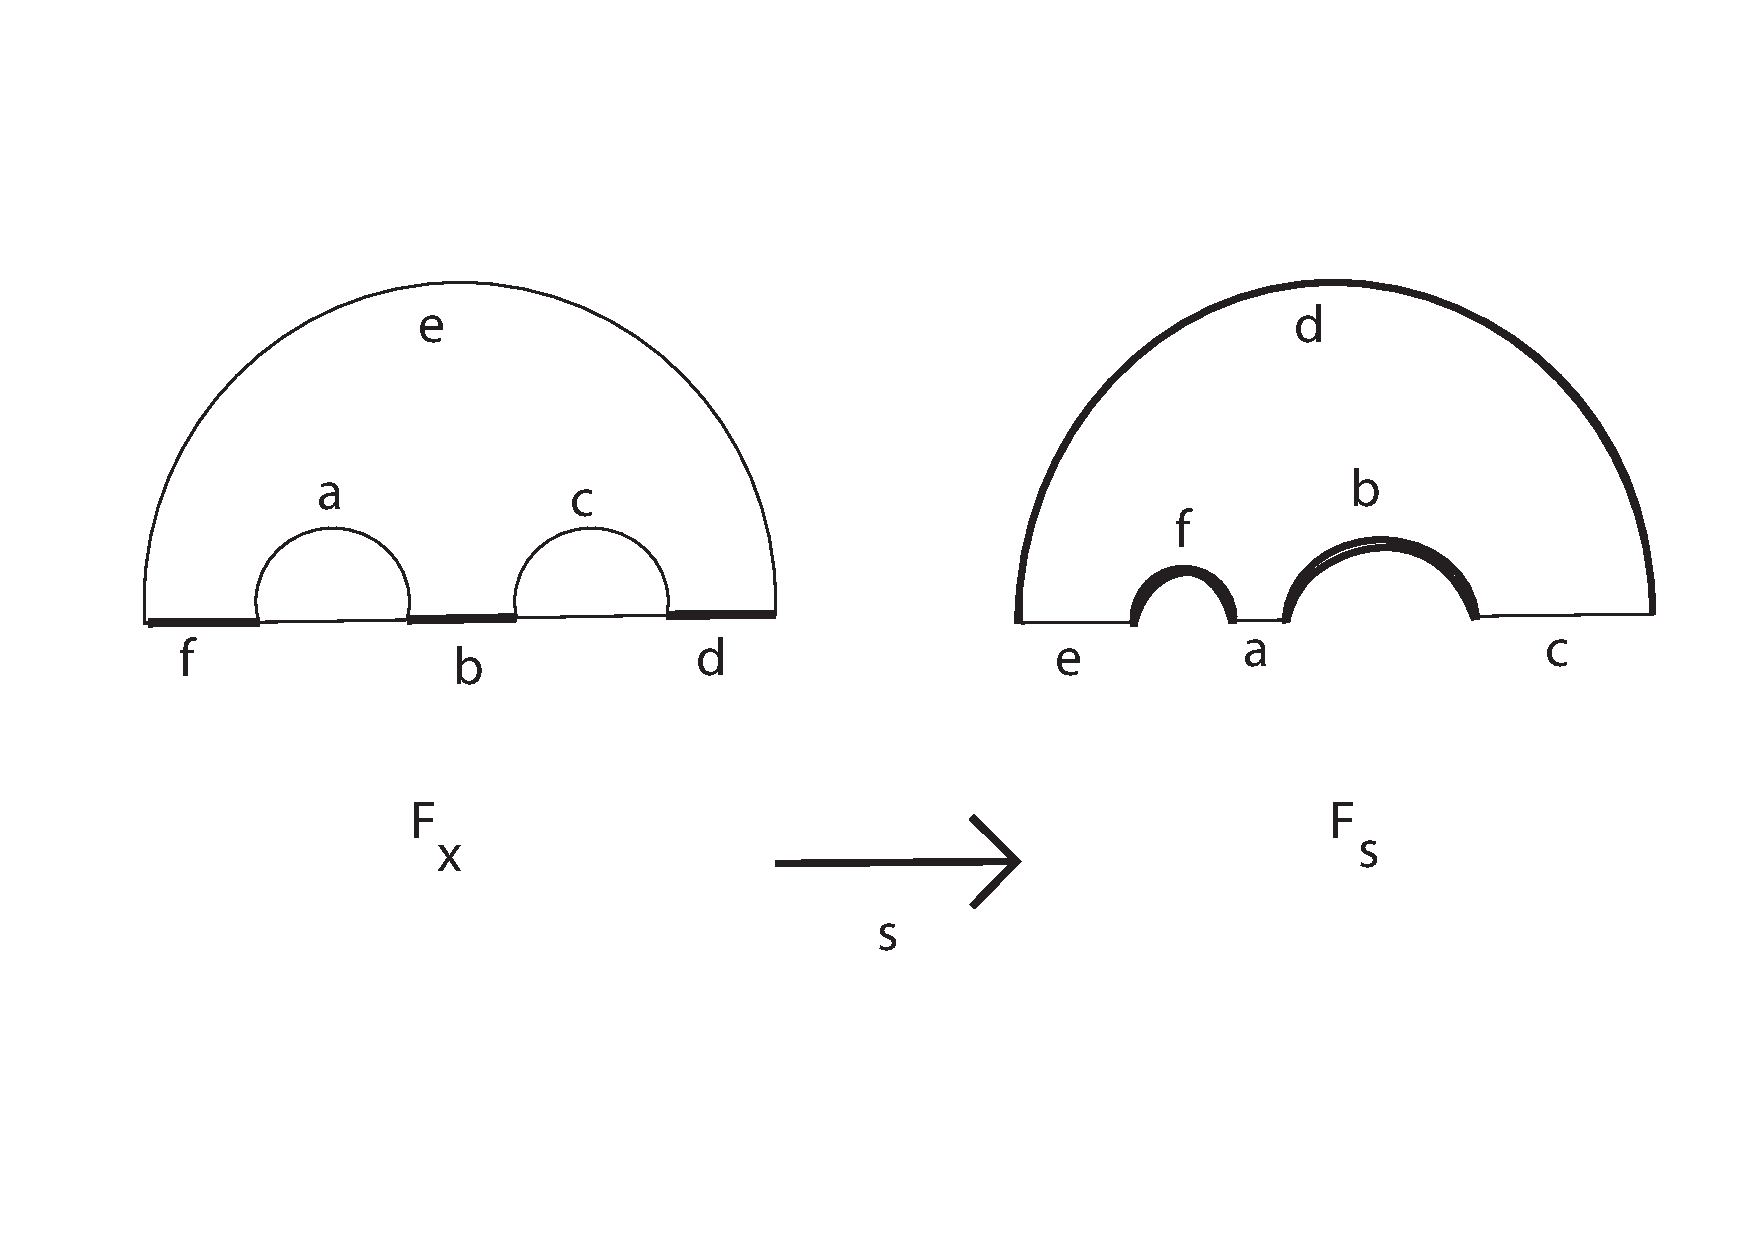
\includegraphics[width=10cm]{dominiosfundamentales.pdf}\\
  \caption{Dominios fundamentales}\label{dominiosfundamentales}
\end{figure}



Denotemos por $C(c,r)$ el c\'irculo en el plano $s$ con centro $c$ y radio $r$ y considerense los tres c\'irculos disjuntos en el plano $s$

$$ C_{1} = C(0,1), C_{2}=C(0,T), C_{3}= C(-C,R)$$

Donde $T=e^{\theta_{1} \pi}, r= e^{-\theta_{0} \pi}$

$$ C=\frac{\xi (1-r^{2})}{\xi^{2}-r^{2}},R=\frac{r(1-\xi^{2})}{\xi^{2}-r^{2}}, \xi =( \frac{cosh \theta_{2} \pi + cosh(\theta_{0}-\theta_{1}) \pi}{cosh \theta_{2} \pi + cosh(\theta_{0} + \theta_{1})\pi} )^{\frac{1}{2}}$$


Cuando $\theta_{2} = 0$

$$ Cosh (\theta_{0}-\theta_{1})\pi = \frac{1+(rt)^{2}}{2rT}$$

y

$$Cosh( \theta_{0} + \theta_{1})\pi = \frac{r^{2} + T^{2}}{2rT}$$

 Y tambi\'en $Cosh\theta_{2}\pi = 1 $ por lo que

 $$\xi^{2}|_{\theta_{2}=0} = \frac{1 + \frac{1 + (rt)^{2}}{2rT}}{ 1 + \frac{r^{2 } + T^{2}}{2rT}} = \frac{\frac{2rT + 1 + (rt)^{2}}{2rT}}{\frac{2rT + r^{2} + T^{2}}{2rT}}= \frac{T^{2} + 2rT +1}{r^{2} + 2rT + T^{2}} = \frac{(rT  + 1)^{2}}{(r + T)^{2}}$$

Entonces $\xi|_{\theta_{2}=0} = \frac{Tr + 1}{ T +r}$

Ya que $T>1$ y $r <1$ tenemos por un lado $r^{2}<1$ entonces $Tr + r^{2} < Tr + 1$, es decir, $r(T+r)< Tr +1$, entonces;$r<\frac{Tr + 1}{T+r}$.

Por otro lado; $r<1$ y tambi\'en $T-1>0$ por lo que $(T-1)r < T-1$ entonces $Tr-r < T-1$ y luego $Tr +1 < T+r$ por lo que $\frac{Tr +1}{T +r} < 1$
Dado que $\xi $ como una funci\'on de $\theta_{2} \geq 0$ incrementa de manera mon\'otona a 1 y $$1 > \xi |_{\theta_{2} =0} = \frac{Tr+1}{T+r} > r $$

tenemos

$$C-R-1 =\frac{\xi(1-r^{2})}{\xi^{2}-r^{2}} - \frac{r(1-\xi^{2})}{\xi^{2}-r^{2}}-1= \frac{\xi-\xi r^{2} -r + r\xi^{2}-\xi^{2} - r^{2}}{\xi^{2} - r^{2}}$$
$$= \frac{\xi-r + \xi r(-r + \xi)-(\xi -r)(\xi + r)}{ \xi^{2} - r^`{2}}$$
$$= \frac{(\xi -r)(1 + \xi r - (\xi +r))}{(\xi +r)(\xi -r)}$$
$$=\frac{1 + \xi r -(\xi +r)}{\xi +r}=\frac{(1-r)(1-\xi)}{\xi +r} > 0  $$

$$T-C-R =\frac{(T+r)\xi - (Tr +1)}{\xi -r} >0$$

y tenemos

$$-T < -C -R < -C + R < -1< 1< T $$

\begin{rem}
Existe una relaci\'on entre el n\'umero $\xi $ y los elementos de la matriz $P $ en el teorema \ref{matriz_conexion} y una relaci\'on entre dichos elementos, estas relaciones son importantes para verificar m\'as adelante que en efecto podemos decir que el grupo de monodrom\'ia de la ecuaci\'on hipergeom\'etrica es un grupo de $Schottky$, Las relaciones son las siguientes;

$$  \  P = \begin{pmatrix}
      D & C \\
      B & A
        \end{pmatrix} , \ \ \xi = \frac{|A|}{|B|}$$

 Y tambi\'en $A=\bar{D}, \ B= \bar{C}$
\end{rem}


El dominio en el semi-plano superior, acotado por $C_{1}, C_{2}, C_{3}$ y el eje real, puede servir como un dominio fundamental $F_{s}$, y tiene la forma de un puente de doble arco como en la figura \ref{dominiosfundamentales}. El dominio fundamental $F_{x}$ tambi\'en tiene la forma de de un  puente de doble arco como en la figura \ref{dominiosfundamentales}, y esta acotado por tres segmentos reales y tres curvas que no son parte de circunferencias.

\section{El grupo de monodrom\'ia generado por reflexiones}

Gracias a estos dominios fundamentales y el principio de reflexi\'on de Schwarz (\ref{cha:apendice}) aplicado a lo largo de los lados, el grupo de monodrom\'ia de la ecuacion diferencial se puede describir como sigue. La reflexi\'on con respecto al c\'irculo $C(c,r)$ donde $c$ es real, esta dada por  $$\psi(c,r): s \mapsto \frac{r^{2}}{\bar{s} - c}  $$

Sea $\bar{\Lambda}$ el grupo generado por las tres reflexiones respecto a los c\'irculos $C_{1},C_{2},C_{3}$, respectivamente. El grupo de monodrom\'ia $\Lambda_{\theta}$ de la ecuaci\'on hpergeom\'etrica es el subgrupo de $\bar{\Lambda}$, de \'indice 2 que consiste de las palabras pares de $\psi_{1},\psi_{2}, \psi_{3}$.

Por otro lado, para el c\'irculo $C(c,r)$ definimos la transformaci\'on fraccional lineal de orden 2 que fija los dos puntos de intersecci\'on del c\'irculo y el eje real: $$\gamma (c,r): s \mapsto \frac{r^{2}}{s-c} + c $$


Sea $\Gamma _{\theta},$ el grupo generado por tres involuciones $\gamma_{1},\gamma_{2},\gamma_{3}$ con respecto a los c\'irculos $C_{1},C_{2},C_{3}$, respectivamente.
El grupo de monodrom\'ia $\Lambda_{\theta }$ es el subgrupo de $\Gamma_{\theta}$, de \'indice 2 que consiste de las palabras pares de $\gamma_{1},\gamma_{2},\gamma_{3}$. Sea $\omega ( \subset \mathbb{P}^{1})$ el dominio de discontinuidad de $\Gamma_{\theta}$ y el grupo de Schotky $\Lambda_{\theta}$.

Esta representaci\'on tiene algunos problemas, aunque la ecuaci\'on hipergeom\'etrica es sim\'etrica respecto de $\theta_{0},\theta_{1},\theta_{2}$, los tres c\'irculos $C_{1},C_{2},C_{3}$ no lo son. Por ejemplo si $\theta_{2} \rightarrow 0$ los c\'irculos $C_{2}$ y $C_{3}$ se tocan, y si $\theta_{1} \rightarrow 0$ entonces $C_{3}$ tiende a un punto y $C_{1}$ y $C_{2}$ coinciden, m\'as a\'un ya que $C_{1}$  y $C_{2}$ son concentricos. Hacemos un cambio de coordenadas como sigue :

$$s \mapsto \frac{(3 + T^{2})s + 1 + 3T^{2}}{4(s + T^{2})} $$

 entonces los diametros de los c\'irculos en el eje real estan dados por

  $$ C_{1}:[s_{4},s_{5}],C_{2}:[s_{1},s_{6}],C_{3}:[s_{2},s_{3}]$$

\begin{figure}[h]
  \centering
  % Requires \usepackage{graphicx}
  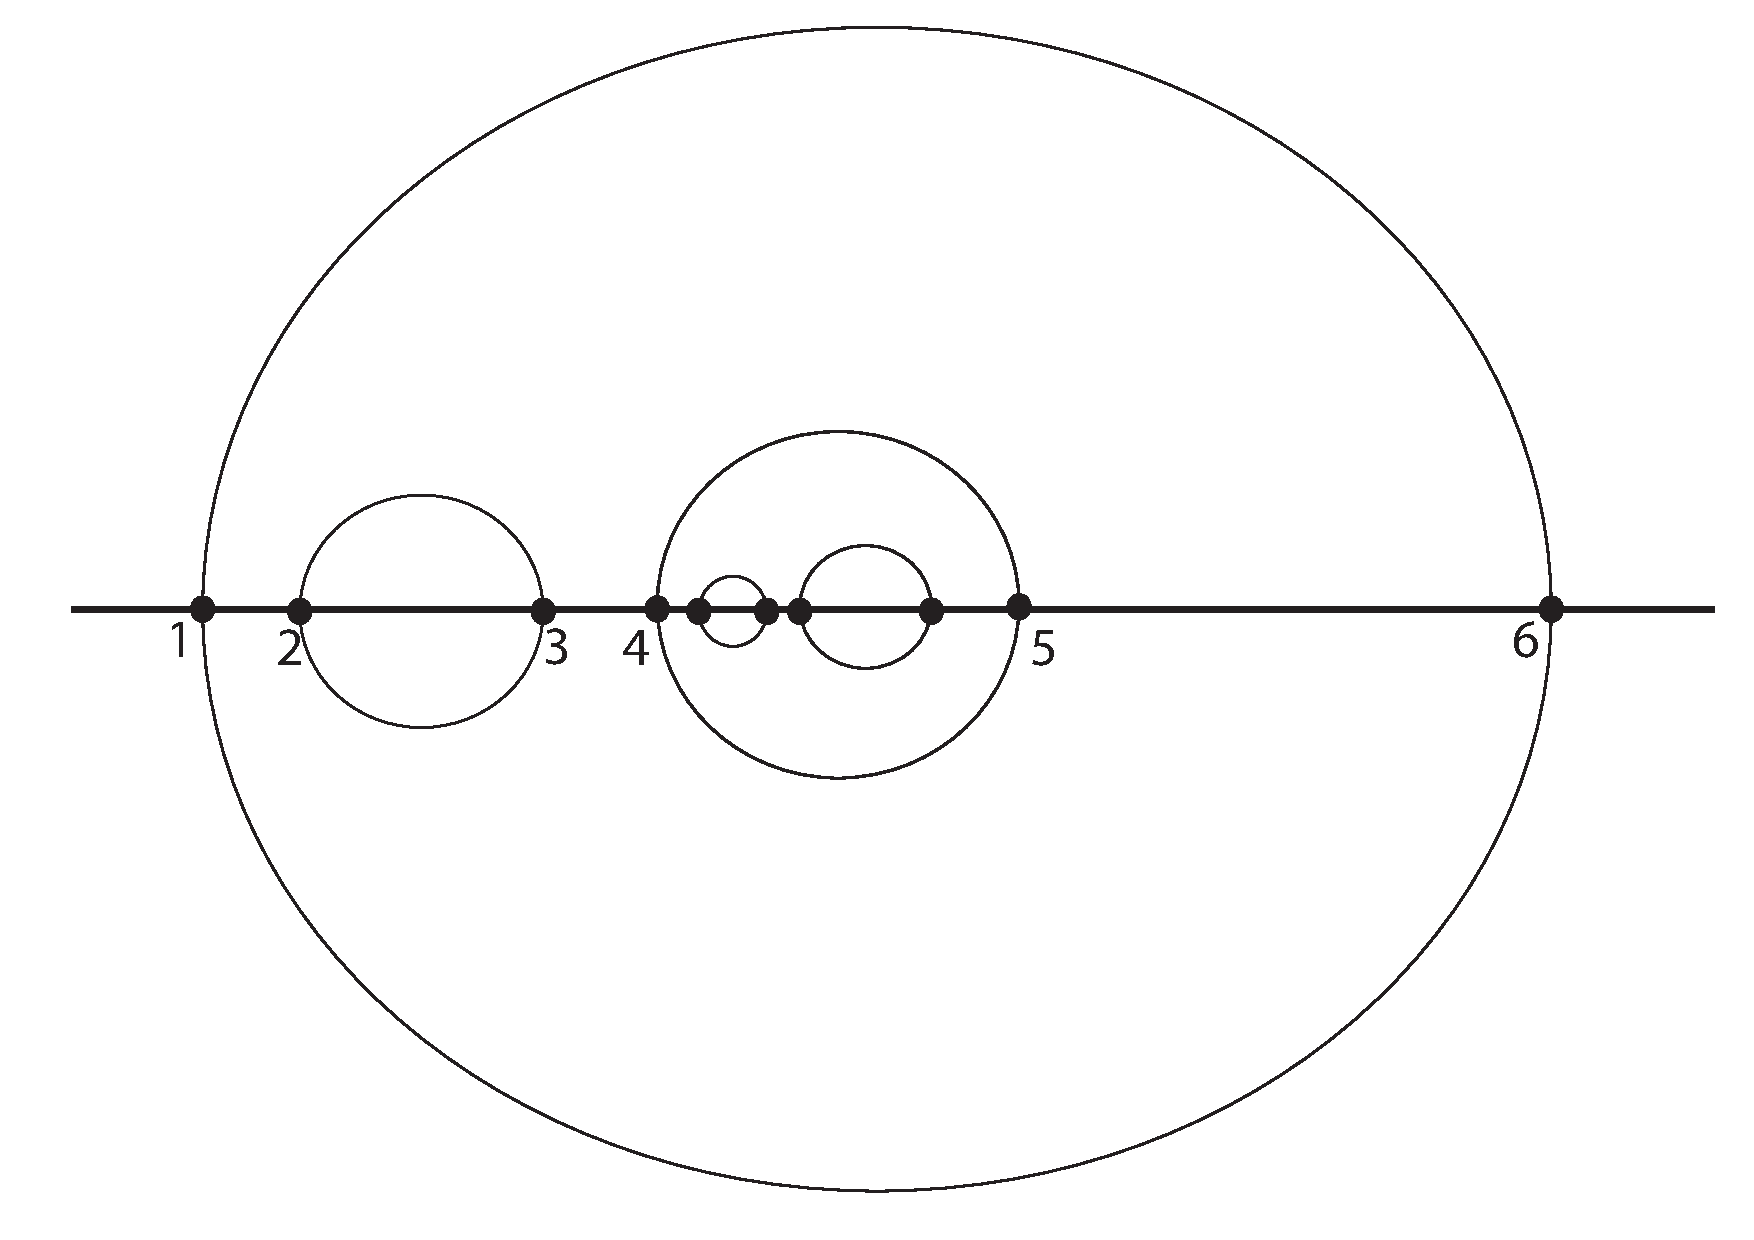
\includegraphics[width=10cm]{nuevosdiametros.pdf}\\
  \caption{C\'irculos $C_{1},C_{2},C_{3}$}\label{nuevosdiametros}
\end{figure}


Donde $$s_{1} = - \frac{(1-T)^{2}}{4T} , s_{2}= - \frac{(T-1)^{3} - (3 + T^{2})(T-C-R)}{4(T^{2} - T + T -C-R)}$$



$$s_{3}= -\frac{(1+T^{2})(C-R-1)}{4(T^{2}-1-(C-R-1))} + \frac{1}{2}, s_{4} = \frac{1}{2} $$

$$s_{5} = 1 , s_{6} = \frac{(1+ T)^{2}}{4T} $$


Notemos que $s_{1}< s_{2}< \cdots < s_{6}$, Ahora podemos probar lo siguiente,

\begin{prop} Si $\theta_{1} = 0$ entonces $C_{1}$  y $C_{2}$ se tocan en un punto. Si $\theta_{2} = 0 $ entonces $C_{2}$ y $C_{3}$ se tocan en un punto. Si $\theta_{0} = 0$, entonces $C_{3}$ y $C_{1}$ se tocan en un punto
\end{prop}

\textit{Prueba.}

Cuando $\theta_{1} = 0$, notemos que en este caso $T = e^{\theta_{1} \pi}$ y dado que $\theta_{1} = 0$ se tiene que $T =1$, tambi\'en recordemos que $C_{1}:[s_{4},s_{5}]$ y $C_{2}: [s_{1}, s_{6}]$ y dado que $s_{5} = 1 $ y $s_{6} = \frac{(1+ T^{2})^{2}}{4T} = \frac{(1 + 1^{2})^{2}}{4} = \frac{4}{4} = 1$ concluimos que $C_{1}$ y $C_{2}$ se tocan en $1$.

Si $\theta_{2} = 0$,primero veremos que $T-C-R = 0$, como $\theta_{2}=0$ entonces $\xi = \frac{Tr +1}{ T + r}$ esto implica que $(T+r) \xi = Tr +1$ y como $T-C-R = \frac{(T+r)\xi - (Tr+1)}{ \xi -r} = \frac{Tr+1 - ( Tr+1)}{\xi - r} =0$, Ahora bien $s_{1} = -\frac{1-T^{2}}{4T}$ y $s_{2} = -\frac{(T-1)^{3} - (3 + T^{2})(T-C-R)}{ 4(T^{2} - T + T-C-R)} =- \frac{(T-1)^{3}}{4(T^{2} - T)} =- \frac{(T-1)^{2} (T-1)}{4T (T-1)} = -\frac{(T-1)^{2}}{4T}= s_{1} $ por lo que $C_{2}$ y $C_{3}$ se tocan en $s_{1}$.

Por \'ultimo si $\theta_{0} = 0$ tenemos $r=e^{-\theta_{0} \pi }$ en este caso $r = 1$ mostremos que $C-R-1=0$.De las deducciones anteriores $C-R-1 = \frac{(1-r)(1- \xi)}{ \xi + r}$,Entonces $C-R-1= 0$ ya que $r = 1$, entonces $ s_{3} = \frac{(1+T^{2})(C-R-1)}{ 4(T^{2} -1 -C-R-1)} + \frac{1}{2} = \frac{1}{2}$ ya que $C-R-1 = 0$ y dado que $C_{3}:[s_{2},s_{3}]$ y  $ C_{1}:[s_{4},s_{5}]$ por los calculos anteriores obtuvimos $s_{4}= s_{3}$ (recordando que $s_{4} = \frac{1}{2}$), Concluyendo con la prueba. $\square $



\section{ El grupo de Schottky asociado al grupo de Monodrom\'ia}

Si ahora tomamos como antes las reflexiones $\psi_{1},\psi_{2},\psi_{3}$, definimos las siguientes transformaciones;

$$\gamma_{1}=\psi_{2} \psi_{1} \ , \ \gamma_{2} = \psi_{1} \psi_{3} $$

Y tomamos los c\'irculos $C_{1}, C_{3}$ y $C_{1}' = \psi_{2} (C_{1}), C_{3}'= \psi_{1} (C_{3})$, luego por definici\'on tenemos;

$$\gamma_{1} ( C_{1})= C_{1}'  \ \ , \ \ \gamma_{2} (C_{3}) = C_{3}'$$

Adem\'as tenemos que el exterior de $C_{1}$ se mapea al interior de $C_{1}'$ y el exterior de $C_{3}$ se mapea al interior de  $C_{3}'$, por la definici\'on tenemos un grupo de $Schottky$ de genus 2 (genero 2). Para el grupo de $Schottky$ anterior tenemos que sus transformaciones estan dadas tambi\'en por;

$$\gamma_{1}= sT^{2} \leftrightarrow   \begin{pmatrix}
 1& 0\\
 0& \frac{1}{T^{2}}
 \end{pmatrix} \  ,  \ \gamma_{2} = \frac{s + C}{ -Cs + R^{2} - C^{2}}  \leftrightarrow  \begin{pmatrix}
 1& C\\
 -C&  R^{2} - C^{2}
 \end{pmatrix}   $$

Y notando que $C=\frac{|A||B|(1-r^{2})}{|A|^{2}-|B|^{2}r^{2}}$ y $R^{2} - C^{2} =\frac{|A|^{2}r^{2}-|B|^{2}}{|A|^{2}-|B|^{2}r^{2}} $ podemos ver  que son conjugadas bajo $P$ a las matrices del grupo de monodrom\'ia de la ecuaci\'on hipergeom\'etrica \ref{Matrices_teorema_monodromia_grupo}.
% ----------------------------------------------------------------------






	
%: ----------------------- experiments and results ------------------------
% introduction

% this file is called up by thesis.tex
% content in this file will be fed into the main document

%: ----------------------- introduction file header -----------------------
%\begin{savequote}[50mm]
%The logic of validation allows us to move between the two limits of dogmatism and skepticism.
%\qauthor{Paul Ricoeur}
%\end{savequote}


\chapter{El teorema de Nielsen}
\label{cha:El teorema de Nielsen}

% the code below specifies where the figures are stored
%\ifpdf
%    \graphicspath{{4_experiments_and_results/figures/PNG/}{4_experiments_and_results/figures/PDF/}{4_experiments_and_results/figures/}}
%\else
%    \graphicspath{{4_experiments_and_results/figures/EPS/}{4_experiments_and_results/figures/}}
%\fi


%-------------------------------------------------------------------------

%\cite{turing1950computing}

En este cap\'itulo proponemos un teorema sobre la acci\'on discontinua de  grupos de transformaciones que pretendemos aplicar al caso del grupo de monodrom\'ia de la ecuaci\'on hipergeom\'etrica.

Todo en  este cap\'itulo es pensado en el sentido de Poincar\'e y hacemos un breve recordatorio de los conceptos que ocupamos durante el mismo.

Tratamos de dar una caracterizaci\'on de los grupos propiamente discontinuos de transformaciones lineales fraccionales con c\'irculo principal en el sentido de la teor\'ia de automorfismos.
Representamos al plano hiperb\'olico como una regi\'on circular en el plano complejo, este modelo llamado el disco de poincar\'e se divide en dos partes de $\lbrace z | |z| \leq 1 \rbrace$,el interior
le denominamos $D =\lbrace z | |z| <1 \rbrace$ y la frontera la denominamos  $E =\lbrace z| |z| =1  \rbrace$.  Todas las cosecuencias geom\'etricas las entendemos en el sentido no-euclidio. Tambi\'en denotamos por $\mathbb{H} ^{+}$ al modelo hiperb\'olico del semiplano.\\



Llamamos puntos finales a los extremos de una recta situados en
el c\'irculo infinito, e identificamos tres tipos de relaciones entre las rectas, a saber;
concurrentes, paralelas y divergentes. \\

\begin{defn}
Las rectas Paralelas son dos rectas que tienen un punto
final en com\'un.\\
Las rectas Concurrentes son las que se intersectan en $D$.
\\
Las rectas Divergentes son las que no se intersectan en
nig\'un lugar. \\
\end{defn}



\begin{figure}[h]
  \centering
  % Requires \usepackage{graphicx}
  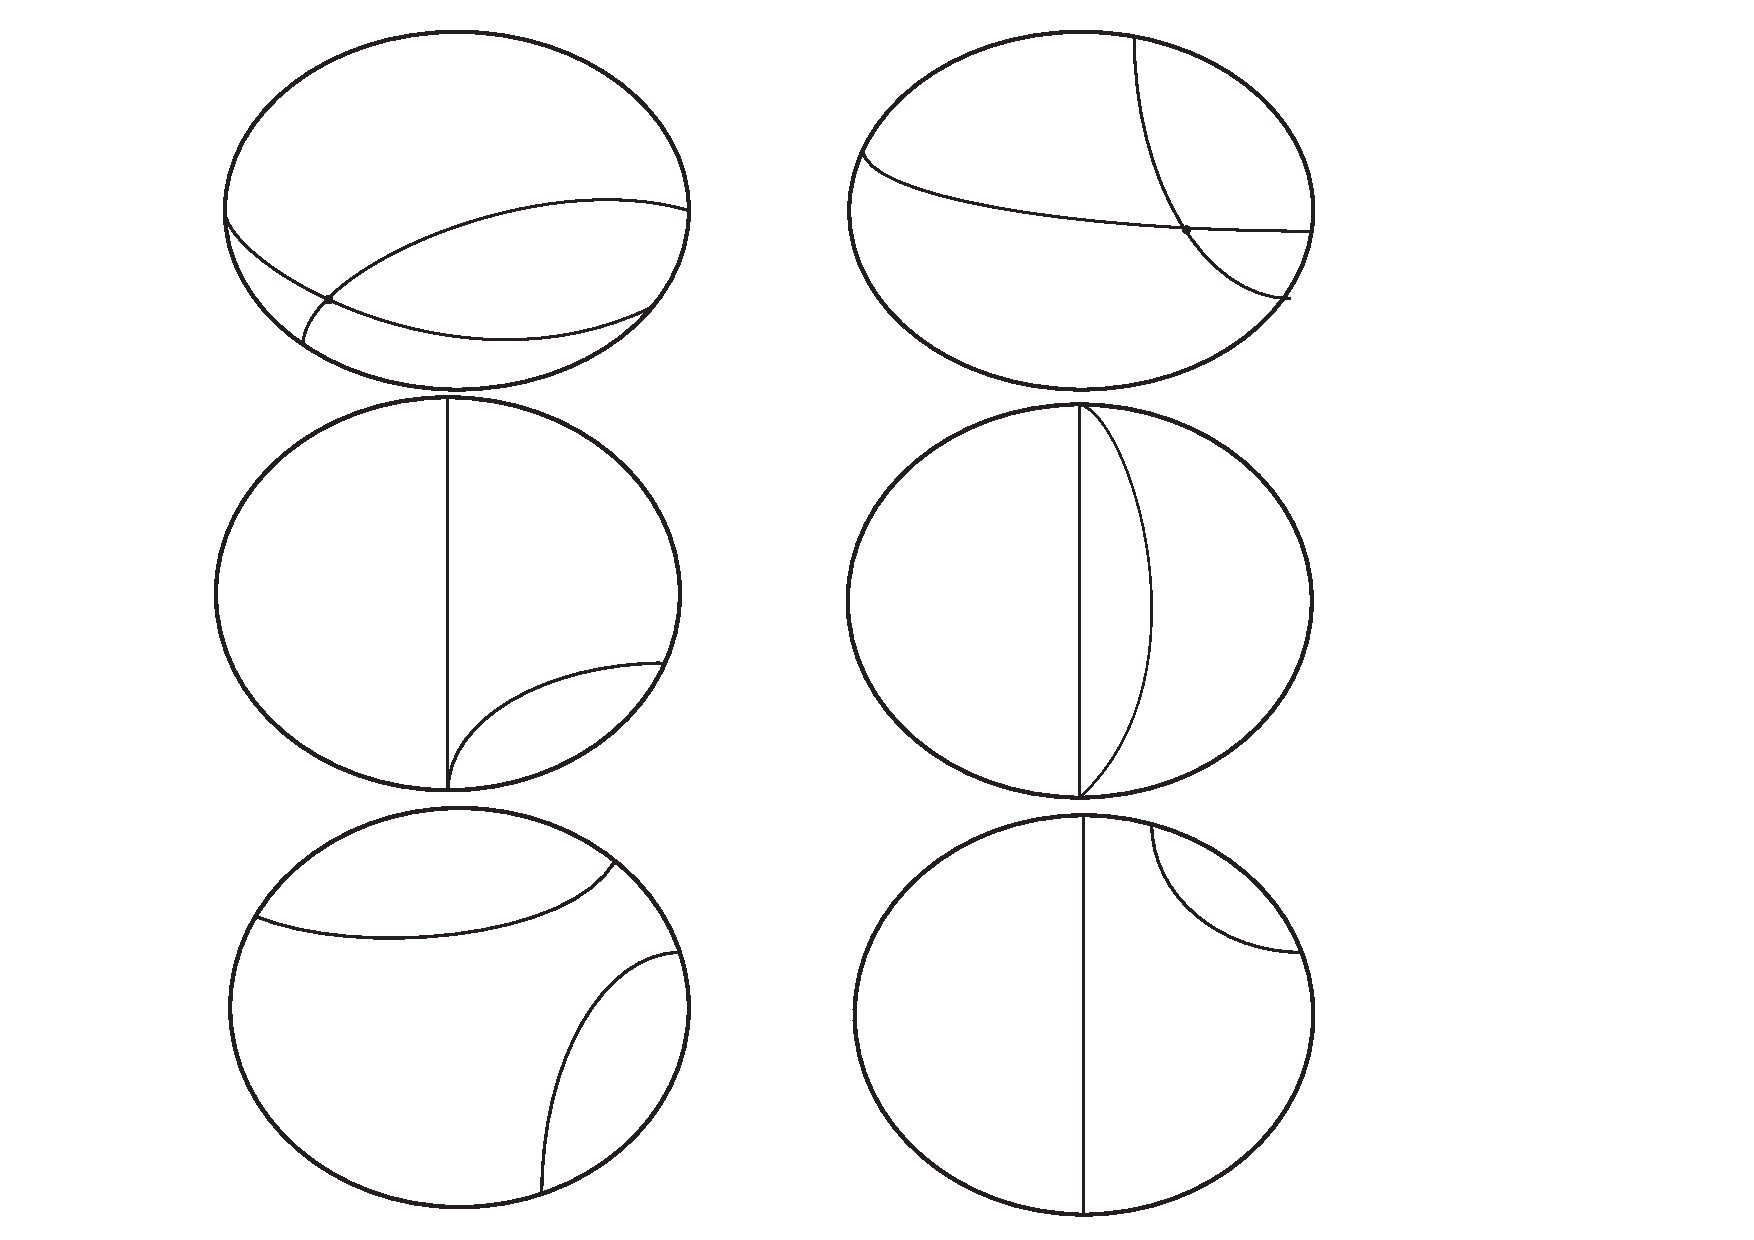
\includegraphics[width=10cm]{rectas-concurrentes-paralelas-divergentes.pdf}\\
  \caption{Rectas hiperb\'olicas concurrentes, paralelas y divergentes respectivamente.}%\label{}
\end{figure}


Los \textbf{Horociclos} son c\'irculos tangentes a alg\'un punto en la
frontera $E$ de $S^{1}$.Es importante dejar en claro que los Horociclos no son geod\'esicas. \\


Los \textbf{hiperciclos} se forman por una recta $\emph{L}$ y un
punto $\textbf{P}$ fuera de ella, el hiperciclo es  el lugar geom\'etrico
de todos los puntos a distancia $d_{H}(\textbf{P},\emph{L})$,  de
$\emph{L}$ y del mismo lado de $P$.  $d_{H}$ es la distancia hiperb\'olica.
 De igual manera los hiperciclos no son geod\'esicas. \\


Dividiremos las transformaciones isom\'etricas en dos grupos, las
que preservan la orientaci\'on y las que no. En el grupo de las que
preservan la orientaci\'ion distinguimos tres tipos distintos de
transformaciones; \\

\begin{defn}
Las transformaciones \textbf{parab\'olicas} tienen un punto fijo en
$E$ y dado un horociclo $K$ tangente en dicho punto fijo a $E$, esta
transformaci\'on tiene un desplazamiento fijo en $K$.


Las tranformaciones \textbf{el\'ipticas} tienen un punto fijo en $D$
y un \'angulo fijo $\phi$ de rotaci\'on en torno al punto fijo.


Las transformaciones \textbf{hiperb\'olicas} tienen dos puntos fijos
en $E$ y una recta invariante, la recta que pasa por dichos puntos
fijos la llamamos eje de la transformaci\'on.


\begin{figure}[h]
  \centering
  % Requires \usepackage{graphicx}
  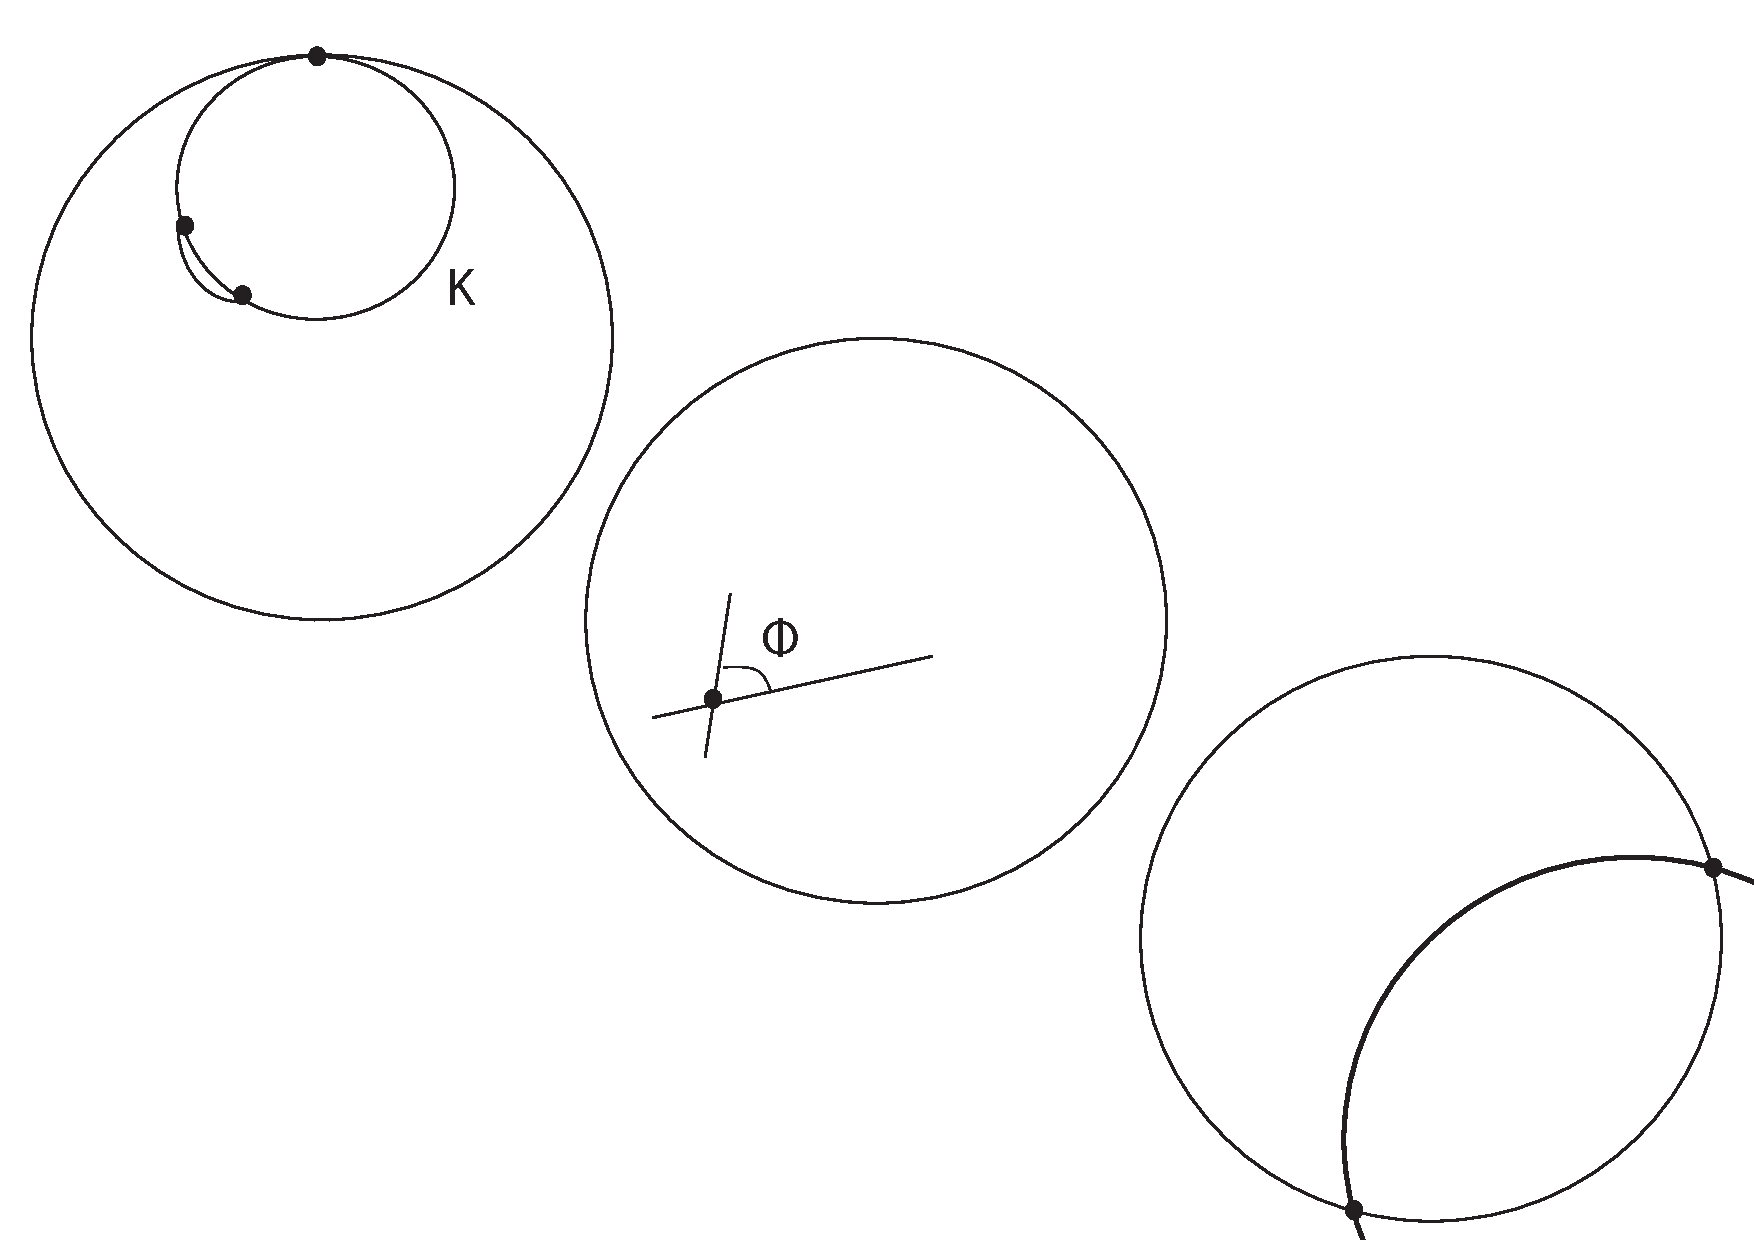
\includegraphics[width=8cm]{definicion40.pdf}\\
  \caption{Representaci\'on de los puntos importantes en las transformaciones hperb\'olicas}\label{definicion40}
\end{figure}


\end{defn}

Si $G$ es un grupo de transformaciones isom\'etricas, un punto
invariante para $G$ es un punto fijo bajo todos los elementos de $G$, de
una manera similar pensamos en una recta invariante. \\

Un par de conjuntos de puntos $M$ y $M'$ en $D + E$ son equivalentes respecto a
$G$ si existe $f \in G$ tal que $M = fM'$. El total de conjuntos
equivalentes de $M$ se denota como la familia $GM$ llamada clase de
equivalencia de $M$, en esta familia si $f_{1},f_{2} \in G  $ y
$f_{1} \neq f_{2 }$ entonces $f_{1}M \neq f_{2}M$ sin importar que
como conjunto sean iguales. \\

\begin{defn}
Decimos que $G$ es discontinuo en un punto $x \in D$,si $x$ no es un
punto de acumulaci\'on de la clase $Gx$, si esto sucede $Gx$ no
tiene puntos de acumulaci\'on en $D$
\end{defn}

\begin{prop}
Si $G$ es discontinuo en $x$, $G$ no tiene puntos de acumulaci\'on en $D$.
\end{prop}

\textit{Prueba}:

Supongamos que $G$ es discontinuo en $x$, existe $m$ tal que $\forall \ i,j, \  d_{H}(g_{i}x,g_{j}x) > m$, de otro modo $x$ ser\'ia un punto de acumulaci\'on de $Gx$. Sea $y$ un punto arbitrario de $D$ y sea $U_{r}$ una vecindad de $y$ de radio $r < m$, entonces a lo m\'as hay un punto $gx$ de $Gx$ en $U_{r}$, si tomamos $V_{r'}$ vecindad de $y$ con $r' < d_{H}(gx,y)$, esa vecindad no contiene puntos de $Gx$. $_{\square}$

Esto implica que si $G$  es discontinuo en un punto de  $D$ entonces es discontinuo en todo
$D$.\\

Las \'unicas isometr\'ias de $\mathbb{H}^{+} $ que preservan la orientaci\'on
son las de $PSL(2,\mathbb{R})$, las transformaciones mencionadas con
anterioridad se encuentran en este grupo. Si $f \in PSL(2,\mathbb{R})$ y $g$  otra transformaci\'on  entonces $gfg^{-1}$ es de la misma clase que $f$.\\

Llamaremos \textbf{reversiones} a las transformaciones que invierten
la orientaci\'on, las reversiones son las \textbf{reflexiones}
respecto a una recta, y las reflexiones compuestas con elementos
hiperb\'olicos a las que llamamos \textbf{h-reflexiones}. \\


La reflexi\'on respecto a una recta hiperb\'olica es la reflexi\'on
respecto a una circunferencia euclidiana. \\


\begin{thm} \label{Teorema-nielsen} [Teorema de Nielsen]
Una condici\'on necesaria y suficiente para que un grupo de
transformaciones isom\'etricas en el plano hiperb\'olico sin puntos
ni lineas invariantes sea discontinuo en $D $ es que los puntos
fijos de los elementos el\'ipticos del grupo, si los hay, no se
acumulen en $D$

\end{thm}

La condici\'on de que no tenga puntos ni rectas invariantes es
necesaria, como podemos ver en los siguientes casos.

\begin{enumerate}
\item Si $G$ es un grupo de elementos parab\'olicos con un mismo punto
fijo al infinito.
\item Si $G$ es un grupo de elementos hiperb\'olicos con una recta fija
dada.
\end{enumerate}

Ninguno de los anteriores contiene elementos el\'ipticos sin embargo
ninguno es discontinuo en $D$.\\

Si $G$ contiene reversiones  y $H$ es un subgrupo de $G$ y adem\'as $H
\subseteq PSL(2,\mathbb{R})$ se tiene que $H$  es normal y de \'indice 2. Es normal ya que si $f \in H$
para cualquier elemento $g \in G$ se tiene que $gfg^{-1}$ es del
mismo tipo que $f$ por lo que $gfg^{1} \in H$, es de \'indice 2,
para ver esto basta probar que si $f,g \in G - H$ entonces $f \cong
g$ equivalentemente que $fg^{-1} \in H$, dado que $f , g$ revierten
orientaci\'on  se tiene que $fg^{-1}$ conserva la orientaci\'on y
por lo tanto esta en
$H$. \\

Una clase de equivalencia $Gx$ es la suma de las clases $Hx$ y $Hgx$
con $g$ una reversi\'on en $G$ ($H \cup Hg = G \Rightarrow Hx \cup
Hgx = Gx $ ), por lo que se concluye que $G$ y $H$
son ambos discontinuos en $D$ o ambos no lo son. En otras palabras $H$ es discontinuo en $D$ si y solo si $G$ lo es.


\begin{prop} Si $G$ no tiene rectas ni puntos invariantes tampoco los
tiene $H$.
\end{prop}

\textit{Prueba}:

 Supongamos que $H$ deja invariantes un punto en $D +E$,
pero ning\'un otro punto (y por tanto ninguna recta), como $G$ no
deja puntos invariantes, existe $g \in G $ tal que $gc \neq c$ luego
el subgrupo $gHg^{-1}$ deja invariante $gc$ pero ningun otro punto en
$D+E$ pero como $H \vartriangleleft G$ se tiene que  $gHg^{-1}=H$ y
como $gc \neq c $ implica que $H$ fija $c$ y $gc$ lo cual es una
contradicci\'on, concluimos que $H$ no deja puntos invariantes. Un
razonamiento an\'alogo nos enseña que $H$ no deja rectas invariantes. $_{\square}$ \\


Desde ahora  $G$ denotar\'a un subgrupo de $PSL(2,\mathbb{R})$ sin
puntos ni rectas invariantes. \\

Ahora probamos el \textbf{Teorema} \ref{Teorema-nielsen} para el caso cuando el grupo tiene elementos el\'ipticos.

\textit{Prueba}:

Primero probaremos que si los puntos fijos de los elementos el\'ipticos se
acumulan $\Rightarrow$ $G$ no es discontinuo en $D$ \\

Supongamos que los puntos fijos de los elementos el\'ipticos se
acumulan en $D$ (tiene un punto de acumulaci\'on en $D$), es posible
encontrar una sucesi\'on de puntos fijos que convergen al punto de
acumulaci\'on digamos $x$ (por ser espacio m\'etrico) y sean estos $y_{1},y_{2},...$ y
$f_{1},f_{2},...$ los respectivos elementos el\'ipticos. Por un lado
$d_{H}(y_{i},x) \leq \epsilon $ para $i$ adecuada, considerando $\lbrace
f_{i}x\rbrace$ podemos notar que

$$ d_{H}(f_{i}x,x) \leq d_{H}(f_{i}x,y_{i}) + d_{H}(y_{i},x) = 2d_{H}(y_{i},x)$$

Lo anterior debido a que $f_{i}$ fija $y_{i}$ y que es una
isometr\'ia. Luego entonces $f_{i}x \rightarrow x$, es decir $Gx$ se
acumula en $x$  por tanto $G$ no es discontinuo en $x$ y por lo
tanto no lo es en $D$.\\

Si los puntos fijos de los elementos el\'ipticos no se acumulan en $D$
$\Rightarrow$ $G$ es discontinuo en $D$.\\

Sea $c$ un punto fijo de alg\'un elemento el\'iptico en $G$. Basta notar que $Gc$ contiene solo puntos fijos de elementos el\'ipticos de $G$, observando que para $g(c) \in Gc$ el elemento $gfg^{-1} \in G$ lo deja fijo si $f $ es un elemento el\'iptico que fija $c$, luego $c$ no es un punto de acumulaci\'on de $Gc$ ya que los puntos fijos de elementos el\'ipticos no se acumulan, entonces $G$ es discontinuo en $c$ y por lo tanto $G$ es disontinuo en $D$.

%Elegimos un elemento el\'iptico $f $ y sea $c$ su punto fijo, como
%$G$ no tiene puntos invariantes existe $g \in G $ tal que $g(c) \neq
%c$ y adem\'as $g(c)$ es punto fijo de $gfg^{-1} $ que es de igual
%manera un elemento el\'iptico. Sea $G(c)$ el subgrupo de $G$ de
%elementos el\'ipticos con punto fijo $c$ entonces la cardinalidad $\sharp G(c) <
%\infty$, para ver esto notemos 2 cosas;

%\begin{enumerate}
%\item $hg(c)$ es punto fijo de alg\'un elemento el\'iptico en $G$ a
%saber $hgfg^{-1}h^{-1}, \forall h \in G(c)$
%\item $d_{H}(g(c),c)=d_{H}(hg(c),h(c))=d_{H}(hg(c),c)$
%\end{enumerate}

%Esto implica que el conjunto $G(c)g(c)$ esta contenido en una
%circunferencia con centro $c$, si $G(c)g(c)$ es infinito y dado que la
%circunferencia es compacta $G(c)g(c)$ tendria un punto de
%acumulaci\'on en dicha circunferencia lo cual contradice nuestra
%hip\'otesis, entonces necesariamente  $\sharp G(c) < \infty$, luego
%se tiene que $Gc$ se compone de puntos fijos de elementos
%el\'ipticos (gc es punto fijo de $gfg^{-1}$ ) en $G$. \\

%Si $gc \in Gc$ se tiene  $\sharp G(c) = \sharp G(gc)$ ya que se
%tiene la biyecci\'on $f \mapsto gfg^{-1}$ con inversa $h \mapsto g^{-1}hg$.



\section{El lema de los elementos hiperb\'olicos con ejes divergentes}

\begin{lem} \label{lema1}
Sean f y g elementos hiperb\'olicos cuyos ejes son divergentes y
cuyos desplazamientos $\lambda$ miden lo mismo pero tienen sentidos
opuestos, y sea $\delta$ la distancia entre sus ejes, entonces $fg$
es el\'iptico, parab\'olico o hiperb\'olico dependiendo de
$$senh \frac{1}{2} \delta senh \frac{1}{2} \lambda    \left \{ \begin{matrix} > 1 & \mbox{ }\mbox{ }
\\ =1 & \mbox{ }\mbox{ } \\ <1 \mbox{} {}\end{matrix}\right. $$
\end{lem}

\textit{Prueba}:

Como los ejes son divergentes existe una normal com\'un a ambos y a
esta recta le llamamos $s'$, denotemos a los ejes de $f$ y $g$ como
$A_{f}$ y $A_{g}$ respectivamente, entonces la normal que
mencionamos antes corta a $A_{f}$ en $a$ y a $A_{g}$ en $a'$ (Fig. \ref{lemma1-dem1}) y
elegimos $b,b'$ en $A_{f}$ y $A_{g}$ respectivamente  de tal manera
que $d_{H}(a,b)=d_{H}(a',b')= \frac{1}{2} \lambda$ y adem\'as en la
direcci\'on que se desplaza $f$. Sean $s,s''$ las rectas normales a
$A_{f},A_{g}$ en $b, b'$ y por abuso de notaci\'on las reflexiones
respecto a estas rectas y $s'$ se denotaran de la misma manera. (Fig. \ref{lemma1-dibujo4}) \\ \\

Queremos ver que tenemos la relaci\'on $f=ss'$, es claro que $ss'$
preserva $A_{f}$ ya que $s'$ lo preserva y $s$ tambi\'en por ser
normal a este eje (las circunferencias ortogonales son invariantes bajo inversiones
entre  ellas), para ver que tiene el mismo sentido que $f$
basta ver hacia donde desplaza un punto y es f\'acil si tomamos $a$ que
queda fijo bajo $s'$ y bajo $s$ se desplaza en la misma direcci\'on
que $f$, por \'ultimo hay que verificar que $d_{H}(x,ss'x) = \lambda
$ pero como $ss'$ preserva la orientaci\'on y tiene dos puntos fijos
(los puntos finales del eje fijo) necesariamente tiene que ser un
elemento hiperb\'olico y para saber cuanto mide su desplazamiento de
nuevo basta verificarlo para un punto en la recta fija y tomando 
de nuevo $a$ notamos que $d_{H}(a,ss'a)= d_{H}(a,sa)= \lambda$, en
conclusi\'on $f=ss'$ y un proceso an\'alogo nos permite probar que
$g=s's''$. \\

\begin{figure}[h]
  \centering
  % Requires \usepackage{graphicx}
  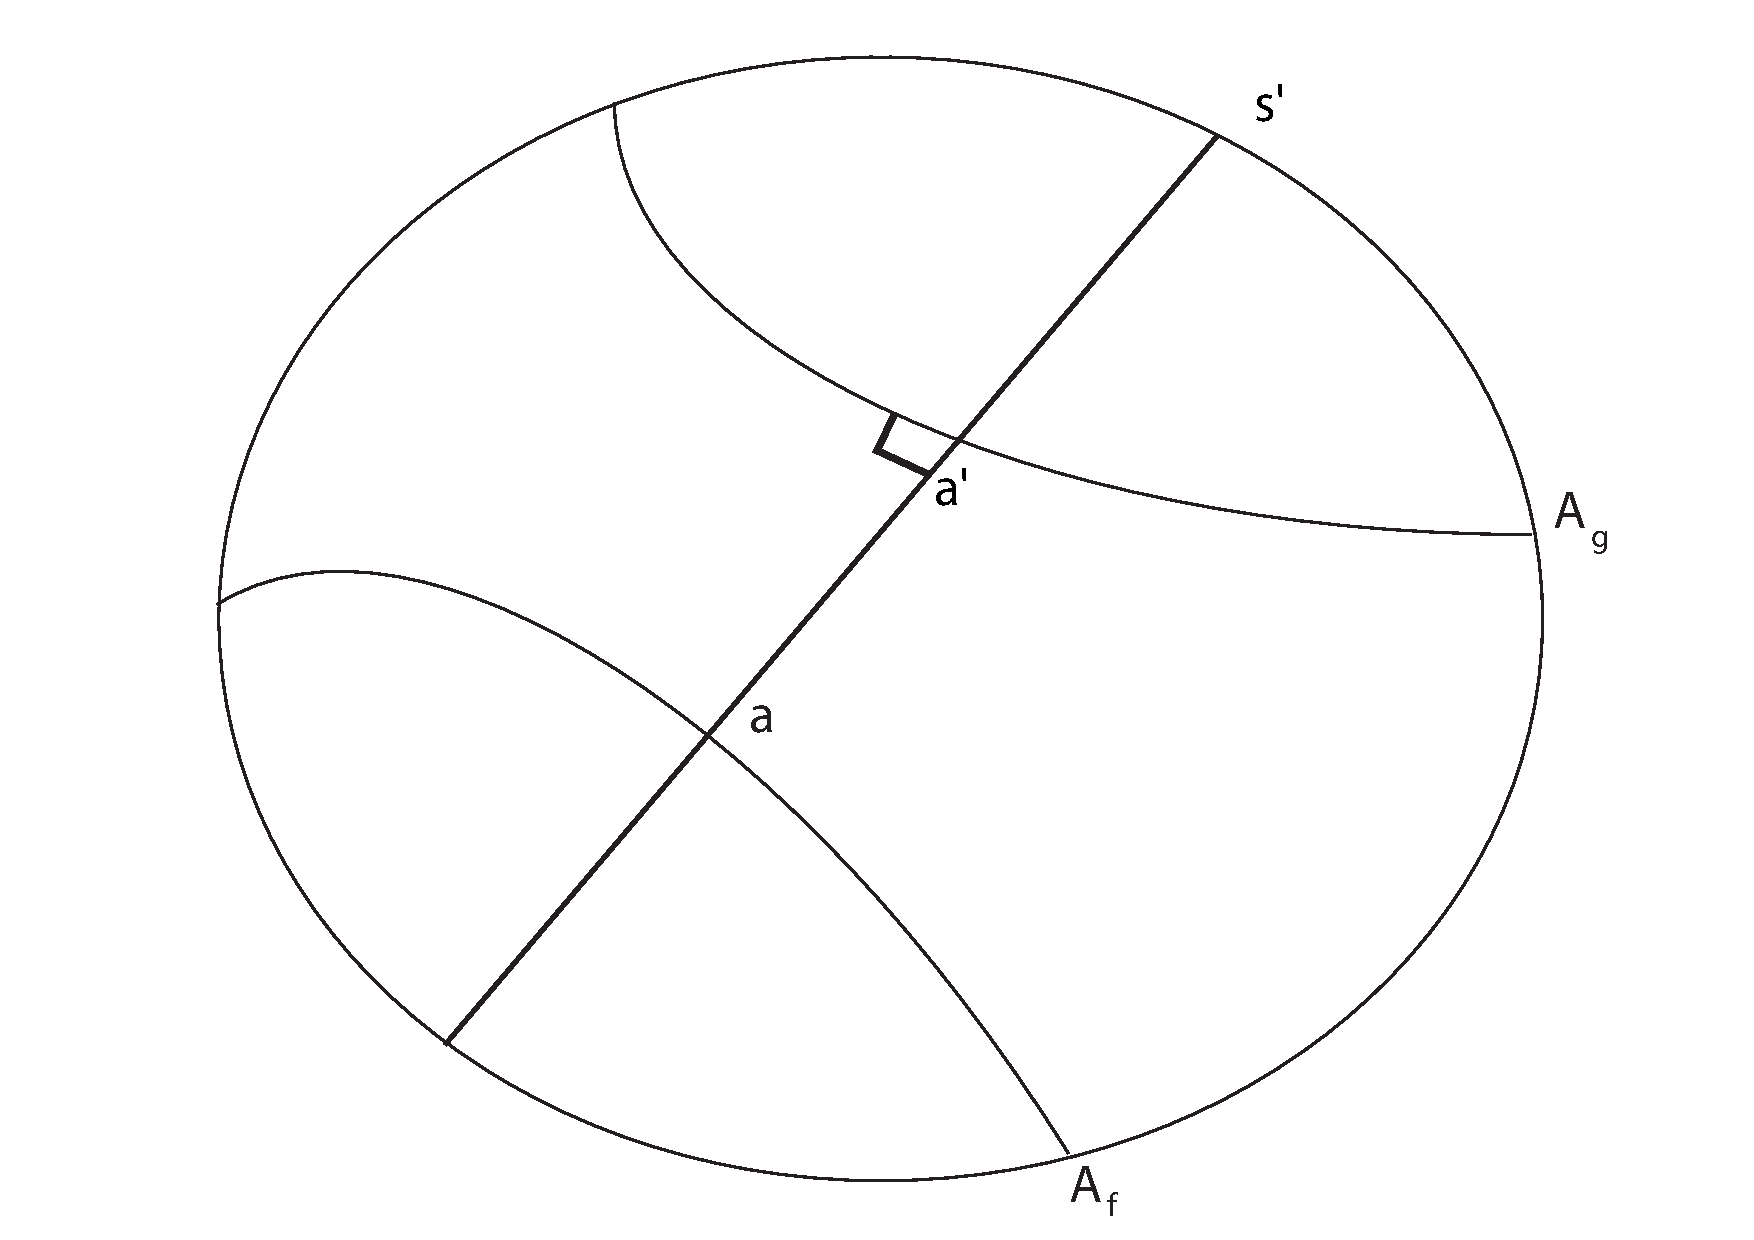
\includegraphics[width=10cm]{lemma1-dem1.pdf}\\
  \caption{Figura \ref{lemma1-dem1} }\label{lemma1-dem1}
\end{figure}


Queremos saber ahora que tipo de transformaci\'on es $fg$, por lo
anterior tenemos que $fg= ss's's'' = ss''$, ahora todo depende de la
posici\'on de los ejes de $f$ y $g$. \\ \\


\textbf{ Caso 1.}[las rectas se intersectan el alg\'un punto de
$D+E$] \\


Sea $m$ el punto medio del segmento $aa'$, la normal a $s'$ que
pasa por $m$ bisecta el \'angulo que forman los ejes en el punto de
intersecci\'on $p$ (\ref{lemma1-dibujo4}), para
ver esto reflejamos las rectas $l$ y $\sigma$ respecto de $l$
obtenemos $l$ y $s''$, como la reflexi\'on es conforme el \'angulo
entre $l$ y $s''$ es el mismo que el \'angulo entre $l$ y $s$. Es
claro que el punto de intersecci\'on $p$ sera el punto fijo de la
transformaci\'on, sea $\frac{1}{2} \phi_{fg}$ el \'angulo entre $s$
y $s'$ (la inversi\'on respecto a dos circunferencias es un elemento el\'iptico con \'angulo el doble del \'angulo de
esta interseccion). \\

\begin{figure}[h]
  \centering
  % Requires \usepackage{graphicx}
  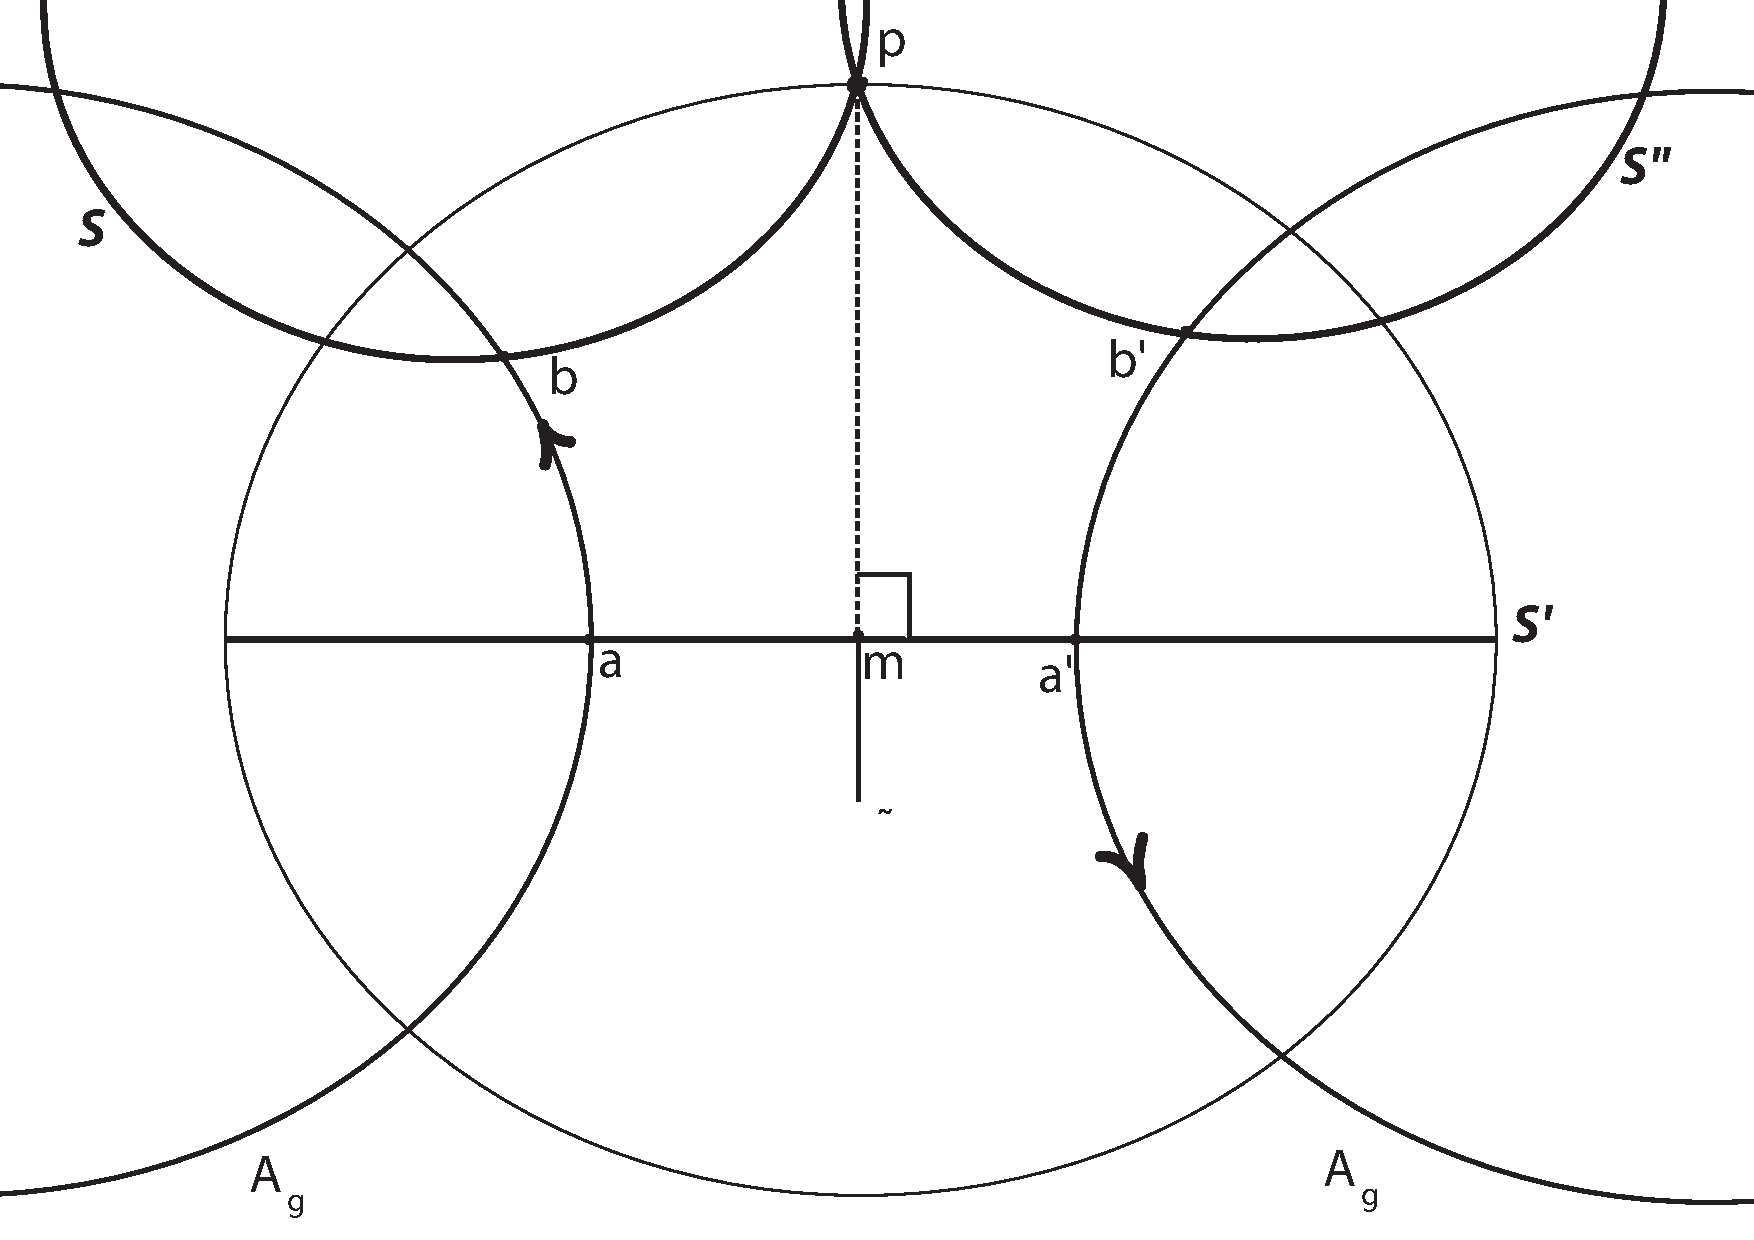
\includegraphics[width=10cm]{lemma1-dibujo4}\\
  \caption{Figura \ref{lemma1-dibujo4}}\label{lemma1-dibujo4}
\end{figure}



Luego $abpm$ es un cuadrilatero con 3 \'angulos rectos y el \'angulo
restante agudo (cuadrilatero de lambert Fig. \ref{lemma1-dibujo5}) cuyas medidas son
$\frac{1}{4} \phi_{fg}$ con lados $\frac{1}{2} \delta$ y $
\frac{1}{2} \lambda$ por lo cual tenemos $senh \frac{1}{2} \delta
senh \frac{1}{2} \lambda = cos \frac{1}{4} \phi_{fg} \leq 1$ y es
igual a 1 en el caso de que se intersecten en el infinito ( $\phi
=0$) y en dado caso la transformaci\'on seria parab\'olica. \\ \\

\begin{figure}[h]
  \centering
  % Requires \usepackage{graphicx}
  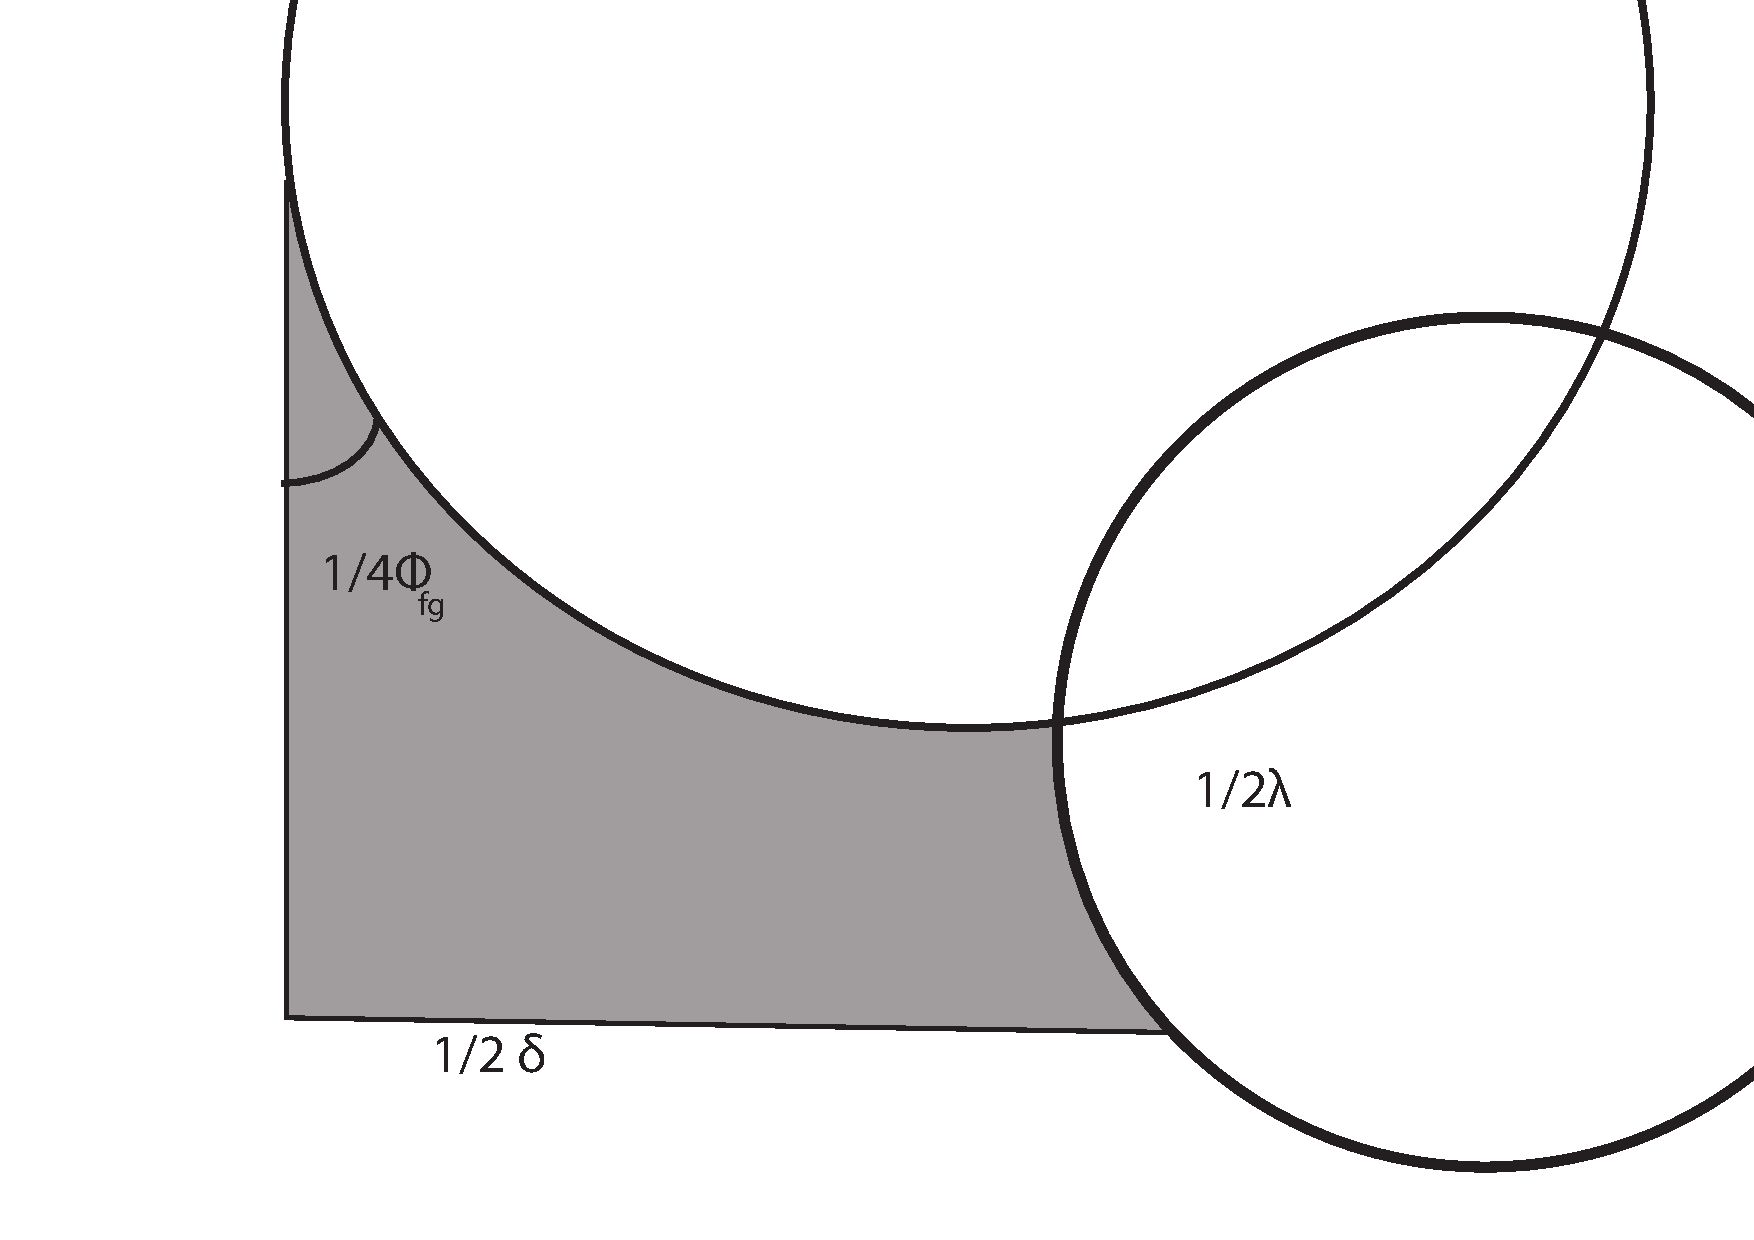
\includegraphics[width=10cm]{lemma1-dibujo5}\\
  \caption{Cuadrilatero de Lambert}  \label{lemma1-dibujo5}
\end{figure}



\textbf{Caso 2}


En el caso que los ejes sean divergentes, existe una recta normal a
ambos  y se tiene que la recta $l$ bisecta al segmento entre $s$ y
$s'$ de esta recta normal, entonces basta probar que;

\begin{enumerate}
\item Esta recta normal es el eje de $fg$
\item En efecto $l$ bisecta al segmento entre $s$ y $s'$ de esta
recta normal
\end{enumerate}

Para (1) Probaremos que $fg$ es hiperb\'olica viendo que tiene dos
puntos fijos y que se encuentran en la normal mencionada antes. Sean
$x$ y $x' $ los puntos finales de dicha recta normal y notemos que
$s''x=x'$ ya que $s''x$ debe cumplir que esta sobre la recta normal
a $s''$ y que $d_{H}(x,s'')=d_{H}(s''x,s'')$ pero $d_{H}(x,s'') =
\infty$, por la misma raz\'on $sx'=x$ entonces $ss''x=x$ y tambien
se cumple $ss''x'=x'$ por lo tanto $fg$ tiene 2 puntos fijos y su
eje es la recta que los une, que en este caso es la recta normal
mencionada (Fig. \ref{lemma1-dibujo6-2}).

\begin{figure}[h]
  \centering
  % Requires \usepackage{graphicx}
  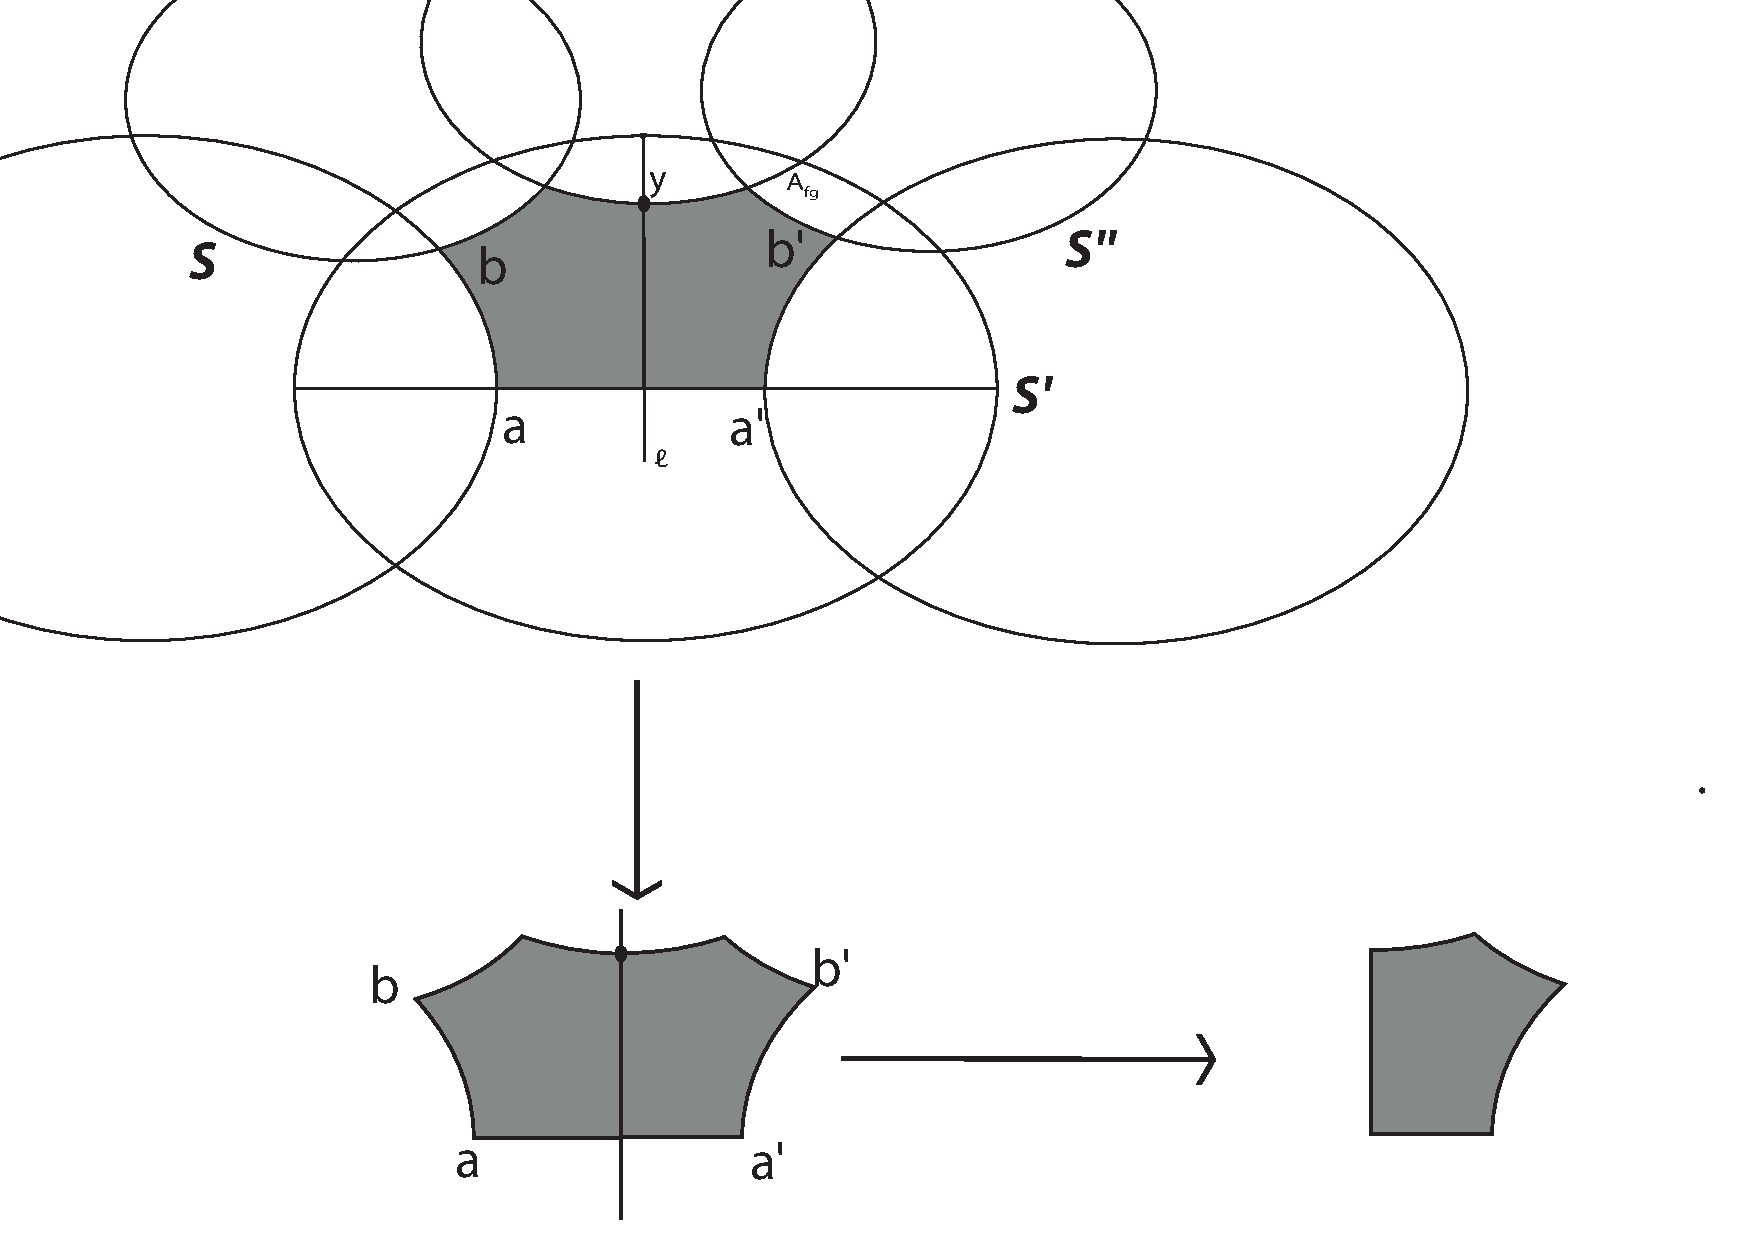
\includegraphics[width=10cm]{lemma1-dibujo6-2}\\
  \caption{Figura \ref{lemma1-dibujo6-2} }\label{lemma1-dibujo6-2}
\end{figure}


Para (2) queremos probar que $d_{H}(x,y) = d_{H}(y,x')$ donde $y$ es
el punto de intersecci\'on de la normal con $l$, al reflejar
respecto de $l$ y notando que $x \mapsto x'$ bajo $s$ y $d_{H}(x,y)
= d_{H}(y,sx)$ tenemos el resultado. \\


Finalmente tenemos las rectas $s'',A_{g},s,l$ y $A_{fg}$ y estas
forman un pentagono con 4 \'angulos rectos y con lados
$\frac{1}{2}\lambda_{fg},\frac{1}{2}\delta,\frac{1}{2}\lambda$
 (Fig. \ref{lemma1-dibujo9}) y podemos concluir (\ref{cha:apendice})
$$ senh \frac{1}{2} \delta senh \frac{1}{2} \lambda = cosh \frac{1}{4} \lambda_{fg} >1$$
$ _{\square} $

\begin{figure}[h]
  \centering
  % Requires \usepackage{graphicx}
  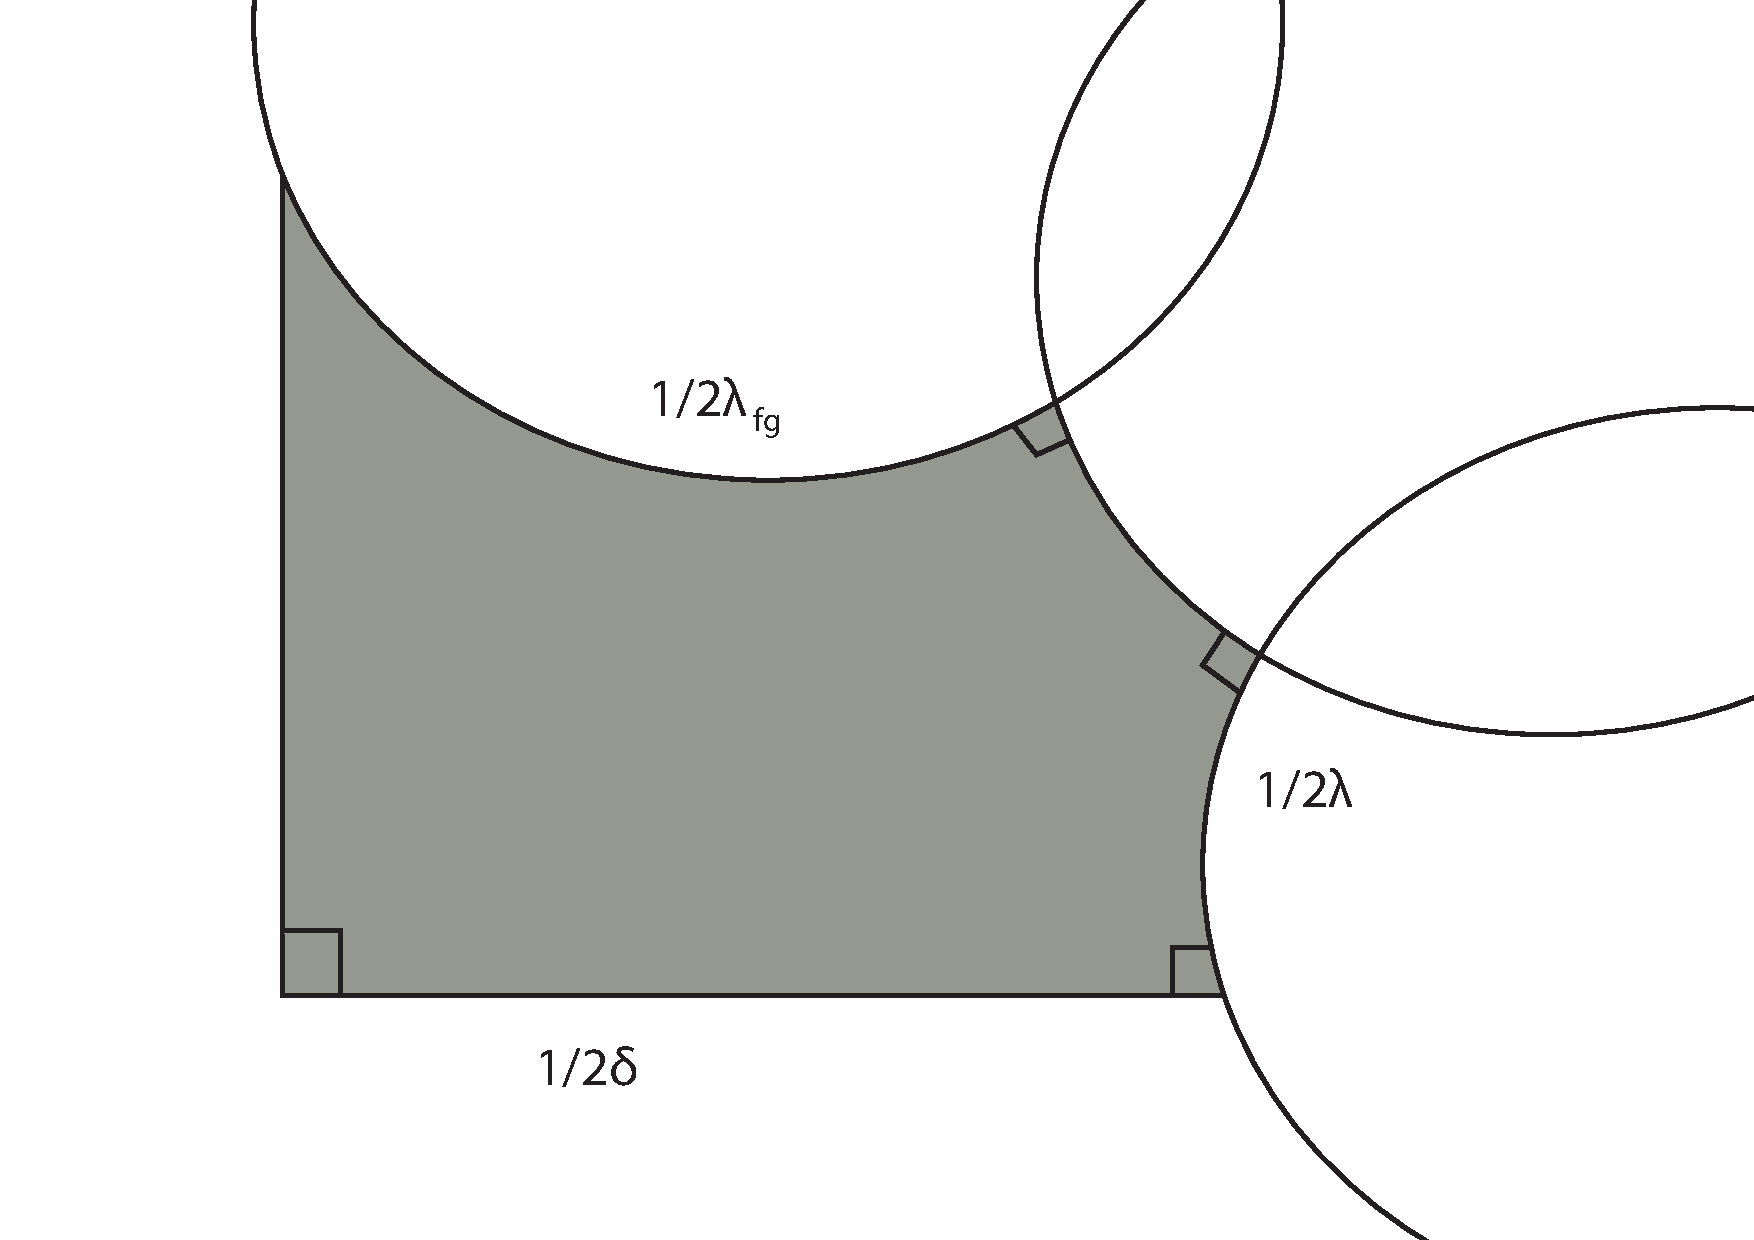
\includegraphics[width=10cm]{lemma1-dibujo9}\\
  \caption{Pent\'agono con 4 \'angulos rectos}\label{lemma1-dibujo9}
\end{figure}



\section{El lema del conmutador de los elemetos hiperb\'olicos}

\begin{lem} \label{lema2}
Sean $f$ y $g$ dos elementos hiperb\'olicos con ejes $A_{f}$ y
$A_{g}$ y desplazamientos iguales $\lambda $, y con \'angulo de
intersecci\'on $\phi $.El conmutador $[f,g]=fgf^{-1}g^{-1}$
es el\'iptico , parab\'olico o hiperb\'olico dependiendo de

$$ senh^{2}(\frac{1}{2} \lambda) sen \phi  \left \{ \begin{matrix} >1
\\ =1 \\ < 1 \end{matrix}\right. $$
\end{lem}

\textit{Prueba}:

Sea $s'$ el punto de intersecci\'on de $A_{f}$  y $A_{g}$, sea $s$
el punto sobre $A_{f}$ tal que $d_{H}(s',s)= \frac{1}{2} \lambda$ y
trazado siguiendo la direcci\'on de $A_{f}$, y sea $s''$ el punto
sobre $A_{g}$ tal que $d_{H}(s',s'')=\frac{1}{2} \lambda$ y trazado
siguiendo la misma direcci\'on que $A_{g}$ (Fig. \ref{lemma2-dibujo1}). \\

\begin{figure}[h]
  \centering
  % Requires \usepackage{graphicx}
  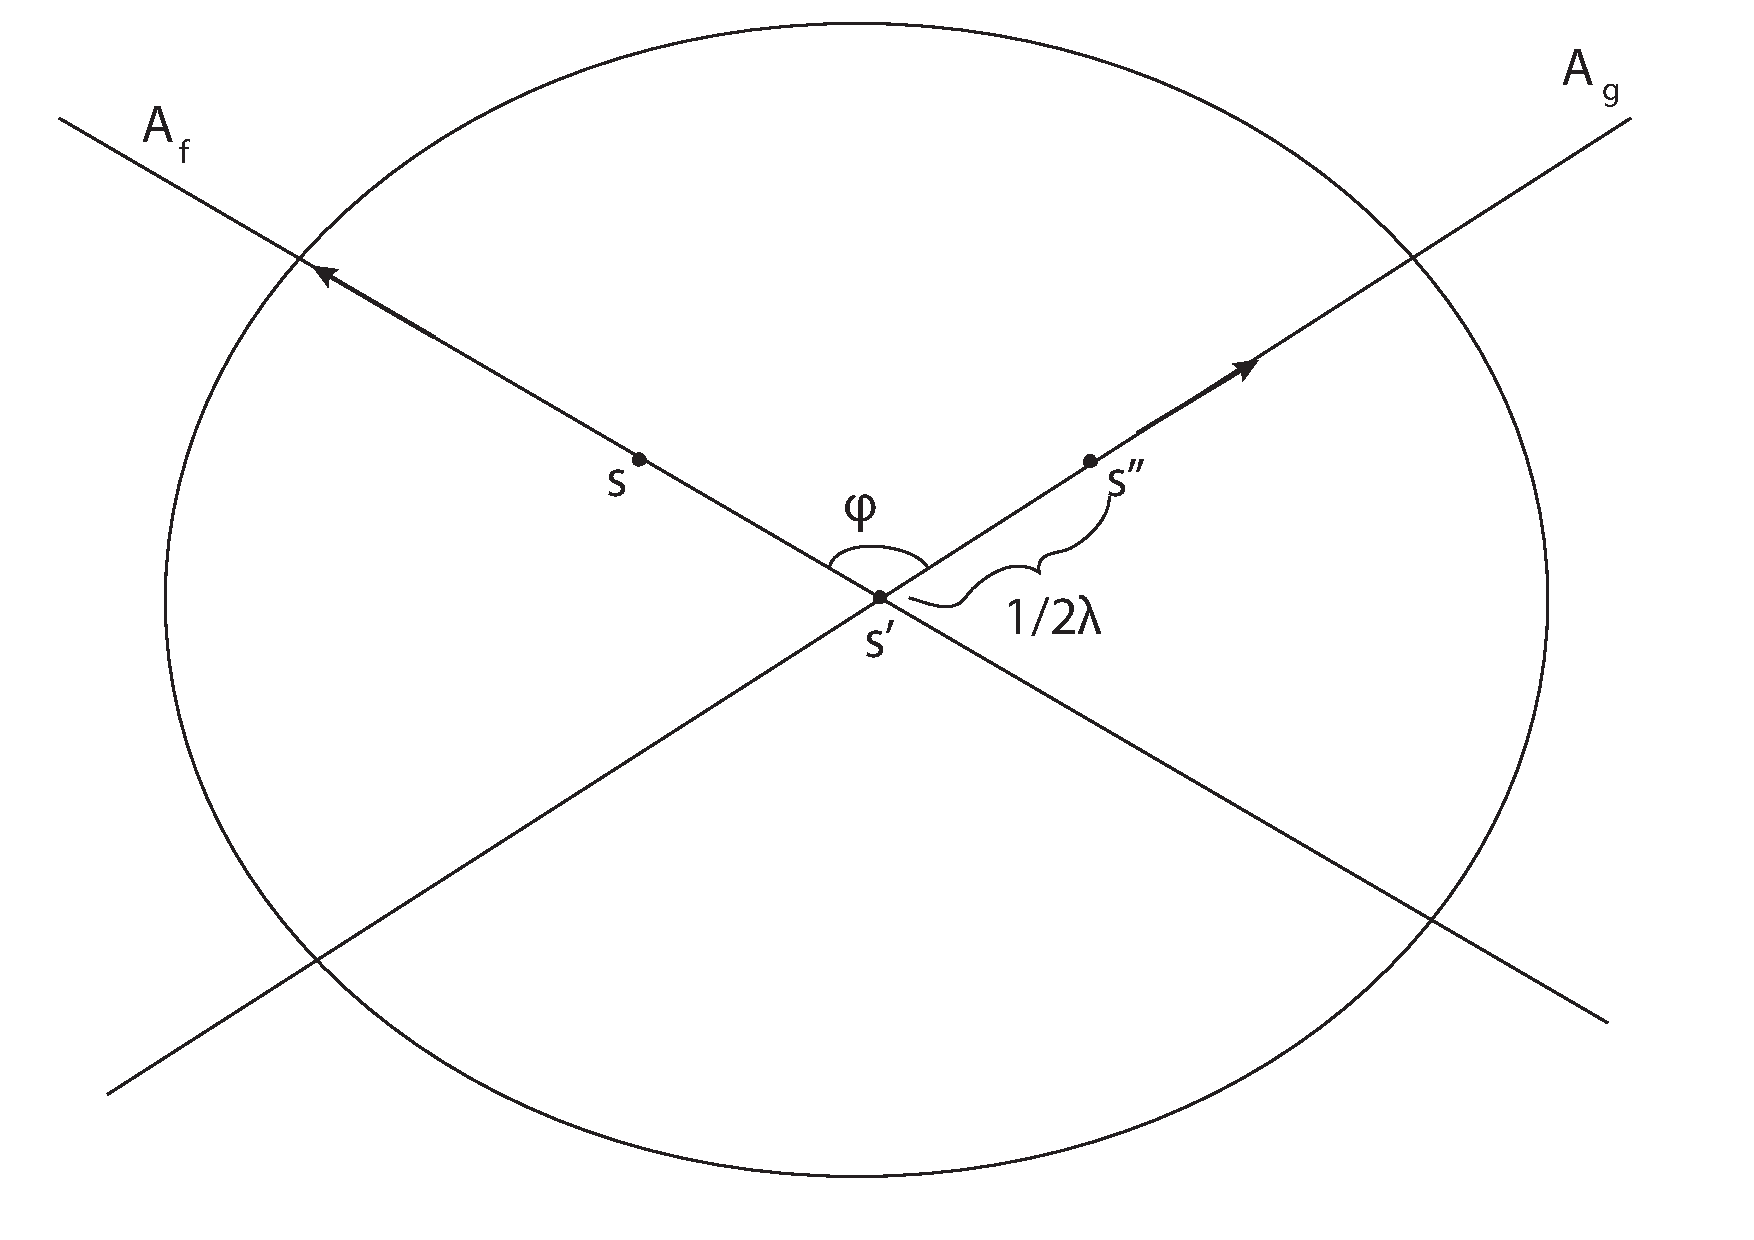
\includegraphics[width=10cm]{lemma2-dibujo1}\\
  \caption{Figura \ref{lemma2-dibujo1}}\label{lemma2-dibujo1}
\end{figure}


Y consideremos los elementops el\'ipticos de \'angulo $\pi$  respecto a estos puntos
y los denotaremos igual que denotamos a sus puntos fijos. \\

Queremos primero probar que $f=ss'$, para esto deseamos ver los puntos que deja fijos $ss'$. El elemento el\'iptico con \'angulo $\pi$ funciona de la
siguiente manera; dado un punto $x$ se traza la recta que va de $x$
al punto fijo $c$,la im\'agen de $x$ bajo el elemento el\'iptico llamemosle $y$ esta
sobre la misma recta y $d_{H}(x,c)=d_{H}(y,c)$, con este proceso
podemos ver que $ss'$ fija los mismos puntos que $f$ por lo tanto el
eje de $f$ es el mismo que el  de $ss'$ solo falta ver cuanto es el
desplazamiento de $ss'$,como antes, basta verificarlo para un
punto y en esta ocasi\'on tomamos el punto $s'$, tenemos que
$d_{H}(s,ss'(s'))=d_{H}(s,s(s'))= 2d_{H}(s',s)=2(\frac{1}{2}
\lambda)= \lambda $ por lo tanto $f=ss'$. Un proceso an\'alogo nos
enseña que $g=s's''$ y como $s's'$ es la indentidad entonces $fg
= ss''$, m\'as a\'un $f^{-1} = s's,g^{-1}=s''s'$ y entonces
$f^{-1}g^{-1}= s'ss''s'=s'fgs'=s'fgs'^{-1}$, luego $ss'$ es un
elemento hiperb\'olico con recta invariante igual a la recta que pasa por
$s$ y $s''$ y desplazamiento $2d_{H}(s,s'')$, m\'as a\'un
$f^{-1}g^{-1}$ es hiperb\'olico obtenido de $fg$ conjungando por
$s'$, tenemos entonces;

\begin{enumerate}
\item $f^{-1}g^{-1}$ tiene un desplazamiento con la misma medida que
$fg$
\item su eje $A_{f^{-1}g^{-1}}$ se obtiene de $A_{fg}$ rotando por $s'$.
\end{enumerate}

Para probar (1) queremos ver cuanto mide $d_{H}(x,s'fgs'x)$ y
tenemos que $d_{H}(x,s'fgs'x)= d_{H}(s'x,fg(s'x))$ y esta \'ultima
cantidad es el desplazamiento de $fg$. \\ \\

(2) se cumple  ya que $f^{-1}g^{-1} (s'A_{fg})= s'fgs'(s'A_{fg})=
s'fg(A_{fg})=s'A_{fg}$. \\

Entonces estos ejes son divergentes y sus correspondientes
transformaciones tienen sentidos opuestos, aplicamos entonces el
\textbf{lema} \ref{lema1} a $fg$ y a $f^{-1}g^{-1}$ entonces $[f,g]$ es
el\'iptico , parab\'olico o hiperb\'olico seg\'un sea

$$senh \eta senh \frac{1}{2} \lambda_{fg} \lesseqgtr 1$$

Donde $\eta$ es la perpendicular desde $s'$ en el tri\'angulo
$ss's''$ (Fig. \ref{lemma2-dibujo4}) y por trigonometr\'ia hiperb\'olica (\ref{cha:apendice}) se cumple $senh \eta
senh\frac{1}{2} \lambda_{fg} = sen \phi senh^{2} \frac{1}{2}\lambda$
$_{\square}$

\begin{figure}[h]
  \centering
  % Requires \usepackage{graphicx}
  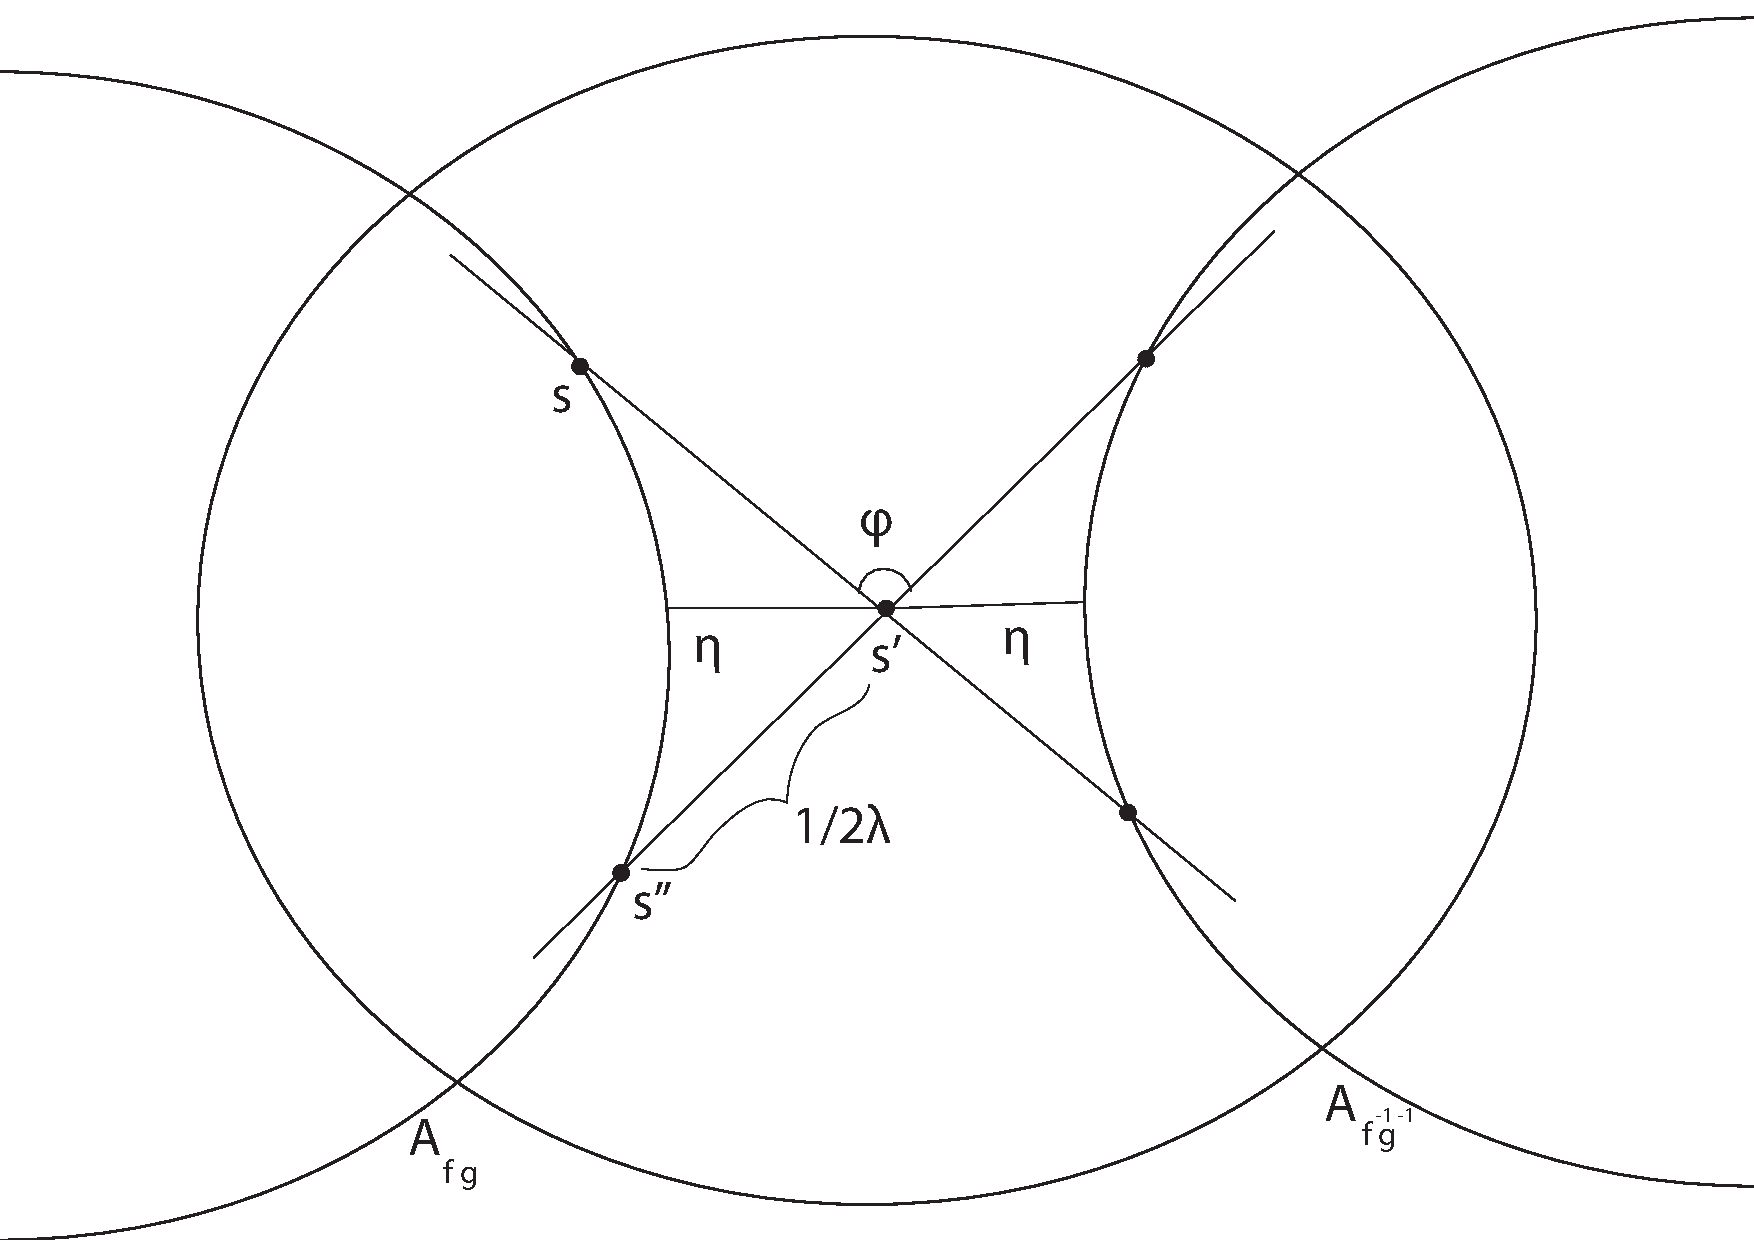
\includegraphics[width=7cm]{lemma2-dibujo4}\\
  \caption{Figura \ref{lemma2-dibujo4}}\label{lemma2-dibujo4}
\end{figure}


\section{El lema del conmutador de los elementos parab\'olicos}

\begin{lem}\label{lema3}
Sean $f,g$ elementos parab\'olicos con puntos fijos $c_{f}$ y
$c_{g}$ entonces el conmutador $[f,g]$ es hiperb\'olico.
\end{lem}

\emph{Prueba.} \\

\begin{figure}[h]
  \centering
  % Requires \usepackage{graphicx}
  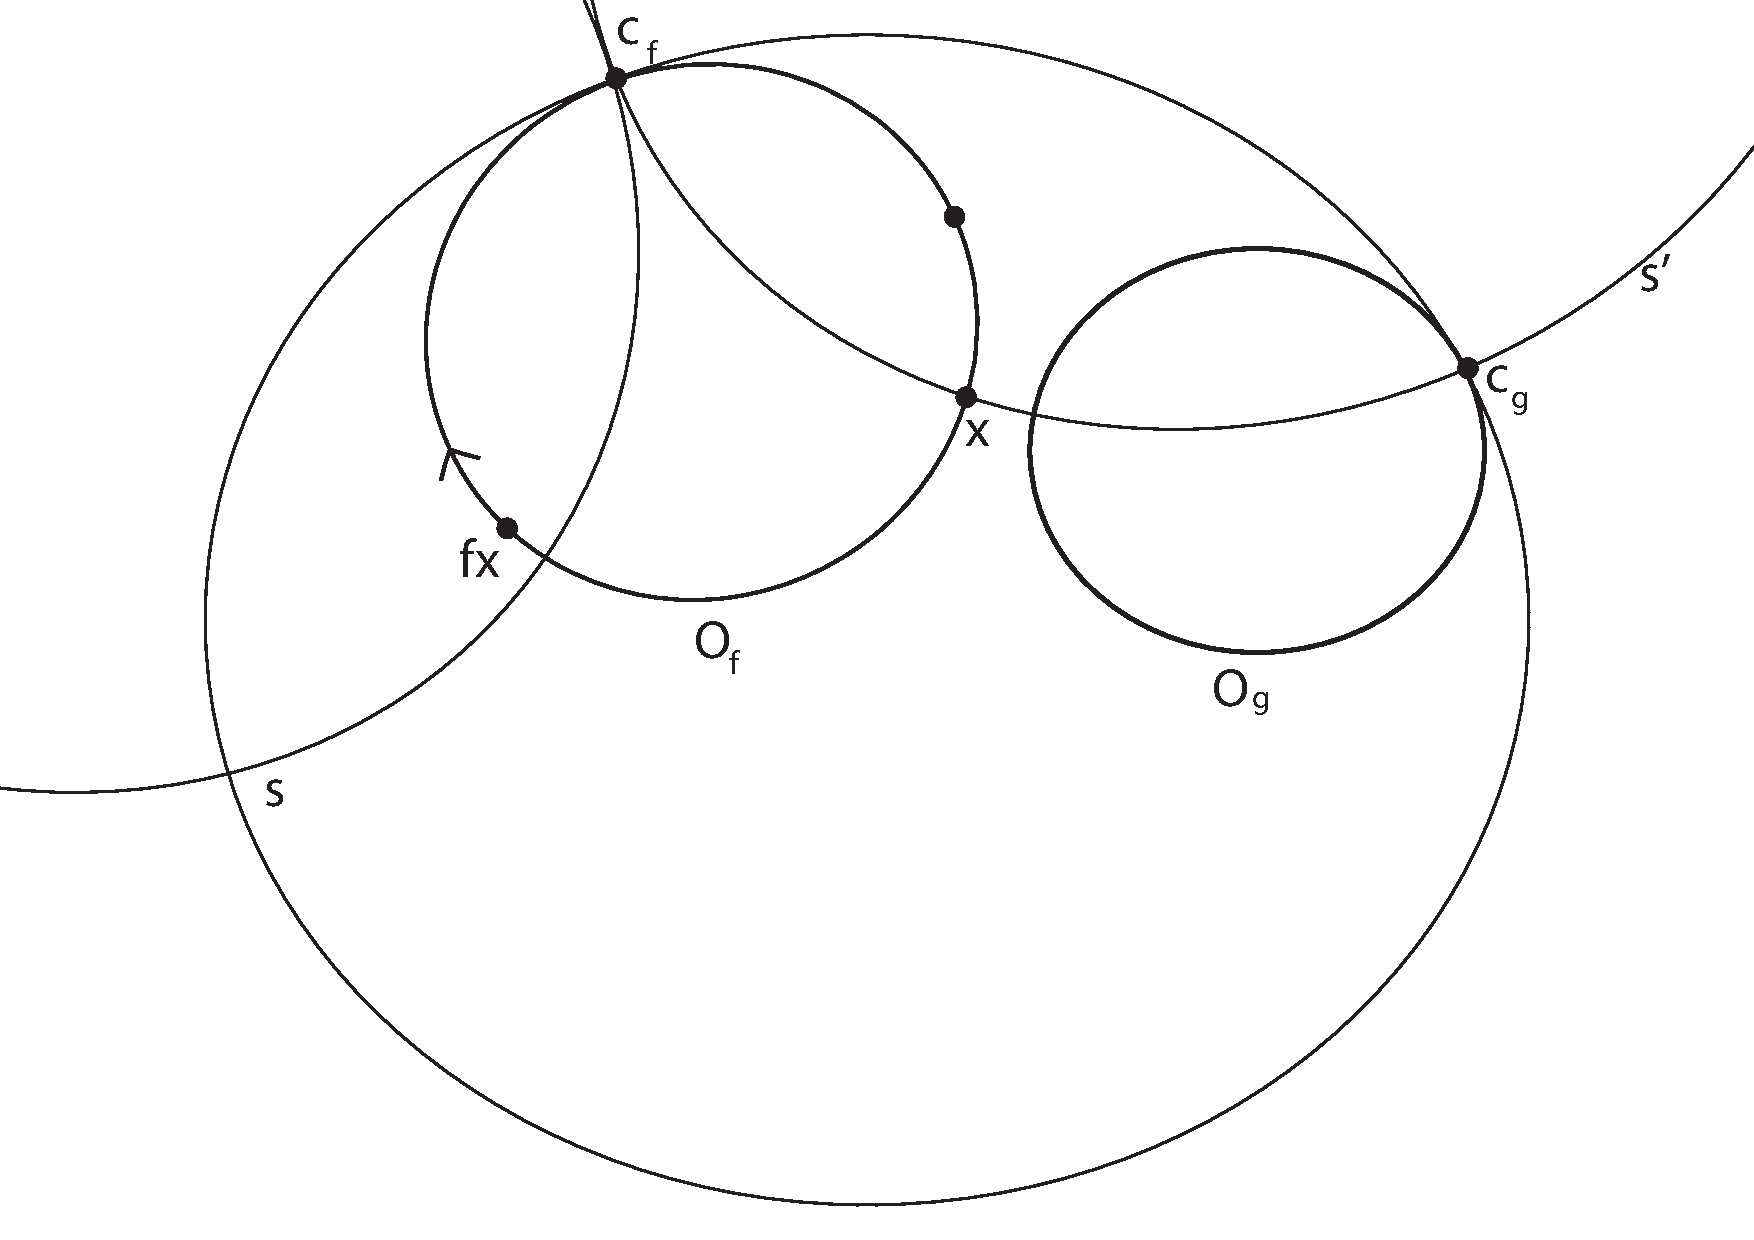
\includegraphics[width=10cm]{lemma3-dibujo1}\\
  \caption{Figura \ref{lemma3-dibujo1}}\label{lemma3-dibujo1}
\end{figure}


 Sea $s'$ la recta que une $c_{f}$ y $c_{g}$ y denotemos la reflexi\'on respecto a esta recta
tambi\'en como $s'$. Sea $O_{f}$ un horociclo dado con punto al
infinito $c_{f}$, y $x \in O_{f}$, tomamos $s$ en el conjunto de geod\'esicas que pertenece al haz parab\'olico con punto fijo $c_{f}$ (\cite{Beardon}).

Tenemos entonces que $ f=ss' $, y analogamente obtenemos  que existe
$s''$ tal que $g=s's''$ luego tenemos
$[f,g]=ss''s'ss''s'=(ss''s')^{2}$, la composici\'on de reflexiones
conserva el sentido por lo tanto la composici\'on de 3 reflexiones
invierte el sentido y es por tanto una reflexi\'on o una
h-reflexi\'on entonces su cuadrado es la identidad o un elemento
hiperb\'olico.Probemos que  $f$ y $g$ no permutan: Si $fg=gf$, tenemos que $f$ deja invariante el conjunto de puntos fijos de $g$ y vicerversa, para ver esto sea $x$ un punto fijo de $f$ entonces $f(g(x))= g(f(x)) = g(x)$, es decir $g(x)$ es un punto fijo de $f$, si sustituimos $g$ por $g^{-1}$ analogamente obtenemos que $g^{-1}(x)$ es un punto fijo, es decir todo punto fijo es la imagen bajo $g$ de otro punto fijo ( $x= g(g^{-1}(x))$). Dado esto $[f,g]$ es la identidad si y solo si $f$ y $g$ conmutan, como hemos probado que esto no es posible se tiene que $[f,g]$ es un elemento hiperb\'olico. $_{\square}$

\section{El lema del conmutador de los elementos hiperb\'olicos con ejes paralelos}

\begin{lem} \label{lema4}
Sean $f$ y $g$ elementos hiperb\'olicos con ejes paralelos y con
punto com\'un $u$, entonces el conmutador $[f,g]$ es un elemento
parab\'olico con centro en $u$
\end{lem}

\begin{figure}[h]
  \centering
  % Requires \usepackage{graphicx}
  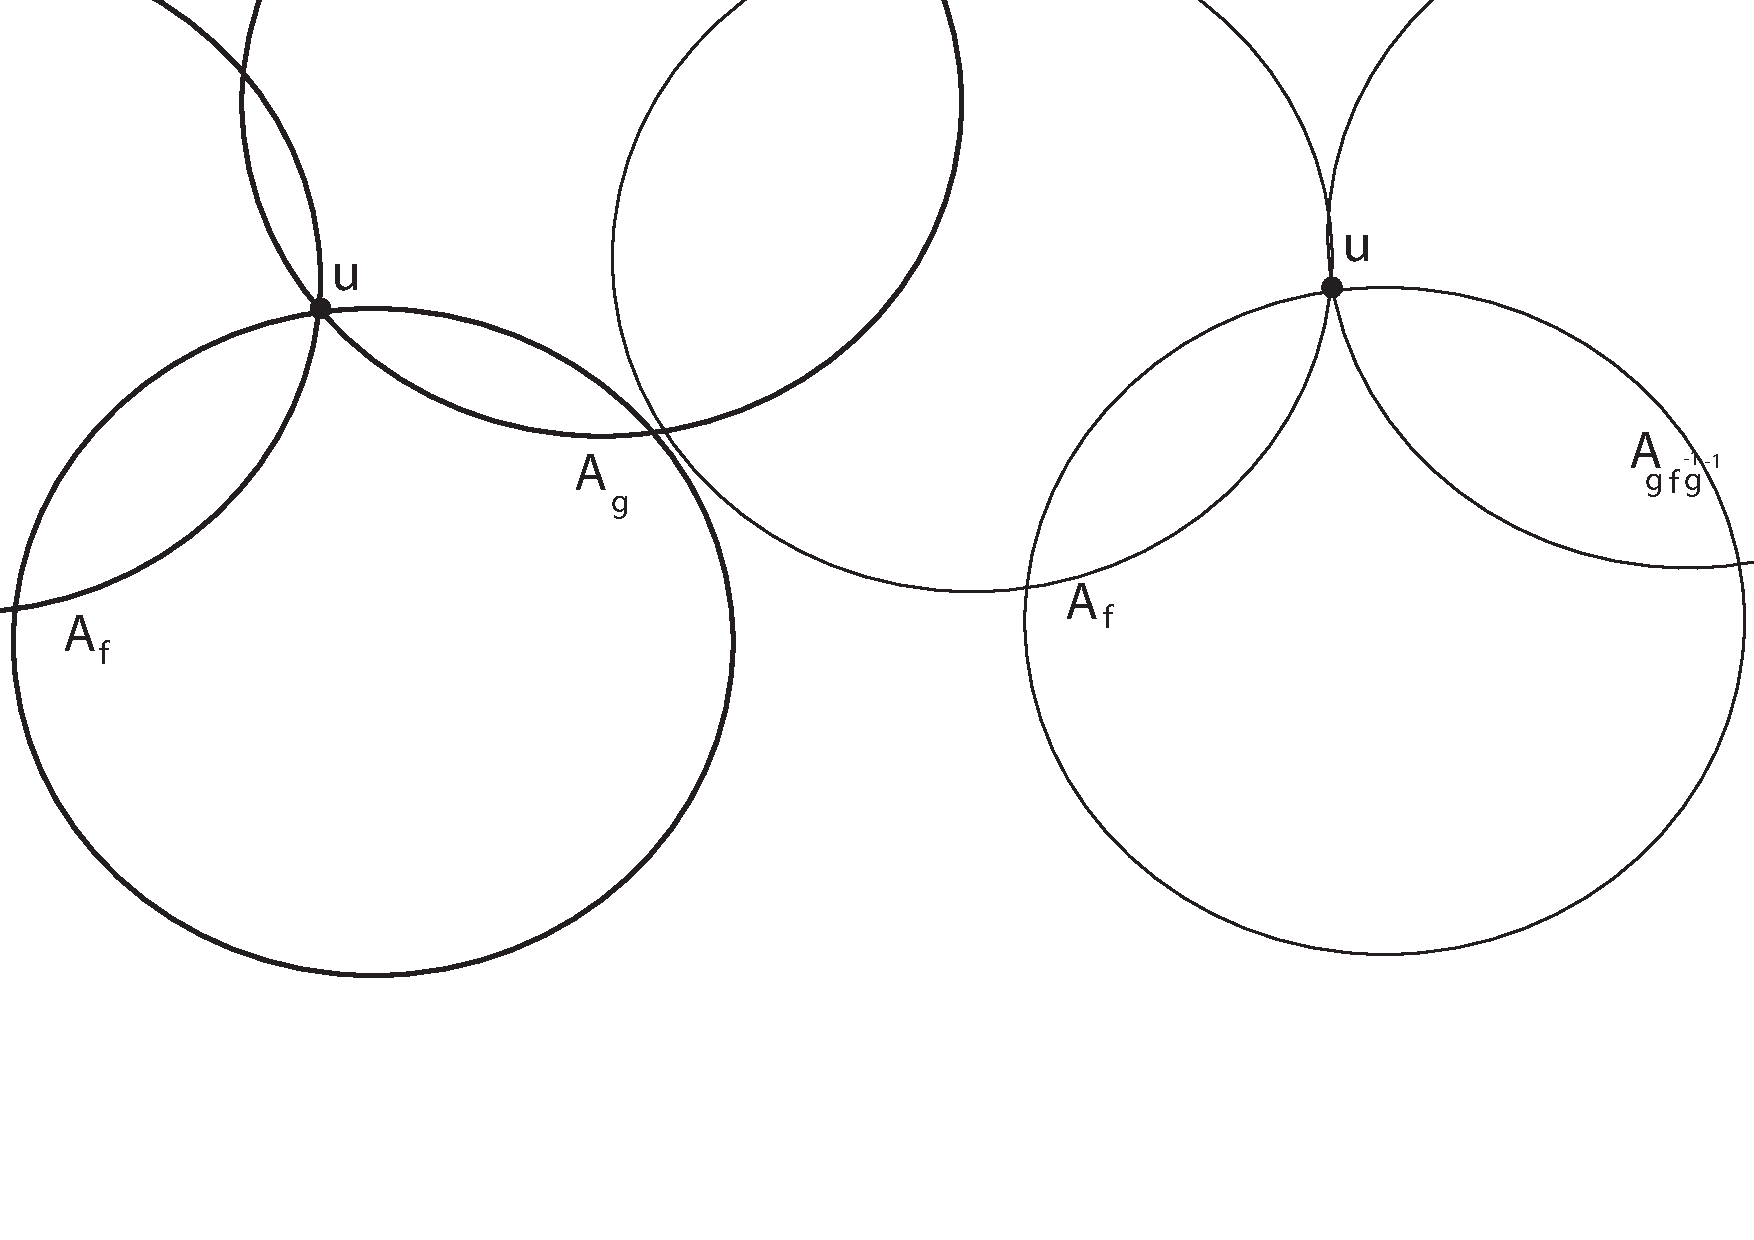
\includegraphics[width=10cm]{lemma4-dibujo1}\\
  \caption{Figura \ref{lemma4-dibujo1}}\label{lemma4-dibujo1}
\end{figure}



\textit{Prueba}:

Primero veamos que  $f \neq gf^{-1}g^{-1}$, es claro que
$gf^{-1}g^{-1}$ fija $u$ ya que tanto $f$ como $g$ lo fijan, sea $x$
el punto final del eje de $f$ distinto de $u$, es claro que $g^{-1}$
no fija este punto, y $gx \neq u$ (puesto que $g^{-1}u \neq x$)
concluimos con esto $f \neq gf^{-1}g^{-1}$.

Sin perdida de generalidad podemos suponer que $u=0$ y que las matrices de los elementos hiperb\'olicos correspondientes a $f$ y $g$ lucen de la siguiente manera:

$$M_{f}=    \begin{pmatrix}
 a& 0\\
 c & d
 \end{pmatrix} \  ,  \ M_{g} =     \begin{pmatrix}
 x& 0\\
 w& z
 \end{pmatrix}   $$

 Donde $ad=1,xz=1$ , $|a+d|>2$ y $|x+z|>2$. Haciendo los c\'alculos obtenemos que $tr (M_{f}M_{g}M_{f^{-1}}M_{g^{-1}})=2$ por lo que el conmutador es un elemento parab\'olico con punto fijo $u=0$. $_{\square}$

%Primero veamos que  $f \neq gf^{-1}g^{-1}$, es claro que
%$gf^{-1}g^{-1}$ fija $u$ ya que tanto $f$ como $g$ lo fijan, sea $x$
%el punto final del eje de $f$ distinto de $u$, es claro que $g^{-1}$
%no fija este punto, y $gx \neq u$ (puesto que $g^{-1}u \neq x$)
%concluimos con esto $f \neq gf^{-1}g^{-1}$, claramente su
%desplazamiento mide lo mismo (debido a que $g$ es isometria) pero
%con sentidos opuestos (ya que $gf^{-1}g^{-1}$ respeta el sentido de
%$f^{-1}$). (\textcolor[rgb]{1.00,0.00,0.00}{dibujo})
%(\textcolor[rgb]{0.00,0.00,1.00}{inconcluso}).

\section{El lema del elemento el\'iptico}

\begin{lem} \label{lema5}
Si en un grupo $G < PSL(2,\mathbb{R})$ sin puntos invariantes, 2
ejes de elementos hiperb\'olicos son paralelos entonces el grupo
contiene un elemento el\'iptico
\end{lem}


\textit{Prueba}:


Del Lema \ref{lema4} tenemos que $G$ contiene elementos parab\'olicos
y con punto en com\'un $u$ como centro. \\

Consideremos un Horociclo $K$ con punto en el infinito $u$, sobre $K$
el elemento parab\'olico tiene un desplazamiento fijo . \\

\begin{figure}[h]
  \centering
  % Requires \usepackage{graphicx}
  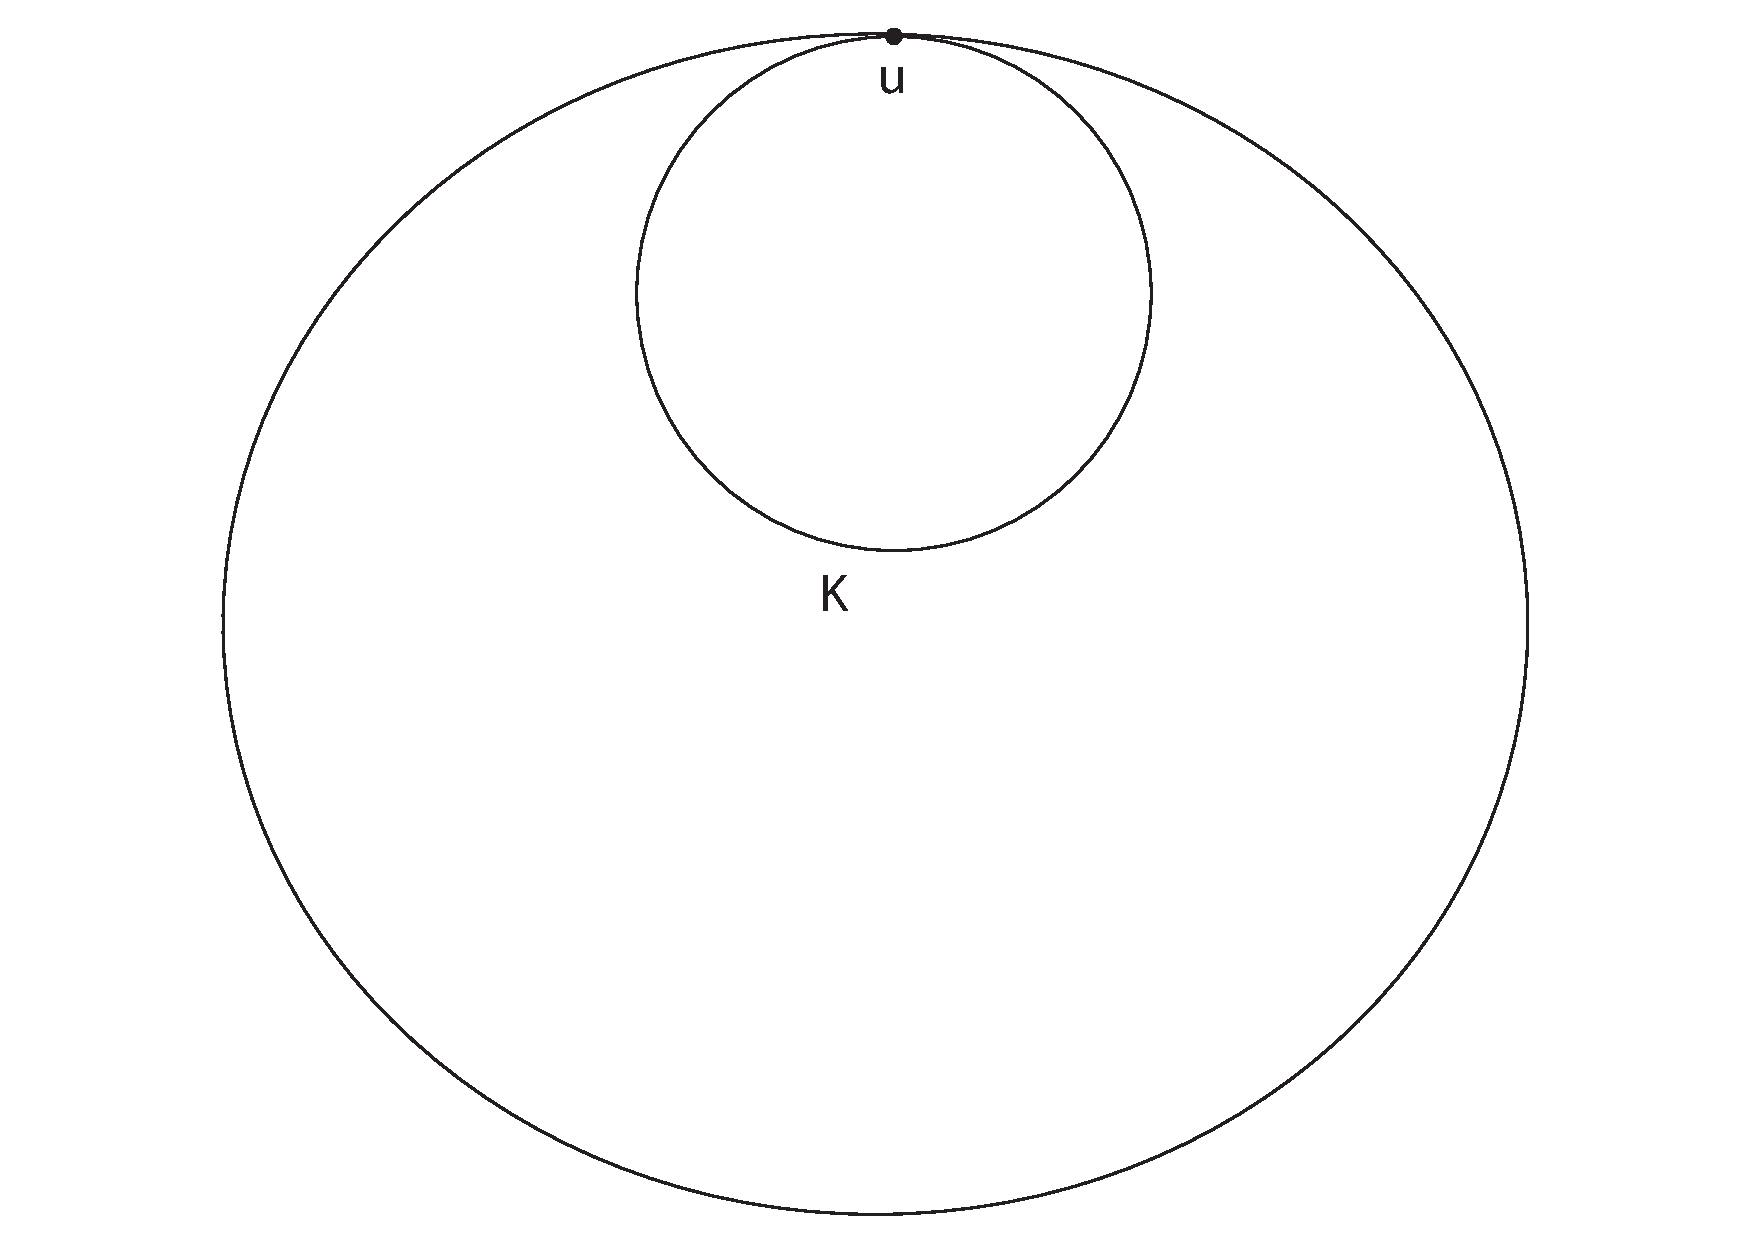
\includegraphics[width=10cm]{lemma5-dibujo1}\\
  \caption{Figura \ref{lemma5-dibujo1}}\label{lemma5-dibujo1}
\end{figure}


Sea $S_{u} < G$ el subgrupo de $G$ que consta de elementos
parab\'olicos con punto en el infinito $u$ y sea $x \in K$, la clase
de equivalencia $S_{u}x$ es un subconjunto de $K$ y podemos
distinguir dos casos.

\begin{enumerate}
\item Los puntos forman una sucesi\'on de puntos equidistantes
cuando $S_{u}$ es dinscontinuo.

\item El conjunto de puntos es denso en todo $K$ cuando $S_{u}$ no
es discontinuo.
\end{enumerate}

Para probar (1), sea $d=min \lbrace d_{H}(x,fx) | f \in S_{u}
\rbrace$ este minimo existe por que si no es asi se tendria un punto
de acumulaci\'on lo cual por hip\'otesis no es posible. Si $y \in
S_{u}x $ es claro que $min \lbrace d_{H}(y,fy) | f \in S_{u} \rbrace
= d$ y de esto concluimos que el conjunto de puntos es equidistante
de distancia $d$. \\

Para el caso (2) por hip\'otesis tenemos que $S_{u}x$ se acumula en
$x$ y queremos ver que se acumula en todo $K$. Sea $k \in K$ un
punto arbitrario y $B_{\epsilon}(k)= \lbrace z \in D| d_{H}(k,z) < \epsilon
\rbrace$ y tomemos $B_{\epsilon}(k) \cap K$, queremos ver que esxiste $x
\in S_{u}x$ tal que $d_{H}(k,x) < \epsilon$ , si dicha $x$ no existe
entonces los desplazamientos  en $K$ de los elementos de $S_{u}$
estarian acotados inferiormente por $\epsilon$ lo cual implicar\'ia que
$S_{u}$ es discontinuo lo que contradice la hip\'otesis, por lo
tanto $S_{u}$ en denso en todo $K$. \\

Ahora supongamos que estamos en el caso (1) y sea $g_{0}$ el
elemento con el menos desplazamiento respecto de $K$
(Fig. \ref{lemma5-dibujo2}) y $f$ un elemento
hiperb\'olico en $G$ tal que su eje $A_{f}$ tiene a $u$ como punto
fijo y cuyo sentido es tal que se aleja de $u$, entonces $fg_{0}f^{-1}$
fija $u$ y es un elemento parab\'olico y por tanto $fg_{0}f^{-1} \in
S_{u}$. \\

\begin{figure}[h]
  \centering
  % Requires \usepackage{graphicx}
  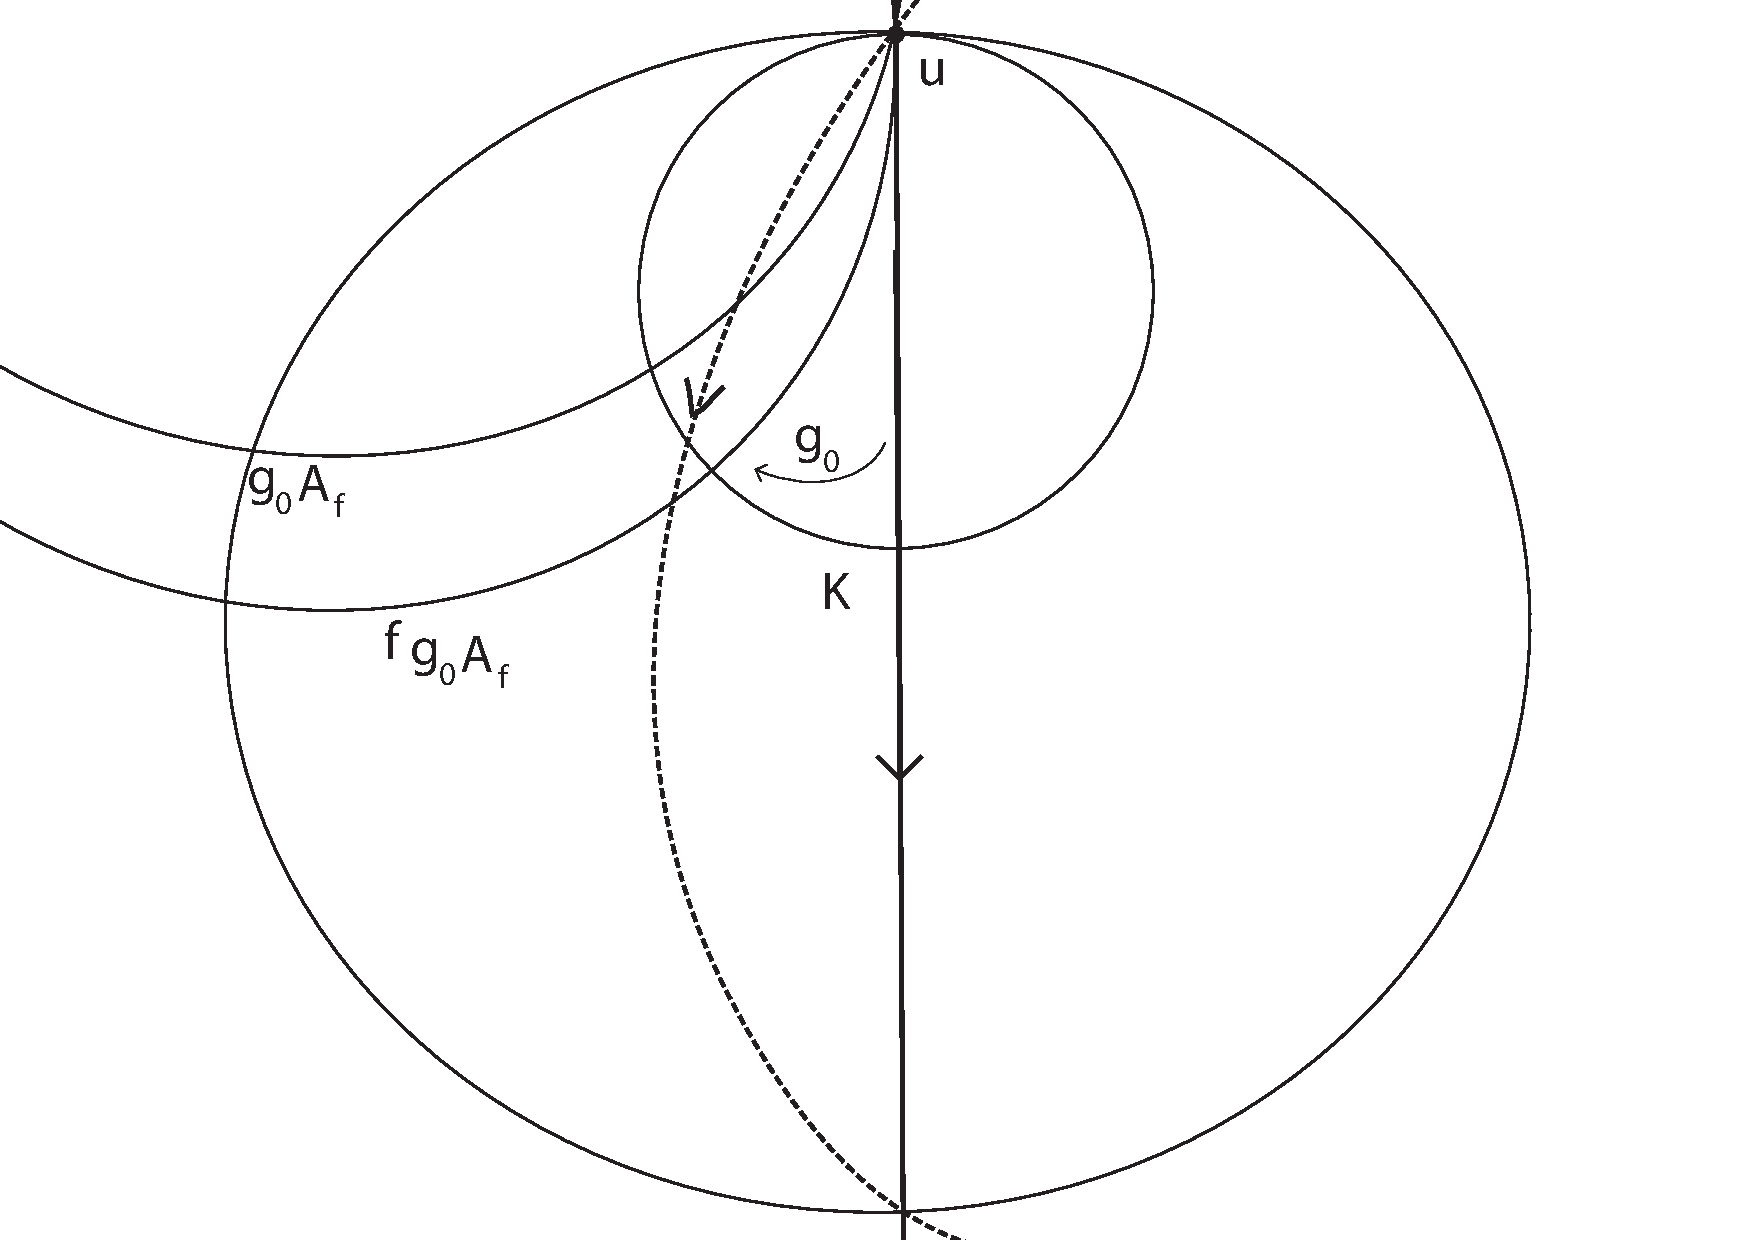
\includegraphics[width=10cm]{lemma5-dibujo2}\\
  \caption{Hiperciclo punteado }\label{lemma5-dibujo2}
\end{figure}

La imagen de $A_{f}$ bajo $fg_{0}f^{-1}$ es claramente la misma que
la de su imagen bajo $fg_{0}$, la recta $fg_{0}A^{f}$ se encuentra
entre $A_{f}$ y $g_{0}A_{f}$, luego el desplazamiento de $fg_{0}f^{-1}$
es menor que el de $g_{0}$ lo cual es una contradicci\'on, por lo
tanto $S_{u}x$ es denso en $K$, es decir los desplazamientos de los
elementos de $S_{u}$ son tan pequeños como se quiera. \\


Como $G$ no tiene a $u$ como punto invariante, sea $g \in G$ tal que
$gu \neq u$. Sean $f_{1},f_{2}$ elementos hiperb\'olicos
pertenecientes a los dos ejes del lema, al menos uno de los
elementos hiperb\'olicos $gf_{j}g^{-1}$ no fija $u$, ya
que $g$ solo puede mover $u$ a los m\'as a uno de los puntos
extremos de $A_{f_{j}}$. Entonces existe en $G$ un elemento
hiperb\'olico $f$ que no deja $u$ invariante. Elijamos ahora un
horociclo $K$ tal que intersecte $A_{f}$ (fig \ref{lemma5-dibujo3}) y elegimos $h$ tal que su
desplazamiento respecto a $K$ ayude a que los ejes $A_{f}$ y
$A_{hf}$ de $f$ y $f'=hfh^{-1}$ respectivamente se intersecten en un
\'angulo arbitrariamente pequeño, en particular elegimos $h$ tal
que
$$sen\phi senh^{2} \frac{1}{2} \lambda_{f} < 1$$

\begin{figure}[h]
  \centering
  % Requires \usepackage{graphicx}
  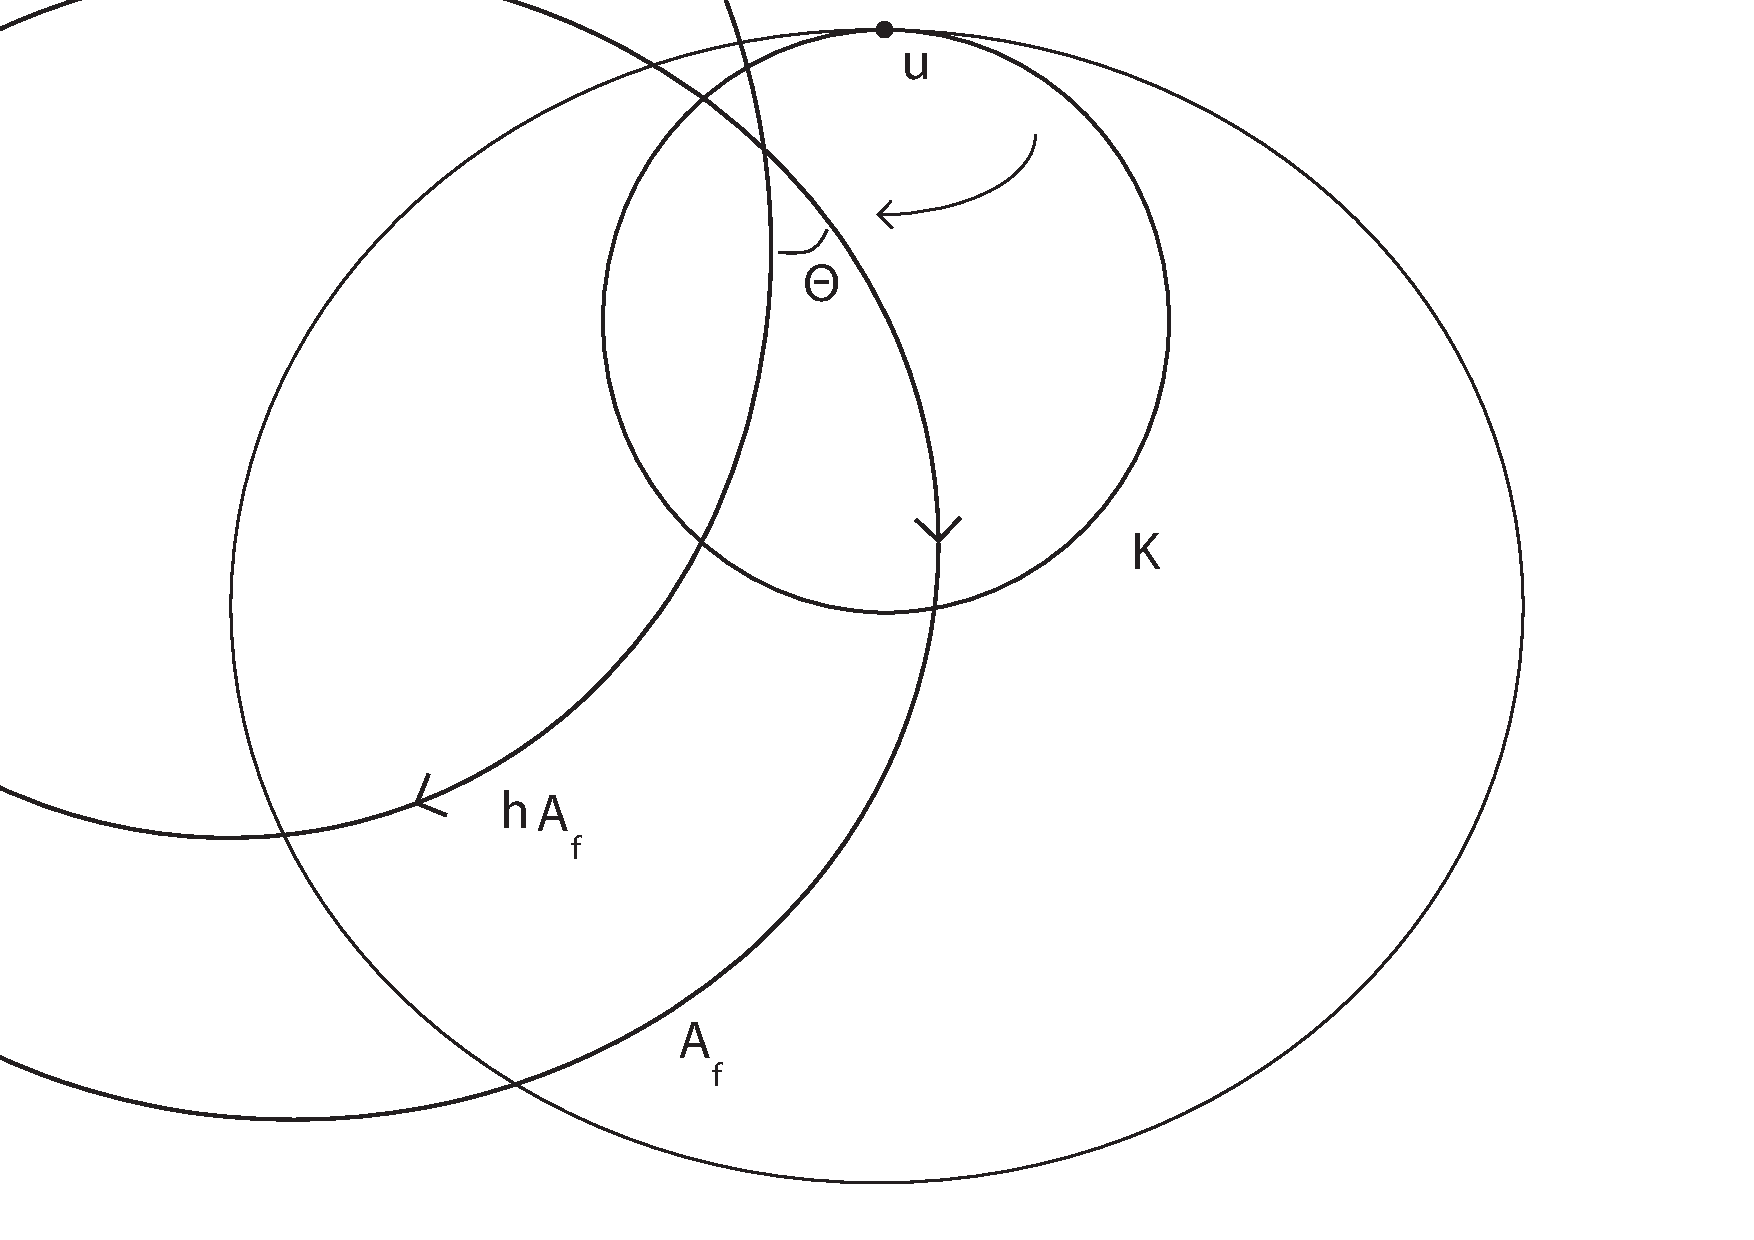
\includegraphics[width=10cm]{lemma5-dibujo3}\\
  \caption{Figura \ref{lemma5-dibujo3}}\label{lemma5-dibujo3}
\end{figure}


Ya que $senh^{2} \frac{1}{2}\lambda_{f}$ es fijo y $sen\phi
\rightarrow 0$ cuando $\phi \rightarrow 0$, y del \textbf{lema} \ref{lema2} se
sigue que $[f,f']$ es el\'iptico. $_{\square}$ \\ \\


\section{El teorema de Nielsen}

Probamos ahora la parte restante del teorema de Nielsen.

Sea $G < PSL(2,\mathbb{R})$ sin puntos invariantes y sin
elementos el\'ipticos. \\

Antes que nada veamos que $G$ no es abeliano. Si los ejes son
divergentes y  $fg = gf$ entonces $fgf^{-1} = g$, pero no es posible
ya que $fgf^{-1}$ fija $fx,fy$ con $x,y $ puntos fijos de $g$, pero
esto implica $fx=y$ y $fy=x$ pero esto implica $f^{2}x=x$, pero
$f^{2}$ fija los mimos puntos que $f$ por tanto no puede fijar los
puntos de $g$. \\

Es an\'alogo si los ejes son paralelos ya que $f$ no puede
intercambiar $x$ y $y$ al mismo tiempo. \\


\begin{figure}[h]
  \centering
  % Requires \usepackage{graphicx}
  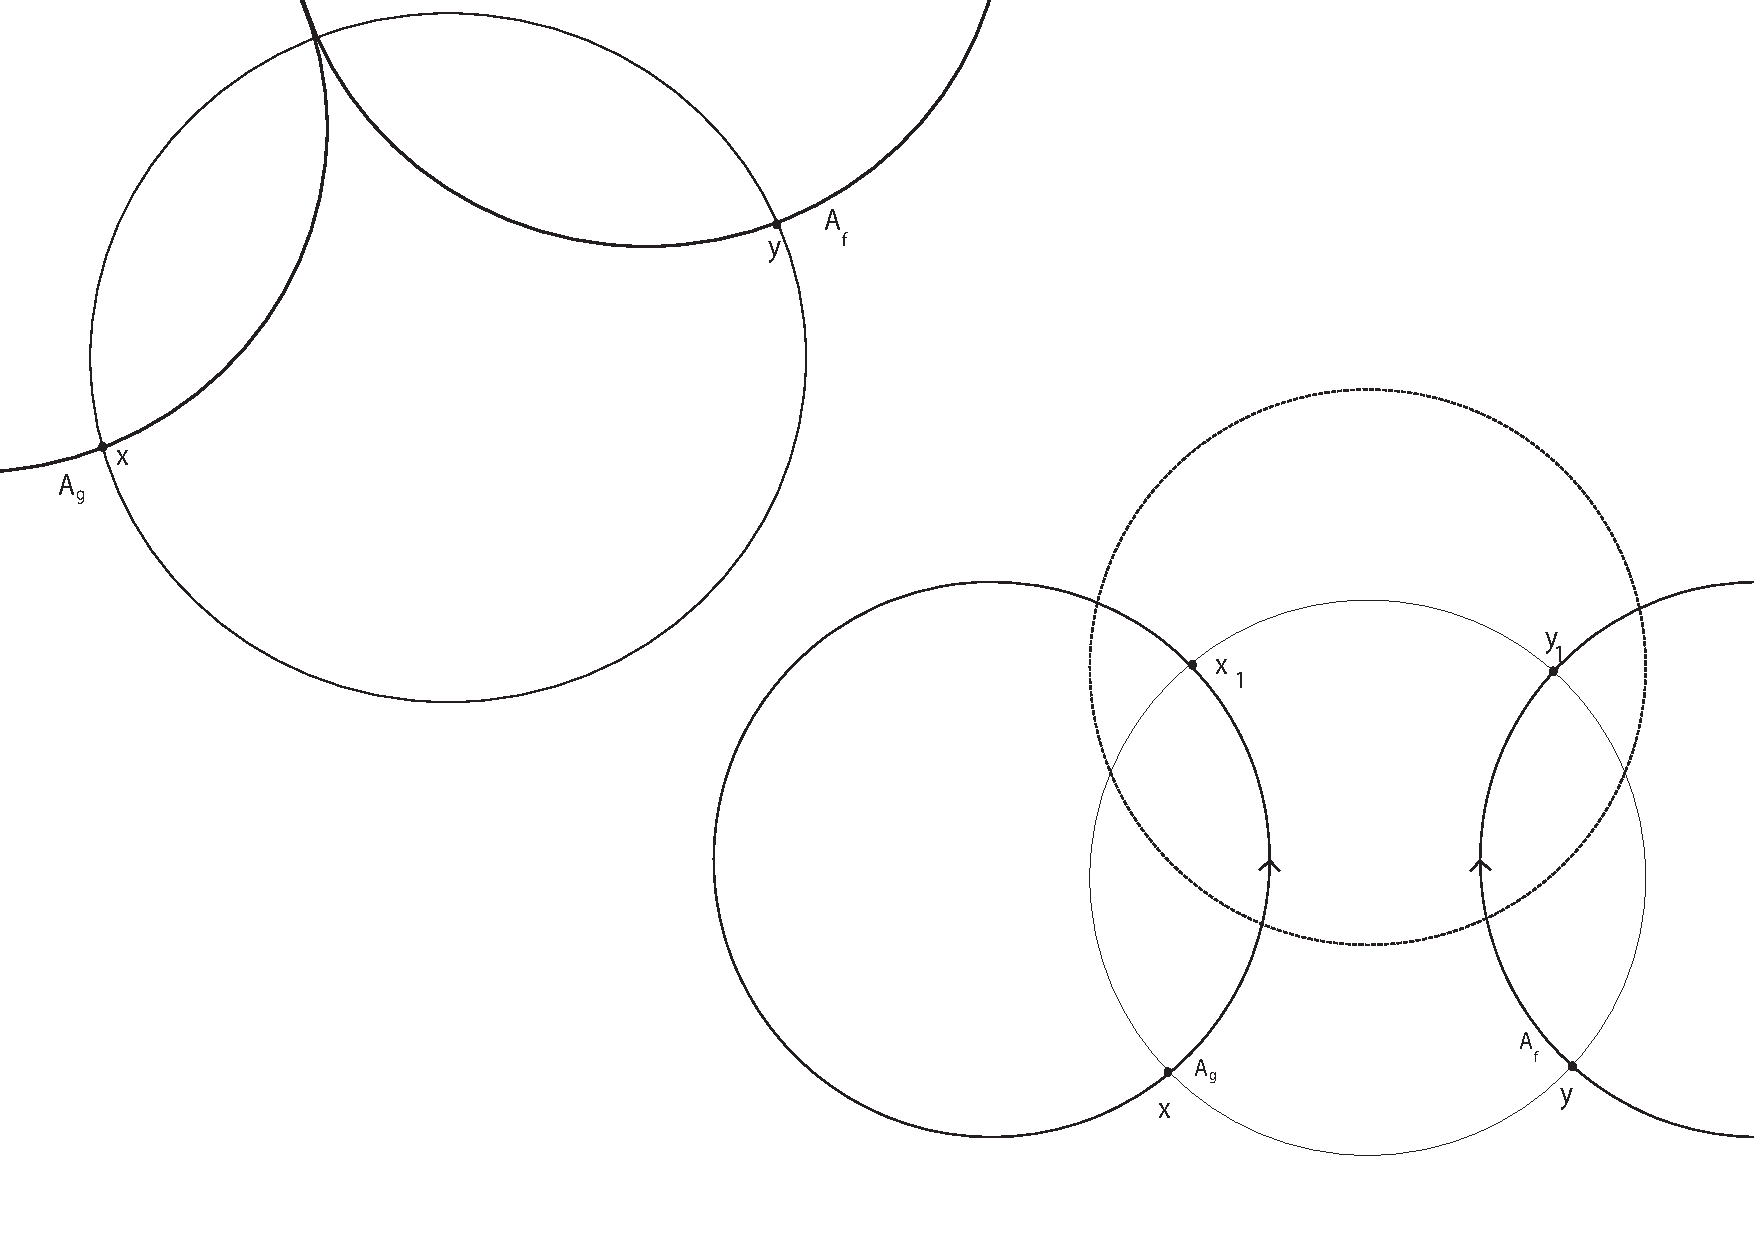
\includegraphics[width=10cm]{lemma6-dibujo-1-2}\\
  \caption{Ejes de f y g paralelos y divergentes}\label{lemma6-dibujo-1-2}
\end{figure}



M\'as a\'un debe haber elementos hiperb\'olicos en $G$, de otro modo
solo tendr\'ia elementos parab\'olicos que por hip\'otesis no
tendrian un punto fijo en com\'un y el lema \ref{lema3} implicar\'ia
una contradicci\'on en este caso. \\

Sea $f$ hiperb\'olico en $G$ y $A_{f} $ su eje y $\lambda_{f}$ la
medida de su desplazamiento, sea $g \in G$ tal que $fg \neq gf$,
entonces $f' = gf^{\pm 1}g^{-1}$ es una hiperb\'olico con el mismo
desplazamiento que $f$ y con eje $gA_{f} \neq A_{f}$ (Por no ser
permutables)(Si $A_{f}=gA_{f} \Rightarrow gfg^{-1}=f$ o
$gfg^{-1}=f^{-1}$. El primer caso es trivial. El segundo caso basta tomar un punto fijo $x$ de $f$ tal que  $g(x)$ no es punto fijo de $f$ (ni de $f^{-1}$) y evaluar en ambos lados de la ecuaci\'on para llegar a una contradicci\'on.) \\

$A_{f},A_{f'}$ no pueden ser paralelas por el lema \ref{lema5}, si
son divergente sea $\delta$ la distancia entre ellas y elijamos $f'$
tal que el exponente de $f$ haga $f$ y $f'$ con desplazamientos
opuestos, por las condiciones impuestas en $G$, $ff'$ no es
el\'iptico y del \ref{lema1} obtenemos

\begin{equation} \label{relacionseno1}
 \  senh \frac{1}{2}
\delta senh \frac{1}{2} \lambda_{f} \geqq 1
\end{equation}

Si $A_{f},A_{f'}$ son concurrentes sea $\phi$ su \'angulo de
intersecci\'on, dado que $[f,f']$ no es una rotaci\'on,  del
\ref{lema2} tenemos

\begin{equation} \label{relacionseno2}
 \ sen \phi senh^{2}\frac{1}{2} \lambda_{f} \geqq 1
\end{equation}

Estas desigualdades se aplican a $g$ fijo y $f$ variando.



\begin{figure}[h]
  \centering
  % Requires \usepackage{graphicx}
  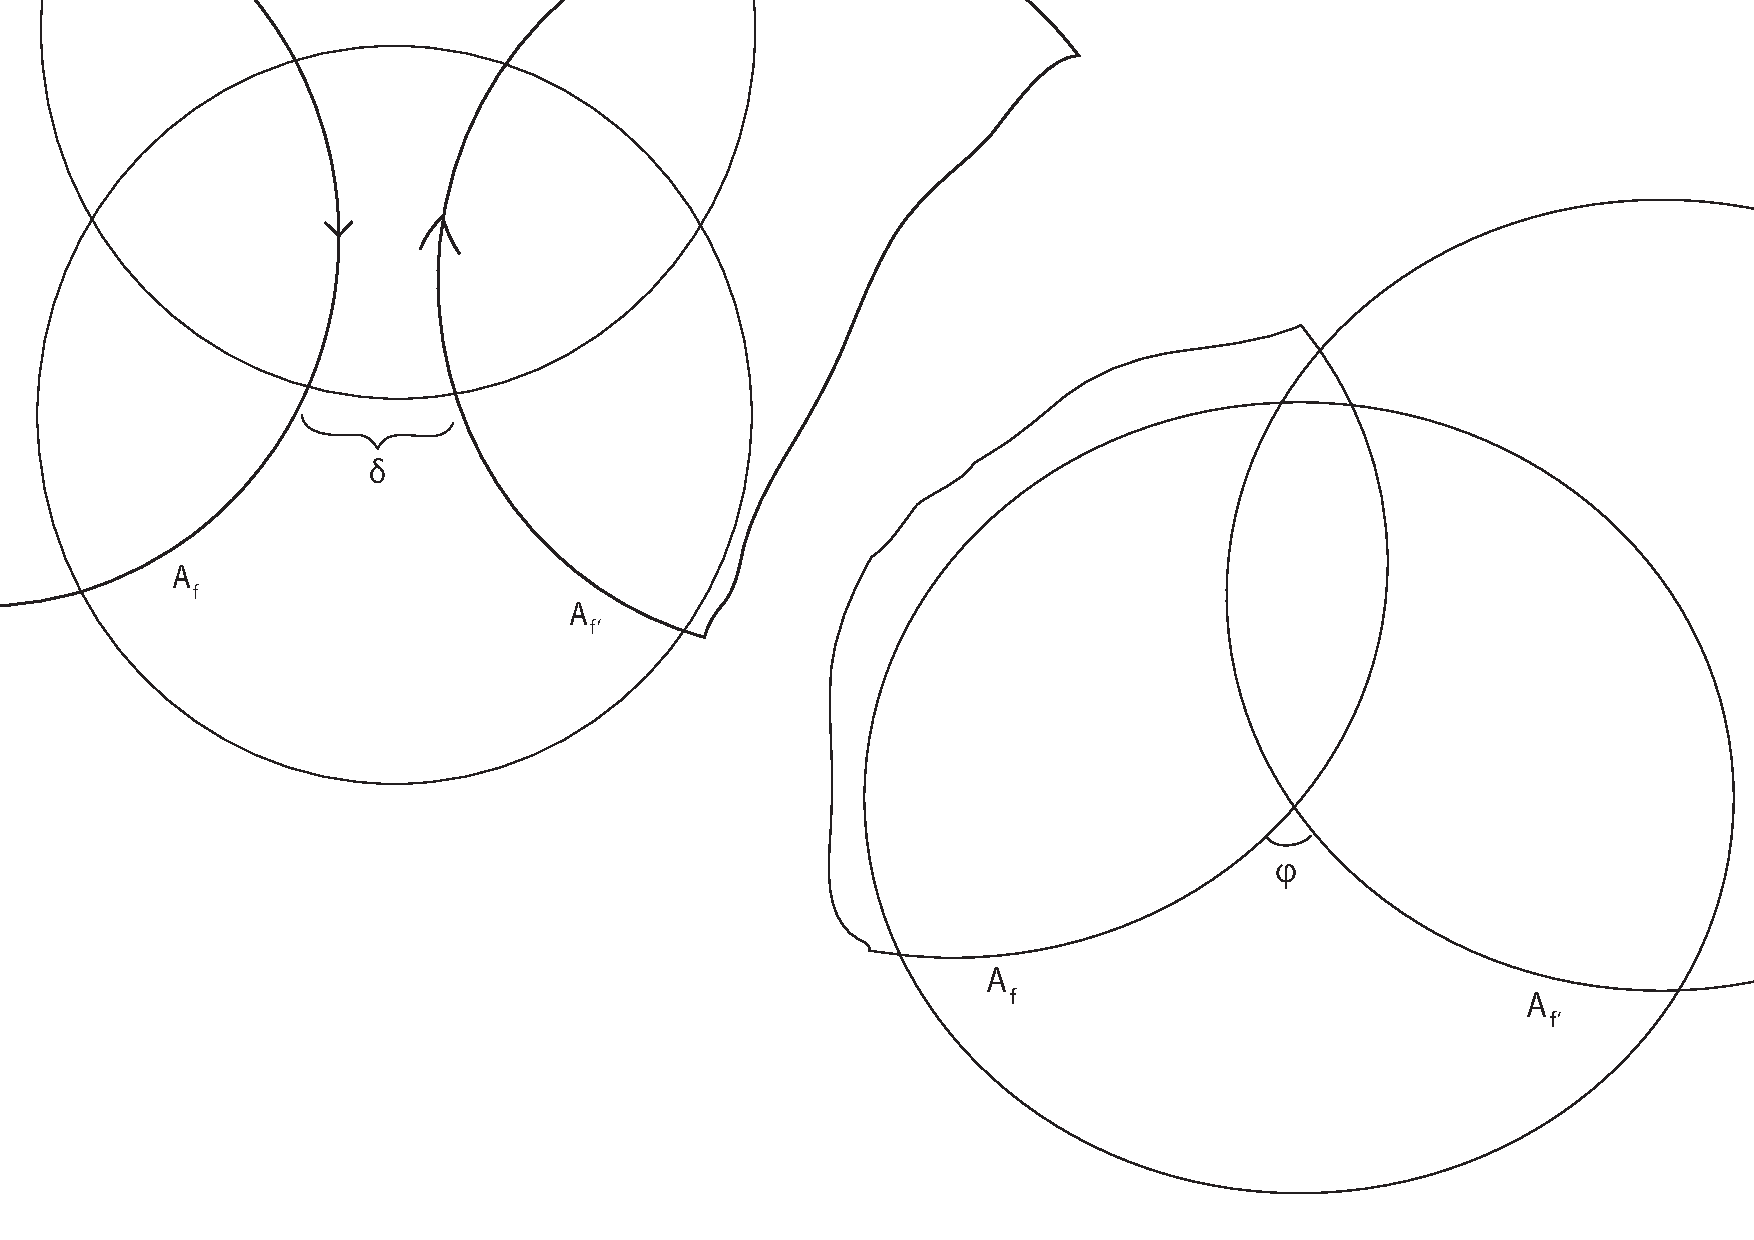
\includegraphics[width=9cm]{lemma6-dibujo-2-4}\\
  \caption{Figura \ref{lemma6-dibujo-2-4}}\label{lemma6-dibujo-2-4}
\end{figure}


Sea $A$ un eje de un elemento hiperb\'olico en $G$, los elementos
hiperb\'olicos que comparten este eje forman un subgrupo abeliano
$S_{A}$ de $G$, sea $g \in G$ un elemento que no tenga como eje a
$A$, es decir que no permuta con los elementos de $S_{A}$, se tiene
que $gA \neq A$. Si $gA$ y $A$ son divergentes digamos que su distancia es $d_{H}(gA,A)= \delta$
si $gA$ y $A$ son concurrentes digamos que se cortan en un \'angulo $\phi$. Dependiendo cual sea el caso aplicaremos \ref{relacionseno1} o \ref{relacionseno2}. \\


Si $f$ varia sobre todos los elementos de $S_{A}$, podemos notar que
todos tienen desplazamiento mayor que un n\'umero positivo distinto
de 1,por las condiciones \ref{relacionseno1} y \ref{relacionseno2} y sabiendo que $senhx \rightarrow 0$ cuando $x \rightarrow 0 $, $\lambda_{f}$ no puede ser arbitrariamente pequeño, m\'as a\'un los desplazamientos no pueden ser arbitrariamente cercanos a la cota, si asi fuera podemos encontrar dos elementos tal que su composici\'on tiene un desplazamiento menor que la cota dada. Entonces $S_{A}$ es discontinuo. Sea $\lambda_{0}$ el desplazamiento mas pequeño de elementos de $S_{A}$ que por lo anterior existe.  \\

Podemos aplicar las mismas desigualdades para $f \in S_{A}$ fijo y
$g $ variando sobre los representantes $g_{1},g_{2},...$ de las
clases de $S_{A} < G$ ($g_{1} \backsim g_{2} \Leftrightarrow
g_{1}S_{A} = g_{2}S_{A} \Leftrightarrow g_{1}g_{2}^{-1} \in S_{A}$).

\begin{rem}
Si $g_{1} \backsim g_{2} \Rightarrow g_{1}A=g_{2}A$ ya que
$g_{1}g_{2}^{-1} = f \in S_{A} \Rightarrow g_{1}g_{2}^{-1}A = fA
\Rightarrow g_{1}g_{2}^{-1}A = A \Rightarrow g_{2}^{-1}A =
g_{1}^{-1}A$
\end{rem}

Los ejes de los elementos hiperb\'olicos $f_{v}=
g_{v}fg_{v}^{-1}$ varian sobre los diferentes ejes de la clase de
equivalencia $GA$ de $A$. \\

Dado que $f_{v}$ tiene el mismo desplazamiento $\lambda_{f}$ que $f$
para todo \'indice $v$, de \ref{relacionseno1} y \ref{relacionseno2} obtenemos que
$senh\frac{1}{2} \delta $ y $sen \phi$ tienen una cota inferior por
lo que $\delta$ y $\phi$ tambi\'en la tienen seg\'un sean
divergentes o concurrentes los ejes $g_{v}A$, esto implica que los
ejes no se acumulan en $D$.  \\


Sea $x \in A$. Todo punto en $Gx$ esta en alg\'un elemento del
conjunto $g_{v}A$. Para un eje dado los puntos $Gx$ que se
encuentran en este eje forman una sucesi\'on de puntos equidistantes
a distancia $\lambda$ (Los puntos en $Gx \cap g_{v}A$ son los puntos
$gx,hx$ tal que $g \backsim h $, luego para $gx,hx \in g_{v}A
\Rightarrow d_{H}(gx,hx)=d_{H}(x,g^{-1}hx), g^{-1}h \in S_{A}
\Rightarrow \lambda_{g^{-1}h} \geqq \lambda_{0}$ (Fig. \ref{lemma6-dibujo6}). \\

\begin{figure}[h]
  \centering
  % Requires \usepackage{graphicx}
  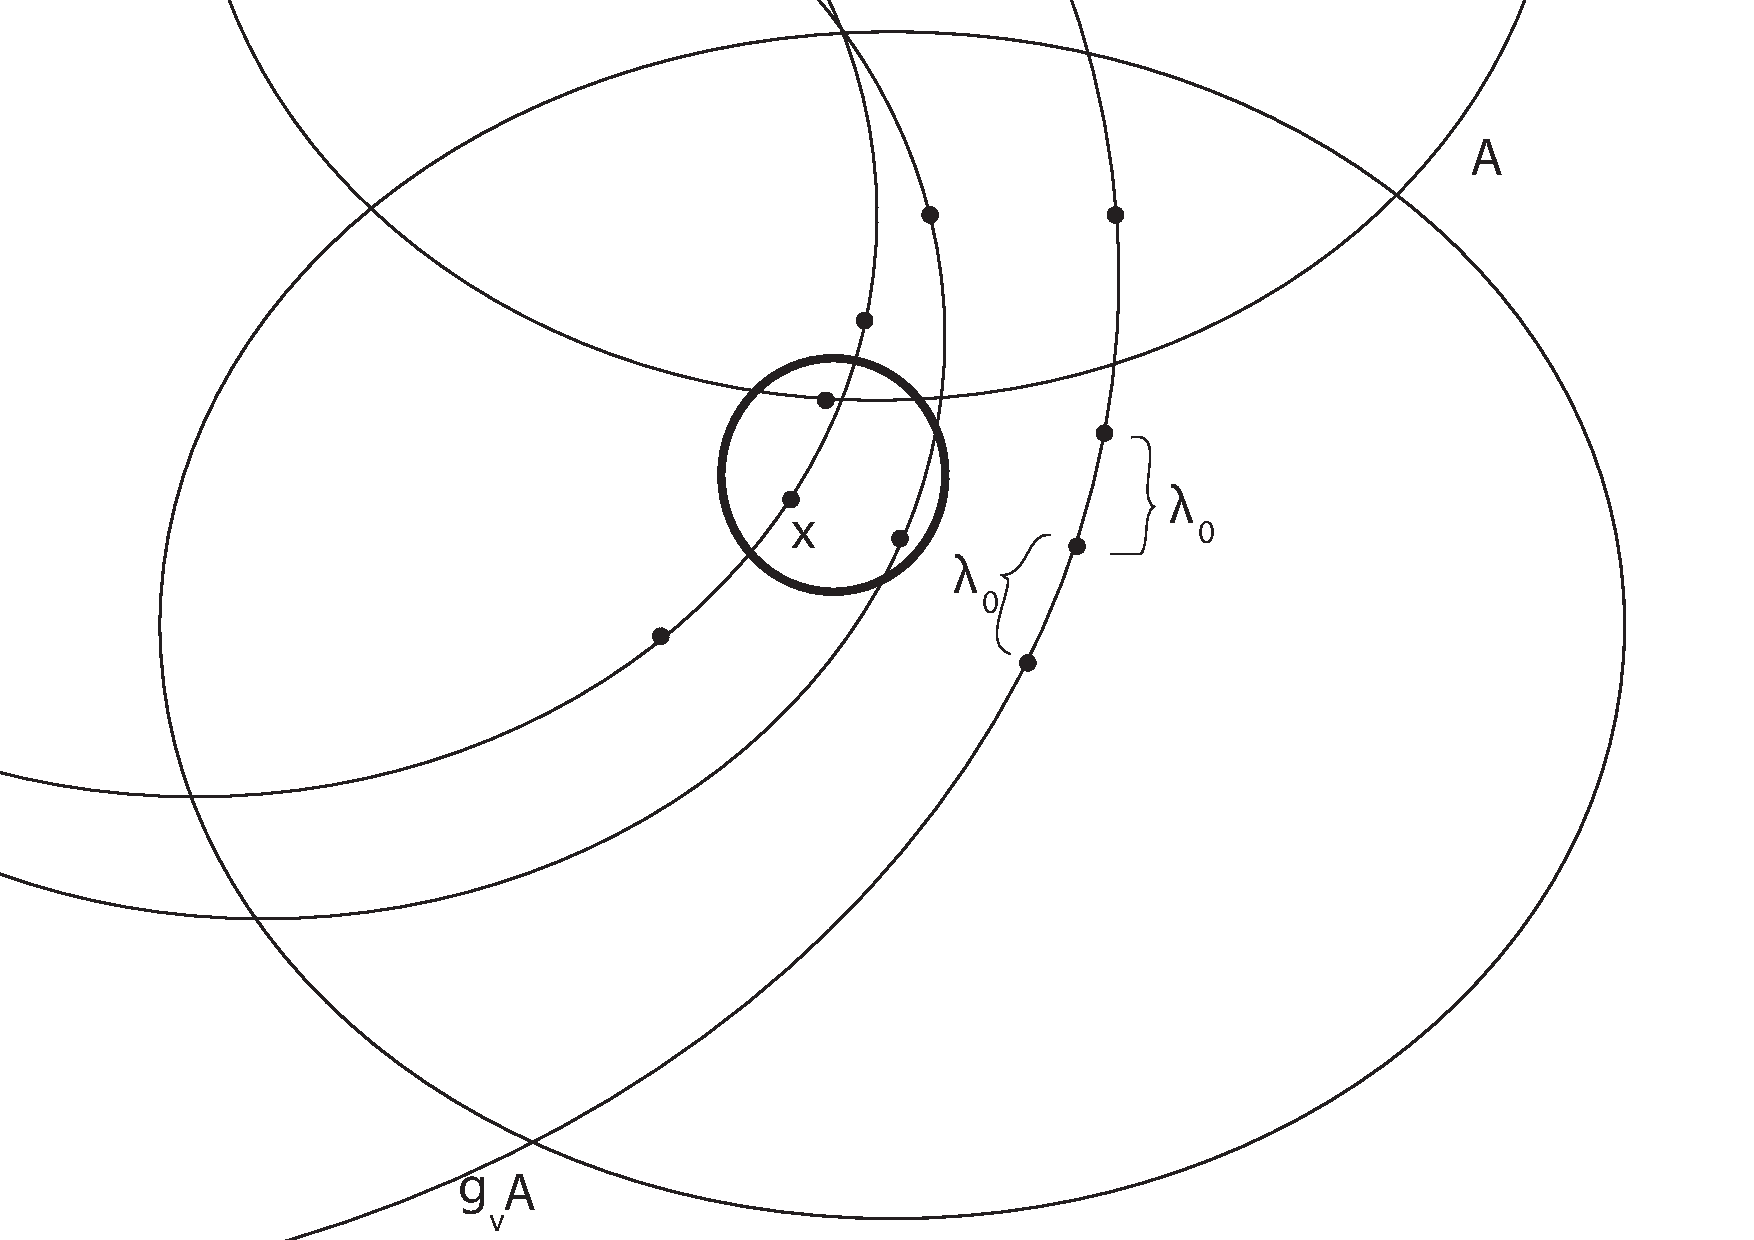
\includegraphics[width=10cm]{lemma6-dibujo6}\\
  \caption{Figura \ref{lemma6-dibujo6}}\label{lemma6-dibujo6}
\end{figure}


El c\'irculo con centro $x$ y radio $\frac{1}{2} \lambda_{0}$
no puede contener mas de un punto de dicha sucesi\'on en su
interior, entonces el n\'umero de puntos en $Gx$ dentro de este
c\'irculo es a lo m'as igual al n\'umero de ejes $g_{v}A$ que cortan
al c\'irculo, este n\'umero es finito ya que los ejes $g_{v}A$ no se
acumulan en $D \  \therefore \ x$ no es punto de acumulaci\'on de
$Gx$. $_{\square}$



\section{Un ejemplo de un grupo discreto}

En el cap\'itulo \ref{cha:grupo schottky} hallamos un grupo de Schottky que es un subgrupo discreto de isometrias hiperb\'olicas, m\'as a\'un sabemos que todos los elementos no triviales del grupo de Schottky son loxodr\'omicos, en nuestro caso hiperb\'olicos, excepto por la identidad, para que podamos validar el teorema de Nielsen en este grupo debemos verificar que se cumplen las condiciones del teorema. Los generadores del grupo de Schottky son hiperb\'olicos por lo cual cada uno tiene una geodesica invariante, podemos usar las matrices del grupo de monodrom\'ia de la ecuaci\'on diferencial hipergeometrica \ref{Matrices_teorema_monodromia_grupo} que son conjugadas a los generadores del grupo de Schottky;

$$  A_{0} =  \begin{pmatrix}
 1& 0\\
 0& \varepsilon (-c)
 \end{pmatrix}  ,\ \ \
A_{1} = P ^{-1}\begin{pmatrix}
 1& 0\\
 0& \varepsilon (c-a-b)
 \end{pmatrix} P
$$


Notamos que $A_{0}$ fija $0,\infty$ y por tanto deja invariante la geod\'esica que los une, podemos ver que $A_{1}$ fija $P^{-1}(0)$ y $P^{-1}(\infty)$ y dado que conocemos $P^{-1}$ podemos calcular ambos valores, por un lado $P^{-1}(0)= \frac{-C}{D}$ por otro lado $P^{-1}(\infty) = \frac{-A}{B}$, y por tanto deja invariante la geod\'esica que une estos dos puntos. Mas abajo probamos que estos dos ejes necesariamente son divergentes.

 En nuestro caso tenemos un grupo de Schottky con dos generadores, sabemos que es libre y tambi\'en es no elemental (\ref{def:elemental}). En \cite{Beardon} encontramos un teorema que dice que para un grupo de transformaciones hiperb\'olicas con las caracteristicas anteriores ser discreto equivale a que act\'ue de manera discontinua seg\'un \ref{def:discontinuo1}, de igual manera en \cite{Beardon} encontramos que \ref{def:discontinuo1} implica \ref{def:discontinuo2}.

 Por otro lado $\Lambda_{\theta}$ posee, salvo la identidad, solo elementos hiperb\'olicos, para aplicar el teorema de Nielsen necesitamos adem\'as que el grupo no tenga ni puntos fijos ni rectas invariantes como mencionamos arriba. En \cite{Beardon} encontramos el siguiente teorema;

\begin{thm}
 Dos transformaciones de Mobius $g,h$ tienen un punto fijo en $\widehat{\mathbb{C}}$ si y solo si $tr[g,h]=2$
\end{thm}

 Haciendo los calculos correspondientes a las matrices asociadas a $\gamma_{1},\gamma_{2}$ obtenemos que; $tr[\gamma_{1},\gamma_{2}] = \frac{2T^{2}(R^{2}-C^{2}) + C^{2}(T^{4} +1)}{T^{2}R^{2}}$, si suponemos que $tr[\gamma_{1},\gamma_{2}]=2$ obtenemos que $C^{2}=0$ o que $T= \pm 1$, ninguno de estos casos es posible debido a las condiciones exigidas, por lo que $tr[\gamma_{1},\gamma_{2}] \neq 2$ es decir $\gamma_{1},\gamma_{2}$  no tienen puntos fijos en $\widehat{\mathbb{C}}$ (en particular no los tiene en $D$) y dado que tienen ejes diferentes, estos necesariamente son divergentes de otro modo su intersecci\'on ser\'ia un punto fijo, por tal motivo no hay rectas invariantes en el grupo generado por estos elementos.Aplicando el teorema de Nielsen se puede concluir que $\Lambda_{\theta}$ es discontinuo en $D$.

Todo lo anterior nos permite afirmar que la familia de  grupos de Schottky hallada en \ref{cha:grupo schottky} son ejemplos en donde podemos verificar el teorema de Nielsen. En la actualidad existen muchos resultados que nos dan la misma informaci\'on que este teorema pero la exposici\'on geom\'etrica de este resultado sigue siendo admirable gracias a su demostraci\'on basada en su mayoria en la geometr\'ia hiperb\'olica pura.


%----------------------------------------------------------------------

	
	
%: ----------------------- conclusion ------------------------
% introduction
%
% this file is called up by thesis.tex
% content in this file will be fed into the main document

%: ----------------------- introduction file header -----------------------
%\begin{savequote}[50mm]
%The logic of validation allows us to move between the two limits of dogmatism and skepticism.
%\qauthor{Paul Ricoeur}
%\end{savequote}


\chapter{El teorema de Nielsen}
\label{cha:El teorema de Nielsen}

% the code below specifies where the figures are stored
%\ifpdf
%    \graphicspath{{4_experiments_and_results/figures/PNG/}{4_experiments_and_results/figures/PDF/}{4_experiments_and_results/figures/}}
%\else
%    \graphicspath{{4_experiments_and_results/figures/EPS/}{4_experiments_and_results/figures/}}
%\fi


%-------------------------------------------------------------------------

%\cite{turing1950computing}

En este cap\'itulo proponemos un teorema sobre la acci\'on discontinua de  grupos de transformaciones que pretendemos aplicar al caso del grupo de monodrom\'ia de la ecuaci\'on hipergeom\'etrica.

Todo en  este cap\'itulo es pensado en el sentido de Poincar\'e y hacemos un breve recordatorio de los conceptos que ocupamos durante el mismo.

Tratamos de dar una caracterizaci\'on de los grupos propiamente discontinuos de transformaciones lineales fraccionales con c\'irculo principal en el sentido de la teor\'ia de automorfismos.
Representamos al plano hiperb\'olico como una regi\'on circular en el plano complejo, este modelo llamado el disco de poincar\'e se divide en dos partes de $\lbrace z | |z| \leq 1 \rbrace$,el interior
le denominamos $D =\lbrace z | |z| <1 \rbrace$ y la frontera la denominamos  $E =\lbrace z| |z| =1  \rbrace$.  Todas las cosecuencias geom\'etricas las entendemos en el sentido no-euclidio. Tambi\'en denotamos por $\mathbb{H} ^{+}$ al modelo hiperb\'olico del semiplano.\\



Llamamos puntos finales a los extremos de una recta situados en
el c\'irculo infinito, e identificamos tres tipos de relaciones entre las rectas, a saber;
concurrentes, paralelas y divergentes. \\

\begin{defn}
Las rectas Paralelas son dos rectas que tienen un punto
final en com\'un.\\
Las rectas Concurrentes son las que se intersectan en $D$.
\\
Las rectas Divergentes son las que no se intersectan en
nig\'un lugar. \\
\end{defn}



\begin{figure}[h]
  \centering
  % Requires \usepackage{graphicx}
  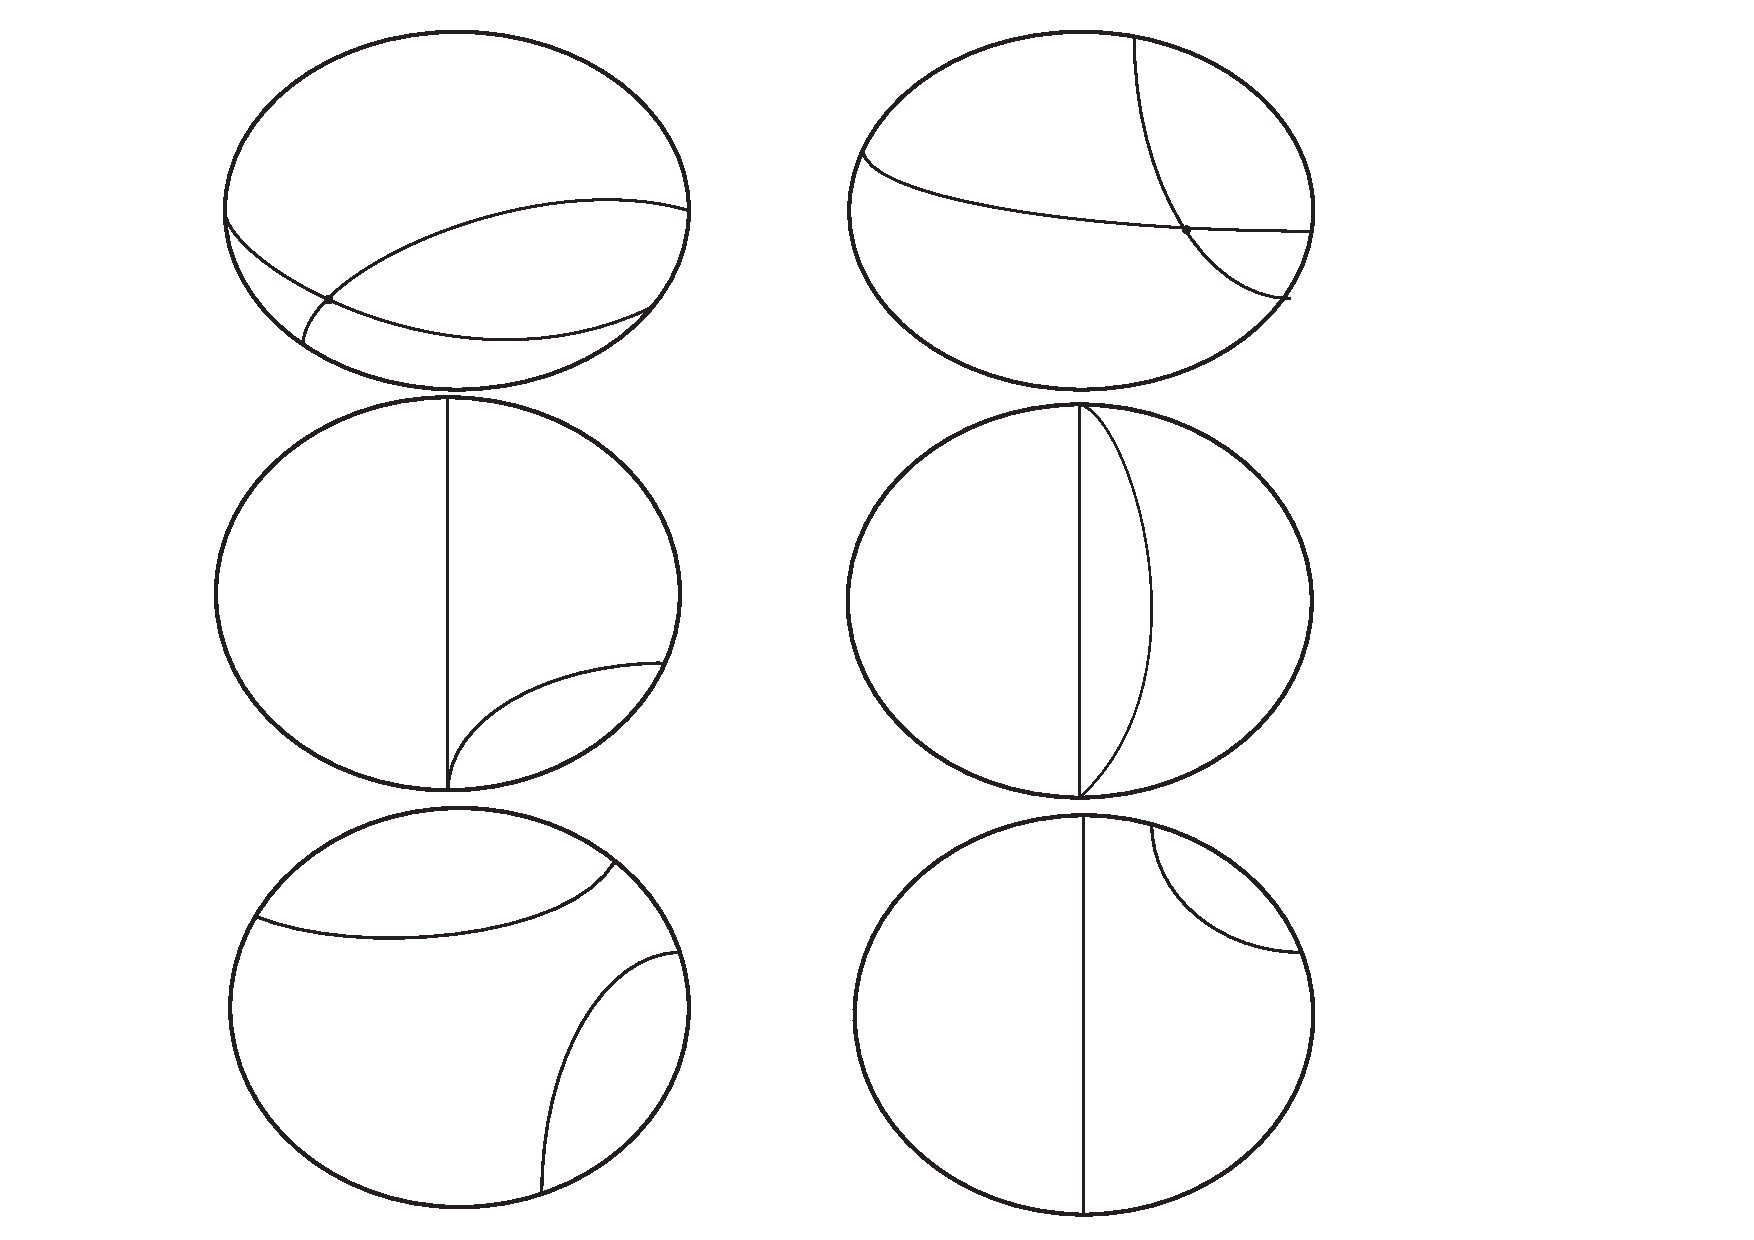
\includegraphics[width=10cm]{rectas-concurrentes-paralelas-divergentes.pdf}\\
  \caption{Rectas hiperb\'olicas concurrentes, paralelas y divergentes respectivamente.}%\label{}
\end{figure}


Los \textbf{Horociclos} son c\'irculos tangentes a alg\'un punto en la
frontera $E$ de $S^{1}$.Es importante dejar en claro que los Horociclos no son geod\'esicas. \\


Los \textbf{hiperciclos} se forman por una recta $\emph{L}$ y un
punto $\textbf{P}$ fuera de ella, el hiperciclo es  el lugar geom\'etrico
de todos los puntos a distancia $d_{H}(\textbf{P},\emph{L})$,  de
$\emph{L}$ y del mismo lado de $P$.  $d_{H}$ es la distancia hiperb\'olica.
 De igual manera los hiperciclos no son geod\'esicas. \\


Dividiremos las transformaciones isom\'etricas en dos grupos, las
que preservan la orientaci\'on y las que no. En el grupo de las que
preservan la orientaci\'ion distinguimos tres tipos distintos de
transformaciones; \\

\begin{defn}
Las transformaciones \textbf{parab\'olicas} tienen un punto fijo en
$E$ y dado un horociclo $K$ tangente en dicho punto fijo a $E$, esta
transformaci\'on tiene un desplazamiento fijo en $K$.


Las tranformaciones \textbf{el\'ipticas} tienen un punto fijo en $D$
y un \'angulo fijo $\phi$ de rotaci\'on en torno al punto fijo.


Las transformaciones \textbf{hiperb\'olicas} tienen dos puntos fijos
en $E$ y una recta invariante, la recta que pasa por dichos puntos
fijos la llamamos eje de la transformaci\'on.


\begin{figure}[h]
  \centering
  % Requires \usepackage{graphicx}
  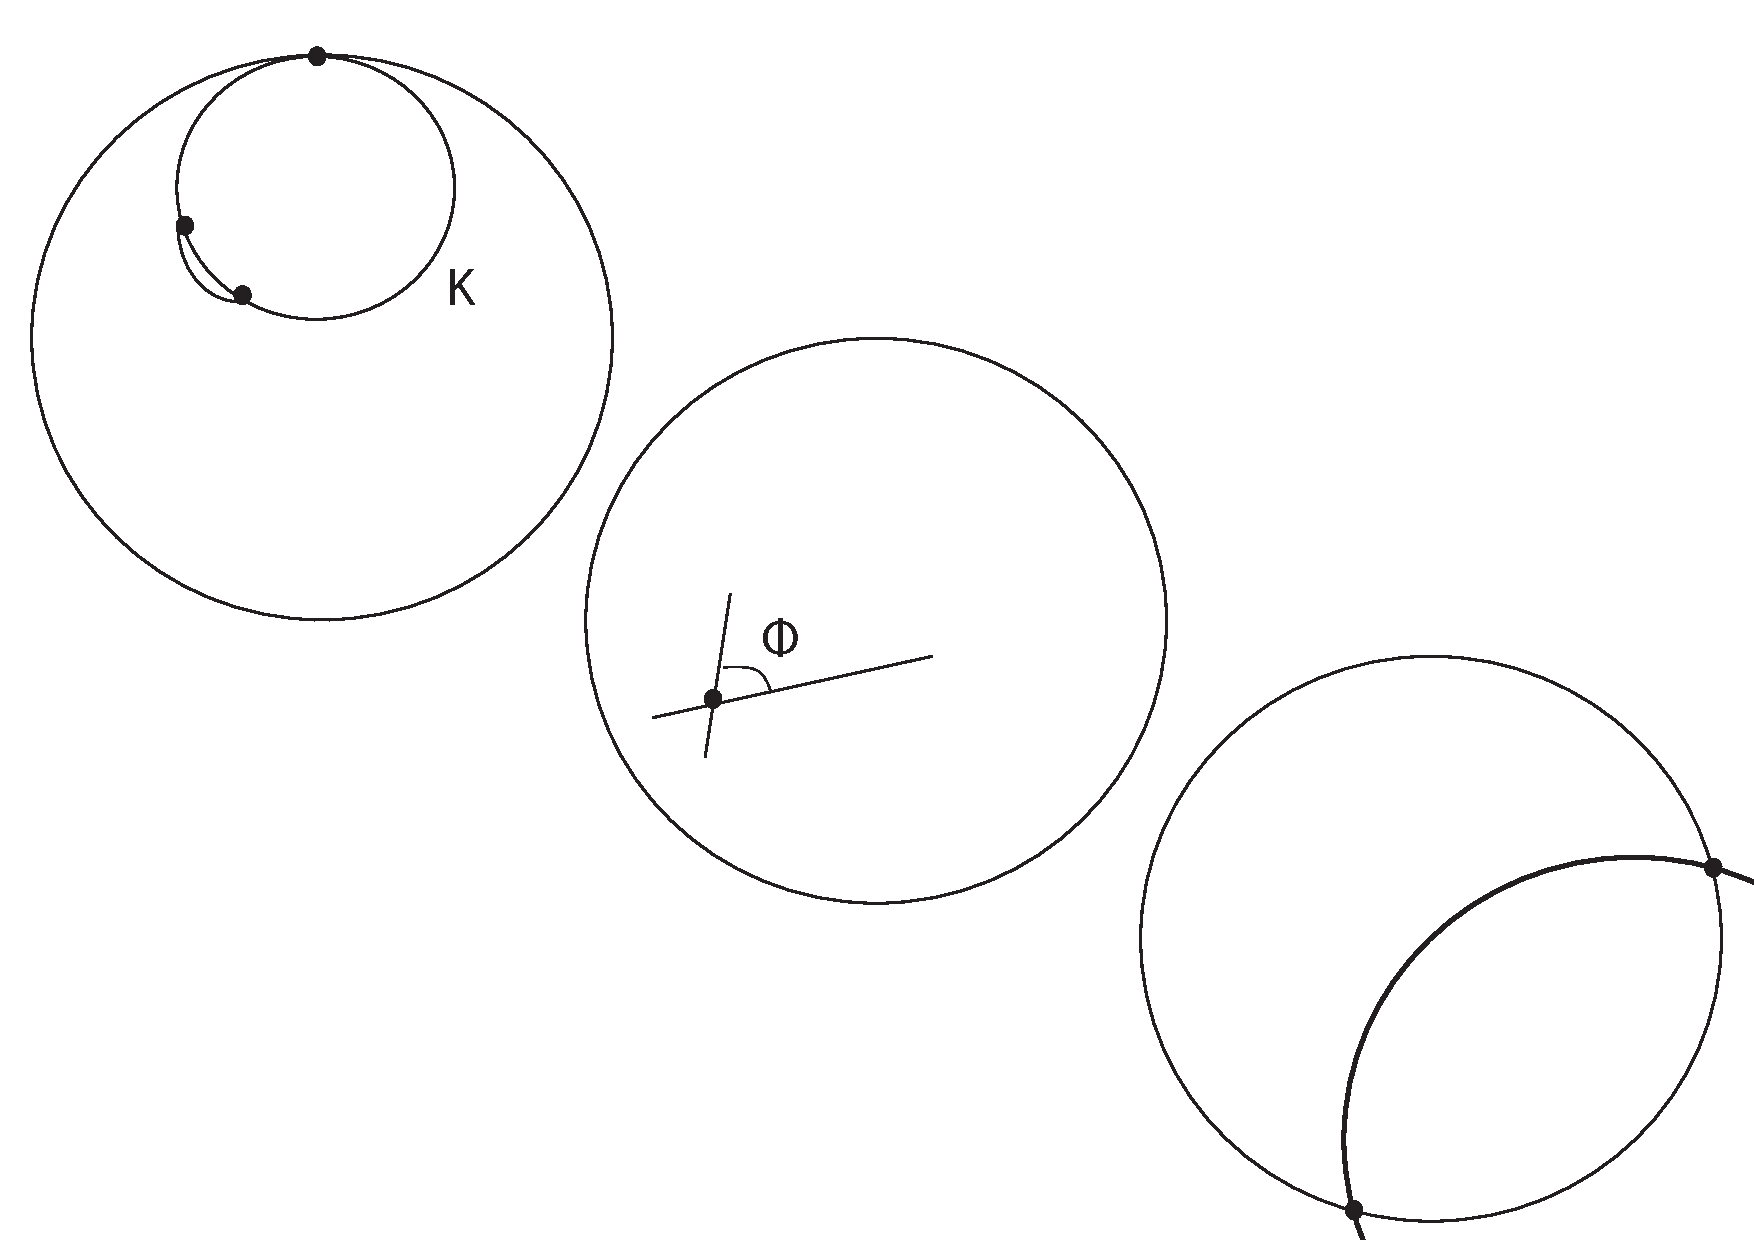
\includegraphics[width=8cm]{definicion40.pdf}\\
  \caption{Representaci\'on de los puntos importantes en las transformaciones hperb\'olicas}\label{definicion40}
\end{figure}


\end{defn}

Si $G$ es un grupo de transformaciones isom\'etricas, un punto
invariante para $G$ es un punto fijo bajo todos los elementos de $G$, de
una manera similar pensamos en una recta invariante. \\

Un par de conjuntos de puntos $M$ y $M'$ en $D + E$ son equivalentes respecto a
$G$ si existe $f \in G$ tal que $M = fM'$. El total de conjuntos
equivalentes de $M$ se denota como la familia $GM$ llamada clase de
equivalencia de $M$, en esta familia si $f_{1},f_{2} \in G  $ y
$f_{1} \neq f_{2 }$ entonces $f_{1}M \neq f_{2}M$ sin importar que
como conjunto sean iguales. \\

\begin{defn}
Decimos que $G$ es discontinuo en un punto $x \in D$,si $x$ no es un
punto de acumulaci\'on de la clase $Gx$, si esto sucede $Gx$ no
tiene puntos de acumulaci\'on en $D$
\end{defn}

\begin{prop}
Si $G$ es discontinuo en $x$, $G$ no tiene puntos de acumulaci\'on en $D$.
\end{prop}

\textit{Prueba}:

Supongamos que $G$ es discontinuo en $x$, existe $m$ tal que $\forall \ i,j, \  d_{H}(g_{i}x,g_{j}x) > m$, de otro modo $x$ ser\'ia un punto de acumulaci\'on de $Gx$. Sea $y$ un punto arbitrario de $D$ y sea $U_{r}$ una vecindad de $y$ de radio $r < m$, entonces a lo m\'as hay un punto $gx$ de $Gx$ en $U_{r}$, si tomamos $V_{r'}$ vecindad de $y$ con $r' < d_{H}(gx,y)$, esa vecindad no contiene puntos de $Gx$. $_{\square}$

Esto implica que si $G$  es discontinuo en un punto de  $D$ entonces es discontinuo en todo
$D$.\\

Las \'unicas isometr\'ias de $\mathbb{H}^{+} $ que preservan la orientaci\'on
son las de $PSL(2,\mathbb{R})$, las transformaciones mencionadas con
anterioridad se encuentran en este grupo. Si $f \in PSL(2,\mathbb{R})$ y $g$  otra transformaci\'on  entonces $gfg^{-1}$ es de la misma clase que $f$.\\

Llamaremos \textbf{reversiones} a las transformaciones que invierten
la orientaci\'on, las reversiones son las \textbf{reflexiones}
respecto a una recta, y las reflexiones compuestas con elementos
hiperb\'olicos a las que llamamos \textbf{h-reflexiones}. \\


La reflexi\'on respecto a una recta hiperb\'olica es la reflexi\'on
respecto a una circunferencia euclidiana. \\


\begin{thm} \label{Teorema-nielsen} [Teorema de Nielsen]
Una condici\'on necesaria y suficiente para que un grupo de
transformaciones isom\'etricas en el plano hiperb\'olico sin puntos
ni lineas invariantes sea discontinuo en $D $ es que los puntos
fijos de los elementos el\'ipticos del grupo, si los hay, no se
acumulen en $D$

\end{thm}

La condici\'on de que no tenga puntos ni rectas invariantes es
necesaria, como podemos ver en los siguientes casos.

\begin{enumerate}
\item Si $G$ es un grupo de elementos parab\'olicos con un mismo punto
fijo al infinito.
\item Si $G$ es un grupo de elementos hiperb\'olicos con una recta fija
dada.
\end{enumerate}

Ninguno de los anteriores contiene elementos el\'ipticos sin embargo
ninguno es discontinuo en $D$.\\

Si $G$ contiene reversiones  y $H$ es un subgrupo de $G$ y adem\'as $H
\subseteq PSL(2,\mathbb{R})$ se tiene que $H$  es normal y de \'indice 2. Es normal ya que si $f \in H$
para cualquier elemento $g \in G$ se tiene que $gfg^{-1}$ es del
mismo tipo que $f$ por lo que $gfg^{1} \in H$, es de \'indice 2,
para ver esto basta probar que si $f,g \in G - H$ entonces $f \cong
g$ equivalentemente que $fg^{-1} \in H$, dado que $f , g$ revierten
orientaci\'on  se tiene que $fg^{-1}$ conserva la orientaci\'on y
por lo tanto esta en
$H$. \\

Una clase de equivalencia $Gx$ es la suma de las clases $Hx$ y $Hgx$
con $g$ una reversi\'on en $G$ ($H \cup Hg = G \Rightarrow Hx \cup
Hgx = Gx $ ), por lo que se concluye que $G$ y $H$
son ambos discontinuos en $D$ o ambos no lo son. En otras palabras $H$ es discontinuo en $D$ si y solo si $G$ lo es.


\begin{prop} Si $G$ no tiene rectas ni puntos invariantes tampoco los
tiene $H$.
\end{prop}

\textit{Prueba}:

 Supongamos que $H$ deja invariantes un punto en $D +E$,
pero ning\'un otro punto (y por tanto ninguna recta), como $G$ no
deja puntos invariantes, existe $g \in G $ tal que $gc \neq c$ luego
el subgrupo $gHg^{-1}$ deja invariante $gc$ pero ningun otro punto en
$D+E$ pero como $H \vartriangleleft G$ se tiene que  $gHg^{-1}=H$ y
como $gc \neq c $ implica que $H$ fija $c$ y $gc$ lo cual es una
contradicci\'on, concluimos que $H$ no deja puntos invariantes. Un
razonamiento an\'alogo nos enseña que $H$ no deja rectas invariantes. $_{\square}$ \\


Desde ahora  $G$ denotar\'a un subgrupo de $PSL(2,\mathbb{R})$ sin
puntos ni rectas invariantes. \\

Ahora probamos el \textbf{Teorema} \ref{Teorema-nielsen} para el caso cuando el grupo tiene elementos el\'ipticos.

\textit{Prueba}:

Primero probaremos que si los puntos fijos de los elementos el\'ipticos se
acumulan $\Rightarrow$ $G$ no es discontinuo en $D$ \\

Supongamos que los puntos fijos de los elementos el\'ipticos se
acumulan en $D$ (tiene un punto de acumulaci\'on en $D$), es posible
encontrar una sucesi\'on de puntos fijos que convergen al punto de
acumulaci\'on digamos $x$ (por ser espacio m\'etrico) y sean estos $y_{1},y_{2},...$ y
$f_{1},f_{2},...$ los respectivos elementos el\'ipticos. Por un lado
$d_{H}(y_{i},x) \leq \epsilon $ para $i$ adecuada, considerando $\lbrace
f_{i}x\rbrace$ podemos notar que

$$ d_{H}(f_{i}x,x) \leq d_{H}(f_{i}x,y_{i}) + d_{H}(y_{i},x) = 2d_{H}(y_{i},x)$$

Lo anterior debido a que $f_{i}$ fija $y_{i}$ y que es una
isometr\'ia. Luego entonces $f_{i}x \rightarrow x$, es decir $Gx$ se
acumula en $x$  por tanto $G$ no es discontinuo en $x$ y por lo
tanto no lo es en $D$.\\

Si los puntos fijos de los elementos el\'ipticos no se acumulan en $D$
$\Rightarrow$ $G$ es discontinuo en $D$.\\

Sea $c$ un punto fijo de alg\'un elemento el\'iptico en $G$. Basta notar que $Gc$ contiene solo puntos fijos de elementos el\'ipticos de $G$, observando que para $g(c) \in Gc$ el elemento $gfg^{-1} \in G$ lo deja fijo si $f $ es un elemento el\'iptico que fija $c$, luego $c$ no es un punto de acumulaci\'on de $Gc$ ya que los puntos fijos de elementos el\'ipticos no se acumulan, entonces $G$ es discontinuo en $c$ y por lo tanto $G$ es disontinuo en $D$.

%Elegimos un elemento el\'iptico $f $ y sea $c$ su punto fijo, como
%$G$ no tiene puntos invariantes existe $g \in G $ tal que $g(c) \neq
%c$ y adem\'as $g(c)$ es punto fijo de $gfg^{-1} $ que es de igual
%manera un elemento el\'iptico. Sea $G(c)$ el subgrupo de $G$ de
%elementos el\'ipticos con punto fijo $c$ entonces la cardinalidad $\sharp G(c) <
%\infty$, para ver esto notemos 2 cosas;

%\begin{enumerate}
%\item $hg(c)$ es punto fijo de alg\'un elemento el\'iptico en $G$ a
%saber $hgfg^{-1}h^{-1}, \forall h \in G(c)$
%\item $d_{H}(g(c),c)=d_{H}(hg(c),h(c))=d_{H}(hg(c),c)$
%\end{enumerate}

%Esto implica que el conjunto $G(c)g(c)$ esta contenido en una
%circunferencia con centro $c$, si $G(c)g(c)$ es infinito y dado que la
%circunferencia es compacta $G(c)g(c)$ tendria un punto de
%acumulaci\'on en dicha circunferencia lo cual contradice nuestra
%hip\'otesis, entonces necesariamente  $\sharp G(c) < \infty$, luego
%se tiene que $Gc$ se compone de puntos fijos de elementos
%el\'ipticos (gc es punto fijo de $gfg^{-1}$ ) en $G$. \\

%Si $gc \in Gc$ se tiene  $\sharp G(c) = \sharp G(gc)$ ya que se
%tiene la biyecci\'on $f \mapsto gfg^{-1}$ con inversa $h \mapsto g^{-1}hg$.



\section{El lema de los elementos hiperb\'olicos con ejes divergentes}

\begin{lem} \label{lema1}
Sean f y g elementos hiperb\'olicos cuyos ejes son divergentes y
cuyos desplazamientos $\lambda$ miden lo mismo pero tienen sentidos
opuestos, y sea $\delta$ la distancia entre sus ejes, entonces $fg$
es el\'iptico, parab\'olico o hiperb\'olico dependiendo de
$$senh \frac{1}{2} \delta senh \frac{1}{2} \lambda    \left \{ \begin{matrix} > 1 & \mbox{ }\mbox{ }
\\ =1 & \mbox{ }\mbox{ } \\ <1 \mbox{} {}\end{matrix}\right. $$
\end{lem}

\textit{Prueba}:

Como los ejes son divergentes existe una normal com\'un a ambos y a
esta recta le llamamos $s'$, denotemos a los ejes de $f$ y $g$ como
$A_{f}$ y $A_{g}$ respectivamente, entonces la normal que
mencionamos antes corta a $A_{f}$ en $a$ y a $A_{g}$ en $a'$ (Fig. \ref{lemma1-dem1}) y
elegimos $b,b'$ en $A_{f}$ y $A_{g}$ respectivamente  de tal manera
que $d_{H}(a,b)=d_{H}(a',b')= \frac{1}{2} \lambda$ y adem\'as en la
direcci\'on que se desplaza $f$. Sean $s,s''$ las rectas normales a
$A_{f},A_{g}$ en $b, b'$ y por abuso de notaci\'on las reflexiones
respecto a estas rectas y $s'$ se denotaran de la misma manera. (Fig. \ref{lemma1-dibujo4}) \\ \\

Queremos ver que tenemos la relaci\'on $f=ss'$, es claro que $ss'$
preserva $A_{f}$ ya que $s'$ lo preserva y $s$ tambi\'en por ser
normal a este eje (las circunferencias ortogonales son invariantes bajo inversiones
entre  ellas), para ver que tiene el mismo sentido que $f$
basta ver hacia donde desplaza un punto y es f\'acil si tomamos $a$ que
queda fijo bajo $s'$ y bajo $s$ se desplaza en la misma direcci\'on
que $f$, por \'ultimo hay que verificar que $d_{H}(x,ss'x) = \lambda
$ pero como $ss'$ preserva la orientaci\'on y tiene dos puntos fijos
(los puntos finales del eje fijo) necesariamente tiene que ser un
elemento hiperb\'olico y para saber cuanto mide su desplazamiento de
nuevo basta verificarlo para un punto en la recta fija y tomando 
de nuevo $a$ notamos que $d_{H}(a,ss'a)= d_{H}(a,sa)= \lambda$, en
conclusi\'on $f=ss'$ y un proceso an\'alogo nos permite probar que
$g=s's''$. \\

\begin{figure}[h]
  \centering
  % Requires \usepackage{graphicx}
  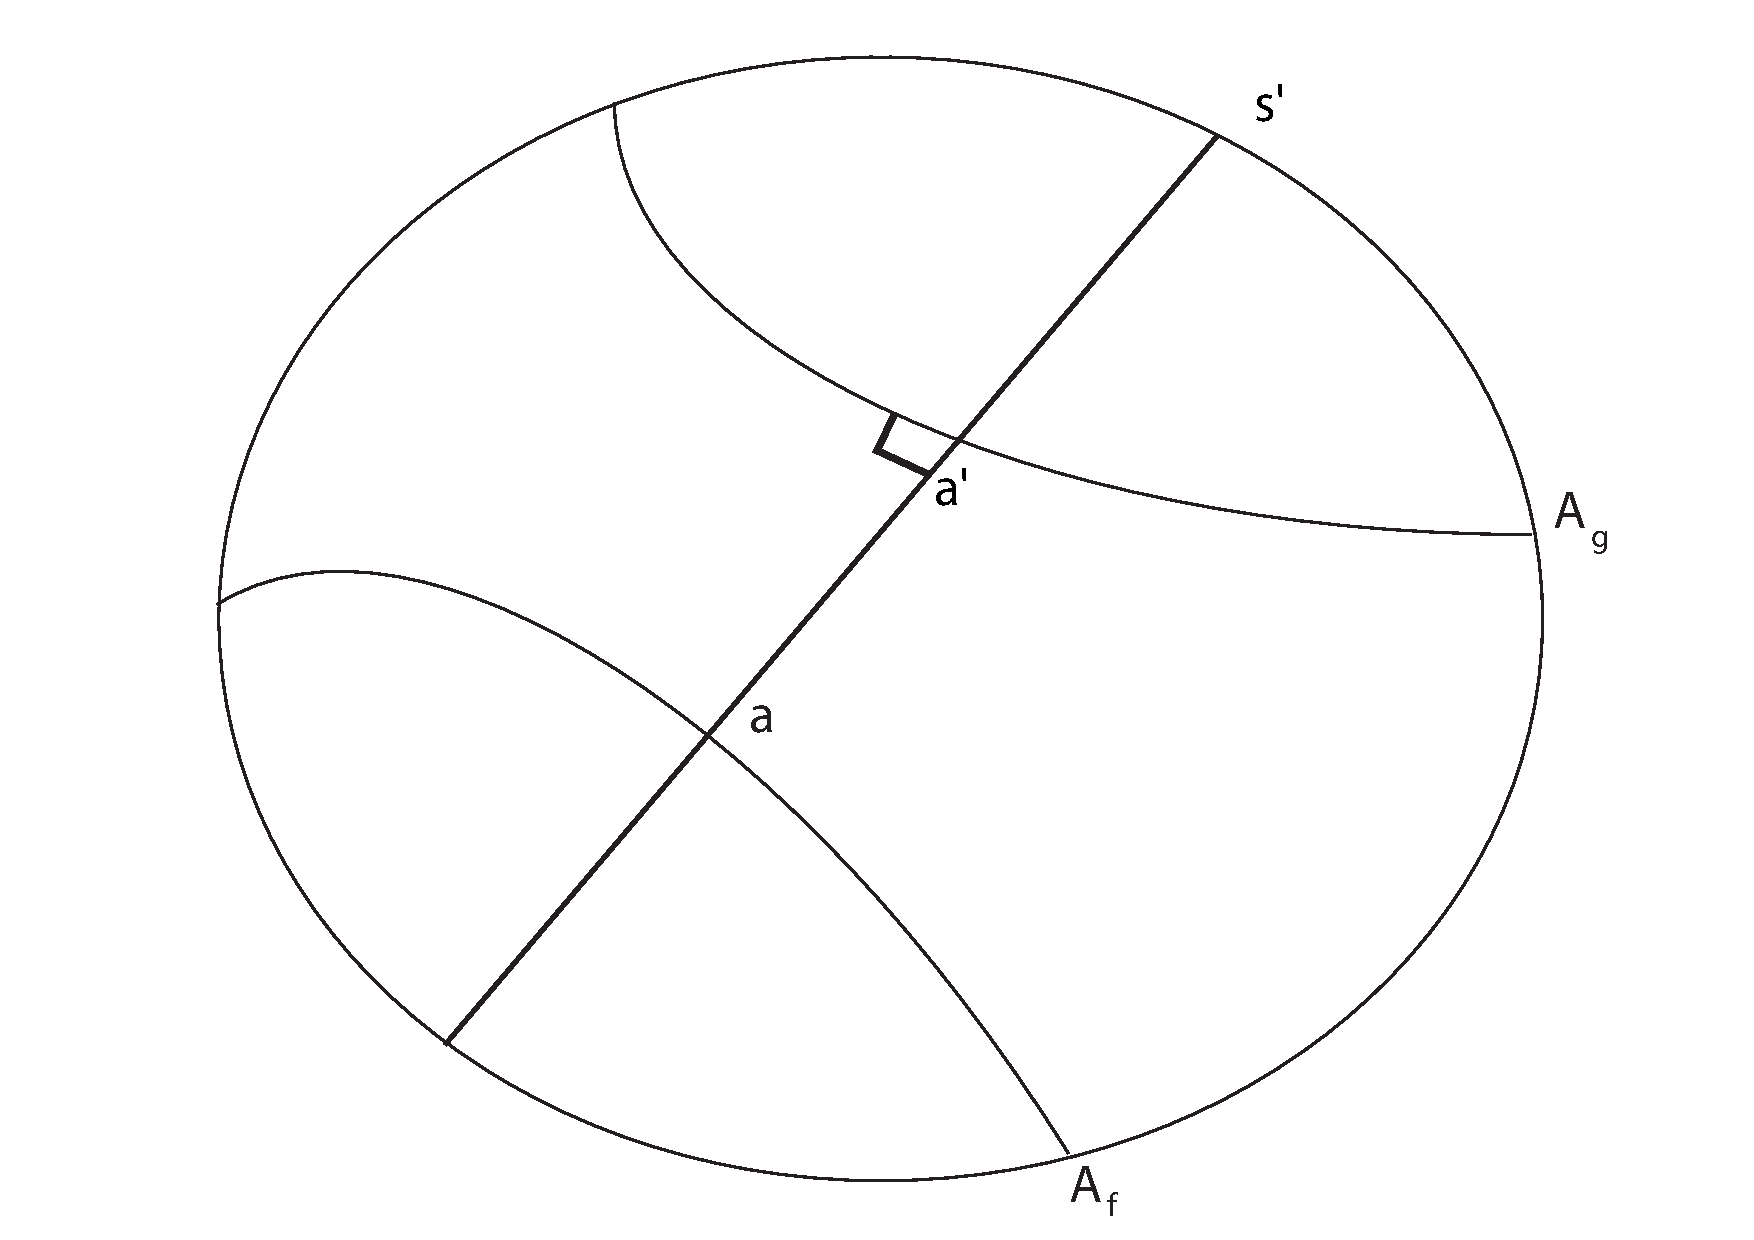
\includegraphics[width=10cm]{lemma1-dem1.pdf}\\
  \caption{Figura \ref{lemma1-dem1} }\label{lemma1-dem1}
\end{figure}


Queremos saber ahora que tipo de transformaci\'on es $fg$, por lo
anterior tenemos que $fg= ss's's'' = ss''$, ahora todo depende de la
posici\'on de los ejes de $f$ y $g$. \\ \\


\textbf{ Caso 1.}[las rectas se intersectan el alg\'un punto de
$D+E$] \\


Sea $m$ el punto medio del segmento $aa'$, la normal a $s'$ que
pasa por $m$ bisecta el \'angulo que forman los ejes en el punto de
intersecci\'on $p$ (\ref{lemma1-dibujo4}), para
ver esto reflejamos las rectas $l$ y $\sigma$ respecto de $l$
obtenemos $l$ y $s''$, como la reflexi\'on es conforme el \'angulo
entre $l$ y $s''$ es el mismo que el \'angulo entre $l$ y $s$. Es
claro que el punto de intersecci\'on $p$ sera el punto fijo de la
transformaci\'on, sea $\frac{1}{2} \phi_{fg}$ el \'angulo entre $s$
y $s'$ (la inversi\'on respecto a dos circunferencias es un elemento el\'iptico con \'angulo el doble del \'angulo de
esta interseccion). \\

\begin{figure}[h]
  \centering
  % Requires \usepackage{graphicx}
  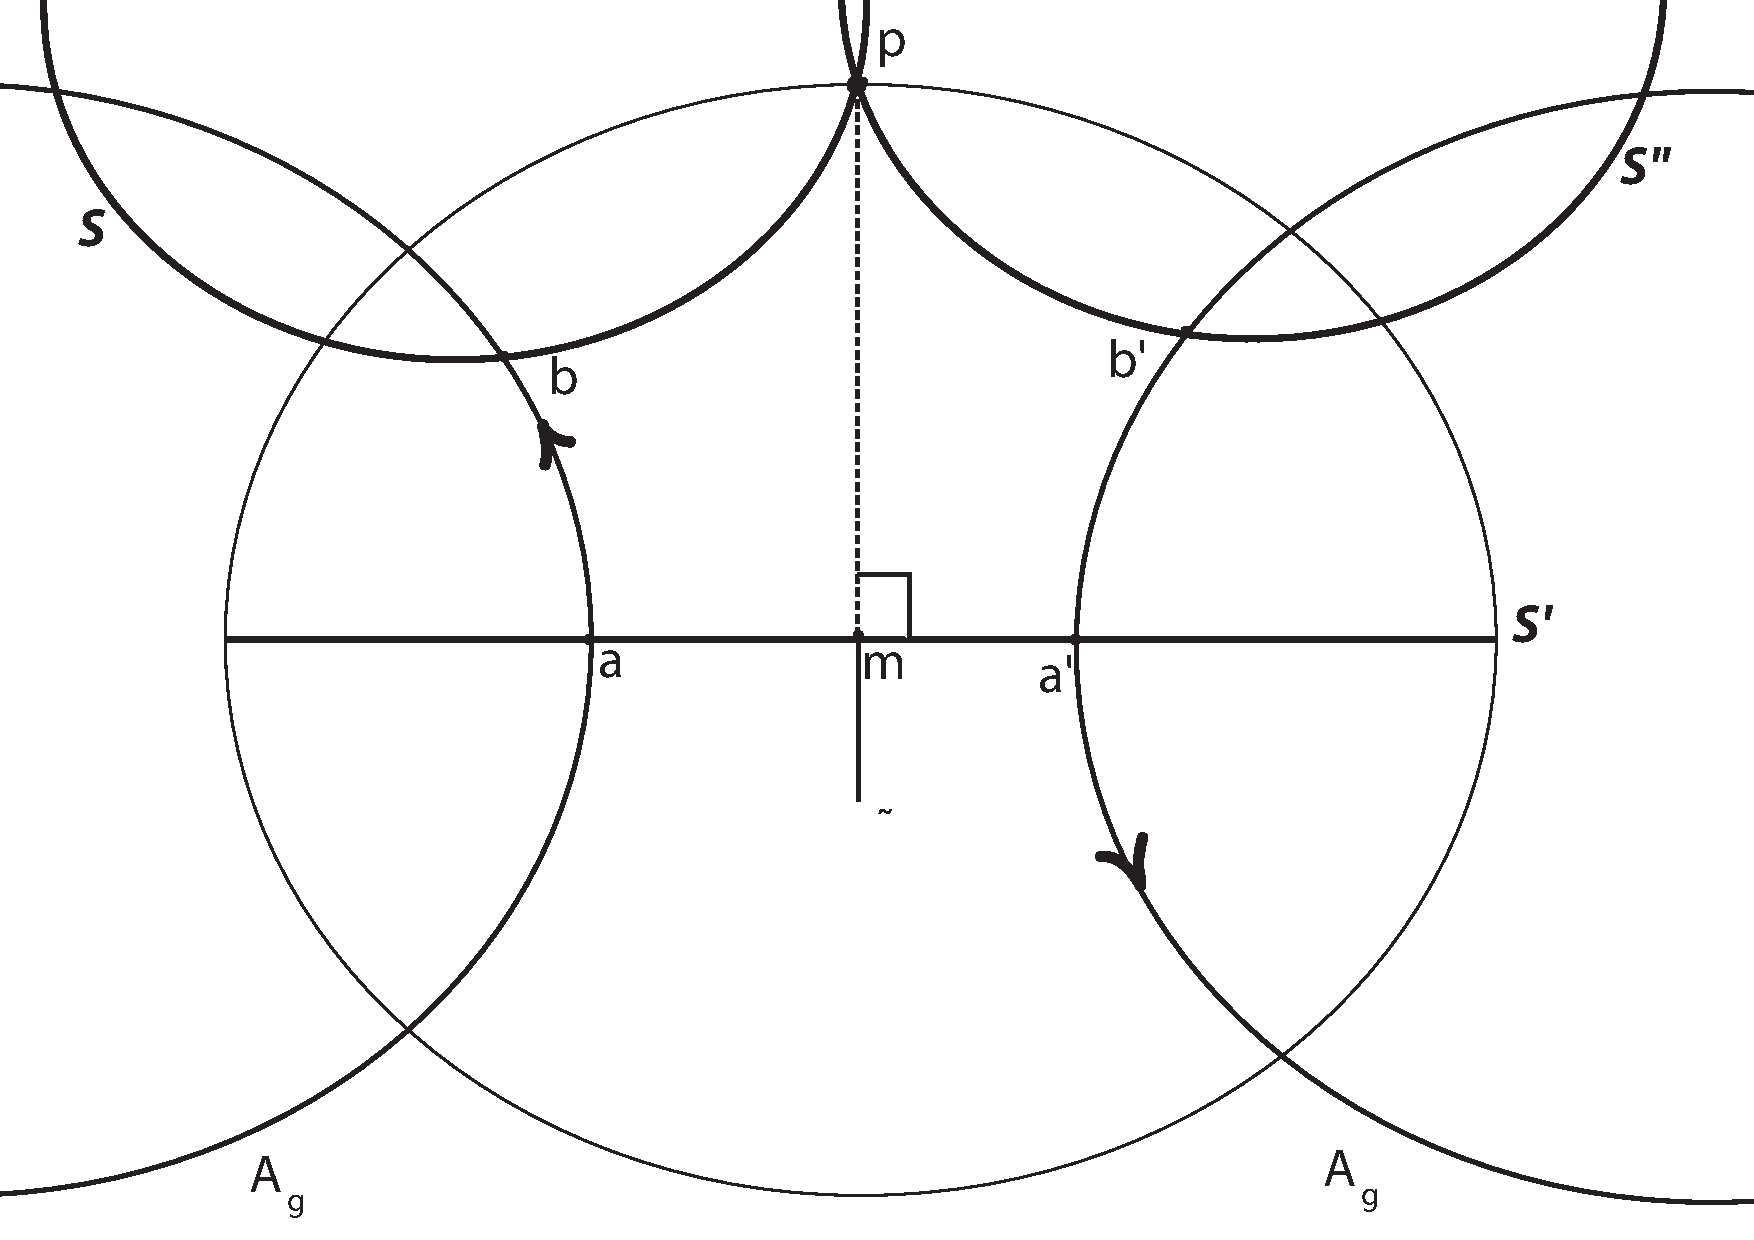
\includegraphics[width=10cm]{lemma1-dibujo4}\\
  \caption{Figura \ref{lemma1-dibujo4}}\label{lemma1-dibujo4}
\end{figure}



Luego $abpm$ es un cuadrilatero con 3 \'angulos rectos y el \'angulo
restante agudo (cuadrilatero de lambert Fig. \ref{lemma1-dibujo5}) cuyas medidas son
$\frac{1}{4} \phi_{fg}$ con lados $\frac{1}{2} \delta$ y $
\frac{1}{2} \lambda$ por lo cual tenemos $senh \frac{1}{2} \delta
senh \frac{1}{2} \lambda = cos \frac{1}{4} \phi_{fg} \leq 1$ y es
igual a 1 en el caso de que se intersecten en el infinito ( $\phi
=0$) y en dado caso la transformaci\'on seria parab\'olica. \\ \\

\begin{figure}[h]
  \centering
  % Requires \usepackage{graphicx}
  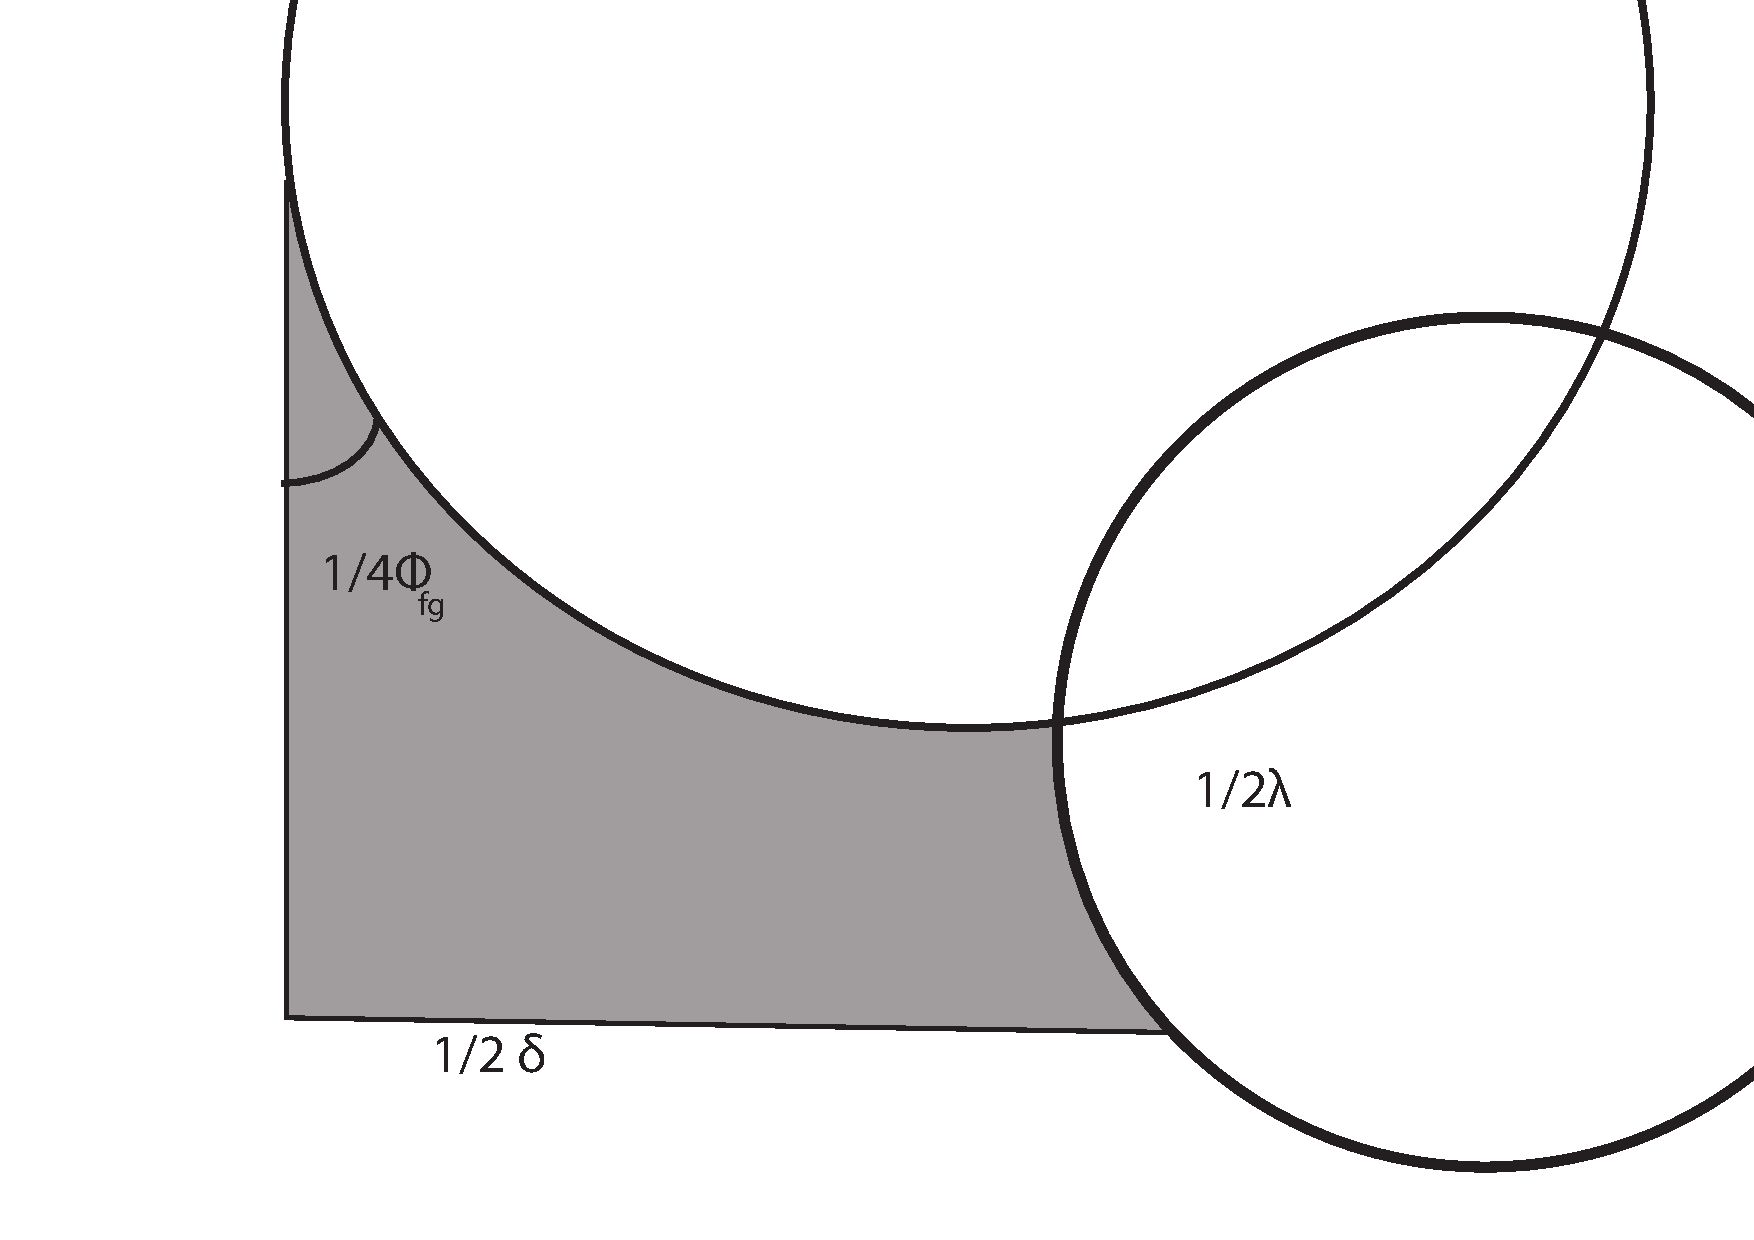
\includegraphics[width=10cm]{lemma1-dibujo5}\\
  \caption{Cuadrilatero de Lambert}  \label{lemma1-dibujo5}
\end{figure}



\textbf{Caso 2}


En el caso que los ejes sean divergentes, existe una recta normal a
ambos  y se tiene que la recta $l$ bisecta al segmento entre $s$ y
$s'$ de esta recta normal, entonces basta probar que;

\begin{enumerate}
\item Esta recta normal es el eje de $fg$
\item En efecto $l$ bisecta al segmento entre $s$ y $s'$ de esta
recta normal
\end{enumerate}

Para (1) Probaremos que $fg$ es hiperb\'olica viendo que tiene dos
puntos fijos y que se encuentran en la normal mencionada antes. Sean
$x$ y $x' $ los puntos finales de dicha recta normal y notemos que
$s''x=x'$ ya que $s''x$ debe cumplir que esta sobre la recta normal
a $s''$ y que $d_{H}(x,s'')=d_{H}(s''x,s'')$ pero $d_{H}(x,s'') =
\infty$, por la misma raz\'on $sx'=x$ entonces $ss''x=x$ y tambien
se cumple $ss''x'=x'$ por lo tanto $fg$ tiene 2 puntos fijos y su
eje es la recta que los une, que en este caso es la recta normal
mencionada (Fig. \ref{lemma1-dibujo6-2}).

\begin{figure}[h]
  \centering
  % Requires \usepackage{graphicx}
  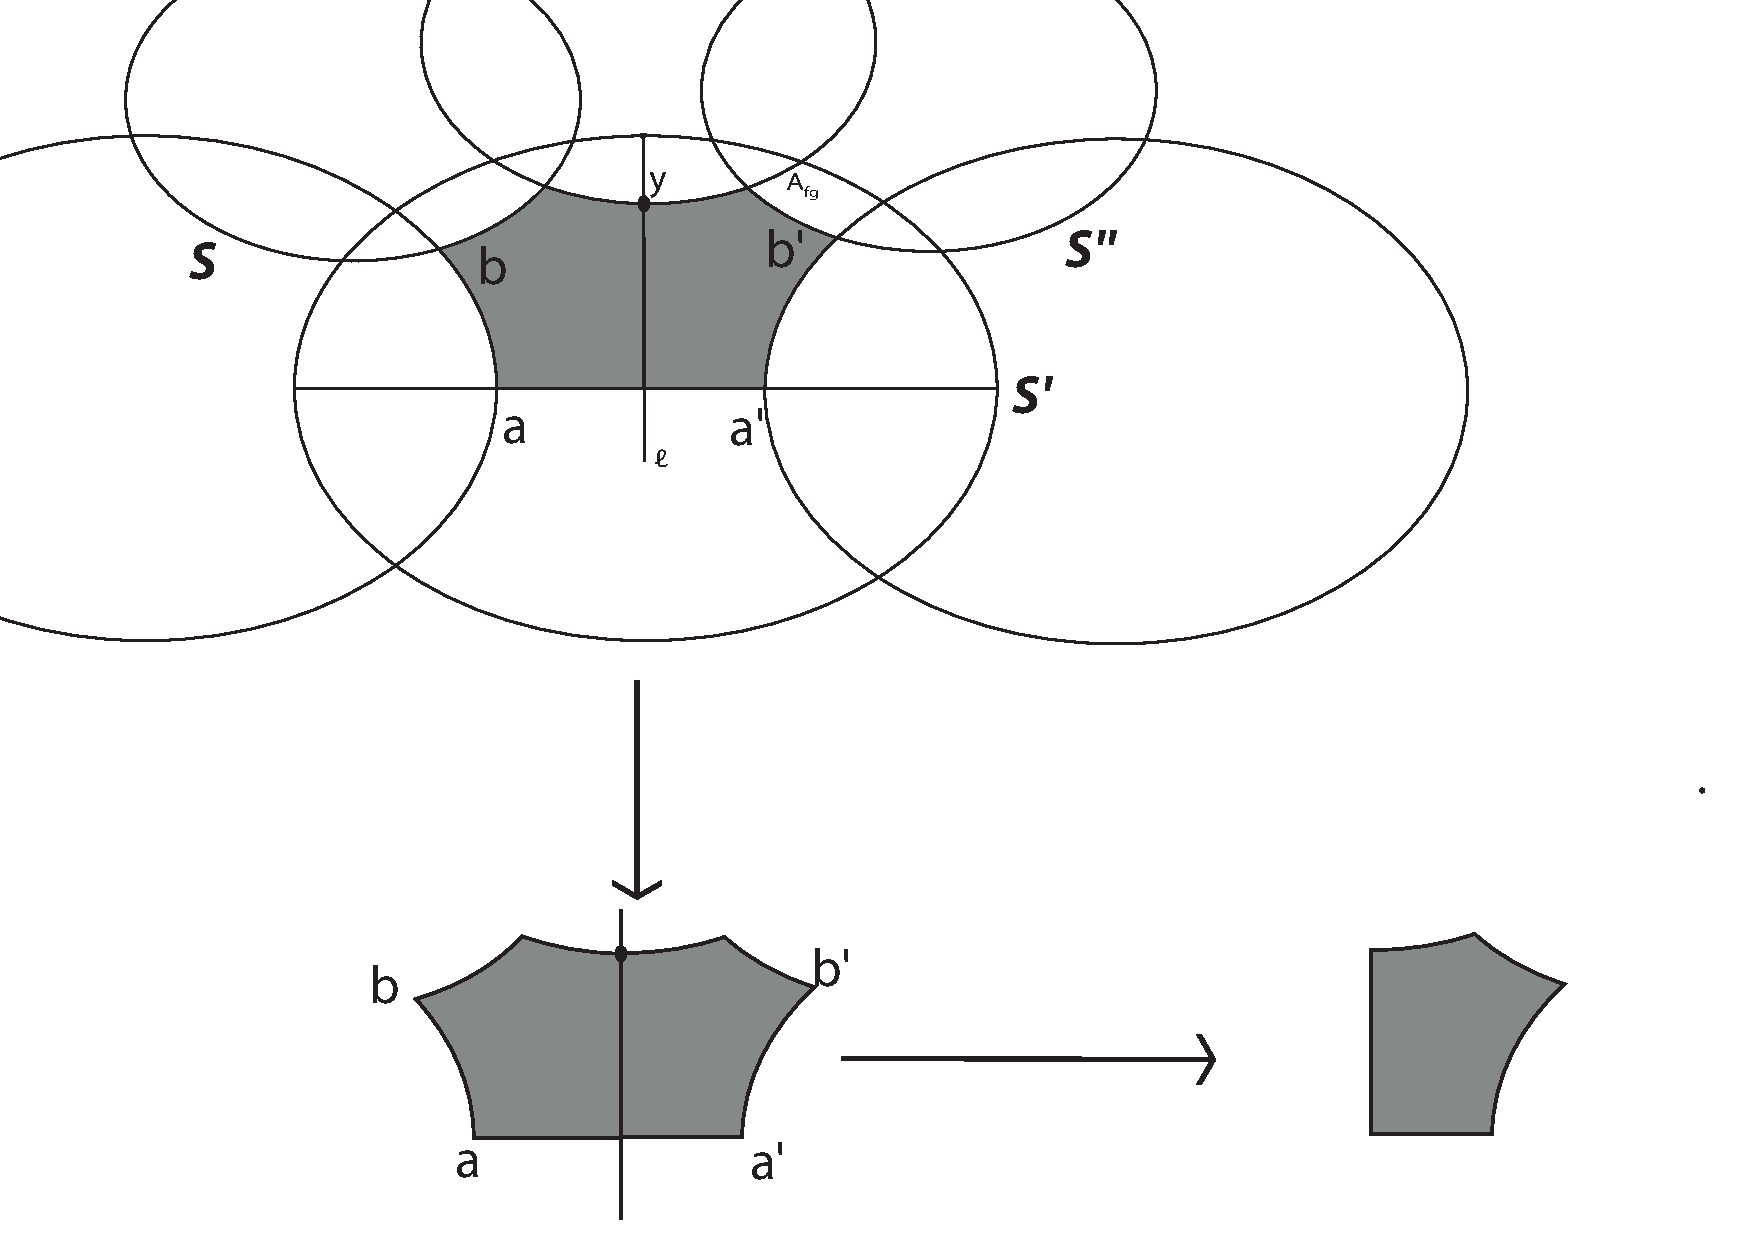
\includegraphics[width=10cm]{lemma1-dibujo6-2}\\
  \caption{Figura \ref{lemma1-dibujo6-2} }\label{lemma1-dibujo6-2}
\end{figure}


Para (2) queremos probar que $d_{H}(x,y) = d_{H}(y,x')$ donde $y$ es
el punto de intersecci\'on de la normal con $l$, al reflejar
respecto de $l$ y notando que $x \mapsto x'$ bajo $s$ y $d_{H}(x,y)
= d_{H}(y,sx)$ tenemos el resultado. \\


Finalmente tenemos las rectas $s'',A_{g},s,l$ y $A_{fg}$ y estas
forman un pentagono con 4 \'angulos rectos y con lados
$\frac{1}{2}\lambda_{fg},\frac{1}{2}\delta,\frac{1}{2}\lambda$
 (Fig. \ref{lemma1-dibujo9}) y podemos concluir (\ref{cha:apendice})
$$ senh \frac{1}{2} \delta senh \frac{1}{2} \lambda = cosh \frac{1}{4} \lambda_{fg} >1$$
$ _{\square} $

\begin{figure}[h]
  \centering
  % Requires \usepackage{graphicx}
  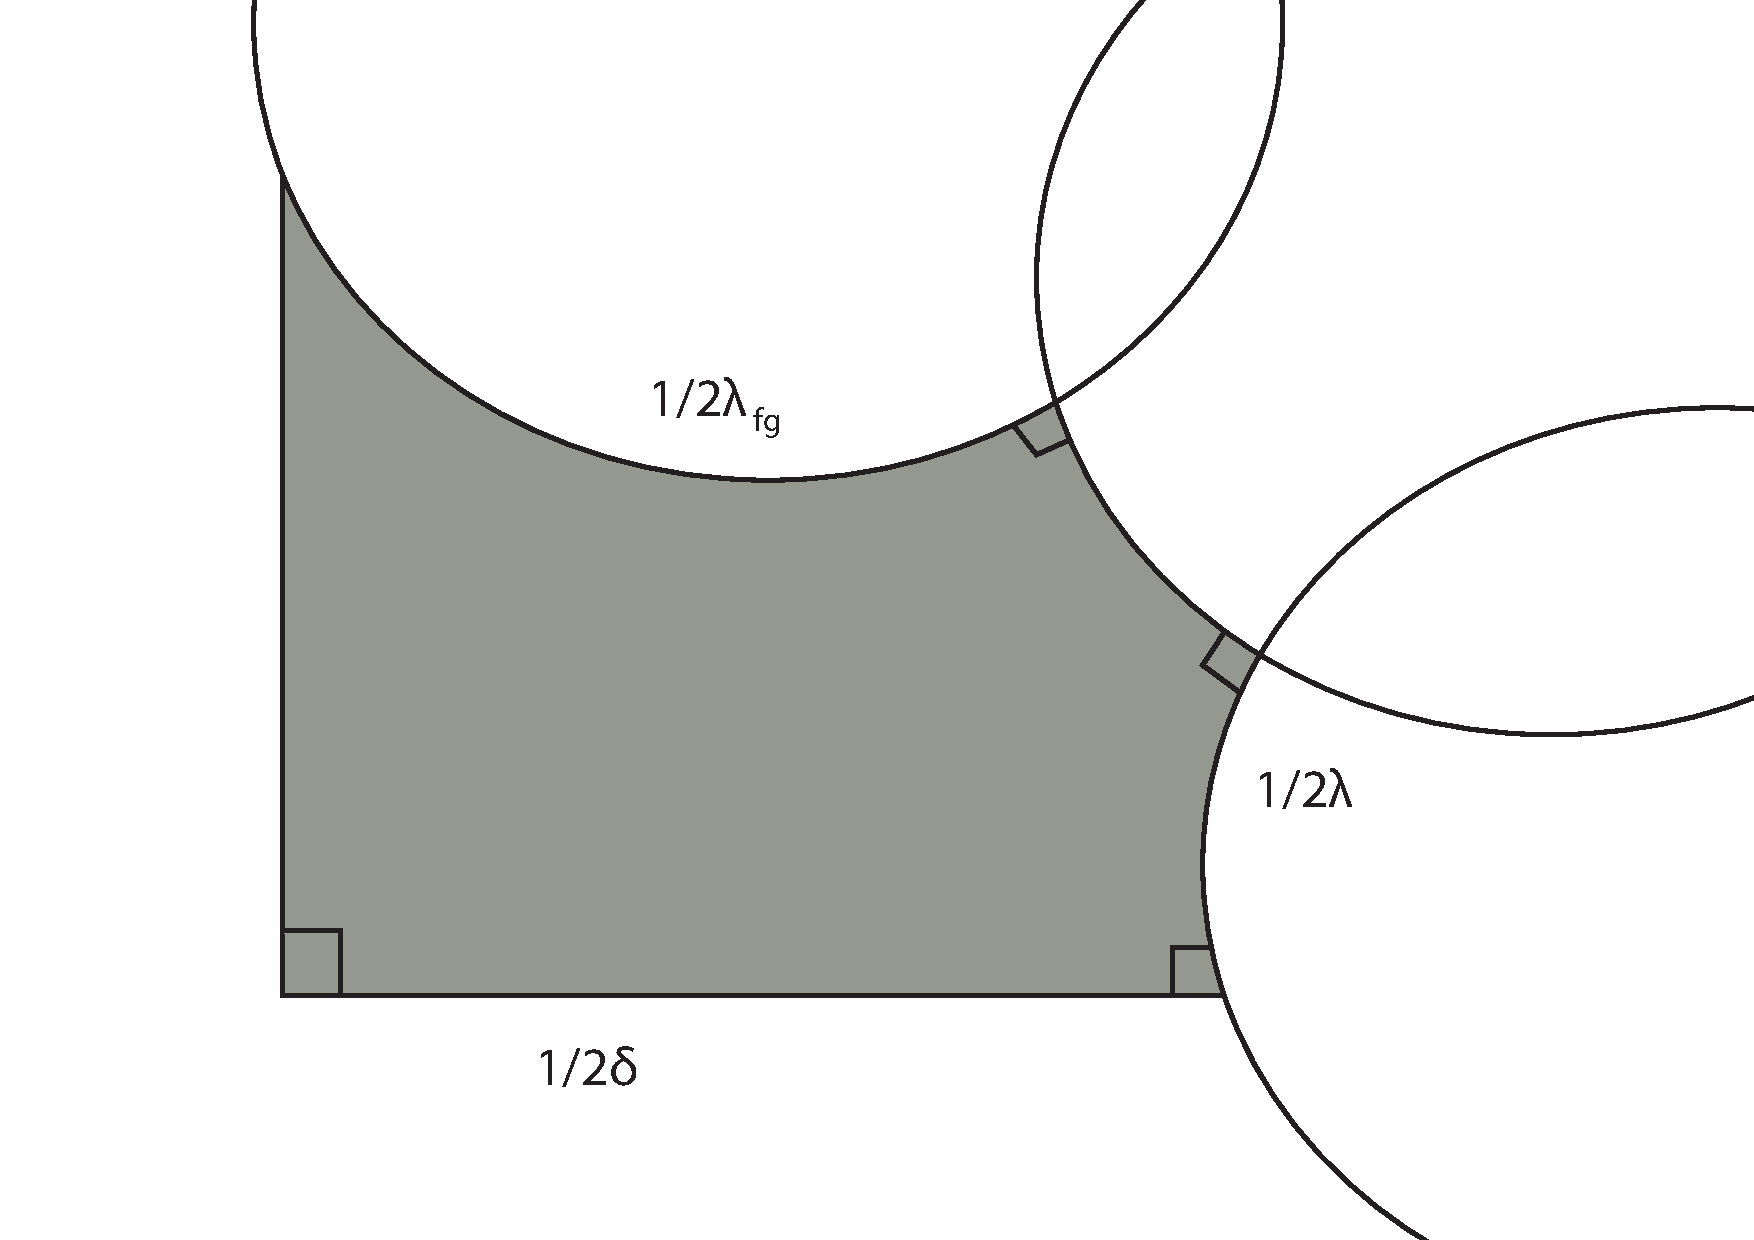
\includegraphics[width=10cm]{lemma1-dibujo9}\\
  \caption{Pent\'agono con 4 \'angulos rectos}\label{lemma1-dibujo9}
\end{figure}



\section{El lema del conmutador de los elemetos hiperb\'olicos}

\begin{lem} \label{lema2}
Sean $f$ y $g$ dos elementos hiperb\'olicos con ejes $A_{f}$ y
$A_{g}$ y desplazamientos iguales $\lambda $, y con \'angulo de
intersecci\'on $\phi $.El conmutador $[f,g]=fgf^{-1}g^{-1}$
es el\'iptico , parab\'olico o hiperb\'olico dependiendo de

$$ senh^{2}(\frac{1}{2} \lambda) sen \phi  \left \{ \begin{matrix} >1
\\ =1 \\ < 1 \end{matrix}\right. $$
\end{lem}

\textit{Prueba}:

Sea $s'$ el punto de intersecci\'on de $A_{f}$  y $A_{g}$, sea $s$
el punto sobre $A_{f}$ tal que $d_{H}(s',s)= \frac{1}{2} \lambda$ y
trazado siguiendo la direcci\'on de $A_{f}$, y sea $s''$ el punto
sobre $A_{g}$ tal que $d_{H}(s',s'')=\frac{1}{2} \lambda$ y trazado
siguiendo la misma direcci\'on que $A_{g}$ (Fig. \ref{lemma2-dibujo1}). \\

\begin{figure}[h]
  \centering
  % Requires \usepackage{graphicx}
  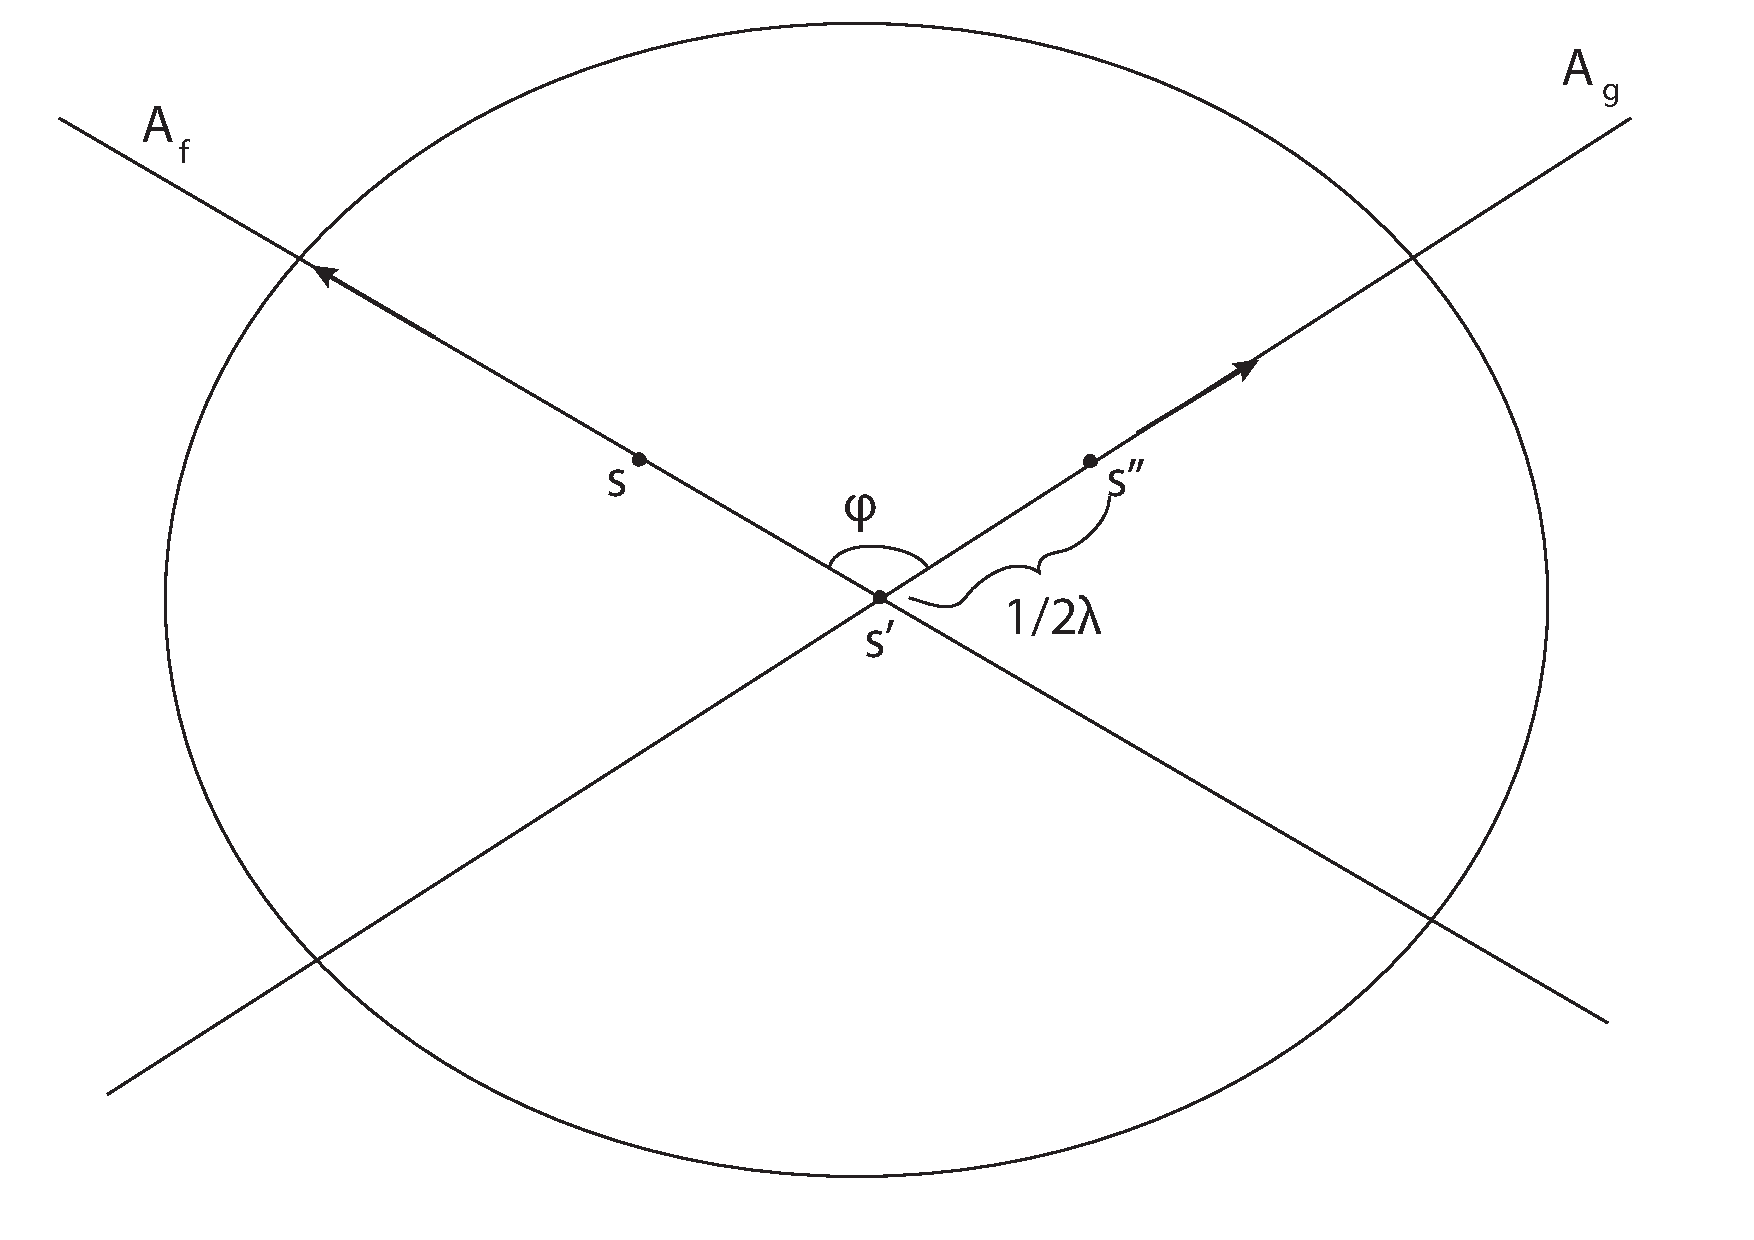
\includegraphics[width=10cm]{lemma2-dibujo1}\\
  \caption{Figura \ref{lemma2-dibujo1}}\label{lemma2-dibujo1}
\end{figure}


Y consideremos los elementops el\'ipticos de \'angulo $\pi$  respecto a estos puntos
y los denotaremos igual que denotamos a sus puntos fijos. \\

Queremos primero probar que $f=ss'$, para esto deseamos ver los puntos que deja fijos $ss'$. El elemento el\'iptico con \'angulo $\pi$ funciona de la
siguiente manera; dado un punto $x$ se traza la recta que va de $x$
al punto fijo $c$,la im\'agen de $x$ bajo el elemento el\'iptico llamemosle $y$ esta
sobre la misma recta y $d_{H}(x,c)=d_{H}(y,c)$, con este proceso
podemos ver que $ss'$ fija los mismos puntos que $f$ por lo tanto el
eje de $f$ es el mismo que el  de $ss'$ solo falta ver cuanto es el
desplazamiento de $ss'$,como antes, basta verificarlo para un
punto y en esta ocasi\'on tomamos el punto $s'$, tenemos que
$d_{H}(s,ss'(s'))=d_{H}(s,s(s'))= 2d_{H}(s',s)=2(\frac{1}{2}
\lambda)= \lambda $ por lo tanto $f=ss'$. Un proceso an\'alogo nos
enseña que $g=s's''$ y como $s's'$ es la indentidad entonces $fg
= ss''$, m\'as a\'un $f^{-1} = s's,g^{-1}=s''s'$ y entonces
$f^{-1}g^{-1}= s'ss''s'=s'fgs'=s'fgs'^{-1}$, luego $ss'$ es un
elemento hiperb\'olico con recta invariante igual a la recta que pasa por
$s$ y $s''$ y desplazamiento $2d_{H}(s,s'')$, m\'as a\'un
$f^{-1}g^{-1}$ es hiperb\'olico obtenido de $fg$ conjungando por
$s'$, tenemos entonces;

\begin{enumerate}
\item $f^{-1}g^{-1}$ tiene un desplazamiento con la misma medida que
$fg$
\item su eje $A_{f^{-1}g^{-1}}$ se obtiene de $A_{fg}$ rotando por $s'$.
\end{enumerate}

Para probar (1) queremos ver cuanto mide $d_{H}(x,s'fgs'x)$ y
tenemos que $d_{H}(x,s'fgs'x)= d_{H}(s'x,fg(s'x))$ y esta \'ultima
cantidad es el desplazamiento de $fg$. \\ \\

(2) se cumple  ya que $f^{-1}g^{-1} (s'A_{fg})= s'fgs'(s'A_{fg})=
s'fg(A_{fg})=s'A_{fg}$. \\

Entonces estos ejes son divergentes y sus correspondientes
transformaciones tienen sentidos opuestos, aplicamos entonces el
\textbf{lema} \ref{lema1} a $fg$ y a $f^{-1}g^{-1}$ entonces $[f,g]$ es
el\'iptico , parab\'olico o hiperb\'olico seg\'un sea

$$senh \eta senh \frac{1}{2} \lambda_{fg} \lesseqgtr 1$$

Donde $\eta$ es la perpendicular desde $s'$ en el tri\'angulo
$ss's''$ (Fig. \ref{lemma2-dibujo4}) y por trigonometr\'ia hiperb\'olica (\ref{cha:apendice}) se cumple $senh \eta
senh\frac{1}{2} \lambda_{fg} = sen \phi senh^{2} \frac{1}{2}\lambda$
$_{\square}$

\begin{figure}[h]
  \centering
  % Requires \usepackage{graphicx}
  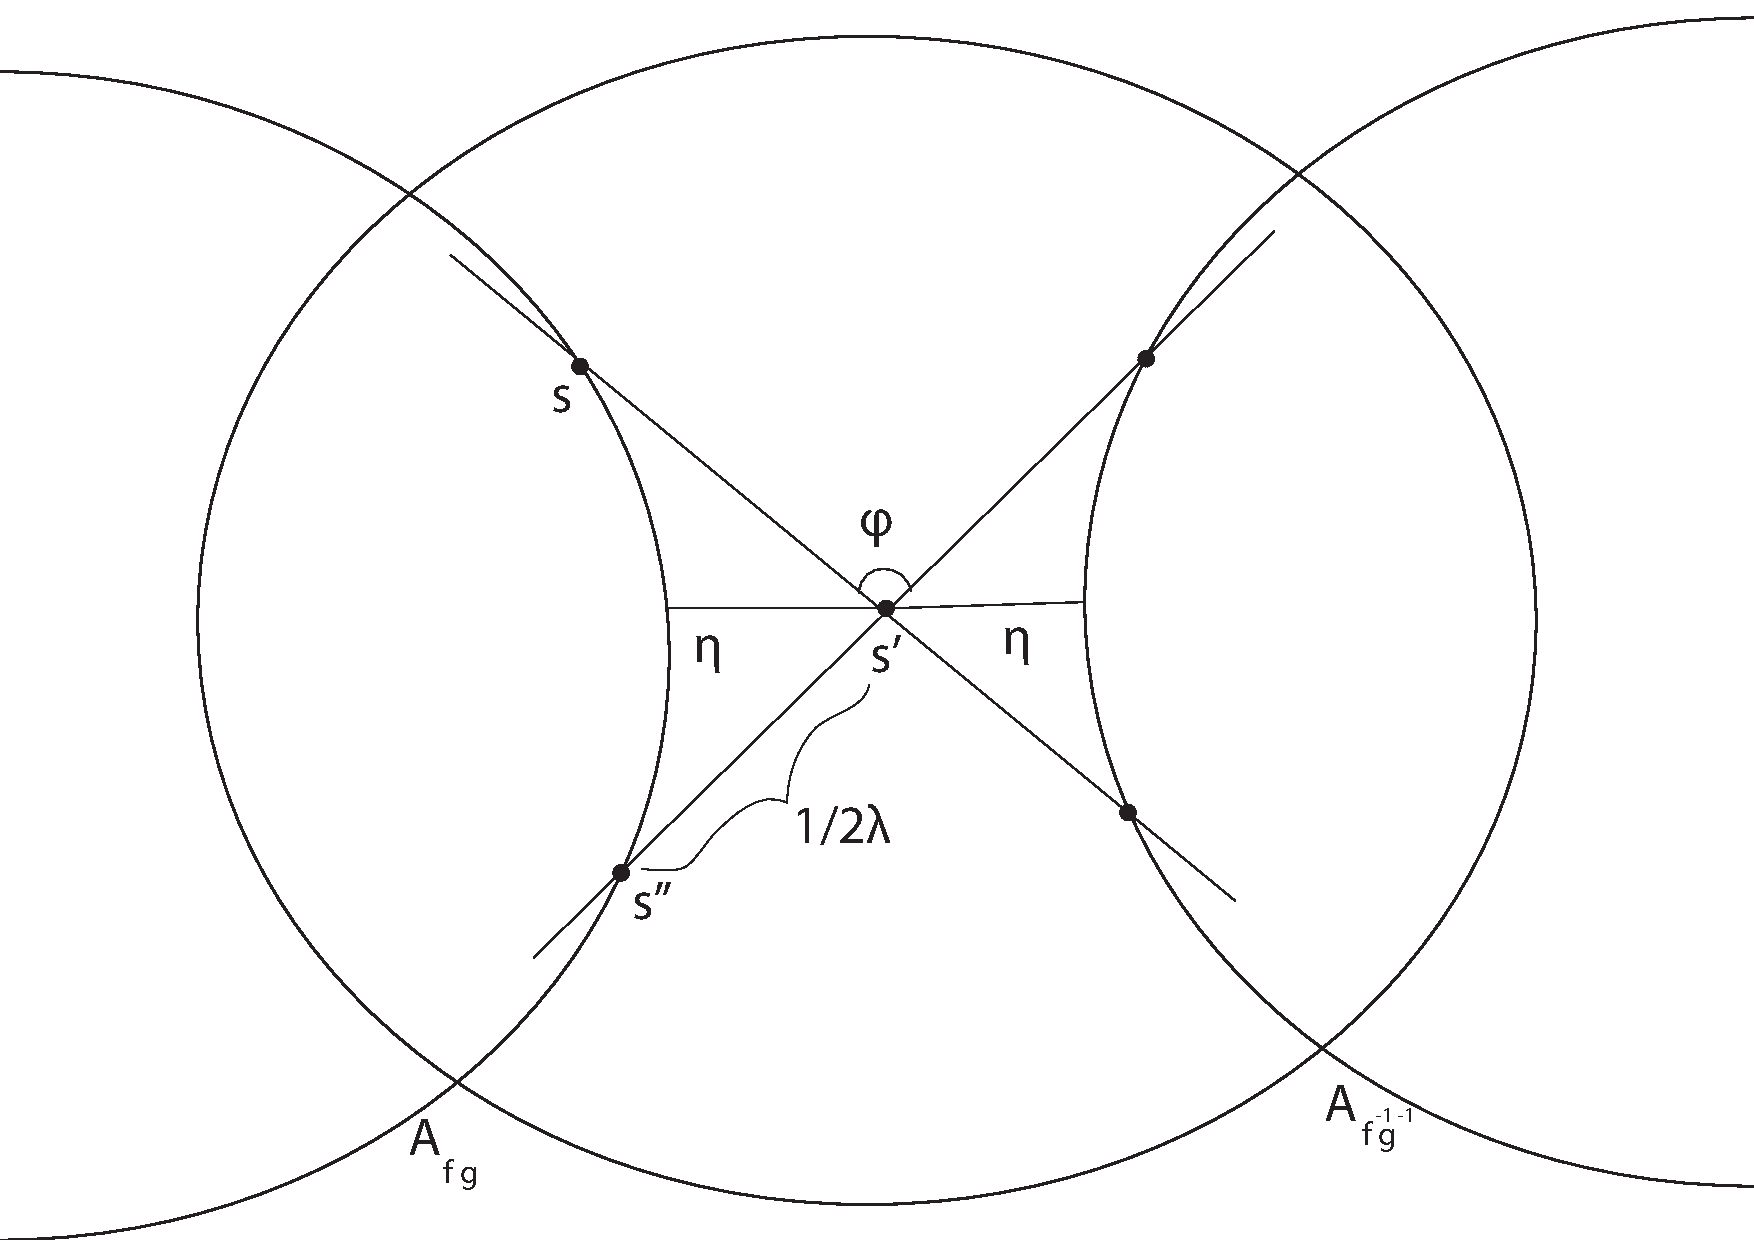
\includegraphics[width=7cm]{lemma2-dibujo4}\\
  \caption{Figura \ref{lemma2-dibujo4}}\label{lemma2-dibujo4}
\end{figure}


\section{El lema del conmutador de los elementos parab\'olicos}

\begin{lem}\label{lema3}
Sean $f,g$ elementos parab\'olicos con puntos fijos $c_{f}$ y
$c_{g}$ entonces el conmutador $[f,g]$ es hiperb\'olico.
\end{lem}

\emph{Prueba.} \\

\begin{figure}[h]
  \centering
  % Requires \usepackage{graphicx}
  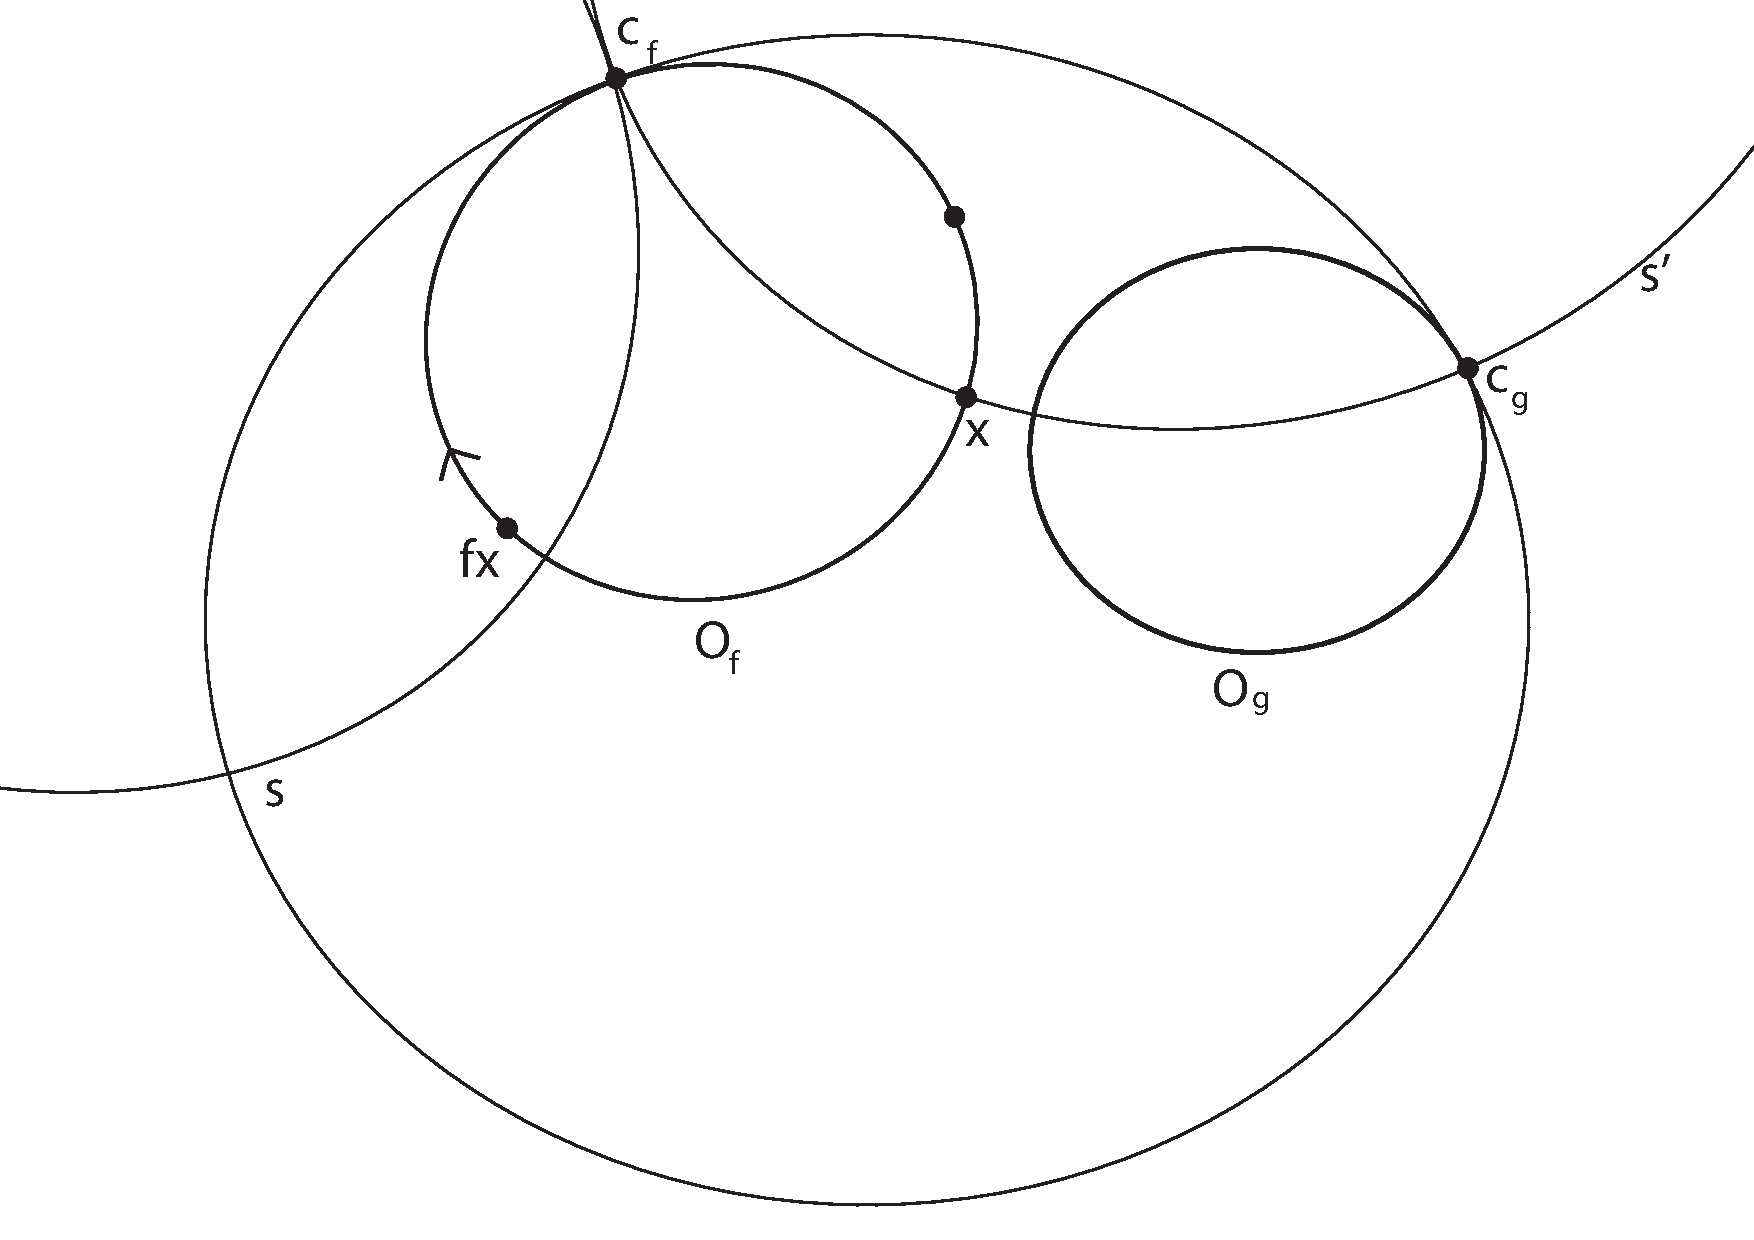
\includegraphics[width=10cm]{lemma3-dibujo1}\\
  \caption{Figura \ref{lemma3-dibujo1}}\label{lemma3-dibujo1}
\end{figure}


 Sea $s'$ la recta que une $c_{f}$ y $c_{g}$ y denotemos la reflexi\'on respecto a esta recta
tambi\'en como $s'$. Sea $O_{f}$ un horociclo dado con punto al
infinito $c_{f}$, y $x \in O_{f}$, tomamos $s$ en el conjunto de geod\'esicas que pertenece al haz parab\'olico con punto fijo $c_{f}$ (\cite{Beardon}).

Tenemos entonces que $ f=ss' $, y analogamente obtenemos  que existe
$s''$ tal que $g=s's''$ luego tenemos
$[f,g]=ss''s'ss''s'=(ss''s')^{2}$, la composici\'on de reflexiones
conserva el sentido por lo tanto la composici\'on de 3 reflexiones
invierte el sentido y es por tanto una reflexi\'on o una
h-reflexi\'on entonces su cuadrado es la identidad o un elemento
hiperb\'olico.Probemos que  $f$ y $g$ no permutan: Si $fg=gf$, tenemos que $f$ deja invariante el conjunto de puntos fijos de $g$ y vicerversa, para ver esto sea $x$ un punto fijo de $f$ entonces $f(g(x))= g(f(x)) = g(x)$, es decir $g(x)$ es un punto fijo de $f$, si sustituimos $g$ por $g^{-1}$ analogamente obtenemos que $g^{-1}(x)$ es un punto fijo, es decir todo punto fijo es la imagen bajo $g$ de otro punto fijo ( $x= g(g^{-1}(x))$). Dado esto $[f,g]$ es la identidad si y solo si $f$ y $g$ conmutan, como hemos probado que esto no es posible se tiene que $[f,g]$ es un elemento hiperb\'olico. $_{\square}$

\section{El lema del conmutador de los elementos hiperb\'olicos con ejes paralelos}

\begin{lem} \label{lema4}
Sean $f$ y $g$ elementos hiperb\'olicos con ejes paralelos y con
punto com\'un $u$, entonces el conmutador $[f,g]$ es un elemento
parab\'olico con centro en $u$
\end{lem}

\begin{figure}[h]
  \centering
  % Requires \usepackage{graphicx}
  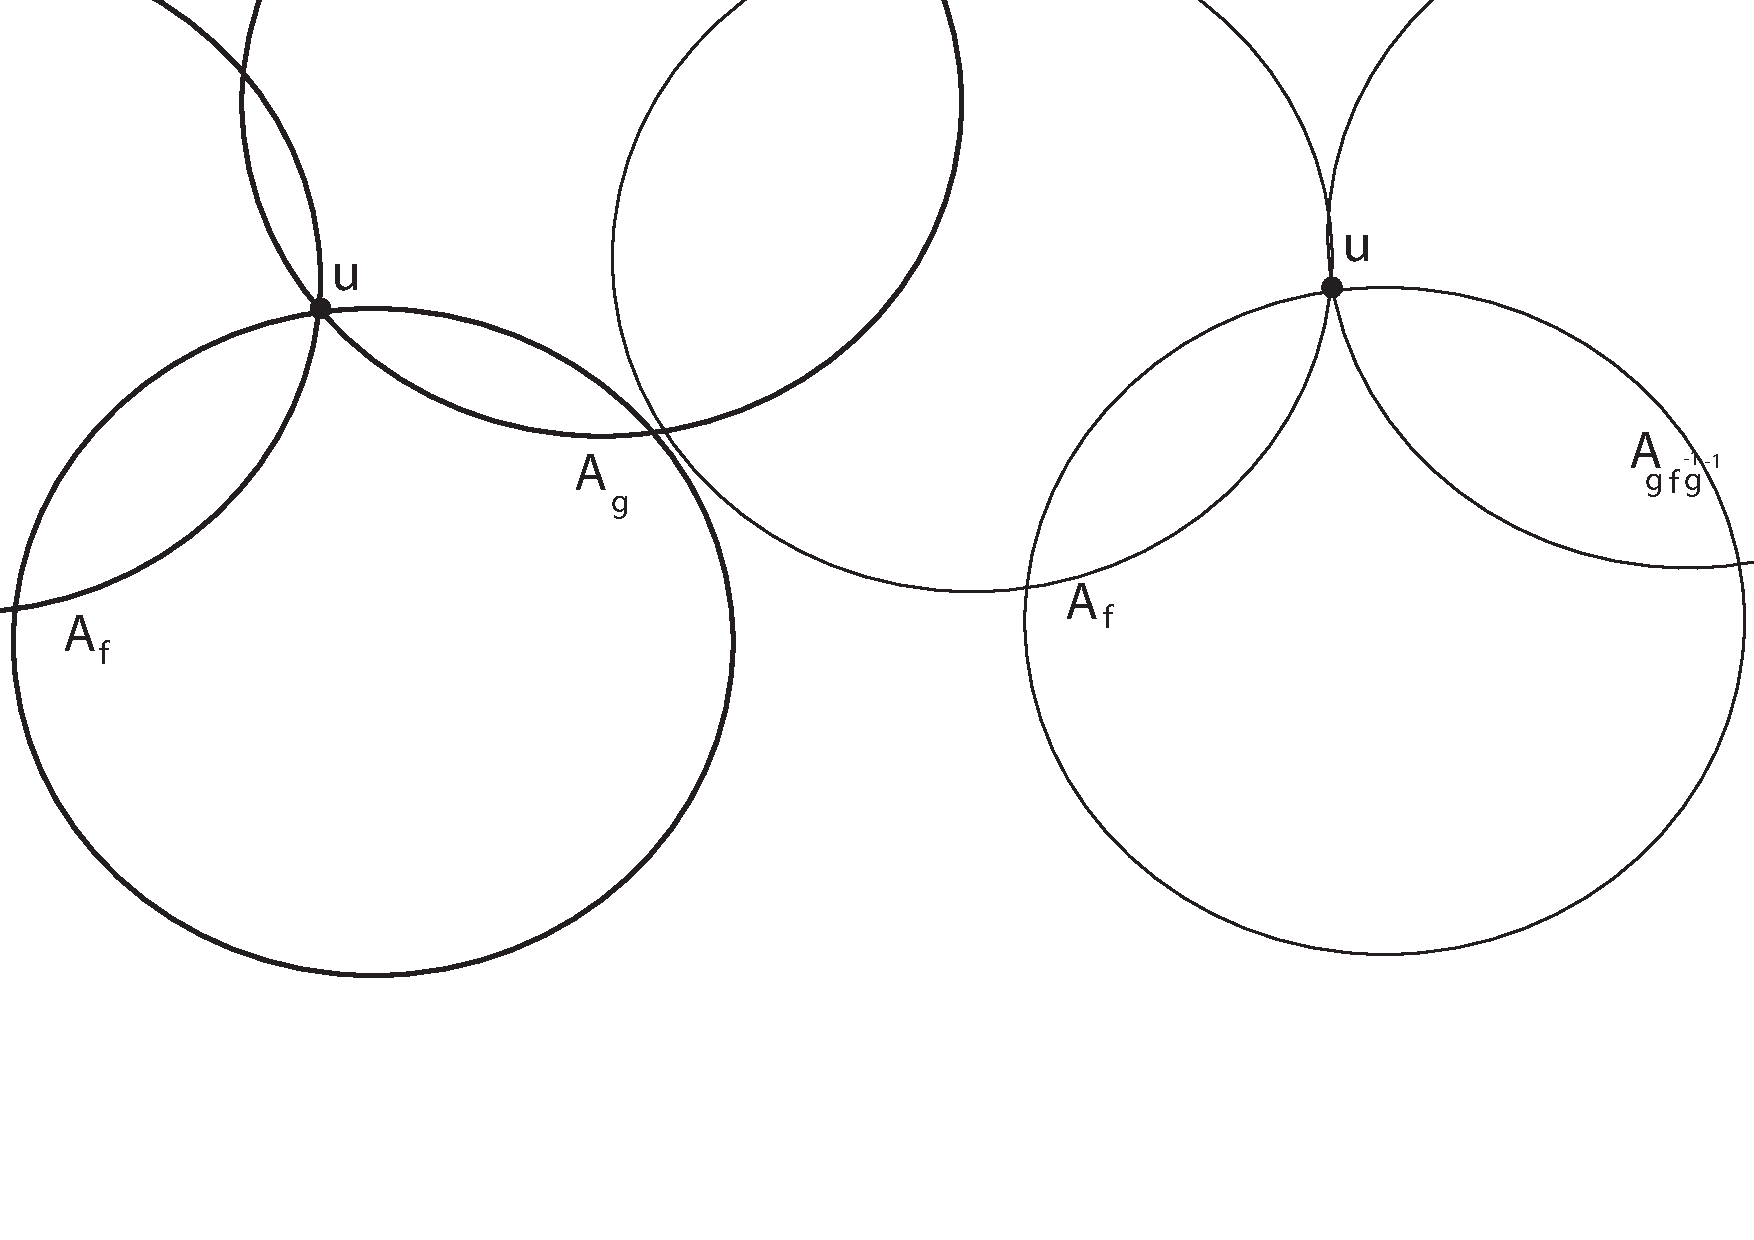
\includegraphics[width=10cm]{lemma4-dibujo1}\\
  \caption{Figura \ref{lemma4-dibujo1}}\label{lemma4-dibujo1}
\end{figure}



\textit{Prueba}:

Primero veamos que  $f \neq gf^{-1}g^{-1}$, es claro que
$gf^{-1}g^{-1}$ fija $u$ ya que tanto $f$ como $g$ lo fijan, sea $x$
el punto final del eje de $f$ distinto de $u$, es claro que $g^{-1}$
no fija este punto, y $gx \neq u$ (puesto que $g^{-1}u \neq x$)
concluimos con esto $f \neq gf^{-1}g^{-1}$.

Sin perdida de generalidad podemos suponer que $u=0$ y que las matrices de los elementos hiperb\'olicos correspondientes a $f$ y $g$ lucen de la siguiente manera:

$$M_{f}=    \begin{pmatrix}
 a& 0\\
 c & d
 \end{pmatrix} \  ,  \ M_{g} =     \begin{pmatrix}
 x& 0\\
 w& z
 \end{pmatrix}   $$

 Donde $ad=1,xz=1$ , $|a+d|>2$ y $|x+z|>2$. Haciendo los c\'alculos obtenemos que $tr (M_{f}M_{g}M_{f^{-1}}M_{g^{-1}})=2$ por lo que el conmutador es un elemento parab\'olico con punto fijo $u=0$. $_{\square}$

%Primero veamos que  $f \neq gf^{-1}g^{-1}$, es claro que
%$gf^{-1}g^{-1}$ fija $u$ ya que tanto $f$ como $g$ lo fijan, sea $x$
%el punto final del eje de $f$ distinto de $u$, es claro que $g^{-1}$
%no fija este punto, y $gx \neq u$ (puesto que $g^{-1}u \neq x$)
%concluimos con esto $f \neq gf^{-1}g^{-1}$, claramente su
%desplazamiento mide lo mismo (debido a que $g$ es isometria) pero
%con sentidos opuestos (ya que $gf^{-1}g^{-1}$ respeta el sentido de
%$f^{-1}$). (\textcolor[rgb]{1.00,0.00,0.00}{dibujo})
%(\textcolor[rgb]{0.00,0.00,1.00}{inconcluso}).

\section{El lema del elemento el\'iptico}

\begin{lem} \label{lema5}
Si en un grupo $G < PSL(2,\mathbb{R})$ sin puntos invariantes, 2
ejes de elementos hiperb\'olicos son paralelos entonces el grupo
contiene un elemento el\'iptico
\end{lem}


\textit{Prueba}:


Del Lema \ref{lema4} tenemos que $G$ contiene elementos parab\'olicos
y con punto en com\'un $u$ como centro. \\

Consideremos un Horociclo $K$ con punto en el infinito $u$, sobre $K$
el elemento parab\'olico tiene un desplazamiento fijo . \\

\begin{figure}[h]
  \centering
  % Requires \usepackage{graphicx}
  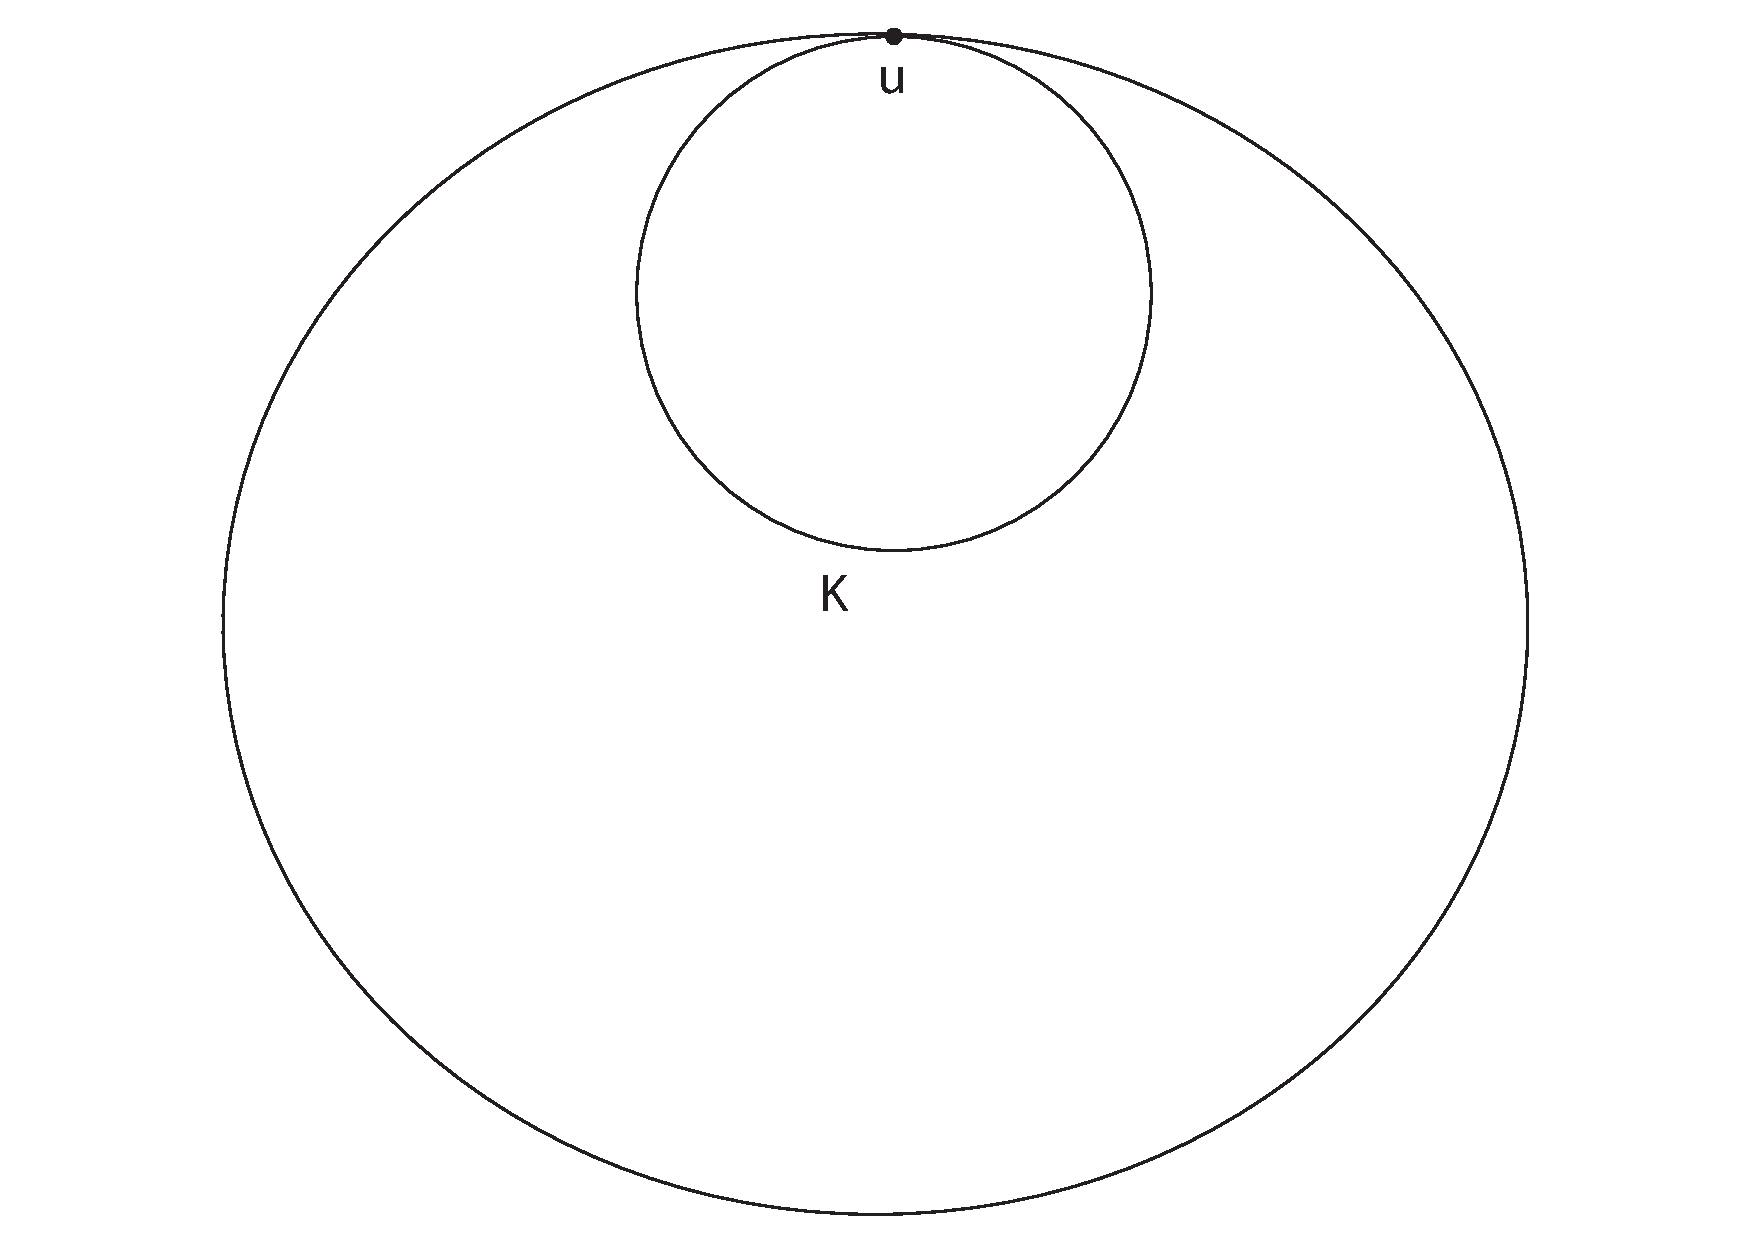
\includegraphics[width=10cm]{lemma5-dibujo1}\\
  \caption{Figura \ref{lemma5-dibujo1}}\label{lemma5-dibujo1}
\end{figure}


Sea $S_{u} < G$ el subgrupo de $G$ que consta de elementos
parab\'olicos con punto en el infinito $u$ y sea $x \in K$, la clase
de equivalencia $S_{u}x$ es un subconjunto de $K$ y podemos
distinguir dos casos.

\begin{enumerate}
\item Los puntos forman una sucesi\'on de puntos equidistantes
cuando $S_{u}$ es dinscontinuo.

\item El conjunto de puntos es denso en todo $K$ cuando $S_{u}$ no
es discontinuo.
\end{enumerate}

Para probar (1), sea $d=min \lbrace d_{H}(x,fx) | f \in S_{u}
\rbrace$ este minimo existe por que si no es asi se tendria un punto
de acumulaci\'on lo cual por hip\'otesis no es posible. Si $y \in
S_{u}x $ es claro que $min \lbrace d_{H}(y,fy) | f \in S_{u} \rbrace
= d$ y de esto concluimos que el conjunto de puntos es equidistante
de distancia $d$. \\

Para el caso (2) por hip\'otesis tenemos que $S_{u}x$ se acumula en
$x$ y queremos ver que se acumula en todo $K$. Sea $k \in K$ un
punto arbitrario y $B_{\epsilon}(k)= \lbrace z \in D| d_{H}(k,z) < \epsilon
\rbrace$ y tomemos $B_{\epsilon}(k) \cap K$, queremos ver que esxiste $x
\in S_{u}x$ tal que $d_{H}(k,x) < \epsilon$ , si dicha $x$ no existe
entonces los desplazamientos  en $K$ de los elementos de $S_{u}$
estarian acotados inferiormente por $\epsilon$ lo cual implicar\'ia que
$S_{u}$ es discontinuo lo que contradice la hip\'otesis, por lo
tanto $S_{u}$ en denso en todo $K$. \\

Ahora supongamos que estamos en el caso (1) y sea $g_{0}$ el
elemento con el menos desplazamiento respecto de $K$
(Fig. \ref{lemma5-dibujo2}) y $f$ un elemento
hiperb\'olico en $G$ tal que su eje $A_{f}$ tiene a $u$ como punto
fijo y cuyo sentido es tal que se aleja de $u$, entonces $fg_{0}f^{-1}$
fija $u$ y es un elemento parab\'olico y por tanto $fg_{0}f^{-1} \in
S_{u}$. \\

\begin{figure}[h]
  \centering
  % Requires \usepackage{graphicx}
  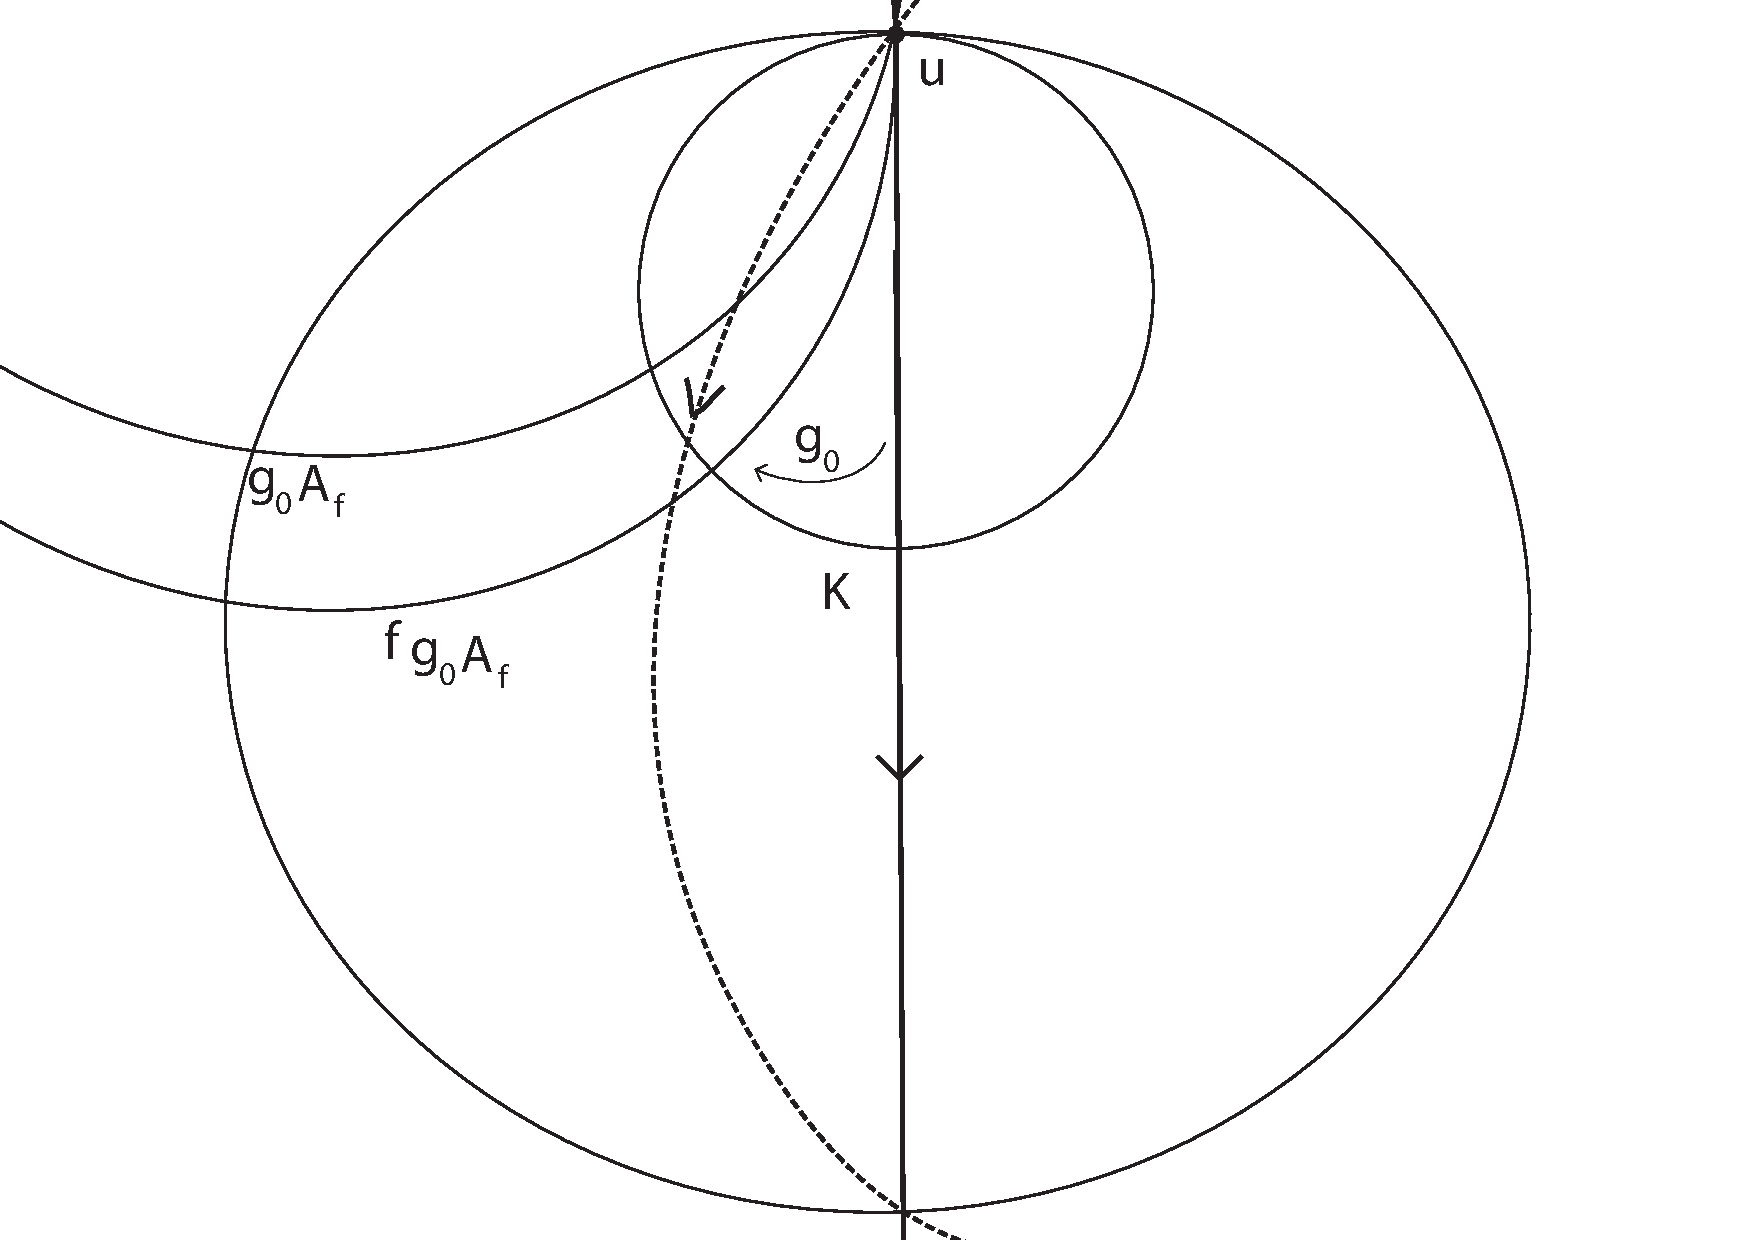
\includegraphics[width=10cm]{lemma5-dibujo2}\\
  \caption{Hiperciclo punteado }\label{lemma5-dibujo2}
\end{figure}

La imagen de $A_{f}$ bajo $fg_{0}f^{-1}$ es claramente la misma que
la de su imagen bajo $fg_{0}$, la recta $fg_{0}A^{f}$ se encuentra
entre $A_{f}$ y $g_{0}A_{f}$, luego el desplazamiento de $fg_{0}f^{-1}$
es menor que el de $g_{0}$ lo cual es una contradicci\'on, por lo
tanto $S_{u}x$ es denso en $K$, es decir los desplazamientos de los
elementos de $S_{u}$ son tan pequeños como se quiera. \\


Como $G$ no tiene a $u$ como punto invariante, sea $g \in G$ tal que
$gu \neq u$. Sean $f_{1},f_{2}$ elementos hiperb\'olicos
pertenecientes a los dos ejes del lema, al menos uno de los
elementos hiperb\'olicos $gf_{j}g^{-1}$ no fija $u$, ya
que $g$ solo puede mover $u$ a los m\'as a uno de los puntos
extremos de $A_{f_{j}}$. Entonces existe en $G$ un elemento
hiperb\'olico $f$ que no deja $u$ invariante. Elijamos ahora un
horociclo $K$ tal que intersecte $A_{f}$ (fig \ref{lemma5-dibujo3}) y elegimos $h$ tal que su
desplazamiento respecto a $K$ ayude a que los ejes $A_{f}$ y
$A_{hf}$ de $f$ y $f'=hfh^{-1}$ respectivamente se intersecten en un
\'angulo arbitrariamente pequeño, en particular elegimos $h$ tal
que
$$sen\phi senh^{2} \frac{1}{2} \lambda_{f} < 1$$

\begin{figure}[h]
  \centering
  % Requires \usepackage{graphicx}
  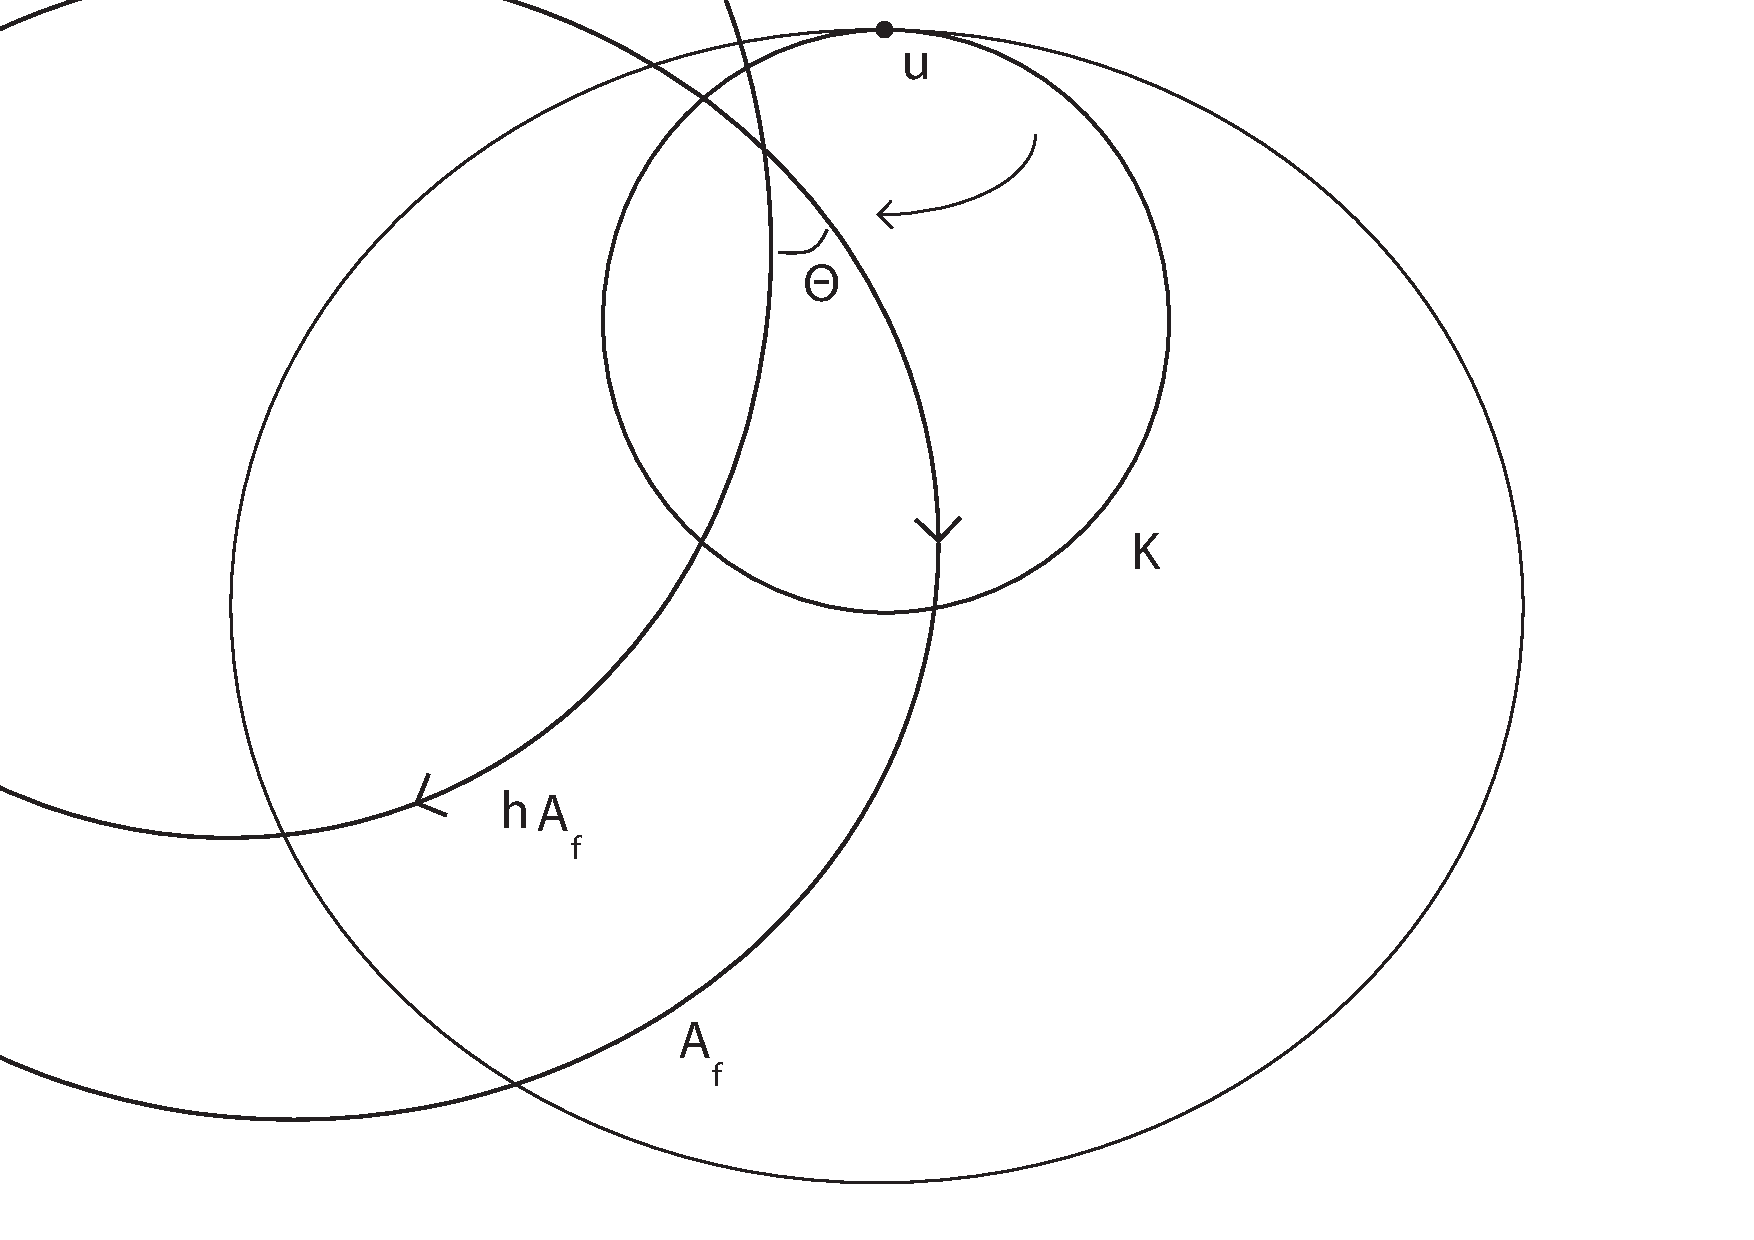
\includegraphics[width=10cm]{lemma5-dibujo3}\\
  \caption{Figura \ref{lemma5-dibujo3}}\label{lemma5-dibujo3}
\end{figure}


Ya que $senh^{2} \frac{1}{2}\lambda_{f}$ es fijo y $sen\phi
\rightarrow 0$ cuando $\phi \rightarrow 0$, y del \textbf{lema} \ref{lema2} se
sigue que $[f,f']$ es el\'iptico. $_{\square}$ \\ \\


\section{El teorema de Nielsen}

Probamos ahora la parte restante del teorema de Nielsen.

Sea $G < PSL(2,\mathbb{R})$ sin puntos invariantes y sin
elementos el\'ipticos. \\

Antes que nada veamos que $G$ no es abeliano. Si los ejes son
divergentes y  $fg = gf$ entonces $fgf^{-1} = g$, pero no es posible
ya que $fgf^{-1}$ fija $fx,fy$ con $x,y $ puntos fijos de $g$, pero
esto implica $fx=y$ y $fy=x$ pero esto implica $f^{2}x=x$, pero
$f^{2}$ fija los mimos puntos que $f$ por tanto no puede fijar los
puntos de $g$. \\

Es an\'alogo si los ejes son paralelos ya que $f$ no puede
intercambiar $x$ y $y$ al mismo tiempo. \\


\begin{figure}[h]
  \centering
  % Requires \usepackage{graphicx}
  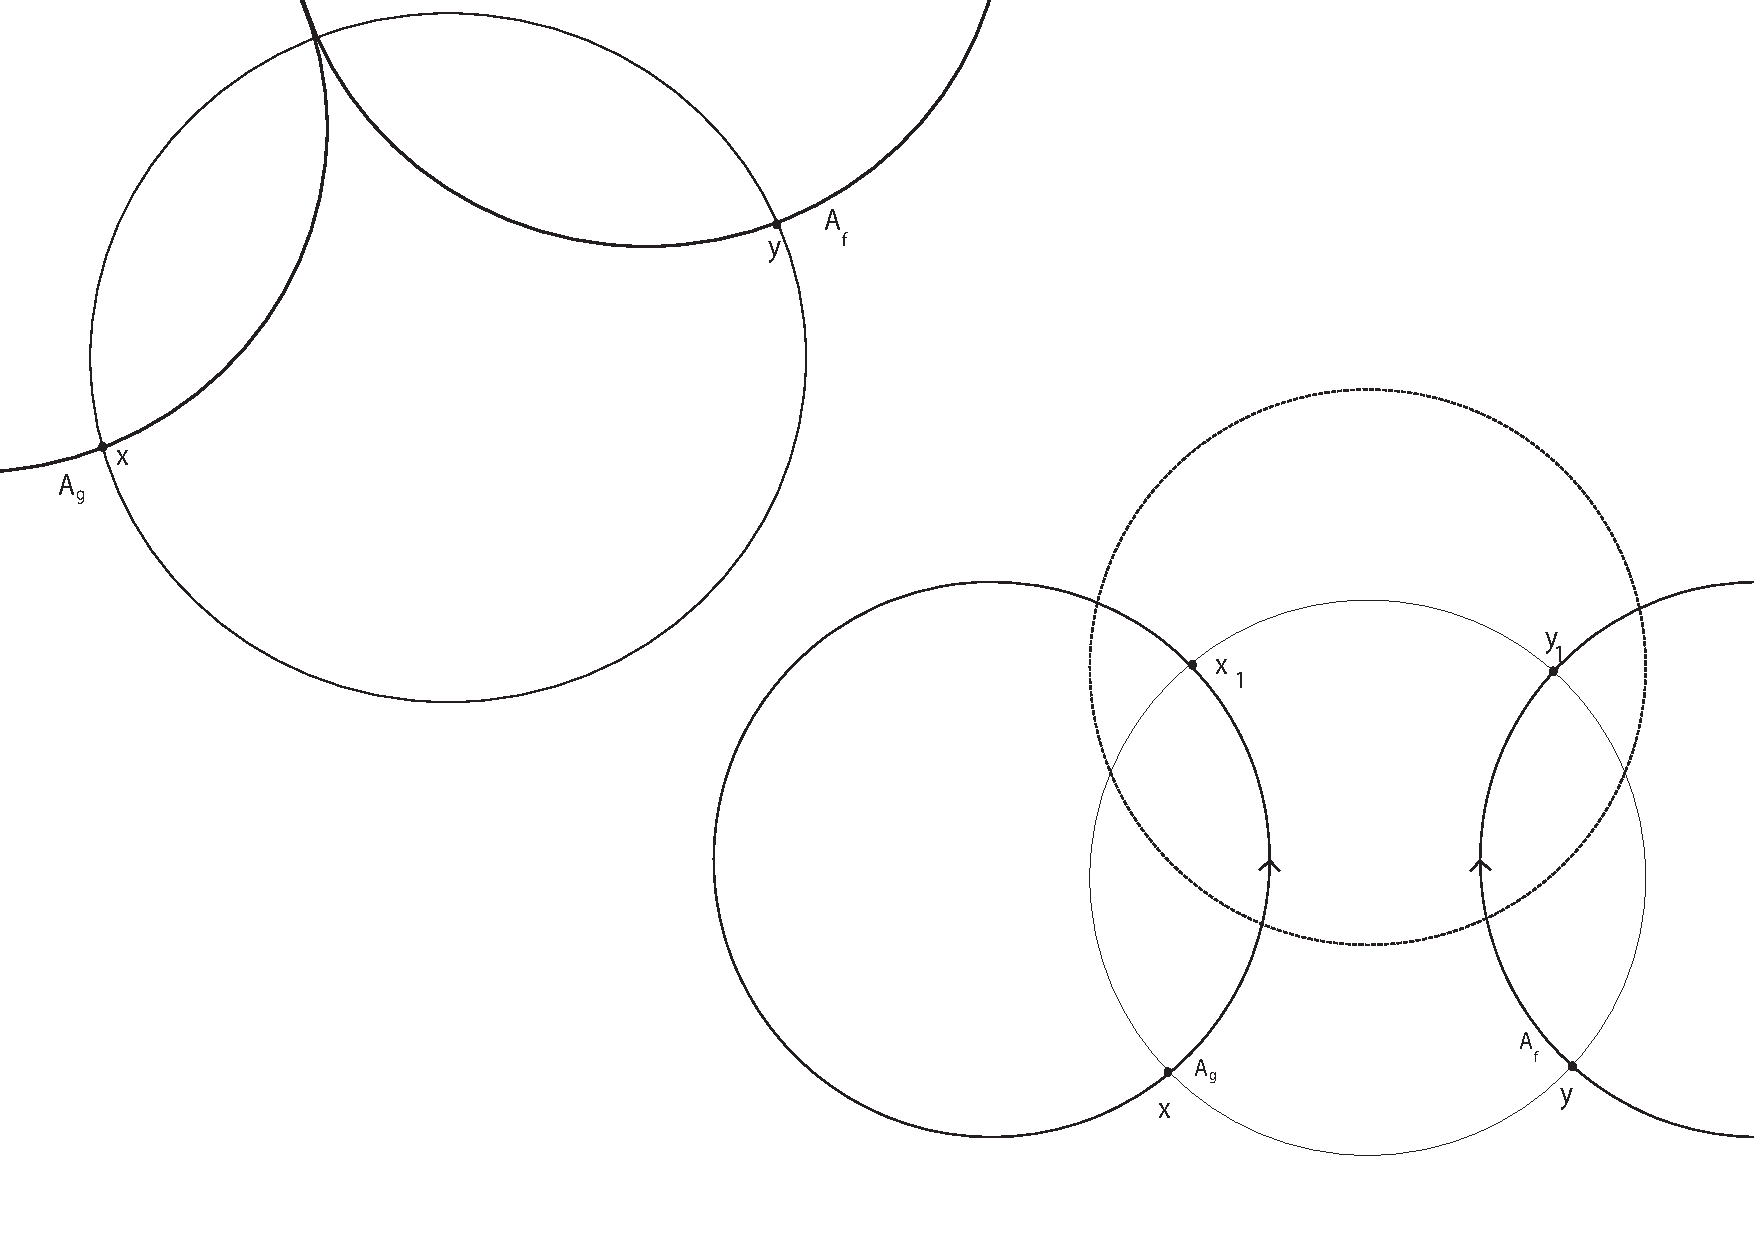
\includegraphics[width=10cm]{lemma6-dibujo-1-2}\\
  \caption{Ejes de f y g paralelos y divergentes}\label{lemma6-dibujo-1-2}
\end{figure}



M\'as a\'un debe haber elementos hiperb\'olicos en $G$, de otro modo
solo tendr\'ia elementos parab\'olicos que por hip\'otesis no
tendrian un punto fijo en com\'un y el lema \ref{lema3} implicar\'ia
una contradicci\'on en este caso. \\

Sea $f$ hiperb\'olico en $G$ y $A_{f} $ su eje y $\lambda_{f}$ la
medida de su desplazamiento, sea $g \in G$ tal que $fg \neq gf$,
entonces $f' = gf^{\pm 1}g^{-1}$ es una hiperb\'olico con el mismo
desplazamiento que $f$ y con eje $gA_{f} \neq A_{f}$ (Por no ser
permutables)(Si $A_{f}=gA_{f} \Rightarrow gfg^{-1}=f$ o
$gfg^{-1}=f^{-1}$. El primer caso es trivial. El segundo caso basta tomar un punto fijo $x$ de $f$ tal que  $g(x)$ no es punto fijo de $f$ (ni de $f^{-1}$) y evaluar en ambos lados de la ecuaci\'on para llegar a una contradicci\'on.) \\

$A_{f},A_{f'}$ no pueden ser paralelas por el lema \ref{lema5}, si
son divergente sea $\delta$ la distancia entre ellas y elijamos $f'$
tal que el exponente de $f$ haga $f$ y $f'$ con desplazamientos
opuestos, por las condiciones impuestas en $G$, $ff'$ no es
el\'iptico y del \ref{lema1} obtenemos

\begin{equation} \label{relacionseno1}
 \  senh \frac{1}{2}
\delta senh \frac{1}{2} \lambda_{f} \geqq 1
\end{equation}

Si $A_{f},A_{f'}$ son concurrentes sea $\phi$ su \'angulo de
intersecci\'on, dado que $[f,f']$ no es una rotaci\'on,  del
\ref{lema2} tenemos

\begin{equation} \label{relacionseno2}
 \ sen \phi senh^{2}\frac{1}{2} \lambda_{f} \geqq 1
\end{equation}

Estas desigualdades se aplican a $g$ fijo y $f$ variando.



\begin{figure}[h]
  \centering
  % Requires \usepackage{graphicx}
  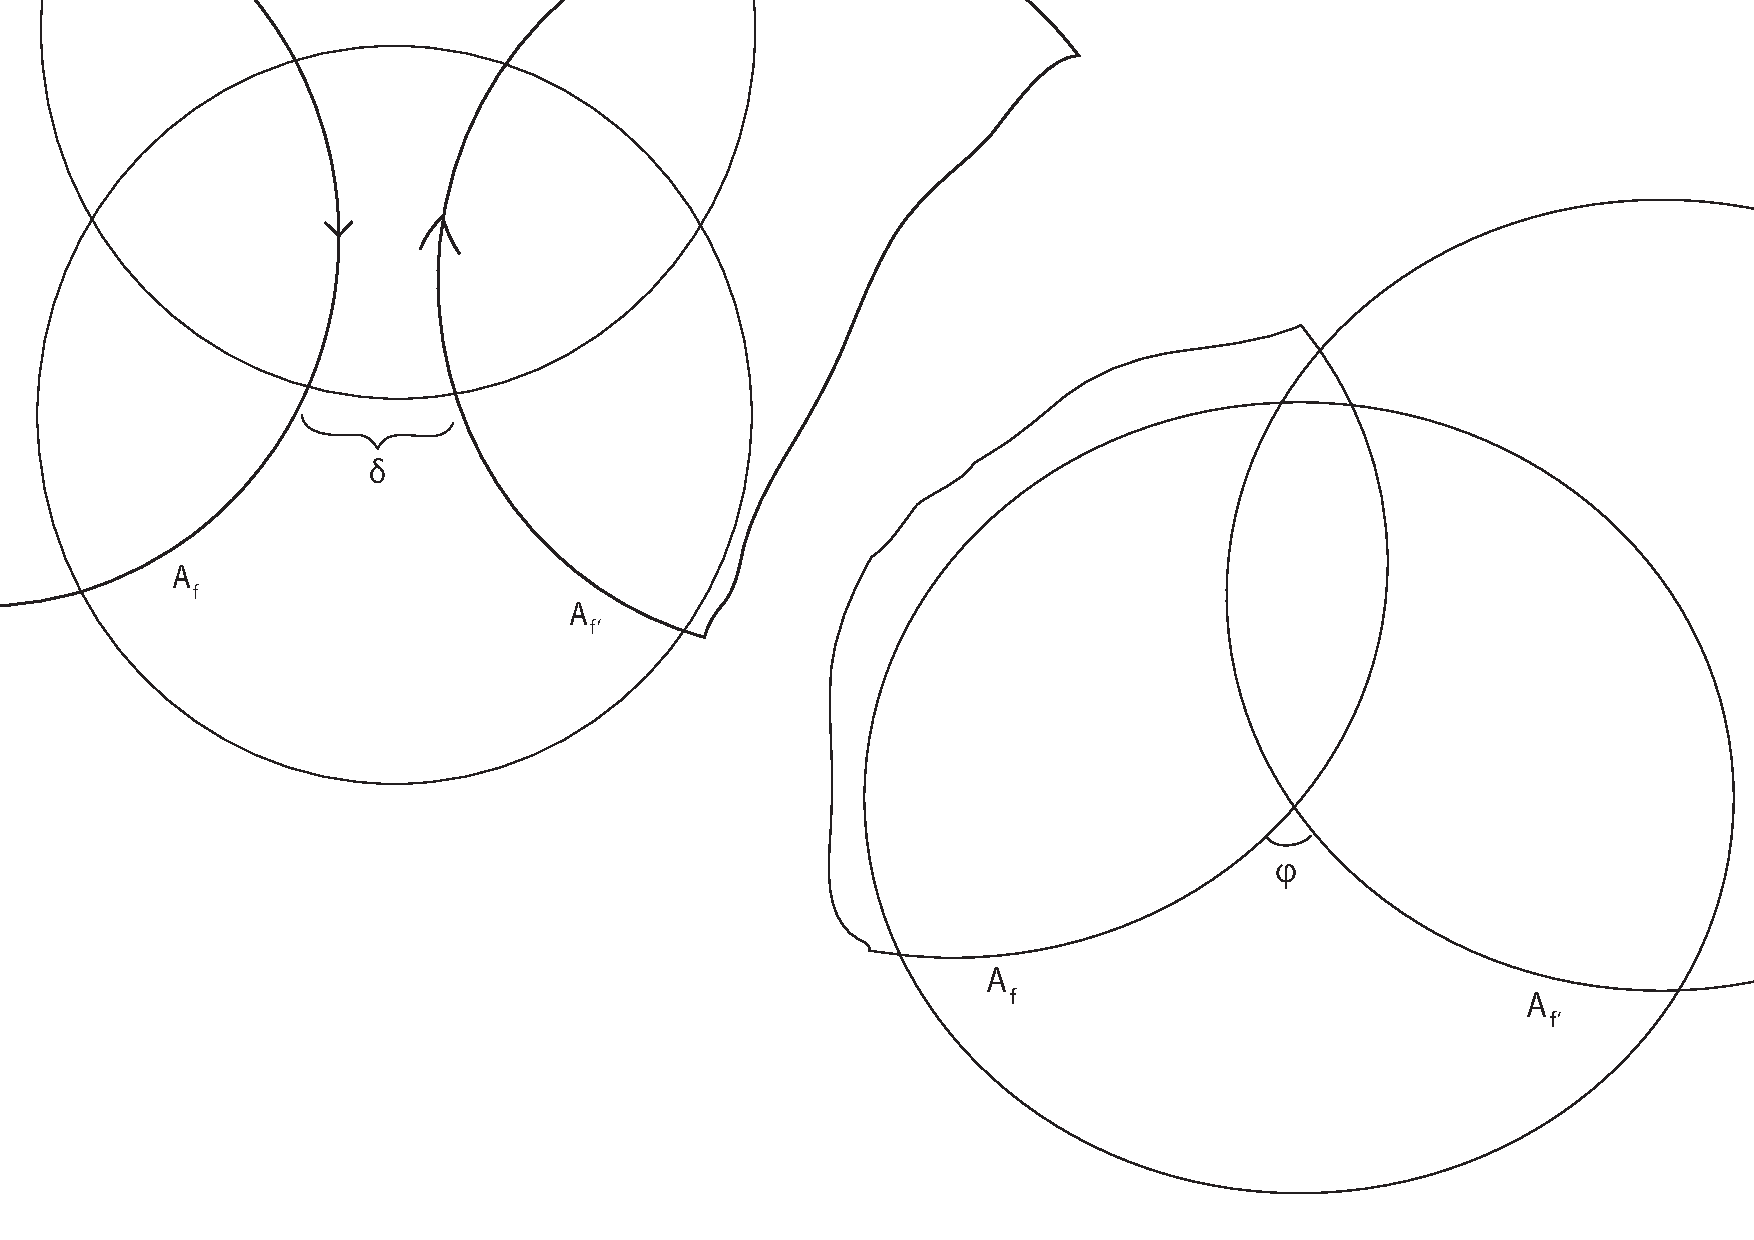
\includegraphics[width=9cm]{lemma6-dibujo-2-4}\\
  \caption{Figura \ref{lemma6-dibujo-2-4}}\label{lemma6-dibujo-2-4}
\end{figure}


Sea $A$ un eje de un elemento hiperb\'olico en $G$, los elementos
hiperb\'olicos que comparten este eje forman un subgrupo abeliano
$S_{A}$ de $G$, sea $g \in G$ un elemento que no tenga como eje a
$A$, es decir que no permuta con los elementos de $S_{A}$, se tiene
que $gA \neq A$. Si $gA$ y $A$ son divergentes digamos que su distancia es $d_{H}(gA,A)= \delta$
si $gA$ y $A$ son concurrentes digamos que se cortan en un \'angulo $\phi$. Dependiendo cual sea el caso aplicaremos \ref{relacionseno1} o \ref{relacionseno2}. \\


Si $f$ varia sobre todos los elementos de $S_{A}$, podemos notar que
todos tienen desplazamiento mayor que un n\'umero positivo distinto
de 1,por las condiciones \ref{relacionseno1} y \ref{relacionseno2} y sabiendo que $senhx \rightarrow 0$ cuando $x \rightarrow 0 $, $\lambda_{f}$ no puede ser arbitrariamente pequeño, m\'as a\'un los desplazamientos no pueden ser arbitrariamente cercanos a la cota, si asi fuera podemos encontrar dos elementos tal que su composici\'on tiene un desplazamiento menor que la cota dada. Entonces $S_{A}$ es discontinuo. Sea $\lambda_{0}$ el desplazamiento mas pequeño de elementos de $S_{A}$ que por lo anterior existe.  \\

Podemos aplicar las mismas desigualdades para $f \in S_{A}$ fijo y
$g $ variando sobre los representantes $g_{1},g_{2},...$ de las
clases de $S_{A} < G$ ($g_{1} \backsim g_{2} \Leftrightarrow
g_{1}S_{A} = g_{2}S_{A} \Leftrightarrow g_{1}g_{2}^{-1} \in S_{A}$).

\begin{rem}
Si $g_{1} \backsim g_{2} \Rightarrow g_{1}A=g_{2}A$ ya que
$g_{1}g_{2}^{-1} = f \in S_{A} \Rightarrow g_{1}g_{2}^{-1}A = fA
\Rightarrow g_{1}g_{2}^{-1}A = A \Rightarrow g_{2}^{-1}A =
g_{1}^{-1}A$
\end{rem}

Los ejes de los elementos hiperb\'olicos $f_{v}=
g_{v}fg_{v}^{-1}$ varian sobre los diferentes ejes de la clase de
equivalencia $GA$ de $A$. \\

Dado que $f_{v}$ tiene el mismo desplazamiento $\lambda_{f}$ que $f$
para todo \'indice $v$, de \ref{relacionseno1} y \ref{relacionseno2} obtenemos que
$senh\frac{1}{2} \delta $ y $sen \phi$ tienen una cota inferior por
lo que $\delta$ y $\phi$ tambi\'en la tienen seg\'un sean
divergentes o concurrentes los ejes $g_{v}A$, esto implica que los
ejes no se acumulan en $D$.  \\


Sea $x \in A$. Todo punto en $Gx$ esta en alg\'un elemento del
conjunto $g_{v}A$. Para un eje dado los puntos $Gx$ que se
encuentran en este eje forman una sucesi\'on de puntos equidistantes
a distancia $\lambda$ (Los puntos en $Gx \cap g_{v}A$ son los puntos
$gx,hx$ tal que $g \backsim h $, luego para $gx,hx \in g_{v}A
\Rightarrow d_{H}(gx,hx)=d_{H}(x,g^{-1}hx), g^{-1}h \in S_{A}
\Rightarrow \lambda_{g^{-1}h} \geqq \lambda_{0}$ (Fig. \ref{lemma6-dibujo6}). \\

\begin{figure}[h]
  \centering
  % Requires \usepackage{graphicx}
  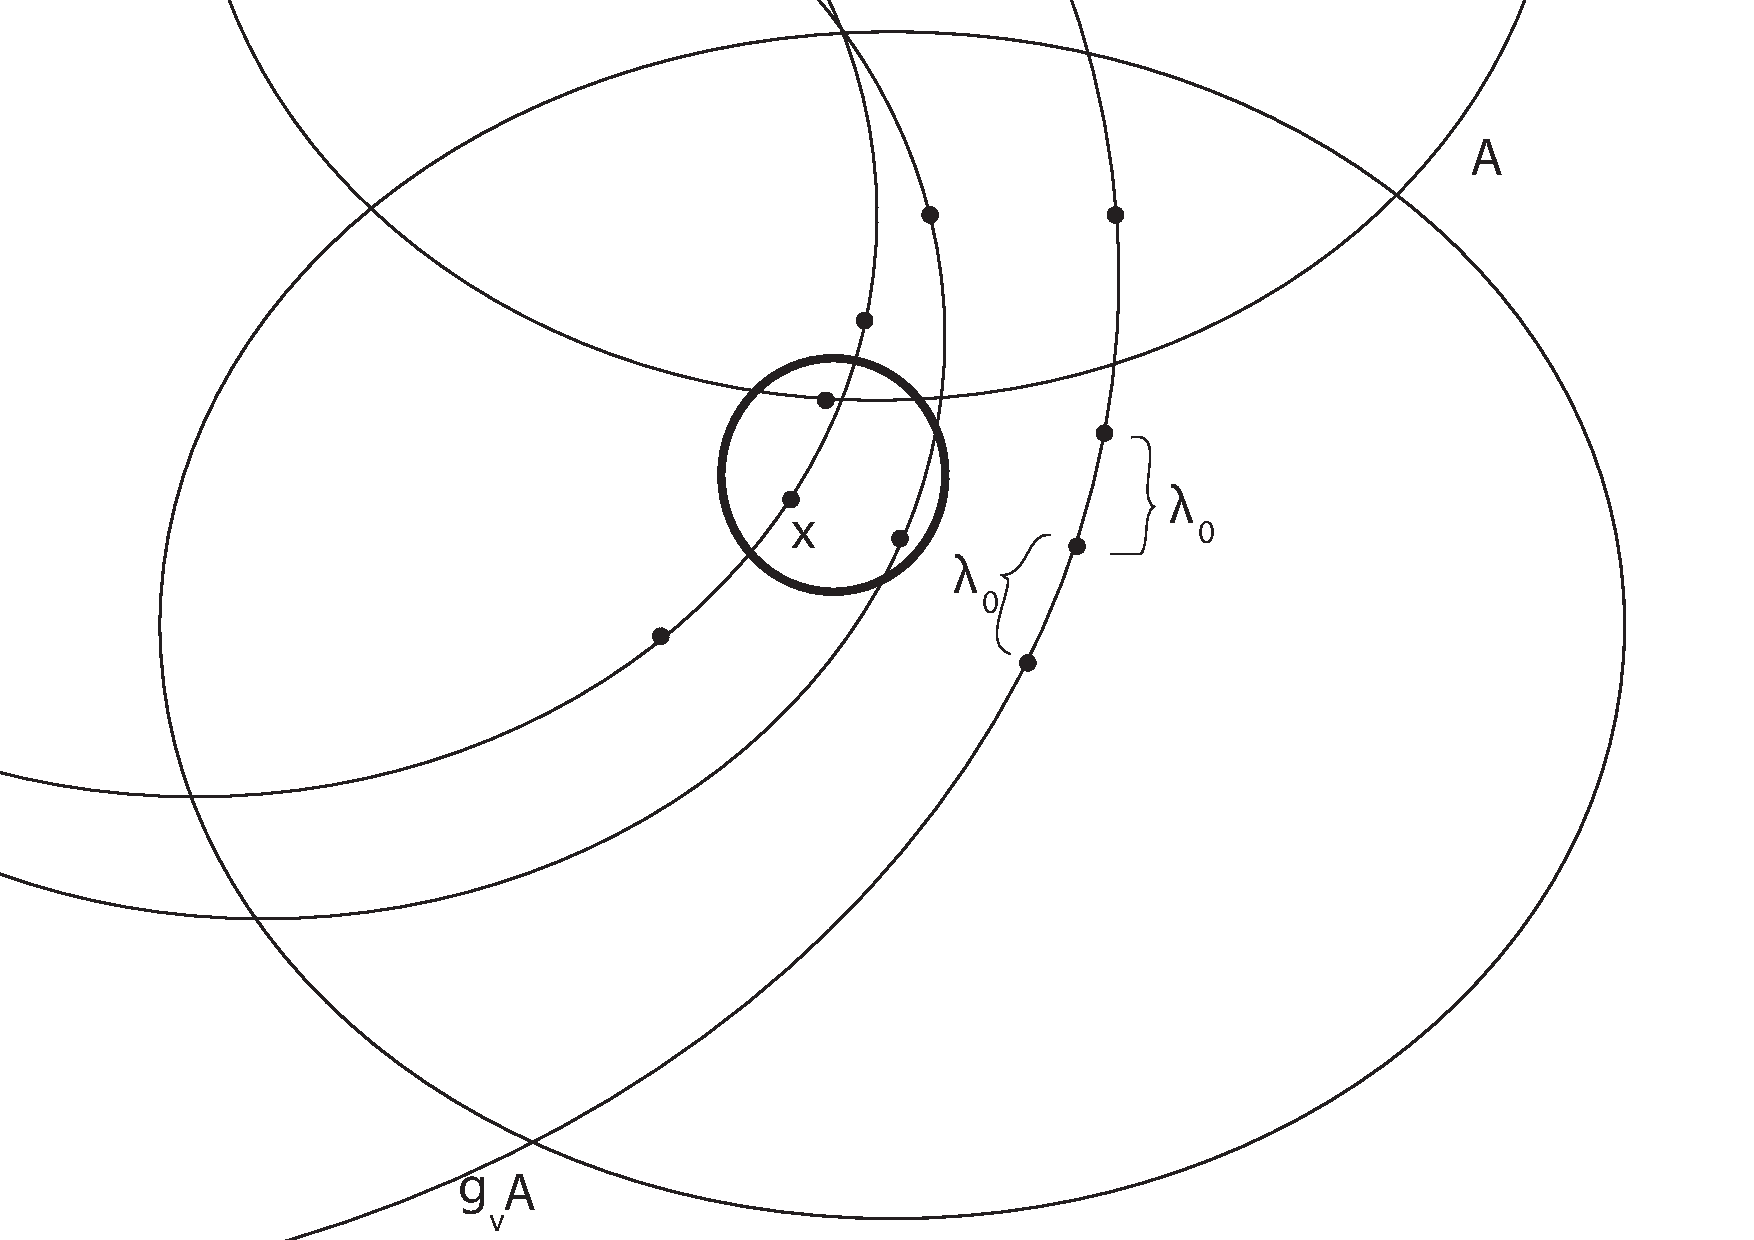
\includegraphics[width=10cm]{lemma6-dibujo6}\\
  \caption{Figura \ref{lemma6-dibujo6}}\label{lemma6-dibujo6}
\end{figure}


El c\'irculo con centro $x$ y radio $\frac{1}{2} \lambda_{0}$
no puede contener mas de un punto de dicha sucesi\'on en su
interior, entonces el n\'umero de puntos en $Gx$ dentro de este
c\'irculo es a lo m'as igual al n\'umero de ejes $g_{v}A$ que cortan
al c\'irculo, este n\'umero es finito ya que los ejes $g_{v}A$ no se
acumulan en $D \  \therefore \ x$ no es punto de acumulaci\'on de
$Gx$. $_{\square}$



\section{Un ejemplo de un grupo discreto}

En el cap\'itulo \ref{cha:grupo schottky} hallamos un grupo de Schottky que es un subgrupo discreto de isometrias hiperb\'olicas, m\'as a\'un sabemos que todos los elementos no triviales del grupo de Schottky son loxodr\'omicos, en nuestro caso hiperb\'olicos, excepto por la identidad, para que podamos validar el teorema de Nielsen en este grupo debemos verificar que se cumplen las condiciones del teorema. Los generadores del grupo de Schottky son hiperb\'olicos por lo cual cada uno tiene una geodesica invariante, podemos usar las matrices del grupo de monodrom\'ia de la ecuaci\'on diferencial hipergeometrica \ref{Matrices_teorema_monodromia_grupo} que son conjugadas a los generadores del grupo de Schottky;

$$  A_{0} =  \begin{pmatrix}
 1& 0\\
 0& \varepsilon (-c)
 \end{pmatrix}  ,\ \ \
A_{1} = P ^{-1}\begin{pmatrix}
 1& 0\\
 0& \varepsilon (c-a-b)
 \end{pmatrix} P
$$


Notamos que $A_{0}$ fija $0,\infty$ y por tanto deja invariante la geod\'esica que los une, podemos ver que $A_{1}$ fija $P^{-1}(0)$ y $P^{-1}(\infty)$ y dado que conocemos $P^{-1}$ podemos calcular ambos valores, por un lado $P^{-1}(0)= \frac{-C}{D}$ por otro lado $P^{-1}(\infty) = \frac{-A}{B}$, y por tanto deja invariante la geod\'esica que une estos dos puntos. Mas abajo probamos que estos dos ejes necesariamente son divergentes.

 En nuestro caso tenemos un grupo de Schottky con dos generadores, sabemos que es libre y tambi\'en es no elemental (\ref{def:elemental}). En \cite{Beardon} encontramos un teorema que dice que para un grupo de transformaciones hiperb\'olicas con las caracteristicas anteriores ser discreto equivale a que act\'ue de manera discontinua seg\'un \ref{def:discontinuo1}, de igual manera en \cite{Beardon} encontramos que \ref{def:discontinuo1} implica \ref{def:discontinuo2}.

 Por otro lado $\Lambda_{\theta}$ posee, salvo la identidad, solo elementos hiperb\'olicos, para aplicar el teorema de Nielsen necesitamos adem\'as que el grupo no tenga ni puntos fijos ni rectas invariantes como mencionamos arriba. En \cite{Beardon} encontramos el siguiente teorema;

\begin{thm}
 Dos transformaciones de Mobius $g,h$ tienen un punto fijo en $\widehat{\mathbb{C}}$ si y solo si $tr[g,h]=2$
\end{thm}

 Haciendo los calculos correspondientes a las matrices asociadas a $\gamma_{1},\gamma_{2}$ obtenemos que; $tr[\gamma_{1},\gamma_{2}] = \frac{2T^{2}(R^{2}-C^{2}) + C^{2}(T^{4} +1)}{T^{2}R^{2}}$, si suponemos que $tr[\gamma_{1},\gamma_{2}]=2$ obtenemos que $C^{2}=0$ o que $T= \pm 1$, ninguno de estos casos es posible debido a las condiciones exigidas, por lo que $tr[\gamma_{1},\gamma_{2}] \neq 2$ es decir $\gamma_{1},\gamma_{2}$  no tienen puntos fijos en $\widehat{\mathbb{C}}$ (en particular no los tiene en $D$) y dado que tienen ejes diferentes, estos necesariamente son divergentes de otro modo su intersecci\'on ser\'ia un punto fijo, por tal motivo no hay rectas invariantes en el grupo generado por estos elementos.Aplicando el teorema de Nielsen se puede concluir que $\Lambda_{\theta}$ es discontinuo en $D$.

Todo lo anterior nos permite afirmar que la familia de  grupos de Schottky hallada en \ref{cha:grupo schottky} son ejemplos en donde podemos verificar el teorema de Nielsen. En la actualidad existen muchos resultados que nos dan la misma informaci\'on que este teorema pero la exposici\'on geom\'etrica de este resultado sigue siendo admirable gracias a su demostraci\'on basada en su mayoria en la geometr\'ia hiperb\'olica pura.


%----------------------------------------------------------------------

	
	

% --------------------------------------------------------------
%:                  BACK MATTER: appendices, refs,..
% --------------------------------------------------------------

% the back matter: appendix and references close the thesis
\backmatter


%: ----------------------- appendix ------------------------

\appendix


% this file is called up by thesis.tex
% content in this file will be fed into the main document

%: ----------------------- introduction file header -----------------------


\chapter{Ap\'endice}
\label{cha:apendice}

\section{Igualdades trigonom\'etricas}

Dedicamos esta secci\'on a recopilar las f\'ormulas de trigonometr\'ia hiperb\'olica utilizadas durante \'este trabajo. Comenzamos con las f\'ormulas para seno y coseno hperb\'olicos:

 \begin{eqnarray}
 cosh(x \pm y)= coshxcoshy \pm sinhxsinhy \\
 sinh(x \pm y)=sinhxcoshy \pm coshxsinhy \\
 cosh2x=cosh^{2}x+sinh^{2}x=2cosh^{2}x-1 \\
 sinh2x = 2sinhx\cdot coshx
 \end{eqnarray}

 Para tri\'angulos hiperb\'olicos tenemos lo siguiente: \\

 Sea $\vartriangle (A,B,C)$ un tri\'angulo con lados $A, B $ y $ C$. Y sean sus correspondientes \'angulos opuestos $\alpha,\beta$ y $\gamma$ entonces, si $\gamma$ es un angulo recto tenemos; \\

 Ley de los cosenos hiperb\'olicos
 \begin{equation}
 cosh C = cosh A\cdot cosh B
 \end{equation}

 Ley de los senos hiperb\'olicos
 \begin{equation}
 sinhB = sinhA \cdot tan \beta
 \end{equation}

 Tambi\'en
 \begin{eqnarray}
 cosh A \cdot sin \beta = cos \alpha  \\
 coshB \cdot sin \alpha= cos \beta
 \end{eqnarray}

 Para tri\'angulos arbitrarios se tiene; \\

 Ley de los cosenos hiperb\'olicos
 \begin{equation}
 coshC=coshA \cdot coshB - sinhA\cdot sinhB\cdot cos \gamma
 \end{equation}

Ley de los senos hiperb\'olicos
\begin{equation}
\frac{sinhA}{sin \alpha} =\frac{sinhB}{sin \beta}= \frac{sinhC}{sin \gamma}
\end{equation}

Para un cuadrilatero con tres \'angulos rectos como en la figura \ref{apendice1}, donde $\Phi$ no es recto, se tiene:

\begin{eqnarray}
sinhD\cdot sinhA =cos \Phi \\
cosh D = cosh B \cdot sin \Phi \\
coshA=coshC\cdot sin \Phi
\end{eqnarray}

\begin{figure}[h]
  \centering
  % Requires \usepackage{graphicx}
  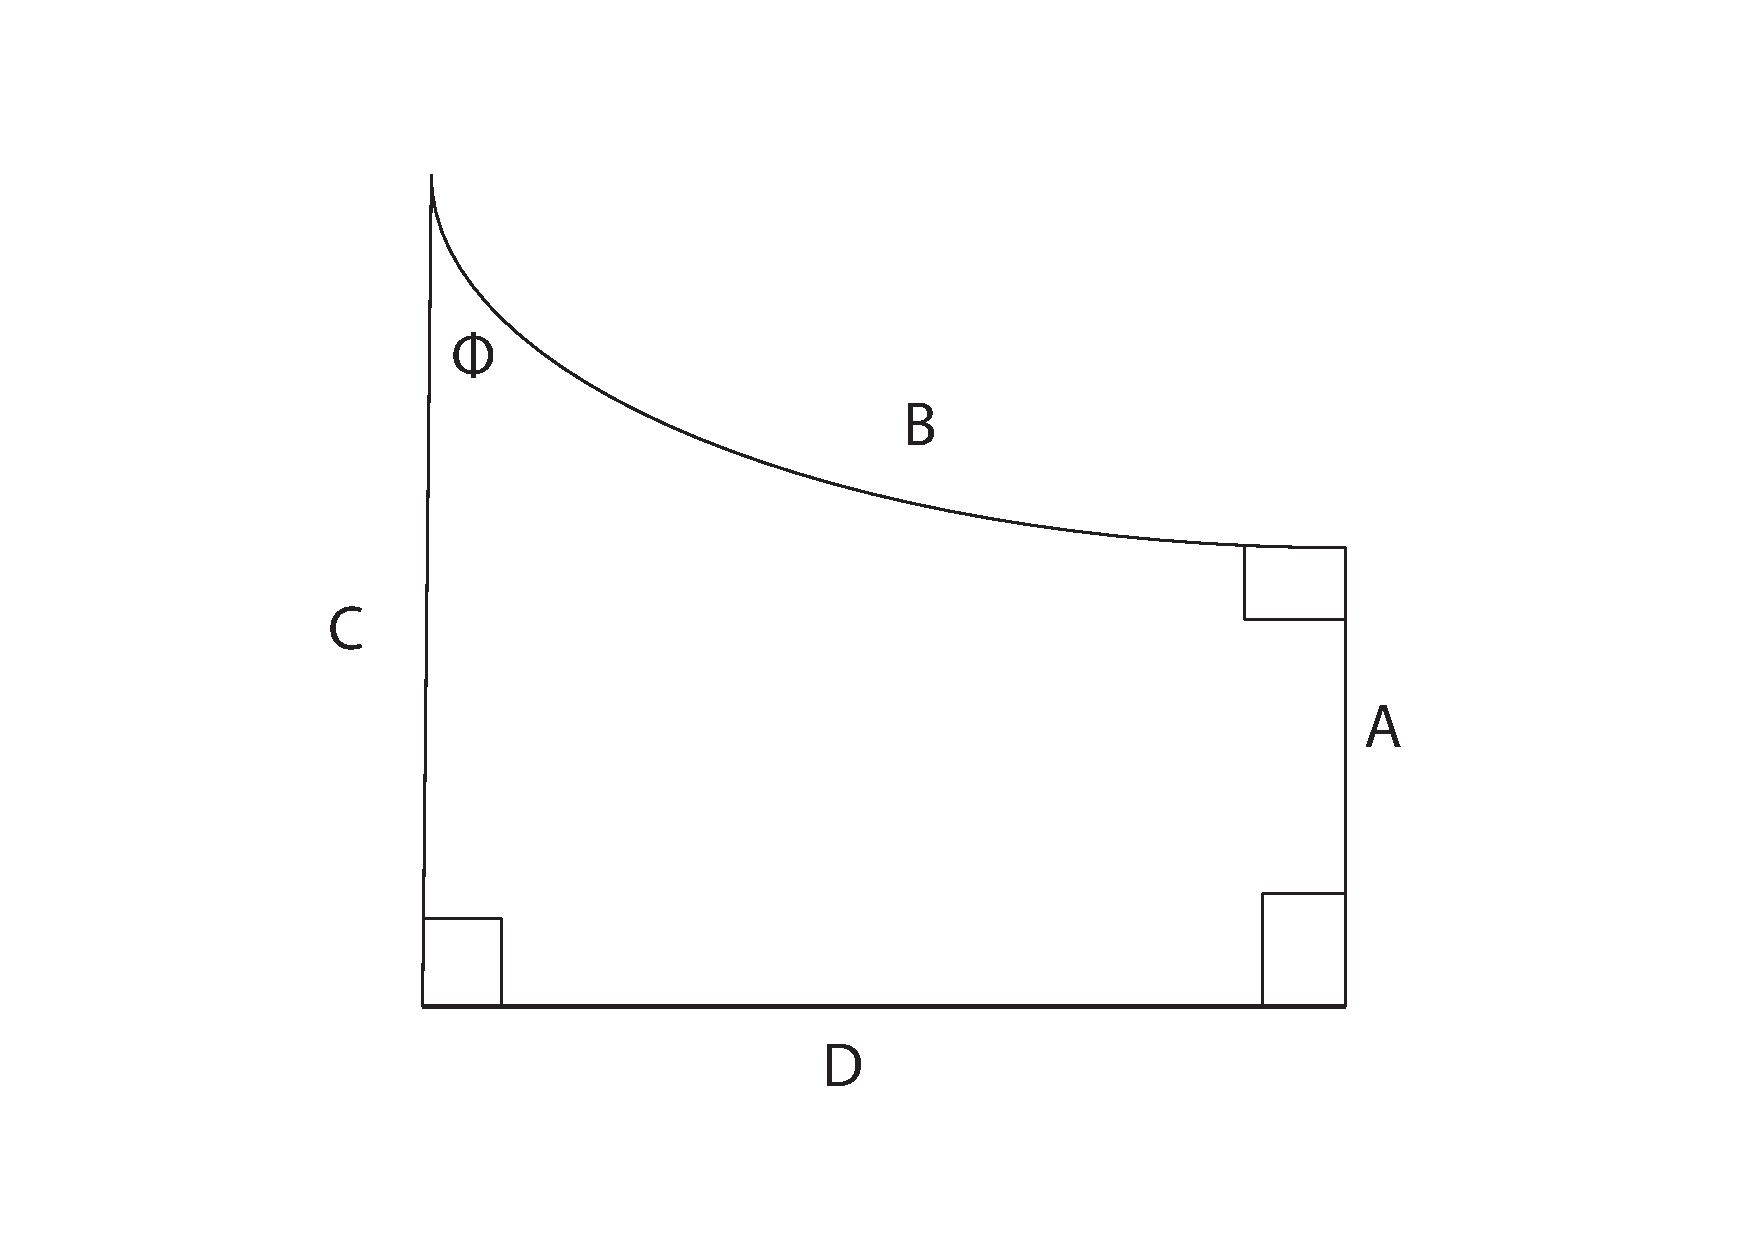
\includegraphics[width=10cm]{apendice1}\\
  \caption{Cuadrilatero con 3 \'angulos rectos}\label{apendice1}
\end{figure}

En un tri\'angulo $\vartriangle (A,B,C)$ hay una relaci\'on entre $\gamma$ y la longitud de $C$

$$coshC > coshA\cdot coshB \ si \ \gamma < \frac{\pi}{2}$$
$$ coshC = coshA \cdot coshB \ si  \ \gamma= \frac{\pi}{2}$$
$$ coshC < coshA \cdot coshB \ si \ \gamma > \frac{\pi}{2}$$

Por \'ultimo tenemos un resultado para pentagonos con 4 \'angulos rectos.

Sea $P$ un pent\'agono como en la figura \ref{apendice2}, donde $h,D$ son medidas de los lados  y $H$ la medida de la perpendicular del v\'ertice al lado $s$ y denotamos por $s$ tambi\'en a su medida.

\begin{figure}[h]
  \centering
  % Requires \usepackage{graphicx}
  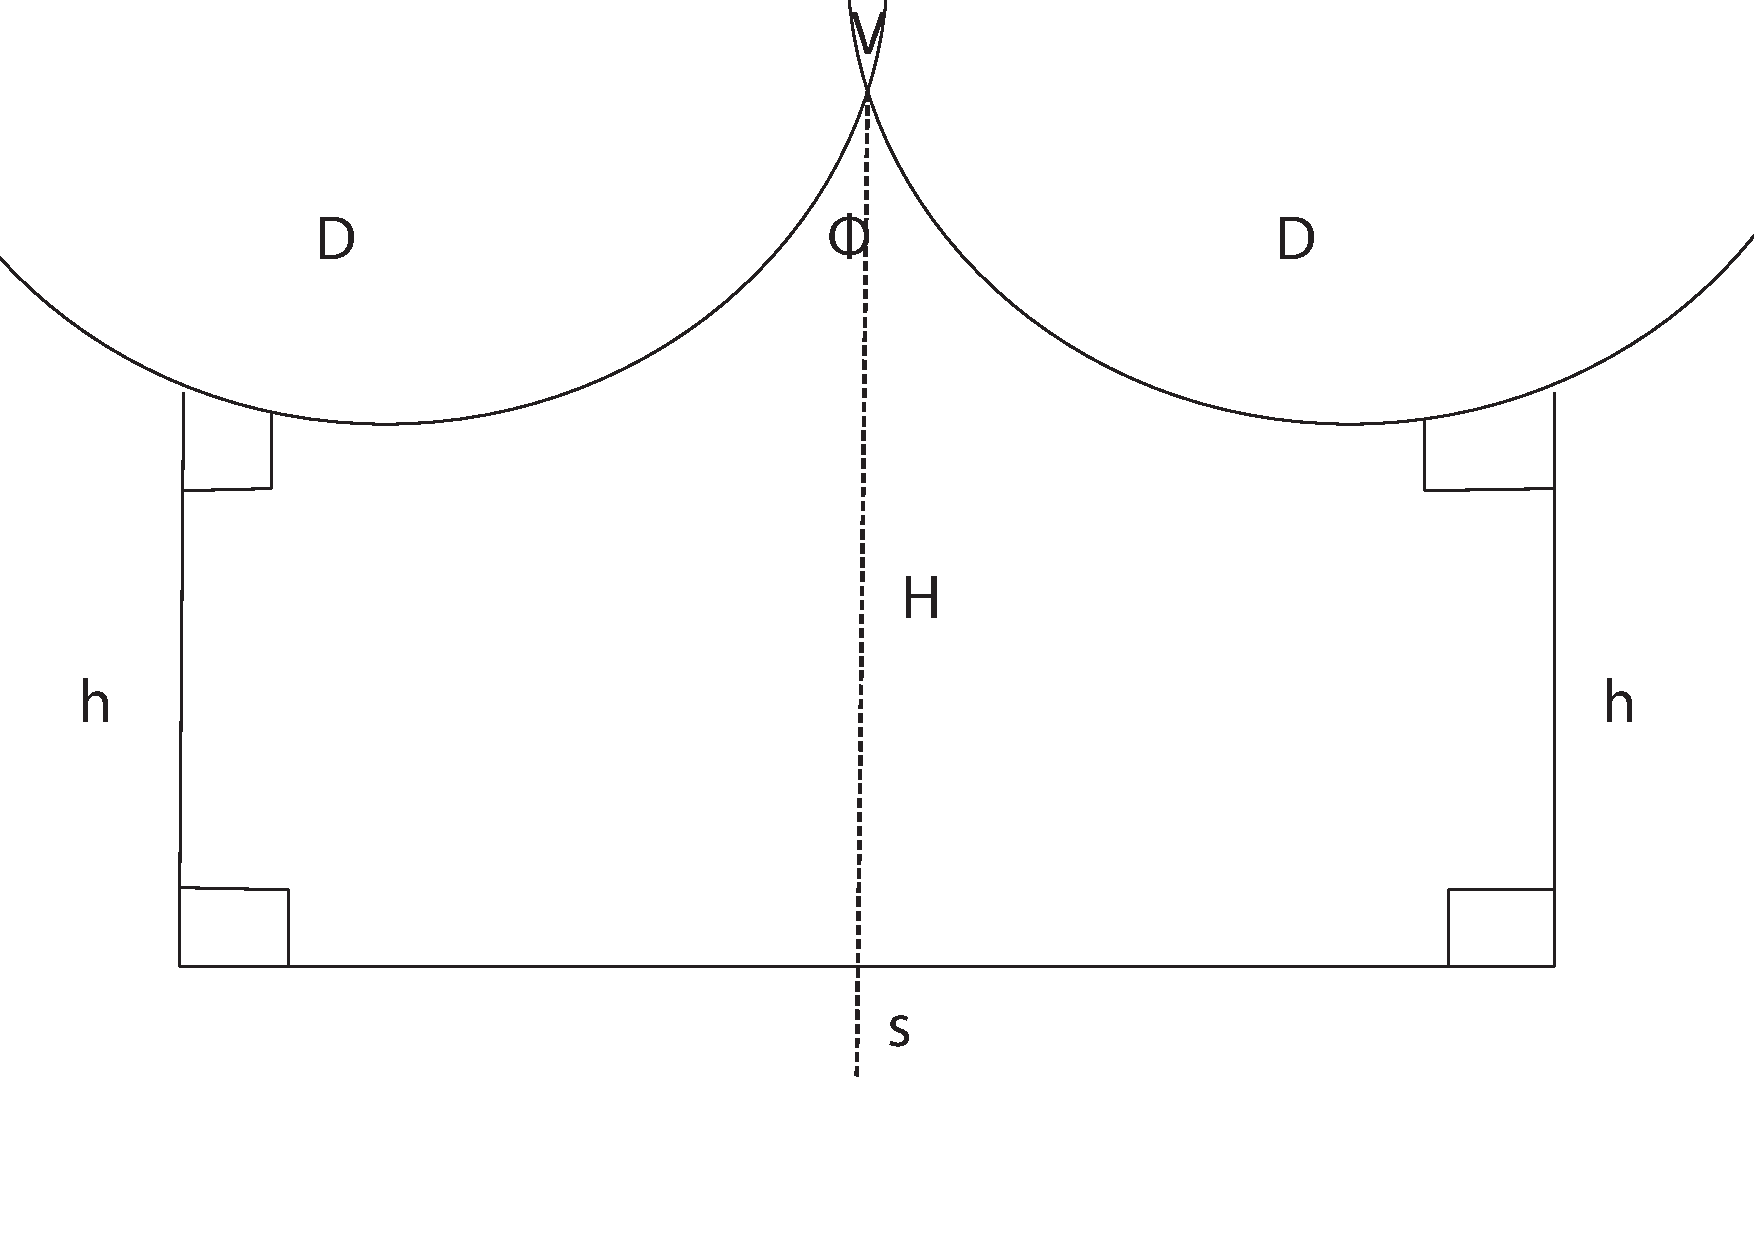
\includegraphics[width=10cm]{apendice2}\\
  \caption{Pent\'agono con 4 \'angulos rectos}\label{apendice2}
\end{figure}

Las siguientes condiciones se cumplen 

\begin{eqnarray}
sinh \cdot sinh \frac{s}{2}= cos (\frac{\Phi}{2}) \\
cosh=coshH \cdot sin (\frac{\Phi}{2}) \\
cosh \frac{s}{2} = coshD \cdot sin (\frac{\Phi}{2})
\end{eqnarray}


\section{Teorema de Cauchy}


\section{Mapeo y principio de reflexi\'on de Schwarz}

Si consideramos la ecuaci\'on diferencial hipergeom\'etrica 

$$ x(1-x)u''+(c-(a+b+1)x)u'-abu=0$$

Cualesquiera dos soluciones linealmente independientes $u_{1},u_{2}$ definen un mapeo

$$s: \mathbb{C}-\lbrace 0,1 \rbrace \ni x \mapsto u_{1}(x):u_{2}(x) \in \widehat{\mathbb{C}} $$

Al que llamamos el mapeo de Schwarz. El teorema fundamental de Cauchy nos asegura que dos soluciones linealmente independientes no son simultaneamente cero en $\mathbb{C}-\lbrace 0,1 \rbrace $. Para un estudio mas profundo del mapeo de Scwarz se remite al lector a \cite{geometricstudy}.

EL principio de reflexi\'on de Schwarz se enuncia de la siguiente manera:

\begin{prop}
Sea $f$ una funci\'on holomorfa en un dominio $D$ cuya frontera contiene un intervalo real $(a,b)$. Supongamos que $f$ se puede extender a una funci\'on continua en $D \cup (a,b)$ y es real valuada en el intervalo $(a,b)$. Extendiendo $f$ por

$$f(x):= \bar{f(\bar{x})}, \ x\in \bar{D}:= \lbrace \bar{\xi} | \xi \in D \rbrace $$

A la imagen reflejada $\bar{D}$ de $D$. Entonces, la extensi\'on de $f$ es holomorfa en $D \cup (a,b) \cup \bar{D}$, y su imagen es la uni\'on de $f(D)$, su imagen reflejada $\bar{f(D)}$ y el intervalo $f((a,b))$ que comparten como parte de su frontera. 
\end{prop}

\begin{figure}[h]
  \centering
  % Requires \usepackage{graphicx}
  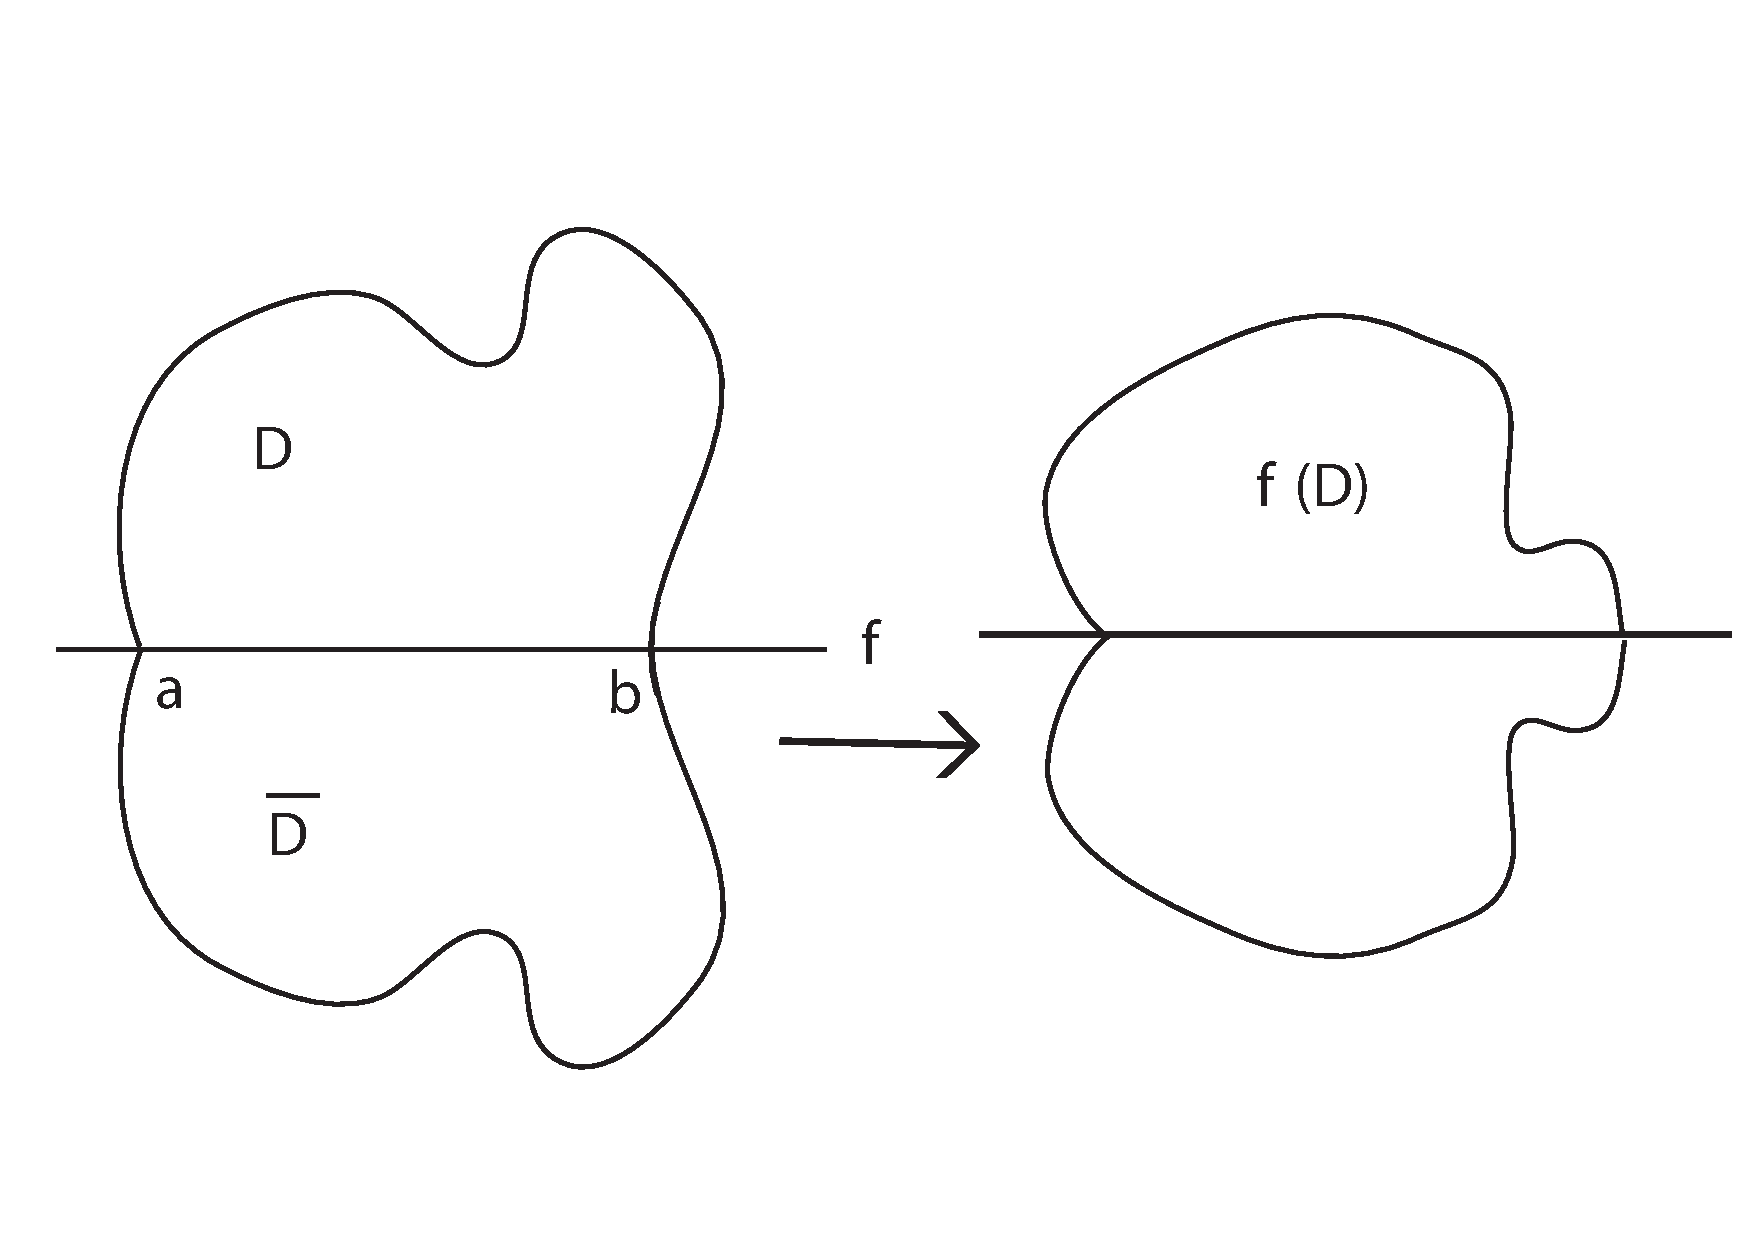
\includegraphics[width=10cm]{apendice3}\\
  \caption{Principio de reflexi\'on de Schwarz}\label{apendice3}
\end{figure}



% the code below specifies where the figures are stored
\ifpdf
    \graphicspath{{5_conclusion/figures/PNG/}{5_conclusion/figures/PDF/}{5_conclusion/figures/}}
\else
    \graphicspath{{5_conclusion/figures/EPS/}{5_conclusion/figures/}}
\fi


%-------------------------------------------------------------------------


% ----------------------------------------------------------------------








%: ----------------------- bibliography ------------------------



% The section below defines how references are listed and formatted
% The default below is 2 columns, small font, complete author names.
% Entries are also linked back to the page number in the text and to external URL if provided in the BibTex file.


% Original version:

% PhDbiblio-url2 = names small caps, title bold & hyperlinked, link to page
%\begin{multicols}{2} % \begin{multicols}{ # columns}[ header text][ space]
%\begin{tiny} % tiny(5) < scriptsize(7) < footnotesize(8) < small (9)
%
%\bibliographystyle{Latex/Classes/PhDbiblio-url2} % Title is link if provided
%\renewcommand{\bibname}{References} % changes the header; default: Bibliography
%
%\bibliography{9_backmatter/references} % adjust this to fit your BibTex file
%
%\end{tiny}
%\end{multicols}



% Show all bibliography entries
%\nocite*



% If we want bibliography backreference, use unsrt first and the desidered one after

%\bibliographystyle{unsrt} % Defines the bibliography style

\bibliographystyle{alpha} % Defines the bibliography style

%\bibliographystyle{apa-good} % Defines the bibliography style
%\bibliographystyle{natbib} % Defines the bibliography style

%\bibliographystyle{plainurl}

%\renewcommand{\bibname}{References} % changes the header; default: Bibliography

%To include the references/works cited/bibliography in your Table of Contents, right before the bibliography command, use the command
%\addcontentsline{toc}{section}{References}
%

\bibliography{9_backmatter/references} % adjust this to fit your BibTex file

% --------------------------------------------------------------
% Various bibliography styles exit. Replace above style as desired.

% in-text refs: (1) (1; 2)
% ref list: alphabetical; author(s) in small caps; initials last name; page(s)
%\bibliographystyle{Latex/Classes/PhDbiblio-case} % title forced lower case
%\bibliographystyle{Latex/Classes/PhDbiblio-bold} % title as in bibtex but bold
%\bibliographystyle{Latex/Classes/PhDbiblio-url} % bold + www link if provided

%\bibliographystyle{Latex/Classes/jmb} % calls style file jmb.bst
% in-text refs: author (year) without brackets
% ref list: alphabetical; author(s) in normal font; last name, initials; page(s)

%\bibliographystyle{plainnat} % calls style file plainnat.bst
% in-text refs: author (year) without brackets
% (this works with package natbib)


% --------------------------------------------------------------


%: Declaration of originality

% this file is called up by thesis.tex
% content in this file will be fed into the main document

%: ----------------------- introduction file header -----------------------


% the code below specifies where the figures are stored
\ifpdf
    \graphicspath{{9_backmatter/figures/PNG/}{9_backmatter/figures/PDF/}{9_backmatter/figures/}}
\else
    \graphicspath{{9_backmatter/figures/EPS/}{9_backmatter/figures/}}
\fi

% Thesis statement of originality -------------------------------------

% Depending on the regulations of your faculty you may need a declaration like the one below. This specific one is from the medical faculty of the university of Dresden.





%-------------------------------------------------------------------------

\thispagestyle{empty}

\hfill
\vfill
\medskip


\vfill
\medskip
\vspace{1cm}
\bigskip


%-------------------------------------------------------------------------

% Blank page
\clearpage
\thispagestyle{empty}

\hfill
\vfill
\medskip

\begin{center}
\textit{This page is intentionally left blank}
\end{center}

\vfill
\medskip
\vspace{1cm}
\bigskip


% ----------------------------------------------------------------------





\end{document}
